\documentclass[twoside]{book}

% Packages required by doxygen
\usepackage{fixltx2e}
\usepackage{calc}
\usepackage{doxygen}
\usepackage[export]{adjustbox} % also loads graphicx
\usepackage{graphicx}
\usepackage[utf8]{inputenc}
\usepackage{makeidx}
\usepackage{multicol}
\usepackage{multirow}
\PassOptionsToPackage{warn}{textcomp}
\usepackage{textcomp}
\usepackage[nointegrals]{wasysym}
\usepackage[table]{xcolor}

% Font selection
\usepackage[T1]{fontenc}
\usepackage[scaled=.90]{helvet}
\usepackage{courier}
\usepackage{amssymb}
\usepackage{sectsty}
\renewcommand{\familydefault}{\sfdefault}
\allsectionsfont{%
  \fontseries{bc}\selectfont%
  \color{darkgray}%
}
\renewcommand{\DoxyLabelFont}{%
  \fontseries{bc}\selectfont%
  \color{darkgray}%
}
\newcommand{\+}{\discretionary{\mbox{\scriptsize$\hookleftarrow$}}{}{}}

% Page & text layout
\usepackage{geometry}
\geometry{%
  a4paper,%
  top=2.5cm,%
  bottom=2.5cm,%
  left=2.5cm,%
  right=2.5cm%
}
\tolerance=750
\hfuzz=15pt
\hbadness=750
\setlength{\emergencystretch}{15pt}
\setlength{\parindent}{0cm}
\setlength{\parskip}{0.2cm}
\makeatletter
\renewcommand{\paragraph}{%
  \@startsection{paragraph}{4}{0ex}{-1.0ex}{1.0ex}{%
    \normalfont\normalsize\bfseries\SS@parafont%
  }%
}
\renewcommand{\subparagraph}{%
  \@startsection{subparagraph}{5}{0ex}{-1.0ex}{1.0ex}{%
    \normalfont\normalsize\bfseries\SS@subparafont%
  }%
}
\makeatother

% Headers & footers
\usepackage{fancyhdr}
\pagestyle{fancyplain}
\fancyhead[LE]{\fancyplain{}{\bfseries\thepage}}
\fancyhead[CE]{\fancyplain{}{}}
\fancyhead[RE]{\fancyplain{}{\bfseries\leftmark}}
\fancyhead[LO]{\fancyplain{}{\bfseries\rightmark}}
\fancyhead[CO]{\fancyplain{}{}}
\fancyhead[RO]{\fancyplain{}{\bfseries\thepage}}
\fancyfoot[LE]{\fancyplain{}{}}
\fancyfoot[CE]{\fancyplain{}{}}
\fancyfoot[RE]{\fancyplain{}{\bfseries\scriptsize Generated on Tue Mar 8 2016 22\+:53\+:50 for P\+S-\/\+M\+M\+M \+: Parallel Simulator for (\+I\+M-\/)\+Miscible Multi-\/\+Phase Mixing Flow by Doxygen }}
\fancyfoot[LO]{\fancyplain{}{\bfseries\scriptsize Generated on Tue Mar 8 2016 22\+:53\+:50 for P\+S-\/\+M\+M\+M \+: Parallel Simulator for (\+I\+M-\/)\+Miscible Multi-\/\+Phase Mixing Flow by Doxygen }}
\fancyfoot[CO]{\fancyplain{}{}}
\fancyfoot[RO]{\fancyplain{}{}}
\renewcommand{\footrulewidth}{0.4pt}
\renewcommand{\chaptermark}[1]{%
  \markboth{#1}{}%
}
\renewcommand{\sectionmark}[1]{%
  \markright{\thesection\ #1}%
}

% Indices & bibliography
\usepackage{natbib}
\usepackage[titles]{tocloft}
\setcounter{tocdepth}{3}
\setcounter{secnumdepth}{5}
\makeindex

% Hyperlinks (required, but should be loaded last)
\usepackage{ifpdf}
\ifpdf
  \usepackage[pdftex,pagebackref=true]{hyperref}
\else
  \usepackage[ps2pdf,pagebackref=true]{hyperref}
\fi
\hypersetup{%
  colorlinks=true,%
  linkcolor=blue,%
  citecolor=blue,%
  unicode%
}

% Custom commands
\newcommand{\clearemptydoublepage}{%
  \newpage{\pagestyle{empty}\cleardoublepage}%
}


%===== C O N T E N T S =====

\begin{document}

% Titlepage & ToC
\hypersetup{pageanchor=false,
             bookmarks=true,
             bookmarksnumbered=true,
             pdfencoding=unicode
            }
\pagenumbering{roman}
\begin{titlepage}
\vspace*{7cm}
\begin{center}%
{\Large P\+S-\/\+M\+M\+M \+: Parallel Simulator for (I\+M-\/)Miscible Multi-\/\+Phase Mixing Flow }\\
\vspace*{1cm}
{\large Generated by Doxygen 1.8.10}\\
\vspace*{0.5cm}
{\small Tue Mar 8 2016 22:53:50}\\
\end{center}
\end{titlepage}
\clearemptydoublepage
\tableofcontents
\clearemptydoublepage
\pagenumbering{arabic}
\hypersetup{pageanchor=true}

%--- Begin generated contents ---
\chapter{Namespace Index}
\section{Namespace List}
Here is a list of all namespaces with brief descriptions\+:\begin{DoxyCompactList}
\item\contentsline{section}{\hyperlink{namespace_assembly}{Assembly} }{\pageref{namespace_assembly}}{}
\item\contentsline{section}{\hyperlink{namespace_assembly_1_1_copy_data}{Assembly\+::\+Copy\+Data} }{\pageref{namespace_assembly_1_1_copy_data}}{}
\item\contentsline{section}{\hyperlink{namespace_assembly_1_1_scratch}{Assembly\+::\+Scratch} }{\pageref{namespace_assembly_1_1_scratch}}{}
\item\contentsline{section}{\hyperlink{namespace_equation_data}{Equation\+Data} }{\pageref{namespace_equation_data}}{}
\end{DoxyCompactList}

\chapter{Hierarchical Index}
\subsection{Class Hierarchy}
This inheritance list is sorted roughly, but not completely, alphabetically\+:\begin{DoxyCompactList}
\item \contentsline{section}{ps\+\_\+mmm\+:\+:Particle\+:\+:Base\+Particle$<$ dim $>$}{\pageref{classps__mmm_1_1_particle_1_1_base_particle}}{}
\begin{DoxyCompactList}
\item \contentsline{section}{ps\+\_\+mmm\+:\+:Particle\+:\+:Data\+Particle$<$ dim, data\+\_\+dim $>$}{\pageref{classps__mmm_1_1_particle_1_1_data_particle}}{}
\end{DoxyCompactList}
\item \contentsline{section}{Assembly\+:\+:Scratch\+:\+:concentr\+Matrix$<$ dim $>$}{\pageref{struct_assembly_1_1_scratch_1_1concentr_matrix}}{}
\item \contentsline{section}{Assembly\+:\+:Copy\+Data\+:\+:concentr\+Matrix$<$ dim $>$}{\pageref{struct_assembly_1_1_copy_data_1_1concentr_matrix}}{}
\item \contentsline{section}{Assembly\+:\+:Scratch\+:\+:concentr\+R\+H\+S$<$ dim $>$}{\pageref{struct_assembly_1_1_scratch_1_1concentr_r_h_s}}{}
\item \contentsline{section}{Assembly\+:\+:Copy\+Data\+:\+:concentr\+R\+H\+S$<$ dim $>$}{\pageref{struct_assembly_1_1_copy_data_1_1concentr_r_h_s}}{}
\item Data\+Postprocessor\begin{DoxyCompactList}
\item \contentsline{section}{U\+B\+C\+\_\+mis\+\_\+mixing$<$ dim $>$\+:\+:Postprocessor$<$ dim $>$}{\pageref{class_u_b_c__mis__mixing_1_1_postprocessor}}{}
\end{DoxyCompactList}
\item \contentsline{section}{Assembly\+:\+:Scratch\+:\+:diffusion\+\_\+step$<$ dim $>$}{\pageref{struct_assembly_1_1_scratch_1_1diffusion__step}}{}
\item \contentsline{section}{Assembly\+:\+:Copy\+Data\+:\+:diffusion\+\_\+step$<$ dim $>$}{\pageref{struct_assembly_1_1_copy_data_1_1diffusion__step}}{}
\item Function\begin{DoxyCompactList}
\item \contentsline{section}{Equation\+Data\+:\+:concentr\+Initial\+Values$<$ dim $>$}{\pageref{class_equation_data_1_1concentr_initial_values}}{}
\item \contentsline{section}{Equation\+Data\+:\+:concentr\+Inlet\+Values$<$ dim $>$}{\pageref{class_equation_data_1_1concentr_inlet_values}}{}
\item \contentsline{section}{Equation\+Data\+:\+:Inflow\+\_\+\+Velocity$<$ dim $>$}{\pageref{class_equation_data_1_1_inflow___velocity}}{}
\item \contentsline{section}{Equation\+Data\+:\+:Outflow\+\_\+\+Pressure$<$ dim $>$}{\pageref{class_equation_data_1_1_outflow___pressure}}{}
\end{DoxyCompactList}
\item \contentsline{section}{ps\+\_\+mmm\+:\+:Particle\+:\+:Output\+:\+:Interface$<$ dim, T $>$}{\pageref{classps__mmm_1_1_particle_1_1_output_1_1_interface}}{}
\begin{DoxyCompactList}
\item \contentsline{section}{ps\+\_\+mmm\+:\+:Particle\+:\+:Output\+:\+:A\+S\+C\+I\+I\+Output$<$ dim, T $>$}{\pageref{classps__mmm_1_1_particle_1_1_output_1_1_a_s_c_i_i_output}}{}
\item \contentsline{section}{ps\+\_\+mmm\+:\+:Particle\+:\+:Output\+:\+:H\+D\+F5\+Output$<$ dim, T $>$}{\pageref{classps__mmm_1_1_particle_1_1_output_1_1_h_d_f5_output}}{}
\item \contentsline{section}{ps\+\_\+mmm\+:\+:Particle\+:\+:Output\+:\+:Null\+Output$<$ dim, T $>$}{\pageref{classps__mmm_1_1_particle_1_1_output_1_1_null_output}}{}
\item \contentsline{section}{ps\+\_\+mmm\+:\+:Particle\+:\+:Output\+:\+:V\+T\+U\+Output$<$ dim, T $>$}{\pageref{classps__mmm_1_1_particle_1_1_output_1_1_v_t_u_output}}{}
\end{DoxyCompactList}
\item \contentsline{section}{ps\+\_\+mmm\+:\+:Particle\+:\+:Generator\+:\+:Interface$<$ dim, T $>$}{\pageref{classps__mmm_1_1_particle_1_1_generator_1_1_interface}}{}
\begin{DoxyCompactList}
\item \contentsline{section}{ps\+\_\+mmm\+:\+:Particle\+:\+:Generator\+:\+:Random\+Uniform\+Generator$<$ dim, T $>$}{\pageref{classps__mmm_1_1_particle_1_1_generator_1_1_random_uniform_generator}}{}
\end{DoxyCompactList}
\item \contentsline{section}{ps\+\_\+mmm\+:\+:Particle\+:\+:Integrator\+:\+:Interface$<$ dim, T $>$}{\pageref{classps__mmm_1_1_particle_1_1_integrator_1_1_interface}}{}
\begin{DoxyCompactList}
\item \contentsline{section}{ps\+\_\+mmm\+:\+:Particle\+:\+:Integrator\+:\+:Euler\+Integrator$<$ dim, T $>$}{\pageref{classps__mmm_1_1_particle_1_1_integrator_1_1_euler_integrator}}{}
\item \contentsline{section}{ps\+\_\+mmm\+:\+:Particle\+:\+:Integrator\+:\+:Hybrid\+Integrator$<$ dim, T $>$}{\pageref{classps__mmm_1_1_particle_1_1_integrator_1_1_hybrid_integrator}}{}
\item \contentsline{section}{ps\+\_\+mmm\+:\+:Particle\+:\+:Integrator\+:\+:R\+K2\+Integrator$<$ dim, T $>$}{\pageref{classps__mmm_1_1_particle_1_1_integrator_1_1_r_k2_integrator}}{}
\item \contentsline{section}{ps\+\_\+mmm\+:\+:Particle\+:\+:Integrator\+:\+:R\+K4\+Integrator$<$ dim, T $>$}{\pageref{classps__mmm_1_1_particle_1_1_integrator_1_1_r_k4_integrator}}{}
\end{DoxyCompactList}
\item \contentsline{section}{ps\+\_\+mmm\+:\+:Particle\+:\+:M\+P\+I\+Data\+Info}{\pageref{classps__mmm_1_1_particle_1_1_m_p_i_data_info}}{}
\item \contentsline{section}{U\+B\+C\+\_\+mis\+\_\+mixing$<$ dim $>$\+:\+:Parameters}{\pageref{struct_u_b_c__mis__mixing_1_1_parameters}}{}
\item \contentsline{section}{Assembly\+:\+:Scratch\+:\+:pressure\+\_\+rot\+\_\+step$<$ dim $>$}{\pageref{struct_assembly_1_1_scratch_1_1pressure__rot__step}}{}
\item \contentsline{section}{Assembly\+:\+:Copy\+Data\+:\+:pressure\+\_\+rot\+\_\+step$<$ dim $>$}{\pageref{struct_assembly_1_1_copy_data_1_1pressure__rot__step}}{}
\item \contentsline{section}{Assembly\+:\+:Copy\+Data\+:\+:projection\+\_\+step$<$ dim $>$}{\pageref{struct_assembly_1_1_copy_data_1_1projection__step}}{}
\item \contentsline{section}{Assembly\+:\+:Scratch\+:\+:projection\+\_\+step$<$ dim $>$}{\pageref{struct_assembly_1_1_scratch_1_1projection__step}}{}
\item \contentsline{section}{Assembly\+:\+:Copy\+Data\+:\+:relaxation\+\_\+div\+\_\+velocity\+\_\+step$<$ dim $>$}{\pageref{struct_assembly_1_1_copy_data_1_1relaxation__div__velocity__step}}{}
\item \contentsline{section}{Assembly\+:\+:Scratch\+:\+:relaxation\+\_\+div\+\_\+velocity\+\_\+step$<$ dim $>$}{\pageref{struct_assembly_1_1_scratch_1_1relaxation__div__velocity__step}}{}
\item \contentsline{section}{U\+B\+C\+\_\+mis\+\_\+mixing$<$ dim $>$}{\pageref{class_u_b_c__mis__mixing}}{}
\item \contentsline{section}{ps\+\_\+mmm\+:\+:Particle\+:\+:World$<$ dim, T $>$}{\pageref{classps__mmm_1_1_particle_1_1_world}}{}
\end{DoxyCompactList}

\chapter{Class Index}
\section{Class List}
Here are the classes, structs, unions and interfaces with brief descriptions\+:\begin{DoxyCompactList}
\item\contentsline{section}{\hyperlink{class_equation_data_1_1concentr_initial_values}{Equation\+Data\+::concentr\+Initial\+Values$<$ dim $>$} }{\pageref{class_equation_data_1_1concentr_initial_values}}{}
\item\contentsline{section}{\hyperlink{class_equation_data_1_1concentr_inlet_values}{Equation\+Data\+::concentr\+Inlet\+Values$<$ dim $>$} }{\pageref{class_equation_data_1_1concentr_inlet_values}}{}
\item\contentsline{section}{\hyperlink{struct_assembly_1_1_scratch_1_1concentr_matrix}{Assembly\+::\+Scratch\+::concentr\+Matrix$<$ dim $>$} }{\pageref{struct_assembly_1_1_scratch_1_1concentr_matrix}}{}
\item\contentsline{section}{\hyperlink{struct_assembly_1_1_copy_data_1_1concentr_matrix}{Assembly\+::\+Copy\+Data\+::concentr\+Matrix$<$ dim $>$} }{\pageref{struct_assembly_1_1_copy_data_1_1concentr_matrix}}{}
\item\contentsline{section}{\hyperlink{struct_assembly_1_1_scratch_1_1concentr_r_h_s}{Assembly\+::\+Scratch\+::concentr\+R\+H\+S$<$ dim $>$} }{\pageref{struct_assembly_1_1_scratch_1_1concentr_r_h_s}}{}
\item\contentsline{section}{\hyperlink{struct_assembly_1_1_copy_data_1_1concentr_r_h_s}{Assembly\+::\+Copy\+Data\+::concentr\+R\+H\+S$<$ dim $>$} }{\pageref{struct_assembly_1_1_copy_data_1_1concentr_r_h_s}}{}
\item\contentsline{section}{\hyperlink{struct_assembly_1_1_scratch_1_1diffusion__step}{Assembly\+::\+Scratch\+::diffusion\+\_\+step$<$ dim $>$} }{\pageref{struct_assembly_1_1_scratch_1_1diffusion__step}}{}
\item\contentsline{section}{\hyperlink{struct_assembly_1_1_copy_data_1_1diffusion__step}{Assembly\+::\+Copy\+Data\+::diffusion\+\_\+step$<$ dim $>$} }{\pageref{struct_assembly_1_1_copy_data_1_1diffusion__step}}{}
\item\contentsline{section}{\hyperlink{class_equation_data_1_1_inflow___velocity}{Equation\+Data\+::\+Inflow\+\_\+\+Velocity$<$ dim $>$} }{\pageref{class_equation_data_1_1_inflow___velocity}}{}
\item\contentsline{section}{\hyperlink{class_equation_data_1_1_outflow___pressure}{Equation\+Data\+::\+Outflow\+\_\+\+Pressure$<$ dim $>$} }{\pageref{class_equation_data_1_1_outflow___pressure}}{}
\item\contentsline{section}{\hyperlink{struct_u_b_c__mis__mixing_1_1_parameters}{U\+B\+C\+\_\+mis\+\_\+mixing$<$ dim $>$\+::\+Parameters} }{\pageref{struct_u_b_c__mis__mixing_1_1_parameters}}{}
\item\contentsline{section}{\hyperlink{class_u_b_c__mis__mixing_1_1_postprocessor}{U\+B\+C\+\_\+mis\+\_\+mixing$<$ dim $>$\+::\+Postprocessor$<$ dim $>$} }{\pageref{class_u_b_c__mis__mixing_1_1_postprocessor}}{}
\item\contentsline{section}{\hyperlink{struct_assembly_1_1_copy_data_1_1pressure__rot__step}{Assembly\+::\+Copy\+Data\+::pressure\+\_\+rot\+\_\+step$<$ dim $>$} }{\pageref{struct_assembly_1_1_copy_data_1_1pressure__rot__step}}{}
\item\contentsline{section}{\hyperlink{struct_assembly_1_1_scratch_1_1pressure__rot__step}{Assembly\+::\+Scratch\+::pressure\+\_\+rot\+\_\+step$<$ dim $>$} }{\pageref{struct_assembly_1_1_scratch_1_1pressure__rot__step}}{}
\item\contentsline{section}{\hyperlink{struct_assembly_1_1_scratch_1_1projection__step}{Assembly\+::\+Scratch\+::projection\+\_\+step$<$ dim $>$} }{\pageref{struct_assembly_1_1_scratch_1_1projection__step}}{}
\item\contentsline{section}{\hyperlink{struct_assembly_1_1_copy_data_1_1projection__step}{Assembly\+::\+Copy\+Data\+::projection\+\_\+step$<$ dim $>$} }{\pageref{struct_assembly_1_1_copy_data_1_1projection__step}}{}
\item\contentsline{section}{\hyperlink{struct_assembly_1_1_scratch_1_1relaxation__div__velocity__step}{Assembly\+::\+Scratch\+::relaxation\+\_\+div\+\_\+velocity\+\_\+step$<$ dim $>$} }{\pageref{struct_assembly_1_1_scratch_1_1relaxation__div__velocity__step}}{}
\item\contentsline{section}{\hyperlink{struct_assembly_1_1_copy_data_1_1relaxation__div__velocity__step}{Assembly\+::\+Copy\+Data\+::relaxation\+\_\+div\+\_\+velocity\+\_\+step$<$ dim $>$} }{\pageref{struct_assembly_1_1_copy_data_1_1relaxation__div__velocity__step}}{}
\item\contentsline{section}{\hyperlink{class_u_b_c__mis__mixing}{U\+B\+C\+\_\+mis\+\_\+mixing$<$ dim $>$} }{\pageref{class_u_b_c__mis__mixing}}{}
\end{DoxyCompactList}

\chapter{File Index}
\section{File List}
Here is a list of all files with brief descriptions\+:\begin{DoxyCompactList}
\item\contentsline{section}{/\+Users/miranus/work/\+Devs/miscible\+\_\+mixing\+\_\+series/miscible\+\_\+mixing/include/mismix/\hyperlink{assembly__copydata_8h}{assembly\+\_\+copydata.\+h} }{\pageref{assembly__copydata_8h}}{}
\item\contentsline{section}{/\+Users/miranus/work/\+Devs/miscible\+\_\+mixing\+\_\+series/miscible\+\_\+mixing/include/mismix/\hyperlink{class_8h}{class.\+h} }{\pageref{class_8h}}{}
\item\contentsline{section}{/\+Users/miranus/work/\+Devs/miscible\+\_\+mixing\+\_\+series/miscible\+\_\+mixing/include/mismix/\hyperlink{equation__data_8h}{equation\+\_\+data.\+h} }{\pageref{equation__data_8h}}{}
\item\contentsline{section}{/\+Users/miranus/work/\+Devs/miscible\+\_\+mixing\+\_\+series/miscible\+\_\+mixing/include/mismix/\hyperlink{include_8h}{include.\+h} }{\pageref{include_8h}}{}
\item\contentsline{section}{/\+Users/miranus/work/\+Devs/miscible\+\_\+mixing\+\_\+series/miscible\+\_\+mixing/include/mismix/\hyperlink{parameter_8h}{parameter.\+h} }{\pageref{parameter_8h}}{}
\item\contentsline{section}{/\+Users/miranus/work/\+Devs/miscible\+\_\+mixing\+\_\+series/miscible\+\_\+mixing/source/\+A\+M\+R/\hyperlink{amr_8cc}{amr.\+cc} }{\pageref{amr_8cc}}{}
\item\contentsline{section}{/\+Users/miranus/work/\+Devs/miscible\+\_\+mixing\+\_\+series/miscible\+\_\+mixing/source/\+Main/\hyperlink{main_8cc}{main.\+cc} }{\pageref{main_8cc}}{}
\item\contentsline{section}{/\+Users/miranus/work/\+Devs/miscible\+\_\+mixing\+\_\+series/miscible\+\_\+mixing/source/\+Main/\hyperlink{run_8cc}{run.\+cc} }{\pageref{run_8cc}}{}
\item\contentsline{section}{/\+Users/miranus/work/\+Devs/miscible\+\_\+mixing\+\_\+series/miscible\+\_\+mixing/source/\+Post\+\_\+\+Processing/\hyperlink{extract__data_8cc}{extract\+\_\+data.\+cc} }{\pageref{extract__data_8cc}}{}
\item\contentsline{section}{/\+Users/miranus/work/\+Devs/miscible\+\_\+mixing\+\_\+series/miscible\+\_\+mixing/source/\+Post\+\_\+\+Processing/\hyperlink{post__processing_8cc}{post\+\_\+processing.\+cc} }{\pageref{post__processing_8cc}}{}
\item\contentsline{section}{/\+Users/miranus/work/\+Devs/miscible\+\_\+mixing\+\_\+series/miscible\+\_\+mixing/source/\+Pre\+\_\+\+Processing/\hyperlink{mesh__in_8cc}{mesh\+\_\+in.\+cc} }{\pageref{mesh__in_8cc}}{}
\item\contentsline{section}{/\+Users/miranus/work/\+Devs/miscible\+\_\+mixing\+\_\+series/miscible\+\_\+mixing/source/\+Pre\+\_\+\+Processing/\hyperlink{read__and__write_8cc}{read\+\_\+and\+\_\+write.\+cc} }{\pageref{read__and__write_8cc}}{}
\item\contentsline{section}{/\+Users/miranus/work/\+Devs/miscible\+\_\+mixing\+\_\+series/miscible\+\_\+mixing/source/\+Solver/\hyperlink{constructor_8cc}{constructor.\+cc} }{\pageref{constructor_8cc}}{}
\item\contentsline{section}{/\+Users/miranus/work/\+Devs/miscible\+\_\+mixing\+\_\+series/miscible\+\_\+mixing/source/\+Solver/\hyperlink{projection__for__div__velocity_8cc}{projection\+\_\+for\+\_\+div\+\_\+velocity.\+cc} }{\pageref{projection__for__div__velocity_8cc}}{}
\item\contentsline{section}{/\+Users/miranus/work/\+Devs/miscible\+\_\+mixing\+\_\+series/miscible\+\_\+mixing/source/\+Solver/\hyperlink{setup__dofs_8cc}{setup\+\_\+dofs.\+cc} }{\pageref{setup__dofs_8cc}}{}
\item\contentsline{section}{/\+Users/miranus/work/\+Devs/miscible\+\_\+mixing\+\_\+series/miscible\+\_\+mixing/source/\+Solver/\hyperlink{solve__hyperbolic__equation_8cc}{solve\+\_\+hyperbolic\+\_\+equation.\+cc} }{\pageref{solve__hyperbolic__equation_8cc}}{}
\item\contentsline{section}{/\+Users/miranus/work/\+Devs/miscible\+\_\+mixing\+\_\+series/miscible\+\_\+mixing/source/\+Solver/\hyperlink{solve__ns__equation_8cc}{solve\+\_\+ns\+\_\+equation.\+cc} }{\pageref{solve__ns__equation_8cc}}{}
\item\contentsline{section}{/\+Users/miranus/work/\+Devs/miscible\+\_\+mixing\+\_\+series/miscible\+\_\+mixing/source/\+Support/\hyperlink{utilities_8cc}{utilities.\+cc} }{\pageref{utilities_8cc}}{}
\end{DoxyCompactList}

\chapter{Namespace Documentation}
\hypertarget{namespace_assembly}{}\section{Assembly Namespace Reference}
\label{namespace_assembly}\index{Assembly@{Assembly}}
\subsection*{Namespaces}
\begin{DoxyCompactItemize}
\item 
 \hyperlink{namespace_assembly_1_1_copy_data}{Copy\+Data}
\item 
 \hyperlink{namespace_assembly_1_1_scratch}{Scratch}
\end{DoxyCompactItemize}

\hypertarget{namespace_assembly_1_1_copy_data}{}\section{Assembly\+:\+:Copy\+Data Namespace Reference}
\label{namespace_assembly_1_1_copy_data}\index{Assembly\+::\+Copy\+Data@{Assembly\+::\+Copy\+Data}}
\subsection*{Classes}
\begin{DoxyCompactItemize}
\item 
struct \hyperlink{struct_assembly_1_1_copy_data_1_1concentr_matrix}{concentr\+Matrix}
\item 
struct \hyperlink{struct_assembly_1_1_copy_data_1_1concentr_r_h_s}{concentr\+R\+H\+S}
\item 
struct \hyperlink{struct_assembly_1_1_copy_data_1_1diffusion__step}{diffusion\+\_\+step}
\item 
struct \hyperlink{struct_assembly_1_1_copy_data_1_1pressure__rot__step}{pressure\+\_\+rot\+\_\+step}
\item 
struct \hyperlink{struct_assembly_1_1_copy_data_1_1projection__step}{projection\+\_\+step}
\item 
struct \hyperlink{struct_assembly_1_1_copy_data_1_1relaxation__div__velocity__step}{relaxation\+\_\+div\+\_\+velocity\+\_\+step}
\end{DoxyCompactItemize}

\hypertarget{namespace_assembly_1_1_scratch}{}\subsection{Assembly\+:\+:Scratch Namespace Reference}
\label{namespace_assembly_1_1_scratch}\index{Assembly\+::\+Scratch@{Assembly\+::\+Scratch}}
\subsubsection*{Classes}
\begin{DoxyCompactItemize}
\item 
struct \hyperlink{struct_assembly_1_1_scratch_1_1concentr_matrix}{concentr\+Matrix}
\item 
struct \hyperlink{struct_assembly_1_1_scratch_1_1concentr_r_h_s}{concentr\+R\+H\+S}
\item 
struct \hyperlink{struct_assembly_1_1_scratch_1_1diffusion__step}{diffusion\+\_\+step}
\item 
struct \hyperlink{struct_assembly_1_1_scratch_1_1pressure__rot__step}{pressure\+\_\+rot\+\_\+step}
\item 
struct \hyperlink{struct_assembly_1_1_scratch_1_1projection__step}{projection\+\_\+step}
\item 
struct \hyperlink{struct_assembly_1_1_scratch_1_1relaxation__div__velocity__step}{relaxation\+\_\+div\+\_\+velocity\+\_\+step}
\end{DoxyCompactItemize}

\hypertarget{namespace_equation_data}{}\subsection{Equation\+Data Namespace Reference}
\label{namespace_equation_data}\index{Equation\+Data@{Equation\+Data}}
\subsubsection*{Classes}
\begin{DoxyCompactItemize}
\item 
class \hyperlink{class_equation_data_1_1concentr_initial_values}{concentr\+Initial\+Values}
\item 
class \hyperlink{class_equation_data_1_1concentr_inlet_values}{concentr\+Inlet\+Values}
\item 
class \hyperlink{class_equation_data_1_1_inflow___velocity}{Inflow\+\_\+\+Velocity}
\item 
class \hyperlink{class_equation_data_1_1_outflow___pressure}{Outflow\+\_\+\+Pressure}
\end{DoxyCompactItemize}
\subsubsection*{Variables}
\begin{DoxyCompactItemize}
\item 
const double \hyperlink{namespace_equation_data_a8a2de541b8b542073fd84d608d36994a}{pipe\+\_\+diameter} = 19.\+05
\item 
const double \hyperlink{namespace_equation_data_aaa67c6160039911ad0a48e345082d6c7}{gravitiy\+\_\+accelation} = 9800
\item 
const double \hyperlink{namespace_equation_data_a104382ed0befd669cf5ec81dfa13425e}{upstream\+\_\+concentr} = 0.\+0
\item 
const double \hyperlink{namespace_equation_data_a4ae0be08a5d532f2c298df33760cb50e}{downstream\+\_\+concentr} = 1.\+0
\item 
const double \hyperlink{namespace_equation_data_a87e6c1ce019dcf40290b9149bf65065b}{kinematic\+\_\+viscosity} = 1.\+0
\end{DoxyCompactItemize}


\subsubsection{Variable Documentation}
\hypertarget{namespace_equation_data_a4ae0be08a5d532f2c298df33760cb50e}{}\index{Equation\+Data@{Equation\+Data}!downstream\+\_\+concentr@{downstream\+\_\+concentr}}
\index{downstream\+\_\+concentr@{downstream\+\_\+concentr}!Equation\+Data@{Equation\+Data}}
\paragraph[{downstream\+\_\+concentr}]{\setlength{\rightskip}{0pt plus 5cm}const double Equation\+Data\+::downstream\+\_\+concentr = 1.\+0}\label{namespace_equation_data_a4ae0be08a5d532f2c298df33760cb50e}
\hypertarget{namespace_equation_data_aaa67c6160039911ad0a48e345082d6c7}{}\index{Equation\+Data@{Equation\+Data}!gravitiy\+\_\+accelation@{gravitiy\+\_\+accelation}}
\index{gravitiy\+\_\+accelation@{gravitiy\+\_\+accelation}!Equation\+Data@{Equation\+Data}}
\paragraph[{gravitiy\+\_\+accelation}]{\setlength{\rightskip}{0pt plus 5cm}const double Equation\+Data\+::gravitiy\+\_\+accelation = 9800}\label{namespace_equation_data_aaa67c6160039911ad0a48e345082d6c7}
\hypertarget{namespace_equation_data_a87e6c1ce019dcf40290b9149bf65065b}{}\index{Equation\+Data@{Equation\+Data}!kinematic\+\_\+viscosity@{kinematic\+\_\+viscosity}}
\index{kinematic\+\_\+viscosity@{kinematic\+\_\+viscosity}!Equation\+Data@{Equation\+Data}}
\paragraph[{kinematic\+\_\+viscosity}]{\setlength{\rightskip}{0pt plus 5cm}const double Equation\+Data\+::kinematic\+\_\+viscosity = 1.\+0}\label{namespace_equation_data_a87e6c1ce019dcf40290b9149bf65065b}
\hypertarget{namespace_equation_data_a8a2de541b8b542073fd84d608d36994a}{}\index{Equation\+Data@{Equation\+Data}!pipe\+\_\+diameter@{pipe\+\_\+diameter}}
\index{pipe\+\_\+diameter@{pipe\+\_\+diameter}!Equation\+Data@{Equation\+Data}}
\paragraph[{pipe\+\_\+diameter}]{\setlength{\rightskip}{0pt plus 5cm}const double Equation\+Data\+::pipe\+\_\+diameter = 19.\+05}\label{namespace_equation_data_a8a2de541b8b542073fd84d608d36994a}
\hypertarget{namespace_equation_data_a104382ed0befd669cf5ec81dfa13425e}{}\index{Equation\+Data@{Equation\+Data}!upstream\+\_\+concentr@{upstream\+\_\+concentr}}
\index{upstream\+\_\+concentr@{upstream\+\_\+concentr}!Equation\+Data@{Equation\+Data}}
\paragraph[{upstream\+\_\+concentr}]{\setlength{\rightskip}{0pt plus 5cm}const double Equation\+Data\+::upstream\+\_\+concentr = 0.\+0}\label{namespace_equation_data_a104382ed0befd669cf5ec81dfa13425e}

\chapter{Class Documentation}
\hypertarget{class_equation_data_1_1concentr_initial_values}{}\subsection{Equation\+Data\+:\+:concentr\+Initial\+Values$<$ dim $>$ Class Template Reference}
\label{class_equation_data_1_1concentr_initial_values}\index{Equation\+Data\+::concentr\+Initial\+Values$<$ dim $>$@{Equation\+Data\+::concentr\+Initial\+Values$<$ dim $>$}}


{\ttfamily \#include $<$equation\+\_\+data.\+h$>$}

Inheritance diagram for Equation\+Data\+:\+:concentr\+Initial\+Values$<$ dim $>$\+:\begin{figure}[H]
\begin{center}
\leavevmode
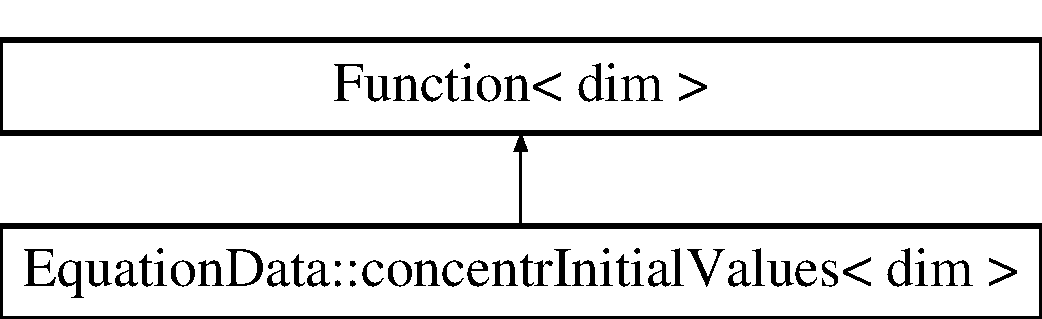
\includegraphics[height=2.000000cm]{class_equation_data_1_1concentr_initial_values}
\end{center}
\end{figure}
\subsubsection*{Public Member Functions}
\begin{DoxyCompactItemize}
\item 
\hyperlink{class_equation_data_1_1concentr_initial_values_a5cb78258be9e0add00e7155fdb7e16e6}{concentr\+Initial\+Values} (double \hyperlink{class_equation_data_1_1concentr_initial_values_a3f0d3b7f4b1d02908f38d83d855718ea}{x})
\item 
virtual double \hyperlink{class_equation_data_1_1concentr_initial_values_a9b67003948ed9e58aece49100f657515}{value} (const Point$<$ dim $>$ \&p, const unsigned int component=0) const 
\item 
virtual void \hyperlink{class_equation_data_1_1concentr_initial_values_a45d0821e98083c9b5dc4b089dc796cb5}{vector\+\_\+value} (const Point$<$ dim $>$ \&p, Vector$<$ double $>$ \&\hyperlink{class_equation_data_1_1concentr_initial_values_a9b67003948ed9e58aece49100f657515}{value}) const 
\item 
virtual void \hyperlink{class_equation_data_1_1concentr_initial_values_a9f23343e83a28890a58ac750ce3379a4}{vector\+\_\+value\+\_\+list} (const std\+::vector$<$ Point$<$ dim $>$ $>$ \&p, std\+::vector$<$ Vector$<$ double $>$ $>$ \&values) const 
\end{DoxyCompactItemize}
\subsubsection*{Public Attributes}
\begin{DoxyCompactItemize}
\item 
double \hyperlink{class_equation_data_1_1concentr_initial_values_a3f0d3b7f4b1d02908f38d83d855718ea}{x}
\end{DoxyCompactItemize}


\subsubsection{Constructor \& Destructor Documentation}
\hypertarget{class_equation_data_1_1concentr_initial_values_a5cb78258be9e0add00e7155fdb7e16e6}{}\index{Equation\+Data\+::concentr\+Initial\+Values@{Equation\+Data\+::concentr\+Initial\+Values}!concentr\+Initial\+Values@{concentr\+Initial\+Values}}
\index{concentr\+Initial\+Values@{concentr\+Initial\+Values}!Equation\+Data\+::concentr\+Initial\+Values@{Equation\+Data\+::concentr\+Initial\+Values}}
\paragraph[{concentr\+Initial\+Values(double x)}]{\setlength{\rightskip}{0pt plus 5cm}template$<$int dim$>$ {\bf Equation\+Data\+::concentr\+Initial\+Values}$<$ dim $>$\+::{\bf concentr\+Initial\+Values} (
\begin{DoxyParamCaption}
\item[{double}]{x}
\end{DoxyParamCaption}
)}\label{class_equation_data_1_1concentr_initial_values_a5cb78258be9e0add00e7155fdb7e16e6}


\subsubsection{Member Function Documentation}
\hypertarget{class_equation_data_1_1concentr_initial_values_a9b67003948ed9e58aece49100f657515}{}\index{Equation\+Data\+::concentr\+Initial\+Values@{Equation\+Data\+::concentr\+Initial\+Values}!value@{value}}
\index{value@{value}!Equation\+Data\+::concentr\+Initial\+Values@{Equation\+Data\+::concentr\+Initial\+Values}}
\paragraph[{value(const Point$<$ dim $>$ \&p, const unsigned int component=0) const }]{\setlength{\rightskip}{0pt plus 5cm}template$<$int dim$>$ double {\bf Equation\+Data\+::concentr\+Initial\+Values}$<$ dim $>$\+::value (
\begin{DoxyParamCaption}
\item[{const Point$<$ dim $>$ \&}]{p, }
\item[{const unsigned int}]{component = {\ttfamily 0}}
\end{DoxyParamCaption}
) const\hspace{0.3cm}{\ttfamily [virtual]}}\label{class_equation_data_1_1concentr_initial_values_a9b67003948ed9e58aece49100f657515}
\hypertarget{class_equation_data_1_1concentr_initial_values_a45d0821e98083c9b5dc4b089dc796cb5}{}\index{Equation\+Data\+::concentr\+Initial\+Values@{Equation\+Data\+::concentr\+Initial\+Values}!vector\+\_\+value@{vector\+\_\+value}}
\index{vector\+\_\+value@{vector\+\_\+value}!Equation\+Data\+::concentr\+Initial\+Values@{Equation\+Data\+::concentr\+Initial\+Values}}
\paragraph[{vector\+\_\+value(const Point$<$ dim $>$ \&p, Vector$<$ double $>$ \&value) const }]{\setlength{\rightskip}{0pt plus 5cm}template$<$int dim$>$ void {\bf Equation\+Data\+::concentr\+Initial\+Values}$<$ dim $>$\+::vector\+\_\+value (
\begin{DoxyParamCaption}
\item[{const Point$<$ dim $>$ \&}]{p, }
\item[{Vector$<$ double $>$ \&}]{value}
\end{DoxyParamCaption}
) const\hspace{0.3cm}{\ttfamily [virtual]}}\label{class_equation_data_1_1concentr_initial_values_a45d0821e98083c9b5dc4b089dc796cb5}
\hypertarget{class_equation_data_1_1concentr_initial_values_a9f23343e83a28890a58ac750ce3379a4}{}\index{Equation\+Data\+::concentr\+Initial\+Values@{Equation\+Data\+::concentr\+Initial\+Values}!vector\+\_\+value\+\_\+list@{vector\+\_\+value\+\_\+list}}
\index{vector\+\_\+value\+\_\+list@{vector\+\_\+value\+\_\+list}!Equation\+Data\+::concentr\+Initial\+Values@{Equation\+Data\+::concentr\+Initial\+Values}}
\paragraph[{vector\+\_\+value\+\_\+list(const std\+::vector$<$ Point$<$ dim $>$ $>$ \&p, std\+::vector$<$ Vector$<$ double $>$ $>$ \&values) const }]{\setlength{\rightskip}{0pt plus 5cm}template$<$int dim$>$ void {\bf Equation\+Data\+::concentr\+Initial\+Values}$<$ dim $>$\+::vector\+\_\+value\+\_\+list (
\begin{DoxyParamCaption}
\item[{const std\+::vector$<$ Point$<$ dim $>$ $>$ \&}]{p, }
\item[{std\+::vector$<$ Vector$<$ double $>$ $>$ \&}]{values}
\end{DoxyParamCaption}
) const\hspace{0.3cm}{\ttfamily [virtual]}}\label{class_equation_data_1_1concentr_initial_values_a9f23343e83a28890a58ac750ce3379a4}


\subsubsection{Member Data Documentation}
\hypertarget{class_equation_data_1_1concentr_initial_values_a3f0d3b7f4b1d02908f38d83d855718ea}{}\index{Equation\+Data\+::concentr\+Initial\+Values@{Equation\+Data\+::concentr\+Initial\+Values}!x@{x}}
\index{x@{x}!Equation\+Data\+::concentr\+Initial\+Values@{Equation\+Data\+::concentr\+Initial\+Values}}
\paragraph[{x}]{\setlength{\rightskip}{0pt plus 5cm}template$<$int dim$>$ double {\bf Equation\+Data\+::concentr\+Initial\+Values}$<$ dim $>$\+::x}\label{class_equation_data_1_1concentr_initial_values_a3f0d3b7f4b1d02908f38d83d855718ea}


The documentation for this class was generated from the following file\+:\begin{DoxyCompactItemize}
\item 
/\+Users/miranus/work/\+Devs/miscible\+\_\+mixing\+\_\+series/miscible\+\_\+mixing/include/mismix/\hyperlink{equation__data_8h}{equation\+\_\+data.\+h}\end{DoxyCompactItemize}

\hypertarget{class_equation_data_1_1concentr_inlet_values}{}\section{Equation\+Data\+:\+:concentr\+Inlet\+Values$<$ dim $>$ Class Template Reference}
\label{class_equation_data_1_1concentr_inlet_values}\index{Equation\+Data\+::concentr\+Inlet\+Values$<$ dim $>$@{Equation\+Data\+::concentr\+Inlet\+Values$<$ dim $>$}}


{\ttfamily \#include $<$equation\+\_\+data.\+h$>$}

Inheritance diagram for Equation\+Data\+:\+:concentr\+Inlet\+Values$<$ dim $>$\+:\begin{figure}[H]
\begin{center}
\leavevmode
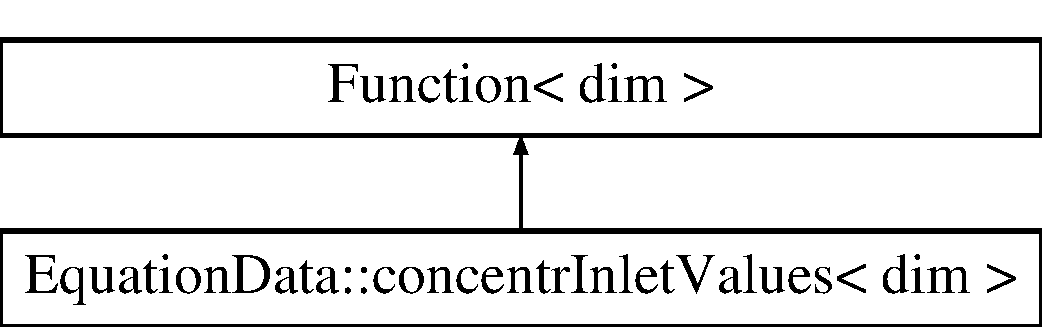
\includegraphics[height=2.000000cm]{class_equation_data_1_1concentr_inlet_values}
\end{center}
\end{figure}
\subsection*{Public Member Functions}
\begin{DoxyCompactItemize}
\item 
\hyperlink{class_equation_data_1_1concentr_inlet_values_a8b12d233a24b1f06625b884c0a649004}{concentr\+Inlet\+Values} ()
\item 
virtual double \hyperlink{class_equation_data_1_1concentr_inlet_values_a819feb903b5bf6afe1aa0ab0f62d31a8}{value} (const Point$<$ dim $>$ \&p, const unsigned int component=0) const 
\item 
virtual void \hyperlink{class_equation_data_1_1concentr_inlet_values_a8b14d66851e8d02b563317ed20ff1a46}{vector\+\_\+value} (const Point$<$ dim $>$ \&p, Vector$<$ double $>$ \&\hyperlink{class_equation_data_1_1concentr_inlet_values_a819feb903b5bf6afe1aa0ab0f62d31a8}{value}) const 
\end{DoxyCompactItemize}


\subsection{Constructor \& Destructor Documentation}
\hypertarget{class_equation_data_1_1concentr_inlet_values_a8b12d233a24b1f06625b884c0a649004}{}\index{Equation\+Data\+::concentr\+Inlet\+Values@{Equation\+Data\+::concentr\+Inlet\+Values}!concentr\+Inlet\+Values@{concentr\+Inlet\+Values}}
\index{concentr\+Inlet\+Values@{concentr\+Inlet\+Values}!Equation\+Data\+::concentr\+Inlet\+Values@{Equation\+Data\+::concentr\+Inlet\+Values}}
\subsubsection[{concentr\+Inlet\+Values()}]{\setlength{\rightskip}{0pt plus 5cm}template$<$int dim$>$ {\bf Equation\+Data\+::concentr\+Inlet\+Values}$<$ dim $>$\+::{\bf concentr\+Inlet\+Values} (
\begin{DoxyParamCaption}
{}
\end{DoxyParamCaption}
)\hspace{0.3cm}{\ttfamily [inline]}}\label{class_equation_data_1_1concentr_inlet_values_a8b12d233a24b1f06625b884c0a649004}


\subsection{Member Function Documentation}
\hypertarget{class_equation_data_1_1concentr_inlet_values_a819feb903b5bf6afe1aa0ab0f62d31a8}{}\index{Equation\+Data\+::concentr\+Inlet\+Values@{Equation\+Data\+::concentr\+Inlet\+Values}!value@{value}}
\index{value@{value}!Equation\+Data\+::concentr\+Inlet\+Values@{Equation\+Data\+::concentr\+Inlet\+Values}}
\subsubsection[{value(const Point$<$ dim $>$ \&p, const unsigned int component=0) const }]{\setlength{\rightskip}{0pt plus 5cm}template$<$int dim$>$ double {\bf Equation\+Data\+::concentr\+Inlet\+Values}$<$ dim $>$\+::value (
\begin{DoxyParamCaption}
\item[{const Point$<$ dim $>$ \&}]{p, }
\item[{const unsigned int}]{component = {\ttfamily 0}}
\end{DoxyParamCaption}
) const\hspace{0.3cm}{\ttfamily [virtual]}}\label{class_equation_data_1_1concentr_inlet_values_a819feb903b5bf6afe1aa0ab0f62d31a8}
\hypertarget{class_equation_data_1_1concentr_inlet_values_a8b14d66851e8d02b563317ed20ff1a46}{}\index{Equation\+Data\+::concentr\+Inlet\+Values@{Equation\+Data\+::concentr\+Inlet\+Values}!vector\+\_\+value@{vector\+\_\+value}}
\index{vector\+\_\+value@{vector\+\_\+value}!Equation\+Data\+::concentr\+Inlet\+Values@{Equation\+Data\+::concentr\+Inlet\+Values}}
\subsubsection[{vector\+\_\+value(const Point$<$ dim $>$ \&p, Vector$<$ double $>$ \&value) const }]{\setlength{\rightskip}{0pt plus 5cm}template$<$int dim$>$ void {\bf Equation\+Data\+::concentr\+Inlet\+Values}$<$ dim $>$\+::vector\+\_\+value (
\begin{DoxyParamCaption}
\item[{const Point$<$ dim $>$ \&}]{p, }
\item[{Vector$<$ double $>$ \&}]{value}
\end{DoxyParamCaption}
) const\hspace{0.3cm}{\ttfamily [virtual]}}\label{class_equation_data_1_1concentr_inlet_values_a8b14d66851e8d02b563317ed20ff1a46}


The documentation for this class was generated from the following file\+:\begin{DoxyCompactItemize}
\item 
/\+Users/miranus/work/\+Devs/miscible\+\_\+mixing\+\_\+series/miscible\+\_\+mixing/include/mismix/\hyperlink{equation__data_8h}{equation\+\_\+data.\+h}\end{DoxyCompactItemize}

\hypertarget{struct_assembly_1_1_scratch_1_1concentr_matrix}{}\section{Assembly\+:\+:Scratch\+:\+:concentr\+Matrix$<$ dim $>$ Struct Template Reference}
\label{struct_assembly_1_1_scratch_1_1concentr_matrix}\index{Assembly\+::\+Scratch\+::concentr\+Matrix$<$ dim $>$@{Assembly\+::\+Scratch\+::concentr\+Matrix$<$ dim $>$}}


{\ttfamily \#include $<$assembly\+\_\+copydata.\+h$>$}

\subsection*{Public Member Functions}
\begin{DoxyCompactItemize}
\item 
\hyperlink{struct_assembly_1_1_scratch_1_1concentr_matrix_a09f4fe4a7e3f71ef4817e9a07b618473}{concentr\+Matrix} (const Finite\+Element$<$ dim $>$ \&concentr\+\_\+fe, const Mapping$<$ dim $>$ \&mapping, const Quadrature$<$ dim $>$ \&concentr\+\_\+quadrature)
\item 
\hyperlink{struct_assembly_1_1_scratch_1_1concentr_matrix_ae04f5cdc68467da262a5c29712790d24}{concentr\+Matrix} (const \hyperlink{struct_assembly_1_1_scratch_1_1concentr_matrix}{concentr\+Matrix} \&data)
\end{DoxyCompactItemize}
\subsection*{Public Attributes}
\begin{DoxyCompactItemize}
\item 
F\+E\+Values$<$ dim $>$ \hyperlink{struct_assembly_1_1_scratch_1_1concentr_matrix_ab33eea0fdd2716aa1aab80e22a3c3d1b}{concentr\+\_\+fe\+\_\+values}
\item 
std\+::vector$<$ double $>$ \hyperlink{struct_assembly_1_1_scratch_1_1concentr_matrix_a66a048dcc5601ac8bf72829c8a2eb567}{phi\+\_\+\+T}
\item 
std\+::vector$<$ Tensor$<$ 1, dim $>$ $>$ \hyperlink{struct_assembly_1_1_scratch_1_1concentr_matrix_a8a597e54b433d76d7e1f71b65b7155e5}{grad\+\_\+phi\+\_\+\+T}
\end{DoxyCompactItemize}


\subsection{Constructor \& Destructor Documentation}
\hypertarget{struct_assembly_1_1_scratch_1_1concentr_matrix_a09f4fe4a7e3f71ef4817e9a07b618473}{}\index{Assembly\+::\+Scratch\+::concentr\+Matrix@{Assembly\+::\+Scratch\+::concentr\+Matrix}!concentr\+Matrix@{concentr\+Matrix}}
\index{concentr\+Matrix@{concentr\+Matrix}!Assembly\+::\+Scratch\+::concentr\+Matrix@{Assembly\+::\+Scratch\+::concentr\+Matrix}}
\subsubsection[{concentr\+Matrix(const Finite\+Element$<$ dim $>$ \&concentr\+\_\+fe, const Mapping$<$ dim $>$ \&mapping, const Quadrature$<$ dim $>$ \&concentr\+\_\+quadrature)}]{\setlength{\rightskip}{0pt plus 5cm}template$<$int dim$>$ {\bf Assembly\+::\+Scratch\+::concentr\+Matrix}$<$ dim $>$\+::{\bf concentr\+Matrix} (
\begin{DoxyParamCaption}
\item[{const Finite\+Element$<$ dim $>$ \&}]{concentr\+\_\+fe, }
\item[{const Mapping$<$ dim $>$ \&}]{mapping, }
\item[{const Quadrature$<$ dim $>$ \&}]{concentr\+\_\+quadrature}
\end{DoxyParamCaption}
)}\label{struct_assembly_1_1_scratch_1_1concentr_matrix_a09f4fe4a7e3f71ef4817e9a07b618473}
\hypertarget{struct_assembly_1_1_scratch_1_1concentr_matrix_ae04f5cdc68467da262a5c29712790d24}{}\index{Assembly\+::\+Scratch\+::concentr\+Matrix@{Assembly\+::\+Scratch\+::concentr\+Matrix}!concentr\+Matrix@{concentr\+Matrix}}
\index{concentr\+Matrix@{concentr\+Matrix}!Assembly\+::\+Scratch\+::concentr\+Matrix@{Assembly\+::\+Scratch\+::concentr\+Matrix}}
\subsubsection[{concentr\+Matrix(const concentr\+Matrix \&data)}]{\setlength{\rightskip}{0pt plus 5cm}template$<$int dim$>$ {\bf Assembly\+::\+Scratch\+::concentr\+Matrix}$<$ dim $>$\+::{\bf concentr\+Matrix} (
\begin{DoxyParamCaption}
\item[{const {\bf concentr\+Matrix}$<$ dim $>$ \&}]{data}
\end{DoxyParamCaption}
)}\label{struct_assembly_1_1_scratch_1_1concentr_matrix_ae04f5cdc68467da262a5c29712790d24}


\subsection{Member Data Documentation}
\hypertarget{struct_assembly_1_1_scratch_1_1concentr_matrix_ab33eea0fdd2716aa1aab80e22a3c3d1b}{}\index{Assembly\+::\+Scratch\+::concentr\+Matrix@{Assembly\+::\+Scratch\+::concentr\+Matrix}!concentr\+\_\+fe\+\_\+values@{concentr\+\_\+fe\+\_\+values}}
\index{concentr\+\_\+fe\+\_\+values@{concentr\+\_\+fe\+\_\+values}!Assembly\+::\+Scratch\+::concentr\+Matrix@{Assembly\+::\+Scratch\+::concentr\+Matrix}}
\subsubsection[{concentr\+\_\+fe\+\_\+values}]{\setlength{\rightskip}{0pt plus 5cm}template$<$int dim$>$ F\+E\+Values$<$dim$>$ {\bf Assembly\+::\+Scratch\+::concentr\+Matrix}$<$ dim $>$\+::concentr\+\_\+fe\+\_\+values}\label{struct_assembly_1_1_scratch_1_1concentr_matrix_ab33eea0fdd2716aa1aab80e22a3c3d1b}
\hypertarget{struct_assembly_1_1_scratch_1_1concentr_matrix_a8a597e54b433d76d7e1f71b65b7155e5}{}\index{Assembly\+::\+Scratch\+::concentr\+Matrix@{Assembly\+::\+Scratch\+::concentr\+Matrix}!grad\+\_\+phi\+\_\+\+T@{grad\+\_\+phi\+\_\+\+T}}
\index{grad\+\_\+phi\+\_\+\+T@{grad\+\_\+phi\+\_\+\+T}!Assembly\+::\+Scratch\+::concentr\+Matrix@{Assembly\+::\+Scratch\+::concentr\+Matrix}}
\subsubsection[{grad\+\_\+phi\+\_\+\+T}]{\setlength{\rightskip}{0pt plus 5cm}template$<$int dim$>$ std\+::vector$<$Tensor$<$1,dim$>$ $>$ {\bf Assembly\+::\+Scratch\+::concentr\+Matrix}$<$ dim $>$\+::grad\+\_\+phi\+\_\+\+T}\label{struct_assembly_1_1_scratch_1_1concentr_matrix_a8a597e54b433d76d7e1f71b65b7155e5}
\hypertarget{struct_assembly_1_1_scratch_1_1concentr_matrix_a66a048dcc5601ac8bf72829c8a2eb567}{}\index{Assembly\+::\+Scratch\+::concentr\+Matrix@{Assembly\+::\+Scratch\+::concentr\+Matrix}!phi\+\_\+\+T@{phi\+\_\+\+T}}
\index{phi\+\_\+\+T@{phi\+\_\+\+T}!Assembly\+::\+Scratch\+::concentr\+Matrix@{Assembly\+::\+Scratch\+::concentr\+Matrix}}
\subsubsection[{phi\+\_\+\+T}]{\setlength{\rightskip}{0pt plus 5cm}template$<$int dim$>$ std\+::vector$<$double$>$ {\bf Assembly\+::\+Scratch\+::concentr\+Matrix}$<$ dim $>$\+::phi\+\_\+\+T}\label{struct_assembly_1_1_scratch_1_1concentr_matrix_a66a048dcc5601ac8bf72829c8a2eb567}


The documentation for this struct was generated from the following file\+:\begin{DoxyCompactItemize}
\item 
/\+Users/miranus/work/\+Devs/miscible\+\_\+mixing\+\_\+series/miscible\+\_\+mixing/include/mismix/\hyperlink{assembly__copydata_8h}{assembly\+\_\+copydata.\+h}\end{DoxyCompactItemize}

\hypertarget{struct_assembly_1_1_copy_data_1_1concentr_matrix}{}\section{Assembly\+:\+:Copy\+Data\+:\+:concentr\+Matrix$<$ dim $>$ Struct Template Reference}
\label{struct_assembly_1_1_copy_data_1_1concentr_matrix}\index{Assembly\+::\+Copy\+Data\+::concentr\+Matrix$<$ dim $>$@{Assembly\+::\+Copy\+Data\+::concentr\+Matrix$<$ dim $>$}}


{\ttfamily \#include $<$assembly\+\_\+copydata.\+h$>$}

\subsection*{Public Member Functions}
\begin{DoxyCompactItemize}
\item 
\hyperlink{struct_assembly_1_1_copy_data_1_1concentr_matrix_a3a79ebd7ee4093e8e06ee9ef0757596a}{concentr\+Matrix} (const Finite\+Element$<$ dim $>$ \&concentr\+\_\+fe)
\item 
\hyperlink{struct_assembly_1_1_copy_data_1_1concentr_matrix_a556e73863e274fc87366b661c0b8c2cb}{concentr\+Matrix} (const \hyperlink{struct_assembly_1_1_copy_data_1_1concentr_matrix}{concentr\+Matrix} \&data)
\end{DoxyCompactItemize}
\subsection*{Public Attributes}
\begin{DoxyCompactItemize}
\item 
Full\+Matrix$<$ double $>$ \hyperlink{struct_assembly_1_1_copy_data_1_1concentr_matrix_ac9d3fa147044cb330edcbfb28c9a51d8}{local\+\_\+mass\+\_\+matrix}
\item 
Full\+Matrix$<$ double $>$ \hyperlink{struct_assembly_1_1_copy_data_1_1concentr_matrix_ae611593ae75fc8317c368c54443a63f8}{local\+\_\+stiffness\+\_\+matrix}
\item 
std\+::vector$<$ types\+::global\+\_\+dof\+\_\+index $>$ \hyperlink{struct_assembly_1_1_copy_data_1_1concentr_matrix_a0388e1a38666197f44bfe6c39d95f6c6}{local\+\_\+dof\+\_\+indices}
\end{DoxyCompactItemize}


\subsection{Constructor \& Destructor Documentation}
\hypertarget{struct_assembly_1_1_copy_data_1_1concentr_matrix_a3a79ebd7ee4093e8e06ee9ef0757596a}{}\index{Assembly\+::\+Copy\+Data\+::concentr\+Matrix@{Assembly\+::\+Copy\+Data\+::concentr\+Matrix}!concentr\+Matrix@{concentr\+Matrix}}
\index{concentr\+Matrix@{concentr\+Matrix}!Assembly\+::\+Copy\+Data\+::concentr\+Matrix@{Assembly\+::\+Copy\+Data\+::concentr\+Matrix}}
\subsubsection[{concentr\+Matrix(const Finite\+Element$<$ dim $>$ \&concentr\+\_\+fe)}]{\setlength{\rightskip}{0pt plus 5cm}template$<$int dim$>$ {\bf Assembly\+::\+Copy\+Data\+::concentr\+Matrix}$<$ dim $>$\+::{\bf concentr\+Matrix} (
\begin{DoxyParamCaption}
\item[{const Finite\+Element$<$ dim $>$ \&}]{concentr\+\_\+fe}
\end{DoxyParamCaption}
)}\label{struct_assembly_1_1_copy_data_1_1concentr_matrix_a3a79ebd7ee4093e8e06ee9ef0757596a}
\hypertarget{struct_assembly_1_1_copy_data_1_1concentr_matrix_a556e73863e274fc87366b661c0b8c2cb}{}\index{Assembly\+::\+Copy\+Data\+::concentr\+Matrix@{Assembly\+::\+Copy\+Data\+::concentr\+Matrix}!concentr\+Matrix@{concentr\+Matrix}}
\index{concentr\+Matrix@{concentr\+Matrix}!Assembly\+::\+Copy\+Data\+::concentr\+Matrix@{Assembly\+::\+Copy\+Data\+::concentr\+Matrix}}
\subsubsection[{concentr\+Matrix(const concentr\+Matrix \&data)}]{\setlength{\rightskip}{0pt plus 5cm}template$<$int dim$>$ {\bf Assembly\+::\+Copy\+Data\+::concentr\+Matrix}$<$ dim $>$\+::{\bf concentr\+Matrix} (
\begin{DoxyParamCaption}
\item[{const {\bf concentr\+Matrix}$<$ dim $>$ \&}]{data}
\end{DoxyParamCaption}
)}\label{struct_assembly_1_1_copy_data_1_1concentr_matrix_a556e73863e274fc87366b661c0b8c2cb}


\subsection{Member Data Documentation}
\hypertarget{struct_assembly_1_1_copy_data_1_1concentr_matrix_a0388e1a38666197f44bfe6c39d95f6c6}{}\index{Assembly\+::\+Copy\+Data\+::concentr\+Matrix@{Assembly\+::\+Copy\+Data\+::concentr\+Matrix}!local\+\_\+dof\+\_\+indices@{local\+\_\+dof\+\_\+indices}}
\index{local\+\_\+dof\+\_\+indices@{local\+\_\+dof\+\_\+indices}!Assembly\+::\+Copy\+Data\+::concentr\+Matrix@{Assembly\+::\+Copy\+Data\+::concentr\+Matrix}}
\subsubsection[{local\+\_\+dof\+\_\+indices}]{\setlength{\rightskip}{0pt plus 5cm}template$<$int dim$>$ std\+::vector$<$types\+::global\+\_\+dof\+\_\+index$>$ {\bf Assembly\+::\+Copy\+Data\+::concentr\+Matrix}$<$ dim $>$\+::local\+\_\+dof\+\_\+indices}\label{struct_assembly_1_1_copy_data_1_1concentr_matrix_a0388e1a38666197f44bfe6c39d95f6c6}
\hypertarget{struct_assembly_1_1_copy_data_1_1concentr_matrix_ac9d3fa147044cb330edcbfb28c9a51d8}{}\index{Assembly\+::\+Copy\+Data\+::concentr\+Matrix@{Assembly\+::\+Copy\+Data\+::concentr\+Matrix}!local\+\_\+mass\+\_\+matrix@{local\+\_\+mass\+\_\+matrix}}
\index{local\+\_\+mass\+\_\+matrix@{local\+\_\+mass\+\_\+matrix}!Assembly\+::\+Copy\+Data\+::concentr\+Matrix@{Assembly\+::\+Copy\+Data\+::concentr\+Matrix}}
\subsubsection[{local\+\_\+mass\+\_\+matrix}]{\setlength{\rightskip}{0pt plus 5cm}template$<$int dim$>$ Full\+Matrix$<$double$>$ {\bf Assembly\+::\+Copy\+Data\+::concentr\+Matrix}$<$ dim $>$\+::local\+\_\+mass\+\_\+matrix}\label{struct_assembly_1_1_copy_data_1_1concentr_matrix_ac9d3fa147044cb330edcbfb28c9a51d8}
\hypertarget{struct_assembly_1_1_copy_data_1_1concentr_matrix_ae611593ae75fc8317c368c54443a63f8}{}\index{Assembly\+::\+Copy\+Data\+::concentr\+Matrix@{Assembly\+::\+Copy\+Data\+::concentr\+Matrix}!local\+\_\+stiffness\+\_\+matrix@{local\+\_\+stiffness\+\_\+matrix}}
\index{local\+\_\+stiffness\+\_\+matrix@{local\+\_\+stiffness\+\_\+matrix}!Assembly\+::\+Copy\+Data\+::concentr\+Matrix@{Assembly\+::\+Copy\+Data\+::concentr\+Matrix}}
\subsubsection[{local\+\_\+stiffness\+\_\+matrix}]{\setlength{\rightskip}{0pt plus 5cm}template$<$int dim$>$ Full\+Matrix$<$double$>$ {\bf Assembly\+::\+Copy\+Data\+::concentr\+Matrix}$<$ dim $>$\+::local\+\_\+stiffness\+\_\+matrix}\label{struct_assembly_1_1_copy_data_1_1concentr_matrix_ae611593ae75fc8317c368c54443a63f8}


The documentation for this struct was generated from the following file\+:\begin{DoxyCompactItemize}
\item 
/\+Users/miranus/work/\+Devs/miscible\+\_\+mixing\+\_\+series/miscible\+\_\+mixing/include/mismix/\hyperlink{assembly__copydata_8h}{assembly\+\_\+copydata.\+h}\end{DoxyCompactItemize}

\hypertarget{struct_assembly_1_1_scratch_1_1concentr_r_h_s}{}\subsection{Assembly\+:\+:Scratch\+:\+:concentr\+R\+H\+S$<$ dim $>$ Struct Template Reference}
\label{struct_assembly_1_1_scratch_1_1concentr_r_h_s}\index{Assembly\+::\+Scratch\+::concentr\+R\+H\+S$<$ dim $>$@{Assembly\+::\+Scratch\+::concentr\+R\+H\+S$<$ dim $>$}}


{\ttfamily \#include $<$assembly\+\_\+copydata.\+h$>$}

\subsubsection*{Public Member Functions}
\begin{DoxyCompactItemize}
\item 
\hyperlink{struct_assembly_1_1_scratch_1_1concentr_r_h_s_af8cd490e71848eda2821fa50503094bc}{concentr\+R\+H\+S} (const Finite\+Element$<$ dim $>$ \&concentr\+\_\+fe, const Finite\+Element$<$ dim $>$ \&fe\+\_\+velocity, const Mapping$<$ dim $>$ \&mapping, const Quadrature$<$ dim $>$ \&quadrature)
\item 
\hyperlink{struct_assembly_1_1_scratch_1_1concentr_r_h_s_a41cd0bab73e9eff227b5f26bd0cf5ac7}{concentr\+R\+H\+S} (const \hyperlink{struct_assembly_1_1_scratch_1_1concentr_r_h_s}{concentr\+R\+H\+S} \&data)
\end{DoxyCompactItemize}
\subsubsection*{Public Attributes}
\begin{DoxyCompactItemize}
\item 
F\+E\+Values$<$ dim $>$ \hyperlink{struct_assembly_1_1_scratch_1_1concentr_r_h_s_a9bc67b73e78fc8615584d194c3b85106}{concentr\+\_\+fe\+\_\+values}
\item 
F\+E\+Values$<$ dim $>$ \hyperlink{struct_assembly_1_1_scratch_1_1concentr_r_h_s_ad2de28d5b653c8ee22e96ea33c32c55a}{fe\+\_\+velocity\+\_\+values}
\item 
std\+::vector$<$ double $>$ \hyperlink{struct_assembly_1_1_scratch_1_1concentr_r_h_s_acba65db7ab7aece30027901e3b0f030a}{phi\+\_\+\+T}
\item 
std\+::vector$<$ Tensor$<$ 1, dim $>$ $>$ \hyperlink{struct_assembly_1_1_scratch_1_1concentr_r_h_s_a6168fae7e16f02fb680dd33d4adf7b3c}{grad\+\_\+phi\+\_\+\+T}
\item 
std\+::vector$<$ Tensor$<$ 1, dim $>$ $>$ \hyperlink{struct_assembly_1_1_scratch_1_1concentr_r_h_s_a387df4b1d77c791fa36096d021da90b0}{old\+\_\+velocity\+\_\+values}
\item 
std\+::vector$<$ Tensor$<$ 1, dim $>$ $>$ \hyperlink{struct_assembly_1_1_scratch_1_1concentr_r_h_s_a7914c7c1d8f2232465ff96be67aecc93}{old\+\_\+old\+\_\+velocity\+\_\+values}
\item 
std\+::vector$<$ Symmetric\+Tensor$<$ 2, dim $>$ $>$ \hyperlink{struct_assembly_1_1_scratch_1_1concentr_r_h_s_ac8bb5dab7eeb953de8020714bf306e0c}{old\+\_\+strain\+\_\+rates}
\item 
std\+::vector$<$ Symmetric\+Tensor$<$ 2, dim $>$ $>$ \hyperlink{struct_assembly_1_1_scratch_1_1concentr_r_h_s_ac722877b3d573cc39c3503a9b2607004}{old\+\_\+old\+\_\+strain\+\_\+rates}
\item 
std\+::vector$<$ double $>$ \hyperlink{struct_assembly_1_1_scratch_1_1concentr_r_h_s_a58249a4ae522e0e939e0260983be8e14}{old\+\_\+concentr\+\_\+values}
\item 
std\+::vector$<$ double $>$ \hyperlink{struct_assembly_1_1_scratch_1_1concentr_r_h_s_ab7f32838f72a67cf1fd4a837d790bae9}{old\+\_\+old\+\_\+concentr\+\_\+values}
\item 
std\+::vector$<$ Tensor$<$ 1, dim $>$ $>$ \hyperlink{struct_assembly_1_1_scratch_1_1concentr_r_h_s_a0b35928e795a32329965539123ffe0fd}{old\+\_\+concentr\+\_\+grads}
\item 
std\+::vector$<$ Tensor$<$ 1, dim $>$ $>$ \hyperlink{struct_assembly_1_1_scratch_1_1concentr_r_h_s_a8604e75641eb86196bda5d51d2d0bc02}{old\+\_\+old\+\_\+concentr\+\_\+grads}
\item 
std\+::vector$<$ double $>$ \hyperlink{struct_assembly_1_1_scratch_1_1concentr_r_h_s_ad65f167402d66f381aa6a847e223efc6}{old\+\_\+concentr\+\_\+laplacians}
\item 
std\+::vector$<$ double $>$ \hyperlink{struct_assembly_1_1_scratch_1_1concentr_r_h_s_a42468e166f46196231a07b524345670a}{old\+\_\+old\+\_\+concentr\+\_\+laplacians}
\end{DoxyCompactItemize}


\subsubsection{Constructor \& Destructor Documentation}
\hypertarget{struct_assembly_1_1_scratch_1_1concentr_r_h_s_af8cd490e71848eda2821fa50503094bc}{}\index{Assembly\+::\+Scratch\+::concentr\+R\+H\+S@{Assembly\+::\+Scratch\+::concentr\+R\+H\+S}!concentr\+R\+H\+S@{concentr\+R\+H\+S}}
\index{concentr\+R\+H\+S@{concentr\+R\+H\+S}!Assembly\+::\+Scratch\+::concentr\+R\+H\+S@{Assembly\+::\+Scratch\+::concentr\+R\+H\+S}}
\paragraph[{concentr\+R\+H\+S(const Finite\+Element$<$ dim $>$ \&concentr\+\_\+fe, const Finite\+Element$<$ dim $>$ \&fe\+\_\+velocity, const Mapping$<$ dim $>$ \&mapping, const Quadrature$<$ dim $>$ \&quadrature)}]{\setlength{\rightskip}{0pt plus 5cm}template$<$int dim$>$ {\bf Assembly\+::\+Scratch\+::concentr\+R\+H\+S}$<$ dim $>$\+::{\bf concentr\+R\+H\+S} (
\begin{DoxyParamCaption}
\item[{const Finite\+Element$<$ dim $>$ \&}]{concentr\+\_\+fe, }
\item[{const Finite\+Element$<$ dim $>$ \&}]{fe\+\_\+velocity, }
\item[{const Mapping$<$ dim $>$ \&}]{mapping, }
\item[{const Quadrature$<$ dim $>$ \&}]{quadrature}
\end{DoxyParamCaption}
)}\label{struct_assembly_1_1_scratch_1_1concentr_r_h_s_af8cd490e71848eda2821fa50503094bc}
\hypertarget{struct_assembly_1_1_scratch_1_1concentr_r_h_s_a41cd0bab73e9eff227b5f26bd0cf5ac7}{}\index{Assembly\+::\+Scratch\+::concentr\+R\+H\+S@{Assembly\+::\+Scratch\+::concentr\+R\+H\+S}!concentr\+R\+H\+S@{concentr\+R\+H\+S}}
\index{concentr\+R\+H\+S@{concentr\+R\+H\+S}!Assembly\+::\+Scratch\+::concentr\+R\+H\+S@{Assembly\+::\+Scratch\+::concentr\+R\+H\+S}}
\paragraph[{concentr\+R\+H\+S(const concentr\+R\+H\+S \&data)}]{\setlength{\rightskip}{0pt plus 5cm}template$<$int dim$>$ {\bf Assembly\+::\+Scratch\+::concentr\+R\+H\+S}$<$ dim $>$\+::{\bf concentr\+R\+H\+S} (
\begin{DoxyParamCaption}
\item[{const {\bf concentr\+R\+H\+S}$<$ dim $>$ \&}]{data}
\end{DoxyParamCaption}
)}\label{struct_assembly_1_1_scratch_1_1concentr_r_h_s_a41cd0bab73e9eff227b5f26bd0cf5ac7}


\subsubsection{Member Data Documentation}
\hypertarget{struct_assembly_1_1_scratch_1_1concentr_r_h_s_a9bc67b73e78fc8615584d194c3b85106}{}\index{Assembly\+::\+Scratch\+::concentr\+R\+H\+S@{Assembly\+::\+Scratch\+::concentr\+R\+H\+S}!concentr\+\_\+fe\+\_\+values@{concentr\+\_\+fe\+\_\+values}}
\index{concentr\+\_\+fe\+\_\+values@{concentr\+\_\+fe\+\_\+values}!Assembly\+::\+Scratch\+::concentr\+R\+H\+S@{Assembly\+::\+Scratch\+::concentr\+R\+H\+S}}
\paragraph[{concentr\+\_\+fe\+\_\+values}]{\setlength{\rightskip}{0pt plus 5cm}template$<$int dim$>$ F\+E\+Values$<$dim$>$ {\bf Assembly\+::\+Scratch\+::concentr\+R\+H\+S}$<$ dim $>$\+::concentr\+\_\+fe\+\_\+values}\label{struct_assembly_1_1_scratch_1_1concentr_r_h_s_a9bc67b73e78fc8615584d194c3b85106}
\hypertarget{struct_assembly_1_1_scratch_1_1concentr_r_h_s_ad2de28d5b653c8ee22e96ea33c32c55a}{}\index{Assembly\+::\+Scratch\+::concentr\+R\+H\+S@{Assembly\+::\+Scratch\+::concentr\+R\+H\+S}!fe\+\_\+velocity\+\_\+values@{fe\+\_\+velocity\+\_\+values}}
\index{fe\+\_\+velocity\+\_\+values@{fe\+\_\+velocity\+\_\+values}!Assembly\+::\+Scratch\+::concentr\+R\+H\+S@{Assembly\+::\+Scratch\+::concentr\+R\+H\+S}}
\paragraph[{fe\+\_\+velocity\+\_\+values}]{\setlength{\rightskip}{0pt plus 5cm}template$<$int dim$>$ F\+E\+Values$<$dim$>$ {\bf Assembly\+::\+Scratch\+::concentr\+R\+H\+S}$<$ dim $>$\+::fe\+\_\+velocity\+\_\+values}\label{struct_assembly_1_1_scratch_1_1concentr_r_h_s_ad2de28d5b653c8ee22e96ea33c32c55a}
\hypertarget{struct_assembly_1_1_scratch_1_1concentr_r_h_s_a6168fae7e16f02fb680dd33d4adf7b3c}{}\index{Assembly\+::\+Scratch\+::concentr\+R\+H\+S@{Assembly\+::\+Scratch\+::concentr\+R\+H\+S}!grad\+\_\+phi\+\_\+\+T@{grad\+\_\+phi\+\_\+\+T}}
\index{grad\+\_\+phi\+\_\+\+T@{grad\+\_\+phi\+\_\+\+T}!Assembly\+::\+Scratch\+::concentr\+R\+H\+S@{Assembly\+::\+Scratch\+::concentr\+R\+H\+S}}
\paragraph[{grad\+\_\+phi\+\_\+\+T}]{\setlength{\rightskip}{0pt plus 5cm}template$<$int dim$>$ std\+::vector$<$Tensor$<$1,dim$>$ $>$ {\bf Assembly\+::\+Scratch\+::concentr\+R\+H\+S}$<$ dim $>$\+::grad\+\_\+phi\+\_\+\+T}\label{struct_assembly_1_1_scratch_1_1concentr_r_h_s_a6168fae7e16f02fb680dd33d4adf7b3c}
\hypertarget{struct_assembly_1_1_scratch_1_1concentr_r_h_s_a0b35928e795a32329965539123ffe0fd}{}\index{Assembly\+::\+Scratch\+::concentr\+R\+H\+S@{Assembly\+::\+Scratch\+::concentr\+R\+H\+S}!old\+\_\+concentr\+\_\+grads@{old\+\_\+concentr\+\_\+grads}}
\index{old\+\_\+concentr\+\_\+grads@{old\+\_\+concentr\+\_\+grads}!Assembly\+::\+Scratch\+::concentr\+R\+H\+S@{Assembly\+::\+Scratch\+::concentr\+R\+H\+S}}
\paragraph[{old\+\_\+concentr\+\_\+grads}]{\setlength{\rightskip}{0pt plus 5cm}template$<$int dim$>$ std\+::vector$<$Tensor$<$1,dim$>$ $>$ {\bf Assembly\+::\+Scratch\+::concentr\+R\+H\+S}$<$ dim $>$\+::old\+\_\+concentr\+\_\+grads}\label{struct_assembly_1_1_scratch_1_1concentr_r_h_s_a0b35928e795a32329965539123ffe0fd}
\hypertarget{struct_assembly_1_1_scratch_1_1concentr_r_h_s_ad65f167402d66f381aa6a847e223efc6}{}\index{Assembly\+::\+Scratch\+::concentr\+R\+H\+S@{Assembly\+::\+Scratch\+::concentr\+R\+H\+S}!old\+\_\+concentr\+\_\+laplacians@{old\+\_\+concentr\+\_\+laplacians}}
\index{old\+\_\+concentr\+\_\+laplacians@{old\+\_\+concentr\+\_\+laplacians}!Assembly\+::\+Scratch\+::concentr\+R\+H\+S@{Assembly\+::\+Scratch\+::concentr\+R\+H\+S}}
\paragraph[{old\+\_\+concentr\+\_\+laplacians}]{\setlength{\rightskip}{0pt plus 5cm}template$<$int dim$>$ std\+::vector$<$double$>$ {\bf Assembly\+::\+Scratch\+::concentr\+R\+H\+S}$<$ dim $>$\+::old\+\_\+concentr\+\_\+laplacians}\label{struct_assembly_1_1_scratch_1_1concentr_r_h_s_ad65f167402d66f381aa6a847e223efc6}
\hypertarget{struct_assembly_1_1_scratch_1_1concentr_r_h_s_a58249a4ae522e0e939e0260983be8e14}{}\index{Assembly\+::\+Scratch\+::concentr\+R\+H\+S@{Assembly\+::\+Scratch\+::concentr\+R\+H\+S}!old\+\_\+concentr\+\_\+values@{old\+\_\+concentr\+\_\+values}}
\index{old\+\_\+concentr\+\_\+values@{old\+\_\+concentr\+\_\+values}!Assembly\+::\+Scratch\+::concentr\+R\+H\+S@{Assembly\+::\+Scratch\+::concentr\+R\+H\+S}}
\paragraph[{old\+\_\+concentr\+\_\+values}]{\setlength{\rightskip}{0pt plus 5cm}template$<$int dim$>$ std\+::vector$<$double$>$ {\bf Assembly\+::\+Scratch\+::concentr\+R\+H\+S}$<$ dim $>$\+::old\+\_\+concentr\+\_\+values}\label{struct_assembly_1_1_scratch_1_1concentr_r_h_s_a58249a4ae522e0e939e0260983be8e14}
\hypertarget{struct_assembly_1_1_scratch_1_1concentr_r_h_s_a8604e75641eb86196bda5d51d2d0bc02}{}\index{Assembly\+::\+Scratch\+::concentr\+R\+H\+S@{Assembly\+::\+Scratch\+::concentr\+R\+H\+S}!old\+\_\+old\+\_\+concentr\+\_\+grads@{old\+\_\+old\+\_\+concentr\+\_\+grads}}
\index{old\+\_\+old\+\_\+concentr\+\_\+grads@{old\+\_\+old\+\_\+concentr\+\_\+grads}!Assembly\+::\+Scratch\+::concentr\+R\+H\+S@{Assembly\+::\+Scratch\+::concentr\+R\+H\+S}}
\paragraph[{old\+\_\+old\+\_\+concentr\+\_\+grads}]{\setlength{\rightskip}{0pt plus 5cm}template$<$int dim$>$ std\+::vector$<$Tensor$<$1,dim$>$ $>$ {\bf Assembly\+::\+Scratch\+::concentr\+R\+H\+S}$<$ dim $>$\+::old\+\_\+old\+\_\+concentr\+\_\+grads}\label{struct_assembly_1_1_scratch_1_1concentr_r_h_s_a8604e75641eb86196bda5d51d2d0bc02}
\hypertarget{struct_assembly_1_1_scratch_1_1concentr_r_h_s_a42468e166f46196231a07b524345670a}{}\index{Assembly\+::\+Scratch\+::concentr\+R\+H\+S@{Assembly\+::\+Scratch\+::concentr\+R\+H\+S}!old\+\_\+old\+\_\+concentr\+\_\+laplacians@{old\+\_\+old\+\_\+concentr\+\_\+laplacians}}
\index{old\+\_\+old\+\_\+concentr\+\_\+laplacians@{old\+\_\+old\+\_\+concentr\+\_\+laplacians}!Assembly\+::\+Scratch\+::concentr\+R\+H\+S@{Assembly\+::\+Scratch\+::concentr\+R\+H\+S}}
\paragraph[{old\+\_\+old\+\_\+concentr\+\_\+laplacians}]{\setlength{\rightskip}{0pt plus 5cm}template$<$int dim$>$ std\+::vector$<$double$>$ {\bf Assembly\+::\+Scratch\+::concentr\+R\+H\+S}$<$ dim $>$\+::old\+\_\+old\+\_\+concentr\+\_\+laplacians}\label{struct_assembly_1_1_scratch_1_1concentr_r_h_s_a42468e166f46196231a07b524345670a}
\hypertarget{struct_assembly_1_1_scratch_1_1concentr_r_h_s_ab7f32838f72a67cf1fd4a837d790bae9}{}\index{Assembly\+::\+Scratch\+::concentr\+R\+H\+S@{Assembly\+::\+Scratch\+::concentr\+R\+H\+S}!old\+\_\+old\+\_\+concentr\+\_\+values@{old\+\_\+old\+\_\+concentr\+\_\+values}}
\index{old\+\_\+old\+\_\+concentr\+\_\+values@{old\+\_\+old\+\_\+concentr\+\_\+values}!Assembly\+::\+Scratch\+::concentr\+R\+H\+S@{Assembly\+::\+Scratch\+::concentr\+R\+H\+S}}
\paragraph[{old\+\_\+old\+\_\+concentr\+\_\+values}]{\setlength{\rightskip}{0pt plus 5cm}template$<$int dim$>$ std\+::vector$<$double$>$ {\bf Assembly\+::\+Scratch\+::concentr\+R\+H\+S}$<$ dim $>$\+::old\+\_\+old\+\_\+concentr\+\_\+values}\label{struct_assembly_1_1_scratch_1_1concentr_r_h_s_ab7f32838f72a67cf1fd4a837d790bae9}
\hypertarget{struct_assembly_1_1_scratch_1_1concentr_r_h_s_ac722877b3d573cc39c3503a9b2607004}{}\index{Assembly\+::\+Scratch\+::concentr\+R\+H\+S@{Assembly\+::\+Scratch\+::concentr\+R\+H\+S}!old\+\_\+old\+\_\+strain\+\_\+rates@{old\+\_\+old\+\_\+strain\+\_\+rates}}
\index{old\+\_\+old\+\_\+strain\+\_\+rates@{old\+\_\+old\+\_\+strain\+\_\+rates}!Assembly\+::\+Scratch\+::concentr\+R\+H\+S@{Assembly\+::\+Scratch\+::concentr\+R\+H\+S}}
\paragraph[{old\+\_\+old\+\_\+strain\+\_\+rates}]{\setlength{\rightskip}{0pt plus 5cm}template$<$int dim$>$ std\+::vector$<$Symmetric\+Tensor$<$2,dim$>$ $>$ {\bf Assembly\+::\+Scratch\+::concentr\+R\+H\+S}$<$ dim $>$\+::old\+\_\+old\+\_\+strain\+\_\+rates}\label{struct_assembly_1_1_scratch_1_1concentr_r_h_s_ac722877b3d573cc39c3503a9b2607004}
\hypertarget{struct_assembly_1_1_scratch_1_1concentr_r_h_s_a7914c7c1d8f2232465ff96be67aecc93}{}\index{Assembly\+::\+Scratch\+::concentr\+R\+H\+S@{Assembly\+::\+Scratch\+::concentr\+R\+H\+S}!old\+\_\+old\+\_\+velocity\+\_\+values@{old\+\_\+old\+\_\+velocity\+\_\+values}}
\index{old\+\_\+old\+\_\+velocity\+\_\+values@{old\+\_\+old\+\_\+velocity\+\_\+values}!Assembly\+::\+Scratch\+::concentr\+R\+H\+S@{Assembly\+::\+Scratch\+::concentr\+R\+H\+S}}
\paragraph[{old\+\_\+old\+\_\+velocity\+\_\+values}]{\setlength{\rightskip}{0pt plus 5cm}template$<$int dim$>$ std\+::vector$<$Tensor$<$1,dim$>$ $>$ {\bf Assembly\+::\+Scratch\+::concentr\+R\+H\+S}$<$ dim $>$\+::old\+\_\+old\+\_\+velocity\+\_\+values}\label{struct_assembly_1_1_scratch_1_1concentr_r_h_s_a7914c7c1d8f2232465ff96be67aecc93}
\hypertarget{struct_assembly_1_1_scratch_1_1concentr_r_h_s_ac8bb5dab7eeb953de8020714bf306e0c}{}\index{Assembly\+::\+Scratch\+::concentr\+R\+H\+S@{Assembly\+::\+Scratch\+::concentr\+R\+H\+S}!old\+\_\+strain\+\_\+rates@{old\+\_\+strain\+\_\+rates}}
\index{old\+\_\+strain\+\_\+rates@{old\+\_\+strain\+\_\+rates}!Assembly\+::\+Scratch\+::concentr\+R\+H\+S@{Assembly\+::\+Scratch\+::concentr\+R\+H\+S}}
\paragraph[{old\+\_\+strain\+\_\+rates}]{\setlength{\rightskip}{0pt plus 5cm}template$<$int dim$>$ std\+::vector$<$Symmetric\+Tensor$<$2,dim$>$ $>$ {\bf Assembly\+::\+Scratch\+::concentr\+R\+H\+S}$<$ dim $>$\+::old\+\_\+strain\+\_\+rates}\label{struct_assembly_1_1_scratch_1_1concentr_r_h_s_ac8bb5dab7eeb953de8020714bf306e0c}
\hypertarget{struct_assembly_1_1_scratch_1_1concentr_r_h_s_a387df4b1d77c791fa36096d021da90b0}{}\index{Assembly\+::\+Scratch\+::concentr\+R\+H\+S@{Assembly\+::\+Scratch\+::concentr\+R\+H\+S}!old\+\_\+velocity\+\_\+values@{old\+\_\+velocity\+\_\+values}}
\index{old\+\_\+velocity\+\_\+values@{old\+\_\+velocity\+\_\+values}!Assembly\+::\+Scratch\+::concentr\+R\+H\+S@{Assembly\+::\+Scratch\+::concentr\+R\+H\+S}}
\paragraph[{old\+\_\+velocity\+\_\+values}]{\setlength{\rightskip}{0pt plus 5cm}template$<$int dim$>$ std\+::vector$<$Tensor$<$1,dim$>$ $>$ {\bf Assembly\+::\+Scratch\+::concentr\+R\+H\+S}$<$ dim $>$\+::old\+\_\+velocity\+\_\+values}\label{struct_assembly_1_1_scratch_1_1concentr_r_h_s_a387df4b1d77c791fa36096d021da90b0}
\hypertarget{struct_assembly_1_1_scratch_1_1concentr_r_h_s_acba65db7ab7aece30027901e3b0f030a}{}\index{Assembly\+::\+Scratch\+::concentr\+R\+H\+S@{Assembly\+::\+Scratch\+::concentr\+R\+H\+S}!phi\+\_\+\+T@{phi\+\_\+\+T}}
\index{phi\+\_\+\+T@{phi\+\_\+\+T}!Assembly\+::\+Scratch\+::concentr\+R\+H\+S@{Assembly\+::\+Scratch\+::concentr\+R\+H\+S}}
\paragraph[{phi\+\_\+\+T}]{\setlength{\rightskip}{0pt plus 5cm}template$<$int dim$>$ std\+::vector$<$double$>$ {\bf Assembly\+::\+Scratch\+::concentr\+R\+H\+S}$<$ dim $>$\+::phi\+\_\+\+T}\label{struct_assembly_1_1_scratch_1_1concentr_r_h_s_acba65db7ab7aece30027901e3b0f030a}


The documentation for this struct was generated from the following file\+:\begin{DoxyCompactItemize}
\item 
/\+Users/miranus/work/\+Devs/miscible\+\_\+mixing\+\_\+series/miscible\+\_\+mixing/include/mismix/\hyperlink{assembly__copydata_8h}{assembly\+\_\+copydata.\+h}\end{DoxyCompactItemize}

\hypertarget{struct_assembly_1_1_copy_data_1_1concentr_r_h_s}{}\subsection{Assembly\+:\+:Copy\+Data\+:\+:concentr\+R\+H\+S$<$ dim $>$ Struct Template Reference}
\label{struct_assembly_1_1_copy_data_1_1concentr_r_h_s}\index{Assembly\+::\+Copy\+Data\+::concentr\+R\+H\+S$<$ dim $>$@{Assembly\+::\+Copy\+Data\+::concentr\+R\+H\+S$<$ dim $>$}}


{\ttfamily \#include $<$assembly\+\_\+copydata.\+h$>$}

\subsubsection*{Public Member Functions}
\begin{DoxyCompactItemize}
\item 
\hyperlink{struct_assembly_1_1_copy_data_1_1concentr_r_h_s_adc0bbc1d0ab17592b775f1f3e10fce99}{concentr\+R\+H\+S} (const Finite\+Element$<$ dim $>$ \&concentr\+\_\+fe)
\item 
\hyperlink{struct_assembly_1_1_copy_data_1_1concentr_r_h_s_a28690ab676550d9de1b9b14f0c92e89b}{concentr\+R\+H\+S} (const \hyperlink{struct_assembly_1_1_copy_data_1_1concentr_r_h_s}{concentr\+R\+H\+S} \&data)
\end{DoxyCompactItemize}
\subsubsection*{Public Attributes}
\begin{DoxyCompactItemize}
\item 
Vector$<$ double $>$ \hyperlink{struct_assembly_1_1_copy_data_1_1concentr_r_h_s_aa16d978b90728b2e6118f642cd012d53}{local\+\_\+rhs}
\item 
std\+::vector$<$ types\+::global\+\_\+dof\+\_\+index $>$ \hyperlink{struct_assembly_1_1_copy_data_1_1concentr_r_h_s_a5e754dc8716eaebaeee1144ad1c59f16}{local\+\_\+dof\+\_\+indices}
\item 
Full\+Matrix$<$ double $>$ \hyperlink{struct_assembly_1_1_copy_data_1_1concentr_r_h_s_af68abcf2cce508ca241f8a57a4160b5d}{matrix\+\_\+for\+\_\+bc}
\end{DoxyCompactItemize}


\subsubsection{Constructor \& Destructor Documentation}
\hypertarget{struct_assembly_1_1_copy_data_1_1concentr_r_h_s_adc0bbc1d0ab17592b775f1f3e10fce99}{}\index{Assembly\+::\+Copy\+Data\+::concentr\+R\+H\+S@{Assembly\+::\+Copy\+Data\+::concentr\+R\+H\+S}!concentr\+R\+H\+S@{concentr\+R\+H\+S}}
\index{concentr\+R\+H\+S@{concentr\+R\+H\+S}!Assembly\+::\+Copy\+Data\+::concentr\+R\+H\+S@{Assembly\+::\+Copy\+Data\+::concentr\+R\+H\+S}}
\paragraph[{concentr\+R\+H\+S(const Finite\+Element$<$ dim $>$ \&concentr\+\_\+fe)}]{\setlength{\rightskip}{0pt plus 5cm}template$<$int dim$>$ {\bf Assembly\+::\+Copy\+Data\+::concentr\+R\+H\+S}$<$ dim $>$\+::{\bf concentr\+R\+H\+S} (
\begin{DoxyParamCaption}
\item[{const Finite\+Element$<$ dim $>$ \&}]{concentr\+\_\+fe}
\end{DoxyParamCaption}
)}\label{struct_assembly_1_1_copy_data_1_1concentr_r_h_s_adc0bbc1d0ab17592b775f1f3e10fce99}
\hypertarget{struct_assembly_1_1_copy_data_1_1concentr_r_h_s_a28690ab676550d9de1b9b14f0c92e89b}{}\index{Assembly\+::\+Copy\+Data\+::concentr\+R\+H\+S@{Assembly\+::\+Copy\+Data\+::concentr\+R\+H\+S}!concentr\+R\+H\+S@{concentr\+R\+H\+S}}
\index{concentr\+R\+H\+S@{concentr\+R\+H\+S}!Assembly\+::\+Copy\+Data\+::concentr\+R\+H\+S@{Assembly\+::\+Copy\+Data\+::concentr\+R\+H\+S}}
\paragraph[{concentr\+R\+H\+S(const concentr\+R\+H\+S \&data)}]{\setlength{\rightskip}{0pt plus 5cm}template$<$int dim$>$ {\bf Assembly\+::\+Copy\+Data\+::concentr\+R\+H\+S}$<$ dim $>$\+::{\bf concentr\+R\+H\+S} (
\begin{DoxyParamCaption}
\item[{const {\bf concentr\+R\+H\+S}$<$ dim $>$ \&}]{data}
\end{DoxyParamCaption}
)}\label{struct_assembly_1_1_copy_data_1_1concentr_r_h_s_a28690ab676550d9de1b9b14f0c92e89b}


\subsubsection{Member Data Documentation}
\hypertarget{struct_assembly_1_1_copy_data_1_1concentr_r_h_s_a5e754dc8716eaebaeee1144ad1c59f16}{}\index{Assembly\+::\+Copy\+Data\+::concentr\+R\+H\+S@{Assembly\+::\+Copy\+Data\+::concentr\+R\+H\+S}!local\+\_\+dof\+\_\+indices@{local\+\_\+dof\+\_\+indices}}
\index{local\+\_\+dof\+\_\+indices@{local\+\_\+dof\+\_\+indices}!Assembly\+::\+Copy\+Data\+::concentr\+R\+H\+S@{Assembly\+::\+Copy\+Data\+::concentr\+R\+H\+S}}
\paragraph[{local\+\_\+dof\+\_\+indices}]{\setlength{\rightskip}{0pt plus 5cm}template$<$int dim$>$ std\+::vector$<$types\+::global\+\_\+dof\+\_\+index$>$ {\bf Assembly\+::\+Copy\+Data\+::concentr\+R\+H\+S}$<$ dim $>$\+::local\+\_\+dof\+\_\+indices}\label{struct_assembly_1_1_copy_data_1_1concentr_r_h_s_a5e754dc8716eaebaeee1144ad1c59f16}
\hypertarget{struct_assembly_1_1_copy_data_1_1concentr_r_h_s_aa16d978b90728b2e6118f642cd012d53}{}\index{Assembly\+::\+Copy\+Data\+::concentr\+R\+H\+S@{Assembly\+::\+Copy\+Data\+::concentr\+R\+H\+S}!local\+\_\+rhs@{local\+\_\+rhs}}
\index{local\+\_\+rhs@{local\+\_\+rhs}!Assembly\+::\+Copy\+Data\+::concentr\+R\+H\+S@{Assembly\+::\+Copy\+Data\+::concentr\+R\+H\+S}}
\paragraph[{local\+\_\+rhs}]{\setlength{\rightskip}{0pt plus 5cm}template$<$int dim$>$ Vector$<$double$>$ {\bf Assembly\+::\+Copy\+Data\+::concentr\+R\+H\+S}$<$ dim $>$\+::local\+\_\+rhs}\label{struct_assembly_1_1_copy_data_1_1concentr_r_h_s_aa16d978b90728b2e6118f642cd012d53}
\hypertarget{struct_assembly_1_1_copy_data_1_1concentr_r_h_s_af68abcf2cce508ca241f8a57a4160b5d}{}\index{Assembly\+::\+Copy\+Data\+::concentr\+R\+H\+S@{Assembly\+::\+Copy\+Data\+::concentr\+R\+H\+S}!matrix\+\_\+for\+\_\+bc@{matrix\+\_\+for\+\_\+bc}}
\index{matrix\+\_\+for\+\_\+bc@{matrix\+\_\+for\+\_\+bc}!Assembly\+::\+Copy\+Data\+::concentr\+R\+H\+S@{Assembly\+::\+Copy\+Data\+::concentr\+R\+H\+S}}
\paragraph[{matrix\+\_\+for\+\_\+bc}]{\setlength{\rightskip}{0pt plus 5cm}template$<$int dim$>$ Full\+Matrix$<$double$>$ {\bf Assembly\+::\+Copy\+Data\+::concentr\+R\+H\+S}$<$ dim $>$\+::matrix\+\_\+for\+\_\+bc}\label{struct_assembly_1_1_copy_data_1_1concentr_r_h_s_af68abcf2cce508ca241f8a57a4160b5d}


The documentation for this struct was generated from the following file\+:\begin{DoxyCompactItemize}
\item 
/\+Users/miranus/work/\+Devs/miscible\+\_\+mixing\+\_\+series/miscible\+\_\+mixing/include/mismix/\hyperlink{assembly__copydata_8h}{assembly\+\_\+copydata.\+h}\end{DoxyCompactItemize}

\hypertarget{struct_assembly_1_1_scratch_1_1diffusion__step}{}\section{Assembly\+:\+:Scratch\+:\+:diffusion\+\_\+step$<$ dim $>$ Struct Template Reference}
\label{struct_assembly_1_1_scratch_1_1diffusion__step}\index{Assembly\+::\+Scratch\+::diffusion\+\_\+step$<$ dim $>$@{Assembly\+::\+Scratch\+::diffusion\+\_\+step$<$ dim $>$}}


{\ttfamily \#include $<$assembly\+\_\+copydata.\+h$>$}

\subsection*{Public Member Functions}
\begin{DoxyCompactItemize}
\item 
\hyperlink{struct_assembly_1_1_scratch_1_1diffusion__step_a5769d06dbf6b99961da088f11f24cce3}{diffusion\+\_\+step} (const Finite\+Element$<$ dim $>$ \&fe\+\_\+velocity, const Mapping$<$ dim $>$ \&velocity\+\_\+mapping, const Quadrature$<$ dim $>$ \&quadrature, const Update\+Flags velocity\+\_\+update\+\_\+flags, const Finite\+Element$<$ dim $>$ \&fe\+\_\+pressure, const Mapping$<$ dim $>$ \&pressure\+\_\+mapping, const Update\+Flags pressure\+\_\+update\+\_\+flags, const Finite\+Element$<$ dim $>$ \&concentr\+\_\+fe, const Mapping$<$ dim $>$ \&concentr\+\_\+mapping, const Update\+Flags concentr\+\_\+update\+\_\+flags)
\item 
\hyperlink{struct_assembly_1_1_scratch_1_1diffusion__step_acd94c7791e03515bef5208066a1a0a26}{diffusion\+\_\+step} (const \hyperlink{struct_assembly_1_1_scratch_1_1diffusion__step}{diffusion\+\_\+step} \&data)
\end{DoxyCompactItemize}
\subsection*{Public Attributes}
\begin{DoxyCompactItemize}
\item 
F\+E\+Values$<$ dim $>$ \hyperlink{struct_assembly_1_1_scratch_1_1diffusion__step_abc801170e70dc1174e7570a16a9c9cef}{fe\+\_\+velocity\+\_\+values}
\item 
F\+E\+Values$<$ dim $>$ \hyperlink{struct_assembly_1_1_scratch_1_1diffusion__step_a8ae6347dd8bec8156be7f56235d7a10f}{fe\+\_\+pressure\+\_\+values}
\item 
F\+E\+Values$<$ dim $>$ \hyperlink{struct_assembly_1_1_scratch_1_1diffusion__step_a419a532515fcf72c1eaad266fb6fe9c8}{concentr\+\_\+fe\+\_\+values}
\item 
std\+::vector$<$ Tensor$<$ 2, dim $>$ $>$ \hyperlink{struct_assembly_1_1_scratch_1_1diffusion__step_a8d840d813840efeef8363b9630714e6d}{grads\+\_\+phi\+\_\+u}
\item 
std\+::vector$<$ Symmetric\+Tensor$<$ 2, dim $>$ $>$ \hyperlink{struct_assembly_1_1_scratch_1_1diffusion__step_a5f7d1700139f21792a1107ede3903cf5}{symm\+\_\+grads\+\_\+phi\+\_\+u}
\item 
std\+::vector$<$ Tensor$<$ 1, dim $>$ $>$ \hyperlink{struct_assembly_1_1_scratch_1_1diffusion__step_a7aeba7bef458d2c451ec2ca3d0ddbd0f}{phi\+\_\+u}
\item 
std\+::vector$<$ Tensor$<$ 1, dim $>$ $>$ \hyperlink{struct_assembly_1_1_scratch_1_1diffusion__step_a78dbb9aa70e10f4e3400a7ea8df0395f}{divergence\+\_\+phi\+\_\+u}
\item 
std\+::vector$<$ Tensor$<$ 1, dim $>$ $>$ \hyperlink{struct_assembly_1_1_scratch_1_1diffusion__step_a94cf958bf7072a08e34291f3b50f2a51}{vel\+\_\+star\+\_\+values}
\item 
std\+::vector$<$ Tensor$<$ 1, dim $>$ $>$ \hyperlink{struct_assembly_1_1_scratch_1_1diffusion__step_a3c69fd1c796447267c5e60b4574b7cd6}{vel\+\_\+n\+\_\+values}
\item 
std\+::vector$<$ Tensor$<$ 1, dim $>$ $>$ \hyperlink{struct_assembly_1_1_scratch_1_1diffusion__step_a9fdda6a8d4c418b53bd1e9c6e03ffc26}{vel\+\_\+n\+\_\+minus\+\_\+1\+\_\+values}
\item 
std\+::vector$<$ Tensor$<$ 2, dim $>$ $>$ \hyperlink{struct_assembly_1_1_scratch_1_1diffusion__step_a63260a19549621cb2c9c737a0a43e3f5}{grad\+\_\+vel\+\_\+star\+\_\+values}
\item 
std\+::vector$<$ Tensor$<$ 1, dim $>$ $>$ \hyperlink{struct_assembly_1_1_scratch_1_1diffusion__step_af7bfee637fae1cadfde75192f16c0684}{laplacian\+\_\+vel\+\_\+star\+\_\+values}
\item 
std\+::vector$<$ Tensor$<$ 1, dim $>$ $>$ \hyperlink{struct_assembly_1_1_scratch_1_1diffusion__step_ab292f23db9b98fbccc85767584d1af32}{grad\+\_\+aux\+\_\+n\+\_\+values}
\item 
std\+::vector$<$ Tensor$<$ 1, dim $>$ $>$ \hyperlink{struct_assembly_1_1_scratch_1_1diffusion__step_aa1bdc6944aab9389b86a40688274fdee}{grad\+\_\+aux\+\_\+n\+\_\+minus\+\_\+1\+\_\+values}
\item 
std\+::vector$<$ Tensor$<$ 1, dim $>$ $>$ \hyperlink{struct_assembly_1_1_scratch_1_1diffusion__step_aa11a441604ebd698e5294c6ab3a1ffaf}{grad\+\_\+pre\+\_\+n\+\_\+values}
\item 
std\+::vector$<$ Tensor$<$ 2, dim $>$ $>$ \hyperlink{struct_assembly_1_1_scratch_1_1diffusion__step_a8bc0709a8e9e4ba5e0f663e134444978}{grad\+\_\+grad\+\_\+aux\+\_\+n\+\_\+values}
\item 
std\+::vector$<$ Tensor$<$ 2, dim $>$ $>$ \hyperlink{struct_assembly_1_1_scratch_1_1diffusion__step_a0bbde8769e9f2cc428d9bf0f810c7227}{grad\+\_\+grad\+\_\+aux\+\_\+n\+\_\+minus\+\_\+1\+\_\+values}
\item 
std\+::vector$<$ Tensor$<$ 2, dim $>$ $>$ \hyperlink{struct_assembly_1_1_scratch_1_1diffusion__step_a64c3cf16bc7cf4fa8972153f93014cb9}{grad\+\_\+grad\+\_\+pre\+\_\+n\+\_\+values}
\item 
std\+::vector$<$ double $>$ \hyperlink{struct_assembly_1_1_scratch_1_1diffusion__step_a3790368f163ebc0f1671baa5b535b018}{aux\+\_\+n\+\_\+values}
\item 
std\+::vector$<$ double $>$ \hyperlink{struct_assembly_1_1_scratch_1_1diffusion__step_a29786a1632b7b97b41219b6e6804924e}{aux\+\_\+n\+\_\+minus\+\_\+1\+\_\+values}
\item 
std\+::vector$<$ double $>$ \hyperlink{struct_assembly_1_1_scratch_1_1diffusion__step_ae1586636fe3416c069fe1efaa51c80f2}{pre\+\_\+n\+\_\+values}
\item 
std\+::vector$<$ double $>$ \hyperlink{struct_assembly_1_1_scratch_1_1diffusion__step_a2ee9059b21d32ee414bdf8eb96d3c451}{concentr\+\_\+values}
\item 
std\+::vector$<$ Symmetric\+Tensor$<$ 2, dim $>$ $>$ \hyperlink{struct_assembly_1_1_scratch_1_1diffusion__step_a368904230be585863ee201beabbc8fb6}{symm\+\_\+grads\+\_\+vel\+\_\+star}
\end{DoxyCompactItemize}


\subsection{Constructor \& Destructor Documentation}
\hypertarget{struct_assembly_1_1_scratch_1_1diffusion__step_a5769d06dbf6b99961da088f11f24cce3}{}\index{Assembly\+::\+Scratch\+::diffusion\+\_\+step@{Assembly\+::\+Scratch\+::diffusion\+\_\+step}!diffusion\+\_\+step@{diffusion\+\_\+step}}
\index{diffusion\+\_\+step@{diffusion\+\_\+step}!Assembly\+::\+Scratch\+::diffusion\+\_\+step@{Assembly\+::\+Scratch\+::diffusion\+\_\+step}}
\subsubsection[{diffusion\+\_\+step(const Finite\+Element$<$ dim $>$ \&fe\+\_\+velocity, const Mapping$<$ dim $>$ \&velocity\+\_\+mapping, const Quadrature$<$ dim $>$ \&quadrature, const Update\+Flags velocity\+\_\+update\+\_\+flags, const Finite\+Element$<$ dim $>$ \&fe\+\_\+pressure, const Mapping$<$ dim $>$ \&pressure\+\_\+mapping, const Update\+Flags pressure\+\_\+update\+\_\+flags, const Finite\+Element$<$ dim $>$ \&concentr\+\_\+fe, const Mapping$<$ dim $>$ \&concentr\+\_\+mapping, const Update\+Flags concentr\+\_\+update\+\_\+flags)}]{\setlength{\rightskip}{0pt plus 5cm}template$<$int dim$>$ {\bf Assembly\+::\+Scratch\+::diffusion\+\_\+step}$<$ dim $>$\+::{\bf diffusion\+\_\+step} (
\begin{DoxyParamCaption}
\item[{const Finite\+Element$<$ dim $>$ \&}]{fe\+\_\+velocity, }
\item[{const Mapping$<$ dim $>$ \&}]{velocity\+\_\+mapping, }
\item[{const Quadrature$<$ dim $>$ \&}]{quadrature, }
\item[{const Update\+Flags}]{velocity\+\_\+update\+\_\+flags, }
\item[{const Finite\+Element$<$ dim $>$ \&}]{fe\+\_\+pressure, }
\item[{const Mapping$<$ dim $>$ \&}]{pressure\+\_\+mapping, }
\item[{const Update\+Flags}]{pressure\+\_\+update\+\_\+flags, }
\item[{const Finite\+Element$<$ dim $>$ \&}]{concentr\+\_\+fe, }
\item[{const Mapping$<$ dim $>$ \&}]{concentr\+\_\+mapping, }
\item[{const Update\+Flags}]{concentr\+\_\+update\+\_\+flags}
\end{DoxyParamCaption}
)}\label{struct_assembly_1_1_scratch_1_1diffusion__step_a5769d06dbf6b99961da088f11f24cce3}
\hypertarget{struct_assembly_1_1_scratch_1_1diffusion__step_acd94c7791e03515bef5208066a1a0a26}{}\index{Assembly\+::\+Scratch\+::diffusion\+\_\+step@{Assembly\+::\+Scratch\+::diffusion\+\_\+step}!diffusion\+\_\+step@{diffusion\+\_\+step}}
\index{diffusion\+\_\+step@{diffusion\+\_\+step}!Assembly\+::\+Scratch\+::diffusion\+\_\+step@{Assembly\+::\+Scratch\+::diffusion\+\_\+step}}
\subsubsection[{diffusion\+\_\+step(const diffusion\+\_\+step \&data)}]{\setlength{\rightskip}{0pt plus 5cm}template$<$int dim$>$ {\bf Assembly\+::\+Scratch\+::diffusion\+\_\+step}$<$ dim $>$\+::{\bf diffusion\+\_\+step} (
\begin{DoxyParamCaption}
\item[{const {\bf diffusion\+\_\+step}$<$ dim $>$ \&}]{data}
\end{DoxyParamCaption}
)}\label{struct_assembly_1_1_scratch_1_1diffusion__step_acd94c7791e03515bef5208066a1a0a26}


\subsection{Member Data Documentation}
\hypertarget{struct_assembly_1_1_scratch_1_1diffusion__step_a29786a1632b7b97b41219b6e6804924e}{}\index{Assembly\+::\+Scratch\+::diffusion\+\_\+step@{Assembly\+::\+Scratch\+::diffusion\+\_\+step}!aux\+\_\+n\+\_\+minus\+\_\+1\+\_\+values@{aux\+\_\+n\+\_\+minus\+\_\+1\+\_\+values}}
\index{aux\+\_\+n\+\_\+minus\+\_\+1\+\_\+values@{aux\+\_\+n\+\_\+minus\+\_\+1\+\_\+values}!Assembly\+::\+Scratch\+::diffusion\+\_\+step@{Assembly\+::\+Scratch\+::diffusion\+\_\+step}}
\subsubsection[{aux\+\_\+n\+\_\+minus\+\_\+1\+\_\+values}]{\setlength{\rightskip}{0pt plus 5cm}template$<$int dim$>$ std\+::vector$<$double$>$ {\bf Assembly\+::\+Scratch\+::diffusion\+\_\+step}$<$ dim $>$\+::aux\+\_\+n\+\_\+minus\+\_\+1\+\_\+values}\label{struct_assembly_1_1_scratch_1_1diffusion__step_a29786a1632b7b97b41219b6e6804924e}
\hypertarget{struct_assembly_1_1_scratch_1_1diffusion__step_a3790368f163ebc0f1671baa5b535b018}{}\index{Assembly\+::\+Scratch\+::diffusion\+\_\+step@{Assembly\+::\+Scratch\+::diffusion\+\_\+step}!aux\+\_\+n\+\_\+values@{aux\+\_\+n\+\_\+values}}
\index{aux\+\_\+n\+\_\+values@{aux\+\_\+n\+\_\+values}!Assembly\+::\+Scratch\+::diffusion\+\_\+step@{Assembly\+::\+Scratch\+::diffusion\+\_\+step}}
\subsubsection[{aux\+\_\+n\+\_\+values}]{\setlength{\rightskip}{0pt plus 5cm}template$<$int dim$>$ std\+::vector$<$double$>$ {\bf Assembly\+::\+Scratch\+::diffusion\+\_\+step}$<$ dim $>$\+::aux\+\_\+n\+\_\+values}\label{struct_assembly_1_1_scratch_1_1diffusion__step_a3790368f163ebc0f1671baa5b535b018}
\hypertarget{struct_assembly_1_1_scratch_1_1diffusion__step_a419a532515fcf72c1eaad266fb6fe9c8}{}\index{Assembly\+::\+Scratch\+::diffusion\+\_\+step@{Assembly\+::\+Scratch\+::diffusion\+\_\+step}!concentr\+\_\+fe\+\_\+values@{concentr\+\_\+fe\+\_\+values}}
\index{concentr\+\_\+fe\+\_\+values@{concentr\+\_\+fe\+\_\+values}!Assembly\+::\+Scratch\+::diffusion\+\_\+step@{Assembly\+::\+Scratch\+::diffusion\+\_\+step}}
\subsubsection[{concentr\+\_\+fe\+\_\+values}]{\setlength{\rightskip}{0pt plus 5cm}template$<$int dim$>$ F\+E\+Values$<$dim$>$ {\bf Assembly\+::\+Scratch\+::diffusion\+\_\+step}$<$ dim $>$\+::concentr\+\_\+fe\+\_\+values}\label{struct_assembly_1_1_scratch_1_1diffusion__step_a419a532515fcf72c1eaad266fb6fe9c8}
\hypertarget{struct_assembly_1_1_scratch_1_1diffusion__step_a2ee9059b21d32ee414bdf8eb96d3c451}{}\index{Assembly\+::\+Scratch\+::diffusion\+\_\+step@{Assembly\+::\+Scratch\+::diffusion\+\_\+step}!concentr\+\_\+values@{concentr\+\_\+values}}
\index{concentr\+\_\+values@{concentr\+\_\+values}!Assembly\+::\+Scratch\+::diffusion\+\_\+step@{Assembly\+::\+Scratch\+::diffusion\+\_\+step}}
\subsubsection[{concentr\+\_\+values}]{\setlength{\rightskip}{0pt plus 5cm}template$<$int dim$>$ std\+::vector$<$double$>$ {\bf Assembly\+::\+Scratch\+::diffusion\+\_\+step}$<$ dim $>$\+::concentr\+\_\+values}\label{struct_assembly_1_1_scratch_1_1diffusion__step_a2ee9059b21d32ee414bdf8eb96d3c451}
\hypertarget{struct_assembly_1_1_scratch_1_1diffusion__step_a78dbb9aa70e10f4e3400a7ea8df0395f}{}\index{Assembly\+::\+Scratch\+::diffusion\+\_\+step@{Assembly\+::\+Scratch\+::diffusion\+\_\+step}!divergence\+\_\+phi\+\_\+u@{divergence\+\_\+phi\+\_\+u}}
\index{divergence\+\_\+phi\+\_\+u@{divergence\+\_\+phi\+\_\+u}!Assembly\+::\+Scratch\+::diffusion\+\_\+step@{Assembly\+::\+Scratch\+::diffusion\+\_\+step}}
\subsubsection[{divergence\+\_\+phi\+\_\+u}]{\setlength{\rightskip}{0pt plus 5cm}template$<$int dim$>$ std\+::vector$<$Tensor$<$1,dim$>$ $>$ {\bf Assembly\+::\+Scratch\+::diffusion\+\_\+step}$<$ dim $>$\+::divergence\+\_\+phi\+\_\+u}\label{struct_assembly_1_1_scratch_1_1diffusion__step_a78dbb9aa70e10f4e3400a7ea8df0395f}
\hypertarget{struct_assembly_1_1_scratch_1_1diffusion__step_a8ae6347dd8bec8156be7f56235d7a10f}{}\index{Assembly\+::\+Scratch\+::diffusion\+\_\+step@{Assembly\+::\+Scratch\+::diffusion\+\_\+step}!fe\+\_\+pressure\+\_\+values@{fe\+\_\+pressure\+\_\+values}}
\index{fe\+\_\+pressure\+\_\+values@{fe\+\_\+pressure\+\_\+values}!Assembly\+::\+Scratch\+::diffusion\+\_\+step@{Assembly\+::\+Scratch\+::diffusion\+\_\+step}}
\subsubsection[{fe\+\_\+pressure\+\_\+values}]{\setlength{\rightskip}{0pt plus 5cm}template$<$int dim$>$ F\+E\+Values$<$dim$>$ {\bf Assembly\+::\+Scratch\+::diffusion\+\_\+step}$<$ dim $>$\+::fe\+\_\+pressure\+\_\+values}\label{struct_assembly_1_1_scratch_1_1diffusion__step_a8ae6347dd8bec8156be7f56235d7a10f}
\hypertarget{struct_assembly_1_1_scratch_1_1diffusion__step_abc801170e70dc1174e7570a16a9c9cef}{}\index{Assembly\+::\+Scratch\+::diffusion\+\_\+step@{Assembly\+::\+Scratch\+::diffusion\+\_\+step}!fe\+\_\+velocity\+\_\+values@{fe\+\_\+velocity\+\_\+values}}
\index{fe\+\_\+velocity\+\_\+values@{fe\+\_\+velocity\+\_\+values}!Assembly\+::\+Scratch\+::diffusion\+\_\+step@{Assembly\+::\+Scratch\+::diffusion\+\_\+step}}
\subsubsection[{fe\+\_\+velocity\+\_\+values}]{\setlength{\rightskip}{0pt plus 5cm}template$<$int dim$>$ F\+E\+Values$<$dim$>$ {\bf Assembly\+::\+Scratch\+::diffusion\+\_\+step}$<$ dim $>$\+::fe\+\_\+velocity\+\_\+values}\label{struct_assembly_1_1_scratch_1_1diffusion__step_abc801170e70dc1174e7570a16a9c9cef}
\hypertarget{struct_assembly_1_1_scratch_1_1diffusion__step_aa1bdc6944aab9389b86a40688274fdee}{}\index{Assembly\+::\+Scratch\+::diffusion\+\_\+step@{Assembly\+::\+Scratch\+::diffusion\+\_\+step}!grad\+\_\+aux\+\_\+n\+\_\+minus\+\_\+1\+\_\+values@{grad\+\_\+aux\+\_\+n\+\_\+minus\+\_\+1\+\_\+values}}
\index{grad\+\_\+aux\+\_\+n\+\_\+minus\+\_\+1\+\_\+values@{grad\+\_\+aux\+\_\+n\+\_\+minus\+\_\+1\+\_\+values}!Assembly\+::\+Scratch\+::diffusion\+\_\+step@{Assembly\+::\+Scratch\+::diffusion\+\_\+step}}
\subsubsection[{grad\+\_\+aux\+\_\+n\+\_\+minus\+\_\+1\+\_\+values}]{\setlength{\rightskip}{0pt plus 5cm}template$<$int dim$>$ std\+::vector$<$Tensor$<$1,dim$>$ $>$ {\bf Assembly\+::\+Scratch\+::diffusion\+\_\+step}$<$ dim $>$\+::grad\+\_\+aux\+\_\+n\+\_\+minus\+\_\+1\+\_\+values}\label{struct_assembly_1_1_scratch_1_1diffusion__step_aa1bdc6944aab9389b86a40688274fdee}
\hypertarget{struct_assembly_1_1_scratch_1_1diffusion__step_ab292f23db9b98fbccc85767584d1af32}{}\index{Assembly\+::\+Scratch\+::diffusion\+\_\+step@{Assembly\+::\+Scratch\+::diffusion\+\_\+step}!grad\+\_\+aux\+\_\+n\+\_\+values@{grad\+\_\+aux\+\_\+n\+\_\+values}}
\index{grad\+\_\+aux\+\_\+n\+\_\+values@{grad\+\_\+aux\+\_\+n\+\_\+values}!Assembly\+::\+Scratch\+::diffusion\+\_\+step@{Assembly\+::\+Scratch\+::diffusion\+\_\+step}}
\subsubsection[{grad\+\_\+aux\+\_\+n\+\_\+values}]{\setlength{\rightskip}{0pt plus 5cm}template$<$int dim$>$ std\+::vector$<$Tensor$<$1,dim$>$ $>$ {\bf Assembly\+::\+Scratch\+::diffusion\+\_\+step}$<$ dim $>$\+::grad\+\_\+aux\+\_\+n\+\_\+values}\label{struct_assembly_1_1_scratch_1_1diffusion__step_ab292f23db9b98fbccc85767584d1af32}
\hypertarget{struct_assembly_1_1_scratch_1_1diffusion__step_a0bbde8769e9f2cc428d9bf0f810c7227}{}\index{Assembly\+::\+Scratch\+::diffusion\+\_\+step@{Assembly\+::\+Scratch\+::diffusion\+\_\+step}!grad\+\_\+grad\+\_\+aux\+\_\+n\+\_\+minus\+\_\+1\+\_\+values@{grad\+\_\+grad\+\_\+aux\+\_\+n\+\_\+minus\+\_\+1\+\_\+values}}
\index{grad\+\_\+grad\+\_\+aux\+\_\+n\+\_\+minus\+\_\+1\+\_\+values@{grad\+\_\+grad\+\_\+aux\+\_\+n\+\_\+minus\+\_\+1\+\_\+values}!Assembly\+::\+Scratch\+::diffusion\+\_\+step@{Assembly\+::\+Scratch\+::diffusion\+\_\+step}}
\subsubsection[{grad\+\_\+grad\+\_\+aux\+\_\+n\+\_\+minus\+\_\+1\+\_\+values}]{\setlength{\rightskip}{0pt plus 5cm}template$<$int dim$>$ std\+::vector$<$Tensor$<$2,dim$>$ $>$ {\bf Assembly\+::\+Scratch\+::diffusion\+\_\+step}$<$ dim $>$\+::grad\+\_\+grad\+\_\+aux\+\_\+n\+\_\+minus\+\_\+1\+\_\+values}\label{struct_assembly_1_1_scratch_1_1diffusion__step_a0bbde8769e9f2cc428d9bf0f810c7227}
\hypertarget{struct_assembly_1_1_scratch_1_1diffusion__step_a8bc0709a8e9e4ba5e0f663e134444978}{}\index{Assembly\+::\+Scratch\+::diffusion\+\_\+step@{Assembly\+::\+Scratch\+::diffusion\+\_\+step}!grad\+\_\+grad\+\_\+aux\+\_\+n\+\_\+values@{grad\+\_\+grad\+\_\+aux\+\_\+n\+\_\+values}}
\index{grad\+\_\+grad\+\_\+aux\+\_\+n\+\_\+values@{grad\+\_\+grad\+\_\+aux\+\_\+n\+\_\+values}!Assembly\+::\+Scratch\+::diffusion\+\_\+step@{Assembly\+::\+Scratch\+::diffusion\+\_\+step}}
\subsubsection[{grad\+\_\+grad\+\_\+aux\+\_\+n\+\_\+values}]{\setlength{\rightskip}{0pt plus 5cm}template$<$int dim$>$ std\+::vector$<$Tensor$<$2,dim$>$ $>$ {\bf Assembly\+::\+Scratch\+::diffusion\+\_\+step}$<$ dim $>$\+::grad\+\_\+grad\+\_\+aux\+\_\+n\+\_\+values}\label{struct_assembly_1_1_scratch_1_1diffusion__step_a8bc0709a8e9e4ba5e0f663e134444978}
\hypertarget{struct_assembly_1_1_scratch_1_1diffusion__step_a64c3cf16bc7cf4fa8972153f93014cb9}{}\index{Assembly\+::\+Scratch\+::diffusion\+\_\+step@{Assembly\+::\+Scratch\+::diffusion\+\_\+step}!grad\+\_\+grad\+\_\+pre\+\_\+n\+\_\+values@{grad\+\_\+grad\+\_\+pre\+\_\+n\+\_\+values}}
\index{grad\+\_\+grad\+\_\+pre\+\_\+n\+\_\+values@{grad\+\_\+grad\+\_\+pre\+\_\+n\+\_\+values}!Assembly\+::\+Scratch\+::diffusion\+\_\+step@{Assembly\+::\+Scratch\+::diffusion\+\_\+step}}
\subsubsection[{grad\+\_\+grad\+\_\+pre\+\_\+n\+\_\+values}]{\setlength{\rightskip}{0pt plus 5cm}template$<$int dim$>$ std\+::vector$<$Tensor$<$2,dim$>$ $>$ {\bf Assembly\+::\+Scratch\+::diffusion\+\_\+step}$<$ dim $>$\+::grad\+\_\+grad\+\_\+pre\+\_\+n\+\_\+values}\label{struct_assembly_1_1_scratch_1_1diffusion__step_a64c3cf16bc7cf4fa8972153f93014cb9}
\hypertarget{struct_assembly_1_1_scratch_1_1diffusion__step_aa11a441604ebd698e5294c6ab3a1ffaf}{}\index{Assembly\+::\+Scratch\+::diffusion\+\_\+step@{Assembly\+::\+Scratch\+::diffusion\+\_\+step}!grad\+\_\+pre\+\_\+n\+\_\+values@{grad\+\_\+pre\+\_\+n\+\_\+values}}
\index{grad\+\_\+pre\+\_\+n\+\_\+values@{grad\+\_\+pre\+\_\+n\+\_\+values}!Assembly\+::\+Scratch\+::diffusion\+\_\+step@{Assembly\+::\+Scratch\+::diffusion\+\_\+step}}
\subsubsection[{grad\+\_\+pre\+\_\+n\+\_\+values}]{\setlength{\rightskip}{0pt plus 5cm}template$<$int dim$>$ std\+::vector$<$Tensor$<$1,dim$>$ $>$ {\bf Assembly\+::\+Scratch\+::diffusion\+\_\+step}$<$ dim $>$\+::grad\+\_\+pre\+\_\+n\+\_\+values}\label{struct_assembly_1_1_scratch_1_1diffusion__step_aa11a441604ebd698e5294c6ab3a1ffaf}
\hypertarget{struct_assembly_1_1_scratch_1_1diffusion__step_a63260a19549621cb2c9c737a0a43e3f5}{}\index{Assembly\+::\+Scratch\+::diffusion\+\_\+step@{Assembly\+::\+Scratch\+::diffusion\+\_\+step}!grad\+\_\+vel\+\_\+star\+\_\+values@{grad\+\_\+vel\+\_\+star\+\_\+values}}
\index{grad\+\_\+vel\+\_\+star\+\_\+values@{grad\+\_\+vel\+\_\+star\+\_\+values}!Assembly\+::\+Scratch\+::diffusion\+\_\+step@{Assembly\+::\+Scratch\+::diffusion\+\_\+step}}
\subsubsection[{grad\+\_\+vel\+\_\+star\+\_\+values}]{\setlength{\rightskip}{0pt plus 5cm}template$<$int dim$>$ std\+::vector$<$Tensor$<$2,dim$>$ $>$ {\bf Assembly\+::\+Scratch\+::diffusion\+\_\+step}$<$ dim $>$\+::grad\+\_\+vel\+\_\+star\+\_\+values}\label{struct_assembly_1_1_scratch_1_1diffusion__step_a63260a19549621cb2c9c737a0a43e3f5}
\hypertarget{struct_assembly_1_1_scratch_1_1diffusion__step_a8d840d813840efeef8363b9630714e6d}{}\index{Assembly\+::\+Scratch\+::diffusion\+\_\+step@{Assembly\+::\+Scratch\+::diffusion\+\_\+step}!grads\+\_\+phi\+\_\+u@{grads\+\_\+phi\+\_\+u}}
\index{grads\+\_\+phi\+\_\+u@{grads\+\_\+phi\+\_\+u}!Assembly\+::\+Scratch\+::diffusion\+\_\+step@{Assembly\+::\+Scratch\+::diffusion\+\_\+step}}
\subsubsection[{grads\+\_\+phi\+\_\+u}]{\setlength{\rightskip}{0pt plus 5cm}template$<$int dim$>$ std\+::vector$<$Tensor$<$2,dim$>$ $>$ {\bf Assembly\+::\+Scratch\+::diffusion\+\_\+step}$<$ dim $>$\+::grads\+\_\+phi\+\_\+u}\label{struct_assembly_1_1_scratch_1_1diffusion__step_a8d840d813840efeef8363b9630714e6d}
\hypertarget{struct_assembly_1_1_scratch_1_1diffusion__step_af7bfee637fae1cadfde75192f16c0684}{}\index{Assembly\+::\+Scratch\+::diffusion\+\_\+step@{Assembly\+::\+Scratch\+::diffusion\+\_\+step}!laplacian\+\_\+vel\+\_\+star\+\_\+values@{laplacian\+\_\+vel\+\_\+star\+\_\+values}}
\index{laplacian\+\_\+vel\+\_\+star\+\_\+values@{laplacian\+\_\+vel\+\_\+star\+\_\+values}!Assembly\+::\+Scratch\+::diffusion\+\_\+step@{Assembly\+::\+Scratch\+::diffusion\+\_\+step}}
\subsubsection[{laplacian\+\_\+vel\+\_\+star\+\_\+values}]{\setlength{\rightskip}{0pt plus 5cm}template$<$int dim$>$ std\+::vector$<$Tensor$<$1,dim$>$ $>$ {\bf Assembly\+::\+Scratch\+::diffusion\+\_\+step}$<$ dim $>$\+::laplacian\+\_\+vel\+\_\+star\+\_\+values}\label{struct_assembly_1_1_scratch_1_1diffusion__step_af7bfee637fae1cadfde75192f16c0684}
\hypertarget{struct_assembly_1_1_scratch_1_1diffusion__step_a7aeba7bef458d2c451ec2ca3d0ddbd0f}{}\index{Assembly\+::\+Scratch\+::diffusion\+\_\+step@{Assembly\+::\+Scratch\+::diffusion\+\_\+step}!phi\+\_\+u@{phi\+\_\+u}}
\index{phi\+\_\+u@{phi\+\_\+u}!Assembly\+::\+Scratch\+::diffusion\+\_\+step@{Assembly\+::\+Scratch\+::diffusion\+\_\+step}}
\subsubsection[{phi\+\_\+u}]{\setlength{\rightskip}{0pt plus 5cm}template$<$int dim$>$ std\+::vector$<$Tensor$<$1,dim$>$ $>$ {\bf Assembly\+::\+Scratch\+::diffusion\+\_\+step}$<$ dim $>$\+::phi\+\_\+u}\label{struct_assembly_1_1_scratch_1_1diffusion__step_a7aeba7bef458d2c451ec2ca3d0ddbd0f}
\hypertarget{struct_assembly_1_1_scratch_1_1diffusion__step_ae1586636fe3416c069fe1efaa51c80f2}{}\index{Assembly\+::\+Scratch\+::diffusion\+\_\+step@{Assembly\+::\+Scratch\+::diffusion\+\_\+step}!pre\+\_\+n\+\_\+values@{pre\+\_\+n\+\_\+values}}
\index{pre\+\_\+n\+\_\+values@{pre\+\_\+n\+\_\+values}!Assembly\+::\+Scratch\+::diffusion\+\_\+step@{Assembly\+::\+Scratch\+::diffusion\+\_\+step}}
\subsubsection[{pre\+\_\+n\+\_\+values}]{\setlength{\rightskip}{0pt plus 5cm}template$<$int dim$>$ std\+::vector$<$double$>$ {\bf Assembly\+::\+Scratch\+::diffusion\+\_\+step}$<$ dim $>$\+::pre\+\_\+n\+\_\+values}\label{struct_assembly_1_1_scratch_1_1diffusion__step_ae1586636fe3416c069fe1efaa51c80f2}
\hypertarget{struct_assembly_1_1_scratch_1_1diffusion__step_a5f7d1700139f21792a1107ede3903cf5}{}\index{Assembly\+::\+Scratch\+::diffusion\+\_\+step@{Assembly\+::\+Scratch\+::diffusion\+\_\+step}!symm\+\_\+grads\+\_\+phi\+\_\+u@{symm\+\_\+grads\+\_\+phi\+\_\+u}}
\index{symm\+\_\+grads\+\_\+phi\+\_\+u@{symm\+\_\+grads\+\_\+phi\+\_\+u}!Assembly\+::\+Scratch\+::diffusion\+\_\+step@{Assembly\+::\+Scratch\+::diffusion\+\_\+step}}
\subsubsection[{symm\+\_\+grads\+\_\+phi\+\_\+u}]{\setlength{\rightskip}{0pt plus 5cm}template$<$int dim$>$ std\+::vector$<$Symmetric\+Tensor$<$2,dim$>$ $>$ {\bf Assembly\+::\+Scratch\+::diffusion\+\_\+step}$<$ dim $>$\+::symm\+\_\+grads\+\_\+phi\+\_\+u}\label{struct_assembly_1_1_scratch_1_1diffusion__step_a5f7d1700139f21792a1107ede3903cf5}
\hypertarget{struct_assembly_1_1_scratch_1_1diffusion__step_a368904230be585863ee201beabbc8fb6}{}\index{Assembly\+::\+Scratch\+::diffusion\+\_\+step@{Assembly\+::\+Scratch\+::diffusion\+\_\+step}!symm\+\_\+grads\+\_\+vel\+\_\+star@{symm\+\_\+grads\+\_\+vel\+\_\+star}}
\index{symm\+\_\+grads\+\_\+vel\+\_\+star@{symm\+\_\+grads\+\_\+vel\+\_\+star}!Assembly\+::\+Scratch\+::diffusion\+\_\+step@{Assembly\+::\+Scratch\+::diffusion\+\_\+step}}
\subsubsection[{symm\+\_\+grads\+\_\+vel\+\_\+star}]{\setlength{\rightskip}{0pt plus 5cm}template$<$int dim$>$ std\+::vector$<$Symmetric\+Tensor$<$2,dim$>$ $>$ {\bf Assembly\+::\+Scratch\+::diffusion\+\_\+step}$<$ dim $>$\+::symm\+\_\+grads\+\_\+vel\+\_\+star}\label{struct_assembly_1_1_scratch_1_1diffusion__step_a368904230be585863ee201beabbc8fb6}
\hypertarget{struct_assembly_1_1_scratch_1_1diffusion__step_a9fdda6a8d4c418b53bd1e9c6e03ffc26}{}\index{Assembly\+::\+Scratch\+::diffusion\+\_\+step@{Assembly\+::\+Scratch\+::diffusion\+\_\+step}!vel\+\_\+n\+\_\+minus\+\_\+1\+\_\+values@{vel\+\_\+n\+\_\+minus\+\_\+1\+\_\+values}}
\index{vel\+\_\+n\+\_\+minus\+\_\+1\+\_\+values@{vel\+\_\+n\+\_\+minus\+\_\+1\+\_\+values}!Assembly\+::\+Scratch\+::diffusion\+\_\+step@{Assembly\+::\+Scratch\+::diffusion\+\_\+step}}
\subsubsection[{vel\+\_\+n\+\_\+minus\+\_\+1\+\_\+values}]{\setlength{\rightskip}{0pt plus 5cm}template$<$int dim$>$ std\+::vector$<$Tensor$<$1,dim$>$ $>$ {\bf Assembly\+::\+Scratch\+::diffusion\+\_\+step}$<$ dim $>$\+::vel\+\_\+n\+\_\+minus\+\_\+1\+\_\+values}\label{struct_assembly_1_1_scratch_1_1diffusion__step_a9fdda6a8d4c418b53bd1e9c6e03ffc26}
\hypertarget{struct_assembly_1_1_scratch_1_1diffusion__step_a3c69fd1c796447267c5e60b4574b7cd6}{}\index{Assembly\+::\+Scratch\+::diffusion\+\_\+step@{Assembly\+::\+Scratch\+::diffusion\+\_\+step}!vel\+\_\+n\+\_\+values@{vel\+\_\+n\+\_\+values}}
\index{vel\+\_\+n\+\_\+values@{vel\+\_\+n\+\_\+values}!Assembly\+::\+Scratch\+::diffusion\+\_\+step@{Assembly\+::\+Scratch\+::diffusion\+\_\+step}}
\subsubsection[{vel\+\_\+n\+\_\+values}]{\setlength{\rightskip}{0pt plus 5cm}template$<$int dim$>$ std\+::vector$<$Tensor$<$1,dim$>$ $>$ {\bf Assembly\+::\+Scratch\+::diffusion\+\_\+step}$<$ dim $>$\+::vel\+\_\+n\+\_\+values}\label{struct_assembly_1_1_scratch_1_1diffusion__step_a3c69fd1c796447267c5e60b4574b7cd6}
\hypertarget{struct_assembly_1_1_scratch_1_1diffusion__step_a94cf958bf7072a08e34291f3b50f2a51}{}\index{Assembly\+::\+Scratch\+::diffusion\+\_\+step@{Assembly\+::\+Scratch\+::diffusion\+\_\+step}!vel\+\_\+star\+\_\+values@{vel\+\_\+star\+\_\+values}}
\index{vel\+\_\+star\+\_\+values@{vel\+\_\+star\+\_\+values}!Assembly\+::\+Scratch\+::diffusion\+\_\+step@{Assembly\+::\+Scratch\+::diffusion\+\_\+step}}
\subsubsection[{vel\+\_\+star\+\_\+values}]{\setlength{\rightskip}{0pt plus 5cm}template$<$int dim$>$ std\+::vector$<$Tensor$<$1,dim$>$ $>$ {\bf Assembly\+::\+Scratch\+::diffusion\+\_\+step}$<$ dim $>$\+::vel\+\_\+star\+\_\+values}\label{struct_assembly_1_1_scratch_1_1diffusion__step_a94cf958bf7072a08e34291f3b50f2a51}


The documentation for this struct was generated from the following file\+:\begin{DoxyCompactItemize}
\item 
/\+Users/miranus/work/\+Devs/miscible\+\_\+mixing\+\_\+series/miscible\+\_\+mixing/include/mismix/\hyperlink{assembly__copydata_8h}{assembly\+\_\+copydata.\+h}\end{DoxyCompactItemize}

\hypertarget{struct_assembly_1_1_copy_data_1_1diffusion__step}{}\subsection{Assembly\+:\+:Copy\+Data\+:\+:diffusion\+\_\+step$<$ dim $>$ Struct Template Reference}
\label{struct_assembly_1_1_copy_data_1_1diffusion__step}\index{Assembly\+::\+Copy\+Data\+::diffusion\+\_\+step$<$ dim $>$@{Assembly\+::\+Copy\+Data\+::diffusion\+\_\+step$<$ dim $>$}}


{\ttfamily \#include $<$assembly\+\_\+copydata.\+h$>$}

\subsubsection*{Public Member Functions}
\begin{DoxyCompactItemize}
\item 
\hyperlink{struct_assembly_1_1_copy_data_1_1diffusion__step_a7d89f395b7b9b9b7fdfac94c4b18fa39}{diffusion\+\_\+step} (const Finite\+Element$<$ dim $>$ \&fe\+\_\+velocity)
\item 
\hyperlink{struct_assembly_1_1_copy_data_1_1diffusion__step_a09e4da08ff4e3920065387031b39e463}{diffusion\+\_\+step} (const \hyperlink{struct_assembly_1_1_copy_data_1_1diffusion__step}{diffusion\+\_\+step} \&data)
\end{DoxyCompactItemize}
\subsubsection*{Public Attributes}
\begin{DoxyCompactItemize}
\item 
Full\+Matrix$<$ double $>$ \hyperlink{struct_assembly_1_1_copy_data_1_1diffusion__step_ab71ebe2d993b5db8353c7285e2759325}{local\+\_\+matrix}
\item 
Vector$<$ double $>$ \hyperlink{struct_assembly_1_1_copy_data_1_1diffusion__step_ad5d3185b59f3f5c8b56727c7f7722390}{local\+\_\+rhs}
\item 
std\+::vector$<$ types\+::global\+\_\+dof\+\_\+index $>$ \hyperlink{struct_assembly_1_1_copy_data_1_1diffusion__step_acb9f30dc7327a0d8851af7fd52fef039}{local\+\_\+dof\+\_\+indices}
\end{DoxyCompactItemize}


\subsubsection{Constructor \& Destructor Documentation}
\hypertarget{struct_assembly_1_1_copy_data_1_1diffusion__step_a7d89f395b7b9b9b7fdfac94c4b18fa39}{}\index{Assembly\+::\+Copy\+Data\+::diffusion\+\_\+step@{Assembly\+::\+Copy\+Data\+::diffusion\+\_\+step}!diffusion\+\_\+step@{diffusion\+\_\+step}}
\index{diffusion\+\_\+step@{diffusion\+\_\+step}!Assembly\+::\+Copy\+Data\+::diffusion\+\_\+step@{Assembly\+::\+Copy\+Data\+::diffusion\+\_\+step}}
\paragraph[{diffusion\+\_\+step(const Finite\+Element$<$ dim $>$ \&fe\+\_\+velocity)}]{\setlength{\rightskip}{0pt plus 5cm}template$<$int dim$>$ {\bf Assembly\+::\+Copy\+Data\+::diffusion\+\_\+step}$<$ dim $>$\+::{\bf diffusion\+\_\+step} (
\begin{DoxyParamCaption}
\item[{const Finite\+Element$<$ dim $>$ \&}]{fe\+\_\+velocity}
\end{DoxyParamCaption}
)}\label{struct_assembly_1_1_copy_data_1_1diffusion__step_a7d89f395b7b9b9b7fdfac94c4b18fa39}
\hypertarget{struct_assembly_1_1_copy_data_1_1diffusion__step_a09e4da08ff4e3920065387031b39e463}{}\index{Assembly\+::\+Copy\+Data\+::diffusion\+\_\+step@{Assembly\+::\+Copy\+Data\+::diffusion\+\_\+step}!diffusion\+\_\+step@{diffusion\+\_\+step}}
\index{diffusion\+\_\+step@{diffusion\+\_\+step}!Assembly\+::\+Copy\+Data\+::diffusion\+\_\+step@{Assembly\+::\+Copy\+Data\+::diffusion\+\_\+step}}
\paragraph[{diffusion\+\_\+step(const diffusion\+\_\+step \&data)}]{\setlength{\rightskip}{0pt plus 5cm}template$<$int dim$>$ {\bf Assembly\+::\+Copy\+Data\+::diffusion\+\_\+step}$<$ dim $>$\+::{\bf diffusion\+\_\+step} (
\begin{DoxyParamCaption}
\item[{const {\bf diffusion\+\_\+step}$<$ dim $>$ \&}]{data}
\end{DoxyParamCaption}
)}\label{struct_assembly_1_1_copy_data_1_1diffusion__step_a09e4da08ff4e3920065387031b39e463}


\subsubsection{Member Data Documentation}
\hypertarget{struct_assembly_1_1_copy_data_1_1diffusion__step_acb9f30dc7327a0d8851af7fd52fef039}{}\index{Assembly\+::\+Copy\+Data\+::diffusion\+\_\+step@{Assembly\+::\+Copy\+Data\+::diffusion\+\_\+step}!local\+\_\+dof\+\_\+indices@{local\+\_\+dof\+\_\+indices}}
\index{local\+\_\+dof\+\_\+indices@{local\+\_\+dof\+\_\+indices}!Assembly\+::\+Copy\+Data\+::diffusion\+\_\+step@{Assembly\+::\+Copy\+Data\+::diffusion\+\_\+step}}
\paragraph[{local\+\_\+dof\+\_\+indices}]{\setlength{\rightskip}{0pt plus 5cm}template$<$int dim$>$ std\+::vector$<$types\+::global\+\_\+dof\+\_\+index$>$ {\bf Assembly\+::\+Copy\+Data\+::diffusion\+\_\+step}$<$ dim $>$\+::local\+\_\+dof\+\_\+indices}\label{struct_assembly_1_1_copy_data_1_1diffusion__step_acb9f30dc7327a0d8851af7fd52fef039}
\hypertarget{struct_assembly_1_1_copy_data_1_1diffusion__step_ab71ebe2d993b5db8353c7285e2759325}{}\index{Assembly\+::\+Copy\+Data\+::diffusion\+\_\+step@{Assembly\+::\+Copy\+Data\+::diffusion\+\_\+step}!local\+\_\+matrix@{local\+\_\+matrix}}
\index{local\+\_\+matrix@{local\+\_\+matrix}!Assembly\+::\+Copy\+Data\+::diffusion\+\_\+step@{Assembly\+::\+Copy\+Data\+::diffusion\+\_\+step}}
\paragraph[{local\+\_\+matrix}]{\setlength{\rightskip}{0pt plus 5cm}template$<$int dim$>$ Full\+Matrix$<$double$>$ {\bf Assembly\+::\+Copy\+Data\+::diffusion\+\_\+step}$<$ dim $>$\+::local\+\_\+matrix}\label{struct_assembly_1_1_copy_data_1_1diffusion__step_ab71ebe2d993b5db8353c7285e2759325}
\hypertarget{struct_assembly_1_1_copy_data_1_1diffusion__step_ad5d3185b59f3f5c8b56727c7f7722390}{}\index{Assembly\+::\+Copy\+Data\+::diffusion\+\_\+step@{Assembly\+::\+Copy\+Data\+::diffusion\+\_\+step}!local\+\_\+rhs@{local\+\_\+rhs}}
\index{local\+\_\+rhs@{local\+\_\+rhs}!Assembly\+::\+Copy\+Data\+::diffusion\+\_\+step@{Assembly\+::\+Copy\+Data\+::diffusion\+\_\+step}}
\paragraph[{local\+\_\+rhs}]{\setlength{\rightskip}{0pt plus 5cm}template$<$int dim$>$ Vector$<$double$>$ {\bf Assembly\+::\+Copy\+Data\+::diffusion\+\_\+step}$<$ dim $>$\+::local\+\_\+rhs}\label{struct_assembly_1_1_copy_data_1_1diffusion__step_ad5d3185b59f3f5c8b56727c7f7722390}


The documentation for this struct was generated from the following file\+:\begin{DoxyCompactItemize}
\item 
/\+Users/miranus/work/\+Devs/miscible\+\_\+mixing\+\_\+series/miscible\+\_\+mixing/include/mismix/\hyperlink{assembly__copydata_8h}{assembly\+\_\+copydata.\+h}\end{DoxyCompactItemize}

\hypertarget{class_equation_data_1_1_inflow___velocity}{}\subsection{Equation\+Data\+:\+:Inflow\+\_\+\+Velocity$<$ dim $>$ Class Template Reference}
\label{class_equation_data_1_1_inflow___velocity}\index{Equation\+Data\+::\+Inflow\+\_\+\+Velocity$<$ dim $>$@{Equation\+Data\+::\+Inflow\+\_\+\+Velocity$<$ dim $>$}}


{\ttfamily \#include $<$equation\+\_\+data.\+h$>$}

Inheritance diagram for Equation\+Data\+:\+:Inflow\+\_\+\+Velocity$<$ dim $>$\+:\begin{figure}[H]
\begin{center}
\leavevmode
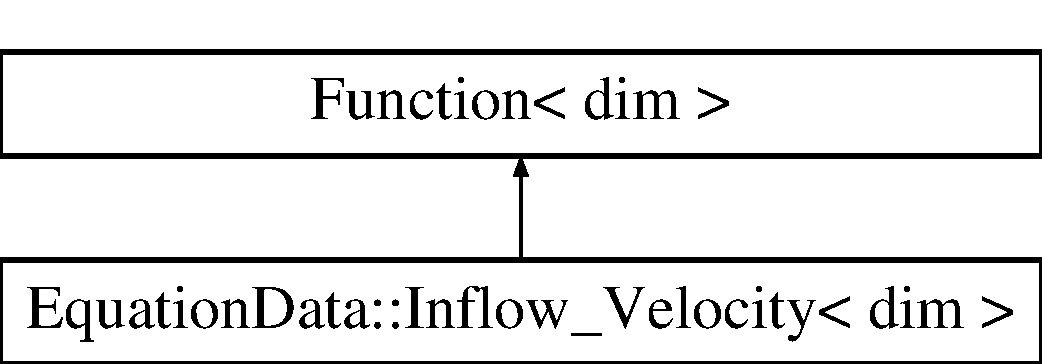
\includegraphics[height=2.000000cm]{class_equation_data_1_1_inflow___velocity}
\end{center}
\end{figure}
\subsubsection*{Public Member Functions}
\begin{DoxyCompactItemize}
\item 
\hyperlink{class_equation_data_1_1_inflow___velocity_ac5035db1e557027579fd3b3c0220c671}{Inflow\+\_\+\+Velocity} (double, unsigned int)
\item 
virtual double \hyperlink{class_equation_data_1_1_inflow___velocity_a986662426fb6b3685ced24ce676a6ac4}{value} (const Point$<$ dim $>$ \&p, const unsigned int component=0) const 
\item 
virtual void \hyperlink{class_equation_data_1_1_inflow___velocity_aad33ff25f7b8e2260cb40311d0b15aa6}{vector\+\_\+value} (const Point$<$ dim $>$ \&p, Vector$<$ double $>$ \&\hyperlink{class_equation_data_1_1_inflow___velocity_a986662426fb6b3685ced24ce676a6ac4}{value}) const 
\item 
virtual void \hyperlink{class_equation_data_1_1_inflow___velocity_a777730a2849272dfa7b3acb5cd83106f}{vector\+\_\+value\+\_\+list} (const std\+::vector$<$ Point$<$ dim $>$ $>$ \&p, std\+::vector$<$ Vector$<$ double $>$ $>$ \&values) const 
\end{DoxyCompactItemize}
\subsubsection*{Public Attributes}
\begin{DoxyCompactItemize}
\item 
double \hyperlink{class_equation_data_1_1_inflow___velocity_a00fdc2d87172dbf05e274529d53e4874}{init\+\_\+mean\+\_\+vel}
\item 
unsigned int \hyperlink{class_equation_data_1_1_inflow___velocity_affb59b1d9b0d574a0aec58652b6dff88}{which\+\_\+inflow\+\_\+type}
\end{DoxyCompactItemize}


\subsubsection{Constructor \& Destructor Documentation}
\hypertarget{class_equation_data_1_1_inflow___velocity_ac5035db1e557027579fd3b3c0220c671}{}\index{Equation\+Data\+::\+Inflow\+\_\+\+Velocity@{Equation\+Data\+::\+Inflow\+\_\+\+Velocity}!Inflow\+\_\+\+Velocity@{Inflow\+\_\+\+Velocity}}
\index{Inflow\+\_\+\+Velocity@{Inflow\+\_\+\+Velocity}!Equation\+Data\+::\+Inflow\+\_\+\+Velocity@{Equation\+Data\+::\+Inflow\+\_\+\+Velocity}}
\paragraph[{Inflow\+\_\+\+Velocity(double, unsigned int)}]{\setlength{\rightskip}{0pt plus 5cm}template$<$int dim$>$ {\bf Equation\+Data\+::\+Inflow\+\_\+\+Velocity}$<$ dim $>$\+::{\bf Inflow\+\_\+\+Velocity} (
\begin{DoxyParamCaption}
\item[{double}]{init\+\_\+mean\+\_\+vel, }
\item[{unsigned int}]{which\+\_\+inflow\+\_\+type}
\end{DoxyParamCaption}
)}\label{class_equation_data_1_1_inflow___velocity_ac5035db1e557027579fd3b3c0220c671}


\subsubsection{Member Function Documentation}
\hypertarget{class_equation_data_1_1_inflow___velocity_a986662426fb6b3685ced24ce676a6ac4}{}\index{Equation\+Data\+::\+Inflow\+\_\+\+Velocity@{Equation\+Data\+::\+Inflow\+\_\+\+Velocity}!value@{value}}
\index{value@{value}!Equation\+Data\+::\+Inflow\+\_\+\+Velocity@{Equation\+Data\+::\+Inflow\+\_\+\+Velocity}}
\paragraph[{value(const Point$<$ dim $>$ \&p, const unsigned int component=0) const }]{\setlength{\rightskip}{0pt plus 5cm}template$<$int dim$>$ double {\bf Equation\+Data\+::\+Inflow\+\_\+\+Velocity}$<$ dim $>$\+::value (
\begin{DoxyParamCaption}
\item[{const Point$<$ dim $>$ \&}]{p, }
\item[{const unsigned int}]{component = {\ttfamily 0}}
\end{DoxyParamCaption}
) const\hspace{0.3cm}{\ttfamily [virtual]}}\label{class_equation_data_1_1_inflow___velocity_a986662426fb6b3685ced24ce676a6ac4}
\hypertarget{class_equation_data_1_1_inflow___velocity_aad33ff25f7b8e2260cb40311d0b15aa6}{}\index{Equation\+Data\+::\+Inflow\+\_\+\+Velocity@{Equation\+Data\+::\+Inflow\+\_\+\+Velocity}!vector\+\_\+value@{vector\+\_\+value}}
\index{vector\+\_\+value@{vector\+\_\+value}!Equation\+Data\+::\+Inflow\+\_\+\+Velocity@{Equation\+Data\+::\+Inflow\+\_\+\+Velocity}}
\paragraph[{vector\+\_\+value(const Point$<$ dim $>$ \&p, Vector$<$ double $>$ \&value) const }]{\setlength{\rightskip}{0pt plus 5cm}template$<$int dim$>$ void {\bf Equation\+Data\+::\+Inflow\+\_\+\+Velocity}$<$ dim $>$\+::vector\+\_\+value (
\begin{DoxyParamCaption}
\item[{const Point$<$ dim $>$ \&}]{p, }
\item[{Vector$<$ double $>$ \&}]{value}
\end{DoxyParamCaption}
) const\hspace{0.3cm}{\ttfamily [virtual]}}\label{class_equation_data_1_1_inflow___velocity_aad33ff25f7b8e2260cb40311d0b15aa6}
\hypertarget{class_equation_data_1_1_inflow___velocity_a777730a2849272dfa7b3acb5cd83106f}{}\index{Equation\+Data\+::\+Inflow\+\_\+\+Velocity@{Equation\+Data\+::\+Inflow\+\_\+\+Velocity}!vector\+\_\+value\+\_\+list@{vector\+\_\+value\+\_\+list}}
\index{vector\+\_\+value\+\_\+list@{vector\+\_\+value\+\_\+list}!Equation\+Data\+::\+Inflow\+\_\+\+Velocity@{Equation\+Data\+::\+Inflow\+\_\+\+Velocity}}
\paragraph[{vector\+\_\+value\+\_\+list(const std\+::vector$<$ Point$<$ dim $>$ $>$ \&p, std\+::vector$<$ Vector$<$ double $>$ $>$ \&values) const }]{\setlength{\rightskip}{0pt plus 5cm}template$<$int dim$>$ void {\bf Equation\+Data\+::\+Inflow\+\_\+\+Velocity}$<$ dim $>$\+::vector\+\_\+value\+\_\+list (
\begin{DoxyParamCaption}
\item[{const std\+::vector$<$ Point$<$ dim $>$ $>$ \&}]{p, }
\item[{std\+::vector$<$ Vector$<$ double $>$ $>$ \&}]{values}
\end{DoxyParamCaption}
) const\hspace{0.3cm}{\ttfamily [virtual]}}\label{class_equation_data_1_1_inflow___velocity_a777730a2849272dfa7b3acb5cd83106f}


\subsubsection{Member Data Documentation}
\hypertarget{class_equation_data_1_1_inflow___velocity_a00fdc2d87172dbf05e274529d53e4874}{}\index{Equation\+Data\+::\+Inflow\+\_\+\+Velocity@{Equation\+Data\+::\+Inflow\+\_\+\+Velocity}!init\+\_\+mean\+\_\+vel@{init\+\_\+mean\+\_\+vel}}
\index{init\+\_\+mean\+\_\+vel@{init\+\_\+mean\+\_\+vel}!Equation\+Data\+::\+Inflow\+\_\+\+Velocity@{Equation\+Data\+::\+Inflow\+\_\+\+Velocity}}
\paragraph[{init\+\_\+mean\+\_\+vel}]{\setlength{\rightskip}{0pt plus 5cm}template$<$int dim$>$ double {\bf Equation\+Data\+::\+Inflow\+\_\+\+Velocity}$<$ dim $>$\+::init\+\_\+mean\+\_\+vel}\label{class_equation_data_1_1_inflow___velocity_a00fdc2d87172dbf05e274529d53e4874}
\hypertarget{class_equation_data_1_1_inflow___velocity_affb59b1d9b0d574a0aec58652b6dff88}{}\index{Equation\+Data\+::\+Inflow\+\_\+\+Velocity@{Equation\+Data\+::\+Inflow\+\_\+\+Velocity}!which\+\_\+inflow\+\_\+type@{which\+\_\+inflow\+\_\+type}}
\index{which\+\_\+inflow\+\_\+type@{which\+\_\+inflow\+\_\+type}!Equation\+Data\+::\+Inflow\+\_\+\+Velocity@{Equation\+Data\+::\+Inflow\+\_\+\+Velocity}}
\paragraph[{which\+\_\+inflow\+\_\+type}]{\setlength{\rightskip}{0pt plus 5cm}template$<$int dim$>$ unsigned int {\bf Equation\+Data\+::\+Inflow\+\_\+\+Velocity}$<$ dim $>$\+::which\+\_\+inflow\+\_\+type}\label{class_equation_data_1_1_inflow___velocity_affb59b1d9b0d574a0aec58652b6dff88}


The documentation for this class was generated from the following file\+:\begin{DoxyCompactItemize}
\item 
/\+Users/miranus/work/\+Devs/miscible\+\_\+mixing\+\_\+series/miscible\+\_\+mixing/include/mismix/\hyperlink{equation__data_8h}{equation\+\_\+data.\+h}\end{DoxyCompactItemize}

\hypertarget{class_equation_data_1_1_outflow___pressure}{}\section{Equation\+Data\+:\+:Outflow\+\_\+\+Pressure$<$ dim $>$ Class Template Reference}
\label{class_equation_data_1_1_outflow___pressure}\index{Equation\+Data\+::\+Outflow\+\_\+\+Pressure$<$ dim $>$@{Equation\+Data\+::\+Outflow\+\_\+\+Pressure$<$ dim $>$}}


{\ttfamily \#include $<$equation\+\_\+data.\+h$>$}

Inheritance diagram for Equation\+Data\+:\+:Outflow\+\_\+\+Pressure$<$ dim $>$\+:\begin{figure}[H]
\begin{center}
\leavevmode
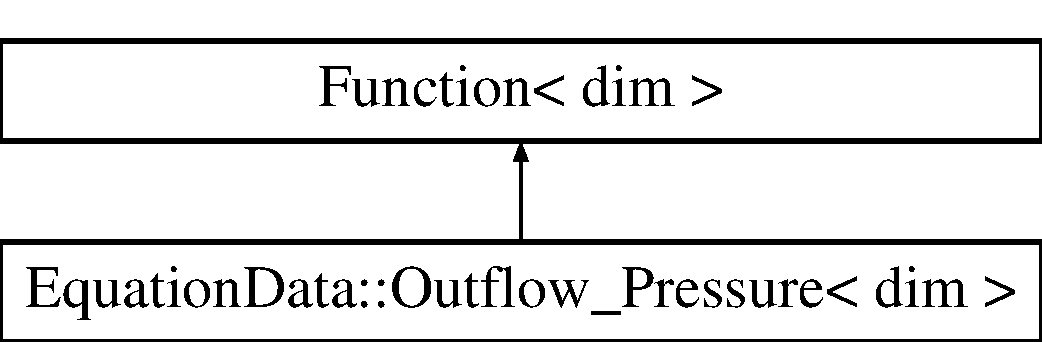
\includegraphics[height=2.000000cm]{class_equation_data_1_1_outflow___pressure}
\end{center}
\end{figure}
\subsection*{Public Member Functions}
\begin{DoxyCompactItemize}
\item 
\hyperlink{class_equation_data_1_1_outflow___pressure_a39cac043cd06378017efd9f9dfc2d40b}{Outflow\+\_\+\+Pressure} (double, double)
\item 
virtual double \hyperlink{class_equation_data_1_1_outflow___pressure_a48baf3b5f5a0b2ae4cdefeb62b429ca6}{value} (const Point$<$ dim $>$ \&p, const unsigned int component=0) const 
\item 
virtual void \hyperlink{class_equation_data_1_1_outflow___pressure_a430252223a17d71b8e10f76fb4bce313}{vector\+\_\+value} (const Point$<$ dim $>$ \&p, Vector$<$ double $>$ \&\hyperlink{class_equation_data_1_1_outflow___pressure_a48baf3b5f5a0b2ae4cdefeb62b429ca6}{value}) const 
\item 
virtual void \hyperlink{class_equation_data_1_1_outflow___pressure_a31c63da8138ec9837790878952008ba9}{vector\+\_\+value\+\_\+list} (const std\+::vector$<$ Point$<$ dim $>$ $>$ \&p, std\+::vector$<$ Vector$<$ double $>$ $>$ \&values) const 
\end{DoxyCompactItemize}
\subsection*{Public Attributes}
\begin{DoxyCompactItemize}
\item 
double \hyperlink{class_equation_data_1_1_outflow___pressure_ad4bf45eecee64a2045142e27fe8285ec}{inclined\+\_\+angle}
\item 
double \hyperlink{class_equation_data_1_1_outflow___pressure_acf53b90f3e6cc7f39883c415ff15c67e}{Froude\+\_\+number}
\end{DoxyCompactItemize}


\subsection{Constructor \& Destructor Documentation}
\hypertarget{class_equation_data_1_1_outflow___pressure_a39cac043cd06378017efd9f9dfc2d40b}{}\index{Equation\+Data\+::\+Outflow\+\_\+\+Pressure@{Equation\+Data\+::\+Outflow\+\_\+\+Pressure}!Outflow\+\_\+\+Pressure@{Outflow\+\_\+\+Pressure}}
\index{Outflow\+\_\+\+Pressure@{Outflow\+\_\+\+Pressure}!Equation\+Data\+::\+Outflow\+\_\+\+Pressure@{Equation\+Data\+::\+Outflow\+\_\+\+Pressure}}
\subsubsection[{Outflow\+\_\+\+Pressure(double, double)}]{\setlength{\rightskip}{0pt plus 5cm}template$<$int dim$>$ {\bf Equation\+Data\+::\+Outflow\+\_\+\+Pressure}$<$ dim $>$\+::{\bf Outflow\+\_\+\+Pressure} (
\begin{DoxyParamCaption}
\item[{double}]{inclined\+\_\+angle, }
\item[{double}]{Froude\+\_\+number}
\end{DoxyParamCaption}
)}\label{class_equation_data_1_1_outflow___pressure_a39cac043cd06378017efd9f9dfc2d40b}


\subsection{Member Function Documentation}
\hypertarget{class_equation_data_1_1_outflow___pressure_a48baf3b5f5a0b2ae4cdefeb62b429ca6}{}\index{Equation\+Data\+::\+Outflow\+\_\+\+Pressure@{Equation\+Data\+::\+Outflow\+\_\+\+Pressure}!value@{value}}
\index{value@{value}!Equation\+Data\+::\+Outflow\+\_\+\+Pressure@{Equation\+Data\+::\+Outflow\+\_\+\+Pressure}}
\subsubsection[{value(const Point$<$ dim $>$ \&p, const unsigned int component=0) const }]{\setlength{\rightskip}{0pt plus 5cm}template$<$int dim$>$ double {\bf Equation\+Data\+::\+Outflow\+\_\+\+Pressure}$<$ dim $>$\+::value (
\begin{DoxyParamCaption}
\item[{const Point$<$ dim $>$ \&}]{p, }
\item[{const unsigned int}]{component = {\ttfamily 0}}
\end{DoxyParamCaption}
) const\hspace{0.3cm}{\ttfamily [virtual]}}\label{class_equation_data_1_1_outflow___pressure_a48baf3b5f5a0b2ae4cdefeb62b429ca6}
\hypertarget{class_equation_data_1_1_outflow___pressure_a430252223a17d71b8e10f76fb4bce313}{}\index{Equation\+Data\+::\+Outflow\+\_\+\+Pressure@{Equation\+Data\+::\+Outflow\+\_\+\+Pressure}!vector\+\_\+value@{vector\+\_\+value}}
\index{vector\+\_\+value@{vector\+\_\+value}!Equation\+Data\+::\+Outflow\+\_\+\+Pressure@{Equation\+Data\+::\+Outflow\+\_\+\+Pressure}}
\subsubsection[{vector\+\_\+value(const Point$<$ dim $>$ \&p, Vector$<$ double $>$ \&value) const }]{\setlength{\rightskip}{0pt plus 5cm}template$<$int dim$>$ void {\bf Equation\+Data\+::\+Outflow\+\_\+\+Pressure}$<$ dim $>$\+::vector\+\_\+value (
\begin{DoxyParamCaption}
\item[{const Point$<$ dim $>$ \&}]{p, }
\item[{Vector$<$ double $>$ \&}]{value}
\end{DoxyParamCaption}
) const\hspace{0.3cm}{\ttfamily [virtual]}}\label{class_equation_data_1_1_outflow___pressure_a430252223a17d71b8e10f76fb4bce313}
\hypertarget{class_equation_data_1_1_outflow___pressure_a31c63da8138ec9837790878952008ba9}{}\index{Equation\+Data\+::\+Outflow\+\_\+\+Pressure@{Equation\+Data\+::\+Outflow\+\_\+\+Pressure}!vector\+\_\+value\+\_\+list@{vector\+\_\+value\+\_\+list}}
\index{vector\+\_\+value\+\_\+list@{vector\+\_\+value\+\_\+list}!Equation\+Data\+::\+Outflow\+\_\+\+Pressure@{Equation\+Data\+::\+Outflow\+\_\+\+Pressure}}
\subsubsection[{vector\+\_\+value\+\_\+list(const std\+::vector$<$ Point$<$ dim $>$ $>$ \&p, std\+::vector$<$ Vector$<$ double $>$ $>$ \&values) const }]{\setlength{\rightskip}{0pt plus 5cm}template$<$int dim$>$ void {\bf Equation\+Data\+::\+Outflow\+\_\+\+Pressure}$<$ dim $>$\+::vector\+\_\+value\+\_\+list (
\begin{DoxyParamCaption}
\item[{const std\+::vector$<$ Point$<$ dim $>$ $>$ \&}]{p, }
\item[{std\+::vector$<$ Vector$<$ double $>$ $>$ \&}]{values}
\end{DoxyParamCaption}
) const\hspace{0.3cm}{\ttfamily [virtual]}}\label{class_equation_data_1_1_outflow___pressure_a31c63da8138ec9837790878952008ba9}


\subsection{Member Data Documentation}
\hypertarget{class_equation_data_1_1_outflow___pressure_acf53b90f3e6cc7f39883c415ff15c67e}{}\index{Equation\+Data\+::\+Outflow\+\_\+\+Pressure@{Equation\+Data\+::\+Outflow\+\_\+\+Pressure}!Froude\+\_\+number@{Froude\+\_\+number}}
\index{Froude\+\_\+number@{Froude\+\_\+number}!Equation\+Data\+::\+Outflow\+\_\+\+Pressure@{Equation\+Data\+::\+Outflow\+\_\+\+Pressure}}
\subsubsection[{Froude\+\_\+number}]{\setlength{\rightskip}{0pt plus 5cm}template$<$int dim$>$ double {\bf Equation\+Data\+::\+Outflow\+\_\+\+Pressure}$<$ dim $>$\+::Froude\+\_\+number}\label{class_equation_data_1_1_outflow___pressure_acf53b90f3e6cc7f39883c415ff15c67e}
\hypertarget{class_equation_data_1_1_outflow___pressure_ad4bf45eecee64a2045142e27fe8285ec}{}\index{Equation\+Data\+::\+Outflow\+\_\+\+Pressure@{Equation\+Data\+::\+Outflow\+\_\+\+Pressure}!inclined\+\_\+angle@{inclined\+\_\+angle}}
\index{inclined\+\_\+angle@{inclined\+\_\+angle}!Equation\+Data\+::\+Outflow\+\_\+\+Pressure@{Equation\+Data\+::\+Outflow\+\_\+\+Pressure}}
\subsubsection[{inclined\+\_\+angle}]{\setlength{\rightskip}{0pt plus 5cm}template$<$int dim$>$ double {\bf Equation\+Data\+::\+Outflow\+\_\+\+Pressure}$<$ dim $>$\+::inclined\+\_\+angle}\label{class_equation_data_1_1_outflow___pressure_ad4bf45eecee64a2045142e27fe8285ec}


The documentation for this class was generated from the following file\+:\begin{DoxyCompactItemize}
\item 
/\+Users/miranus/work/\+Devs/miscible\+\_\+mixing\+\_\+series/miscible\+\_\+mixing/include/mismix/\hyperlink{equation__data_8h}{equation\+\_\+data.\+h}\end{DoxyCompactItemize}

\hypertarget{struct_u_b_c__mis__mixing_1_1_parameters}{}\section{U\+B\+C\+\_\+mis\+\_\+mixing$<$ dim $>$\+:\+:Parameters Struct Reference}
\label{struct_u_b_c__mis__mixing_1_1_parameters}\index{U\+B\+C\+\_\+mis\+\_\+mixing$<$ dim $>$\+::\+Parameters@{U\+B\+C\+\_\+mis\+\_\+mixing$<$ dim $>$\+::\+Parameters}}


{\ttfamily \#include $<$class.\+h$>$}

\subsection*{Public Member Functions}
\begin{DoxyCompactItemize}
\item 
\hyperlink{struct_u_b_c__mis__mixing_1_1_parameters_ad12e7c5f85bb4262a8713b9dbe250e32}{Parameters} (std\+::string \&parameters\+\_\+filename)
\item 
void \hyperlink{struct_u_b_c__mis__mixing_1_1_parameters_a09e79bcb48f2452c0228415b80fcd2a4}{parse\+\_\+parameters} (Parameter\+Handler \&prm)
\end{DoxyCompactItemize}
\subsection*{Static Public Member Functions}
\begin{DoxyCompactItemize}
\item 
static void \hyperlink{struct_u_b_c__mis__mixing_1_1_parameters_afe2e7d873f6f2670ae14f405aeaa67f1}{declare\+\_\+parameters} (Parameter\+Handler \&prm)
\end{DoxyCompactItemize}
\subsection*{Public Attributes}
\begin{DoxyCompactItemize}
\item 
std\+::string \hyperlink{struct_u_b_c__mis__mixing_1_1_parameters_aac252c8e13f3b044975af28070f2f756}{input\+\_\+mesh\+\_\+file}
\item 
Point$<$ dim $>$ \hyperlink{struct_u_b_c__mis__mixing_1_1_parameters_a24a6cf602ba017ad9f6504fb0ac083dd}{length\+\_\+of\+\_\+domain}
\item 
std\+::vector$<$ double $>$ \hyperlink{struct_u_b_c__mis__mixing_1_1_parameters_afb1287d7ff99313c1810618d9ba3e88d}{domain\+\_\+size}
\item 
std\+::vector$<$ double $>$ \hyperlink{struct_u_b_c__mis__mixing_1_1_parameters_ab5dd18f3f93bdac91f6d9ac765f7b0f2}{domain\+\_\+boundary}
\item 
unsigned int \hyperlink{struct_u_b_c__mis__mixing_1_1_parameters_a165c8e3abf1f41603587816b9016c612}{num\+\_\+element\+\_\+size}
\item 
unsigned int \hyperlink{struct_u_b_c__mis__mixing_1_1_parameters_a5a6ccb735b9c9aa71b1a9f85fc255315}{flow\+\_\+direction}
\item 
unsigned int \hyperlink{struct_u_b_c__mis__mixing_1_1_parameters_abaad9269bbf285086d40e5d8c3a6bbdd}{depth\+\_\+direction}
\item 
unsigned int \hyperlink{struct_u_b_c__mis__mixing_1_1_parameters_a1fb7274b6cc0e9ae893a3eab78c1e570}{latitude\+\_\+direction}
\item 
unsigned int \hyperlink{struct_u_b_c__mis__mixing_1_1_parameters_a3255a2145157e46b3d14e3eb39e4e518}{num\+\_\+slices\+\_\+domain}
\item 
bool \hyperlink{struct_u_b_c__mis__mixing_1_1_parameters_a4a1b3e4a709cf64c32d76435c2b090ac}{is\+\_\+symmetry\+\_\+boundary}
\item 
unsigned int \hyperlink{struct_u_b_c__mis__mixing_1_1_parameters_ae62b04744b770122b229fcabe1507274}{max\+\_\+grid\+\_\+level}
\item 
unsigned int \hyperlink{struct_u_b_c__mis__mixing_1_1_parameters_acace64be0270631ad440144d231187b0}{type\+\_\+adaptivity\+\_\+rule}
\item 
double \hyperlink{struct_u_b_c__mis__mixing_1_1_parameters_a13ee78e31e67b8d1f2cdc298e55fcad9}{error\+\_\+threshold}
\item 
double \hyperlink{struct_u_b_c__mis__mixing_1_1_parameters_a1cb12452f4e62d63463960a293b6fcfe}{ref\+\_\+crit}
\item 
double \hyperlink{struct_u_b_c__mis__mixing_1_1_parameters_aa269a4c7cf042c8ea3c2dd30d865a4dd}{coar\+\_\+crit}
\item 
unsigned int \hyperlink{struct_u_b_c__mis__mixing_1_1_parameters_a88702f3fc3a89e9e88bc06f8d5b2596f}{no\+\_\+refine\+\_\+period}
\item 
unsigned int \hyperlink{struct_u_b_c__mis__mixing_1_1_parameters_ac7af864aa24d111da0e46d45278950b0}{intial\+\_\+ratio\+\_\+refinement}
\item 
double \hyperlink{struct_u_b_c__mis__mixing_1_1_parameters_ad4e626698deb1d2d1e17d25ffade6433}{stabilization\+\_\+alpha}
\item 
double \hyperlink{struct_u_b_c__mis__mixing_1_1_parameters_aa88c59c293b2b4d7668c4ddaf48de937}{stabilization\+\_\+beta}
\item 
double \hyperlink{struct_u_b_c__mis__mixing_1_1_parameters_ab8699b436648320743f2d1601fa5fc1d}{stabilization\+\_\+c\+\_\+\+R}
\item 
unsigned int \hyperlink{struct_u_b_c__mis__mixing_1_1_parameters_ae719108e305df5ee2b950e8d058ccd89}{ist\+\_\+optimization\+\_\+method}
\item 
unsigned int \hyperlink{struct_u_b_c__mis__mixing_1_1_parameters_a621dda8ef2f8b914fc76b16da67d4869}{ist\+\_\+projection\+\_\+method}
\item 
unsigned int \hyperlink{struct_u_b_c__mis__mixing_1_1_parameters_ad7f05e11567b4ffcca1ab6d6d25e93cd}{ist\+\_\+pressure\+\_\+boundary}
\item 
unsigned int \hyperlink{struct_u_b_c__mis__mixing_1_1_parameters_a37b3342d98b8bc3b829a87981d2dc333}{ist\+\_\+flow\+\_\+source}
\item 
bool \hyperlink{struct_u_b_c__mis__mixing_1_1_parameters_a04908c7866d4e382771eef213f59ff4b}{ist\+\_\+uniform\+\_\+flow}
\item 
double \hyperlink{struct_u_b_c__mis__mixing_1_1_parameters_a856a4cd5f9549dda9bb66c0b8ac48a9e}{coeff\+\_\+relax\+\_\+div\+\_\+velocity}
\item 
unsigned int \hyperlink{struct_u_b_c__mis__mixing_1_1_parameters_aa1890b8ad18cc1099d1a5dca364908ae}{no\+\_\+steps\+\_\+for\+\_\+buffering}
\item 
double \hyperlink{struct_u_b_c__mis__mixing_1_1_parameters_a0211ea3e9c7db88805129ebd42cdceb9}{mesh\+\_\+speed}
\item 
unsigned int \hyperlink{struct_u_b_c__mis__mixing_1_1_parameters_ab32e4f6b79a7978b4439fa6407b44ea1}{dir\+\_\+concentration}
\item 
unsigned int \hyperlink{struct_u_b_c__mis__mixing_1_1_parameters_a81d4347712206d82a814748c69c2403a}{which\+\_\+method\+\_\+for\+\_\+c}
\item 
unsigned int \hyperlink{struct_u_b_c__mis__mixing_1_1_parameters_a01aafac2f16cff86d97c56971b556863}{which\+\_\+interpl\+\_\+c}
\item 
bool \hyperlink{struct_u_b_c__mis__mixing_1_1_parameters_a30c8c6eae5b3ba5970a52a4a2ca830ee}{ist\+\_\+add\+\_\+reinit}
\item 
double \hyperlink{struct_u_b_c__mis__mixing_1_1_parameters_a7fc00c11e3b0133cfd11fd066bf001b1}{coeff\+\_\+gamma\+\_\+grad\+\_\+div}
\item 
double \hyperlink{struct_u_b_c__mis__mixing_1_1_parameters_a349983dede465f524f0fe30f407cc1f9}{coeff\+\_\+arti\+\_\+viscosity}
\item 
double \hyperlink{struct_u_b_c__mis__mixing_1_1_parameters_aab1eefbfc10c6c2fbf6e17c0052e1e66}{maximum\+\_\+coeff\+\_\+arti\+\_\+viscosity}
\item 
bool \hyperlink{struct_u_b_c__mis__mixing_1_1_parameters_ae346c5f4dda04f8404da70094270f079}{exclude\+\_\+depth\+\_\+direction}
\item 
bool \hyperlink{struct_u_b_c__mis__mixing_1_1_parameters_ac75a0e2ec5561c641dbd46734330107a}{is\+\_\+verbal\+\_\+output}
\item 
double \hyperlink{struct_u_b_c__mis__mixing_1_1_parameters_ad34f1ebb7a819cabba044cae1af0b20d}{C\+F\+L\+\_\+number}
\item 
double \hyperlink{struct_u_b_c__mis__mixing_1_1_parameters_a943bbda36648d70b9538e331df84806e}{init\+\_\+sep\+\_\+x}
\item 
double \hyperlink{struct_u_b_c__mis__mixing_1_1_parameters_af85cef2fb611aff3bd93861f3dcedddd}{inclined\+\_\+angle}
\item 
double \hyperlink{struct_u_b_c__mis__mixing_1_1_parameters_a5d8b3abc5e87d4fb4e1f4df33f139670}{Atwood\+\_\+number}
\item 
double \hyperlink{struct_u_b_c__mis__mixing_1_1_parameters_a4e2da6f12751c597845f9ec3d3c124c2}{mean\+\_\+velocity\+\_\+inlet}
\item 
double \hyperlink{struct_u_b_c__mis__mixing_1_1_parameters_a82c51f961f3b029147cf4658e747096c}{inlet\+\_\+pressure}
\item 
double \hyperlink{struct_u_b_c__mis__mixing_1_1_parameters_a5247eabbe538c57069f6deefa55ac4d0}{viscosity\+\_\+ratio}
\item 
double \hyperlink{struct_u_b_c__mis__mixing_1_1_parameters_adc26ebcb3c943eaedd706e544895c178}{computed\+\_\+time\+\_\+step}
\item 
double \hyperlink{struct_u_b_c__mis__mixing_1_1_parameters_aee9ec05b6197d2bb35ac20df039700ff}{Reynolds\+\_\+number}
\item 
double \hyperlink{struct_u_b_c__mis__mixing_1_1_parameters_a83dc42fae26cde2af3c525e1eedc2f2a}{Froude\+\_\+number}
\item 
double \hyperlink{struct_u_b_c__mis__mixing_1_1_parameters_a8e98aacf8865ea49090c7e1ab2e460f5}{reference\+\_\+length}
\item 
double \hyperlink{struct_u_b_c__mis__mixing_1_1_parameters_abd08d52e96063537e6f97c7d3e50e830}{reference\+\_\+time}
\item 
double \hyperlink{struct_u_b_c__mis__mixing_1_1_parameters_a77b36610cc1cd6f5a07dc362c490d14d}{reference\+\_\+velocity}
\item 
bool \hyperlink{struct_u_b_c__mis__mixing_1_1_parameters_afbdbb5e1c2b5eab71b32ba865d33222c}{is\+\_\+density\+\_\+stable\+\_\+flow}
\item 
double \hyperlink{struct_u_b_c__mis__mixing_1_1_parameters_a70038d4135c91df2f4e5bc264436c537}{upstream\+\_\+concentr}
\item 
double \hyperlink{struct_u_b_c__mis__mixing_1_1_parameters_a398a5206459752d26d9851834bb8ef43}{downstream\+\_\+concentr}
\item 
double \hyperlink{struct_u_b_c__mis__mixing_1_1_parameters_acc367af009234bfb0e3c6af0d3872ce2}{mean\+\_\+viscosity}
\item 
double \hyperlink{struct_u_b_c__mis__mixing_1_1_parameters_a3fd3d1dc26004ad858cd04ed0fa80867}{ratio\+\_\+pow\+\_\+law}
\item 
double \hyperlink{struct_u_b_c__mis__mixing_1_1_parameters_a897cb7915129443818689eba5432f95e}{n\+\_\+pow\+\_\+law}
\item 
Point$<$ dim $>$ \hyperlink{struct_u_b_c__mis__mixing_1_1_parameters_a59c99018c9fa987dc19276029440d294}{inclined\+\_\+angle\+\_\+vector}
\item 
double \hyperlink{struct_u_b_c__mis__mixing_1_1_parameters_ab2db66b6fdb65bf7933aca4264f05a61}{tau\+\_\+step}
\item 
double \hyperlink{struct_u_b_c__mis__mixing_1_1_parameters_af91b302127463e747b8a814c51889eae}{eps\+\_\+v\+\_\+concentr}
\item 
unsigned int \hyperlink{struct_u_b_c__mis__mixing_1_1_parameters_a8df2e2964a815d173d465a9cdbb1fbc9}{degree\+\_\+of\+\_\+velocity}
\item 
unsigned int \hyperlink{struct_u_b_c__mis__mixing_1_1_parameters_aa64481fdb7859afd157860e5edb733fc}{degree\+\_\+of\+\_\+pressure}
\item 
unsigned int \hyperlink{struct_u_b_c__mis__mixing_1_1_parameters_a8f1bf5db819f09c9175a8bd7bf484971}{degree\+\_\+of\+\_\+concentr}
\item 
unsigned int \hyperlink{struct_u_b_c__mis__mixing_1_1_parameters_afefc28070f4288b949598723654baba4}{data\+\_\+id}
\item 
unsigned int \hyperlink{struct_u_b_c__mis__mixing_1_1_parameters_aa8503b9797f46dc16ba0fa2d7195a48f}{output\+\_\+fac\+\_\+vtu}
\item 
unsigned int \hyperlink{struct_u_b_c__mis__mixing_1_1_parameters_a5f77aeaec6daafeb048c81f8a422736d}{output\+\_\+fac\+\_\+data}
\item 
unsigned int \hyperlink{struct_u_b_c__mis__mixing_1_1_parameters_afd0d62eb8370ef34626e5ee3dac0e3a8}{number\+\_\+slices\+\_\+coarse\+\_\+mesh}
\item 
bool \hyperlink{struct_u_b_c__mis__mixing_1_1_parameters_a31244f6049cfffcb0f4bf5a80e2dcd5c}{is\+\_\+restart}
\item 
unsigned int \hyperlink{struct_u_b_c__mis__mixing_1_1_parameters_abdf2cfe7ef4efe3987f24f486cbbb368}{save\+\_\+fac\+\_\+period}
\item 
unsigned int \hyperlink{struct_u_b_c__mis__mixing_1_1_parameters_a59c23712227d6670b7e9d89e11a4ee04}{index\+\_\+for\+\_\+restart}
\item 
unsigned int \hyperlink{struct_u_b_c__mis__mixing_1_1_parameters_a1d34bd766f4ab94c96e72c8492f4f14e}{restart\+\_\+no\+\_\+timestep}
\item 
double \hyperlink{struct_u_b_c__mis__mixing_1_1_parameters_a489c02b628933ffd13120097d0f03f46}{check\+\_\+total\+\_\+time}
\item 
double \hyperlink{struct_u_b_c__mis__mixing_1_1_parameters_aaf644b08843115cd70c280ae7c00f252}{check\+\_\+total\+\_\+real\+\_\+time}
\item 
double \hyperlink{struct_u_b_c__mis__mixing_1_1_parameters_a233d28122449f3e894af1b5eb8cda925}{check\+\_\+current\+\_\+time\+\_\+step}
\item 
double \hyperlink{struct_u_b_c__mis__mixing_1_1_parameters_a073ad4dff68ff33bc25e01f21401958b}{check\+\_\+old\+\_\+time\+\_\+step}
\item 
double \hyperlink{struct_u_b_c__mis__mixing_1_1_parameters_a59539a74b2a7b5ada31dbb529ff21d9f}{eps\+\_\+ns}
\item 
double \hyperlink{struct_u_b_c__mis__mixing_1_1_parameters_a1d20b15ac5ae8fb61fab2027e003b010}{eps\+\_\+c}
\item 
unsigned int \hyperlink{struct_u_b_c__mis__mixing_1_1_parameters_adfd3cf708a892fea49d74dc2da238197}{kry\+\_\+size}
\item 
unsigned int \hyperlink{struct_u_b_c__mis__mixing_1_1_parameters_a958199fa5ce0d11d18572bbcc5dc3853}{no\+\_\+test\+\_\+case}
\end{DoxyCompactItemize}


\subsection{Constructor \& Destructor Documentation}
\hypertarget{struct_u_b_c__mis__mixing_1_1_parameters_ad12e7c5f85bb4262a8713b9dbe250e32}{}\index{U\+B\+C\+\_\+mis\+\_\+mixing\+::\+Parameters@{U\+B\+C\+\_\+mis\+\_\+mixing\+::\+Parameters}!Parameters@{Parameters}}
\index{Parameters@{Parameters}!U\+B\+C\+\_\+mis\+\_\+mixing\+::\+Parameters@{U\+B\+C\+\_\+mis\+\_\+mixing\+::\+Parameters}}
\subsubsection[{Parameters(std\+::string \&parameters\+\_\+filename)}]{\setlength{\rightskip}{0pt plus 5cm}template$<$int dim$>$ {\bf U\+B\+C\+\_\+mis\+\_\+mixing}$<$ dim $>$\+::Parameters\+::\+Parameters (
\begin{DoxyParamCaption}
\item[{std\+::string \&}]{parameters\+\_\+filename}
\end{DoxyParamCaption}
)}\label{struct_u_b_c__mis__mixing_1_1_parameters_ad12e7c5f85bb4262a8713b9dbe250e32}


\subsection{Member Function Documentation}
\hypertarget{struct_u_b_c__mis__mixing_1_1_parameters_afe2e7d873f6f2670ae14f405aeaa67f1}{}\index{U\+B\+C\+\_\+mis\+\_\+mixing\+::\+Parameters@{U\+B\+C\+\_\+mis\+\_\+mixing\+::\+Parameters}!declare\+\_\+parameters@{declare\+\_\+parameters}}
\index{declare\+\_\+parameters@{declare\+\_\+parameters}!U\+B\+C\+\_\+mis\+\_\+mixing\+::\+Parameters@{U\+B\+C\+\_\+mis\+\_\+mixing\+::\+Parameters}}
\subsubsection[{declare\+\_\+parameters(\+Parameter\+Handler \&prm)}]{\setlength{\rightskip}{0pt plus 5cm}template$<$int dim$>$ void {\bf U\+B\+C\+\_\+mis\+\_\+mixing}$<$ dim $>$\+::Parameters\+::declare\+\_\+parameters (
\begin{DoxyParamCaption}
\item[{Parameter\+Handler \&}]{prm}
\end{DoxyParamCaption}
)\hspace{0.3cm}{\ttfamily [static]}}\label{struct_u_b_c__mis__mixing_1_1_parameters_afe2e7d873f6f2670ae14f405aeaa67f1}
\hypertarget{struct_u_b_c__mis__mixing_1_1_parameters_a09e79bcb48f2452c0228415b80fcd2a4}{}\index{U\+B\+C\+\_\+mis\+\_\+mixing\+::\+Parameters@{U\+B\+C\+\_\+mis\+\_\+mixing\+::\+Parameters}!parse\+\_\+parameters@{parse\+\_\+parameters}}
\index{parse\+\_\+parameters@{parse\+\_\+parameters}!U\+B\+C\+\_\+mis\+\_\+mixing\+::\+Parameters@{U\+B\+C\+\_\+mis\+\_\+mixing\+::\+Parameters}}
\subsubsection[{parse\+\_\+parameters(\+Parameter\+Handler \&prm)}]{\setlength{\rightskip}{0pt plus 5cm}template$<$int dim$>$ void {\bf U\+B\+C\+\_\+mis\+\_\+mixing}$<$ dim $>$\+::Parameters\+::parse\+\_\+parameters (
\begin{DoxyParamCaption}
\item[{Parameter\+Handler \&}]{prm}
\end{DoxyParamCaption}
)}\label{struct_u_b_c__mis__mixing_1_1_parameters_a09e79bcb48f2452c0228415b80fcd2a4}


\subsection{Member Data Documentation}
\hypertarget{struct_u_b_c__mis__mixing_1_1_parameters_a5d8b3abc5e87d4fb4e1f4df33f139670}{}\index{U\+B\+C\+\_\+mis\+\_\+mixing\+::\+Parameters@{U\+B\+C\+\_\+mis\+\_\+mixing\+::\+Parameters}!Atwood\+\_\+number@{Atwood\+\_\+number}}
\index{Atwood\+\_\+number@{Atwood\+\_\+number}!U\+B\+C\+\_\+mis\+\_\+mixing\+::\+Parameters@{U\+B\+C\+\_\+mis\+\_\+mixing\+::\+Parameters}}
\subsubsection[{Atwood\+\_\+number}]{\setlength{\rightskip}{0pt plus 5cm}template$<$int dim$>$ double {\bf U\+B\+C\+\_\+mis\+\_\+mixing}$<$ dim $>$\+::Parameters\+::\+Atwood\+\_\+number}\label{struct_u_b_c__mis__mixing_1_1_parameters_a5d8b3abc5e87d4fb4e1f4df33f139670}
\hypertarget{struct_u_b_c__mis__mixing_1_1_parameters_ad34f1ebb7a819cabba044cae1af0b20d}{}\index{U\+B\+C\+\_\+mis\+\_\+mixing\+::\+Parameters@{U\+B\+C\+\_\+mis\+\_\+mixing\+::\+Parameters}!C\+F\+L\+\_\+number@{C\+F\+L\+\_\+number}}
\index{C\+F\+L\+\_\+number@{C\+F\+L\+\_\+number}!U\+B\+C\+\_\+mis\+\_\+mixing\+::\+Parameters@{U\+B\+C\+\_\+mis\+\_\+mixing\+::\+Parameters}}
\subsubsection[{C\+F\+L\+\_\+number}]{\setlength{\rightskip}{0pt plus 5cm}template$<$int dim$>$ double {\bf U\+B\+C\+\_\+mis\+\_\+mixing}$<$ dim $>$\+::Parameters\+::\+C\+F\+L\+\_\+number}\label{struct_u_b_c__mis__mixing_1_1_parameters_ad34f1ebb7a819cabba044cae1af0b20d}
\hypertarget{struct_u_b_c__mis__mixing_1_1_parameters_a233d28122449f3e894af1b5eb8cda925}{}\index{U\+B\+C\+\_\+mis\+\_\+mixing\+::\+Parameters@{U\+B\+C\+\_\+mis\+\_\+mixing\+::\+Parameters}!check\+\_\+current\+\_\+time\+\_\+step@{check\+\_\+current\+\_\+time\+\_\+step}}
\index{check\+\_\+current\+\_\+time\+\_\+step@{check\+\_\+current\+\_\+time\+\_\+step}!U\+B\+C\+\_\+mis\+\_\+mixing\+::\+Parameters@{U\+B\+C\+\_\+mis\+\_\+mixing\+::\+Parameters}}
\subsubsection[{check\+\_\+current\+\_\+time\+\_\+step}]{\setlength{\rightskip}{0pt plus 5cm}template$<$int dim$>$ double {\bf U\+B\+C\+\_\+mis\+\_\+mixing}$<$ dim $>$\+::Parameters\+::check\+\_\+current\+\_\+time\+\_\+step}\label{struct_u_b_c__mis__mixing_1_1_parameters_a233d28122449f3e894af1b5eb8cda925}
\hypertarget{struct_u_b_c__mis__mixing_1_1_parameters_a073ad4dff68ff33bc25e01f21401958b}{}\index{U\+B\+C\+\_\+mis\+\_\+mixing\+::\+Parameters@{U\+B\+C\+\_\+mis\+\_\+mixing\+::\+Parameters}!check\+\_\+old\+\_\+time\+\_\+step@{check\+\_\+old\+\_\+time\+\_\+step}}
\index{check\+\_\+old\+\_\+time\+\_\+step@{check\+\_\+old\+\_\+time\+\_\+step}!U\+B\+C\+\_\+mis\+\_\+mixing\+::\+Parameters@{U\+B\+C\+\_\+mis\+\_\+mixing\+::\+Parameters}}
\subsubsection[{check\+\_\+old\+\_\+time\+\_\+step}]{\setlength{\rightskip}{0pt plus 5cm}template$<$int dim$>$ double {\bf U\+B\+C\+\_\+mis\+\_\+mixing}$<$ dim $>$\+::Parameters\+::check\+\_\+old\+\_\+time\+\_\+step}\label{struct_u_b_c__mis__mixing_1_1_parameters_a073ad4dff68ff33bc25e01f21401958b}
\hypertarget{struct_u_b_c__mis__mixing_1_1_parameters_aaf644b08843115cd70c280ae7c00f252}{}\index{U\+B\+C\+\_\+mis\+\_\+mixing\+::\+Parameters@{U\+B\+C\+\_\+mis\+\_\+mixing\+::\+Parameters}!check\+\_\+total\+\_\+real\+\_\+time@{check\+\_\+total\+\_\+real\+\_\+time}}
\index{check\+\_\+total\+\_\+real\+\_\+time@{check\+\_\+total\+\_\+real\+\_\+time}!U\+B\+C\+\_\+mis\+\_\+mixing\+::\+Parameters@{U\+B\+C\+\_\+mis\+\_\+mixing\+::\+Parameters}}
\subsubsection[{check\+\_\+total\+\_\+real\+\_\+time}]{\setlength{\rightskip}{0pt plus 5cm}template$<$int dim$>$ double {\bf U\+B\+C\+\_\+mis\+\_\+mixing}$<$ dim $>$\+::Parameters\+::check\+\_\+total\+\_\+real\+\_\+time}\label{struct_u_b_c__mis__mixing_1_1_parameters_aaf644b08843115cd70c280ae7c00f252}
\hypertarget{struct_u_b_c__mis__mixing_1_1_parameters_a489c02b628933ffd13120097d0f03f46}{}\index{U\+B\+C\+\_\+mis\+\_\+mixing\+::\+Parameters@{U\+B\+C\+\_\+mis\+\_\+mixing\+::\+Parameters}!check\+\_\+total\+\_\+time@{check\+\_\+total\+\_\+time}}
\index{check\+\_\+total\+\_\+time@{check\+\_\+total\+\_\+time}!U\+B\+C\+\_\+mis\+\_\+mixing\+::\+Parameters@{U\+B\+C\+\_\+mis\+\_\+mixing\+::\+Parameters}}
\subsubsection[{check\+\_\+total\+\_\+time}]{\setlength{\rightskip}{0pt plus 5cm}template$<$int dim$>$ double {\bf U\+B\+C\+\_\+mis\+\_\+mixing}$<$ dim $>$\+::Parameters\+::check\+\_\+total\+\_\+time}\label{struct_u_b_c__mis__mixing_1_1_parameters_a489c02b628933ffd13120097d0f03f46}
\hypertarget{struct_u_b_c__mis__mixing_1_1_parameters_aa269a4c7cf042c8ea3c2dd30d865a4dd}{}\index{U\+B\+C\+\_\+mis\+\_\+mixing\+::\+Parameters@{U\+B\+C\+\_\+mis\+\_\+mixing\+::\+Parameters}!coar\+\_\+crit@{coar\+\_\+crit}}
\index{coar\+\_\+crit@{coar\+\_\+crit}!U\+B\+C\+\_\+mis\+\_\+mixing\+::\+Parameters@{U\+B\+C\+\_\+mis\+\_\+mixing\+::\+Parameters}}
\subsubsection[{coar\+\_\+crit}]{\setlength{\rightskip}{0pt plus 5cm}template$<$int dim$>$ double {\bf U\+B\+C\+\_\+mis\+\_\+mixing}$<$ dim $>$\+::Parameters\+::coar\+\_\+crit}\label{struct_u_b_c__mis__mixing_1_1_parameters_aa269a4c7cf042c8ea3c2dd30d865a4dd}
\hypertarget{struct_u_b_c__mis__mixing_1_1_parameters_a349983dede465f524f0fe30f407cc1f9}{}\index{U\+B\+C\+\_\+mis\+\_\+mixing\+::\+Parameters@{U\+B\+C\+\_\+mis\+\_\+mixing\+::\+Parameters}!coeff\+\_\+arti\+\_\+viscosity@{coeff\+\_\+arti\+\_\+viscosity}}
\index{coeff\+\_\+arti\+\_\+viscosity@{coeff\+\_\+arti\+\_\+viscosity}!U\+B\+C\+\_\+mis\+\_\+mixing\+::\+Parameters@{U\+B\+C\+\_\+mis\+\_\+mixing\+::\+Parameters}}
\subsubsection[{coeff\+\_\+arti\+\_\+viscosity}]{\setlength{\rightskip}{0pt plus 5cm}template$<$int dim$>$ double {\bf U\+B\+C\+\_\+mis\+\_\+mixing}$<$ dim $>$\+::Parameters\+::coeff\+\_\+arti\+\_\+viscosity}\label{struct_u_b_c__mis__mixing_1_1_parameters_a349983dede465f524f0fe30f407cc1f9}
\hypertarget{struct_u_b_c__mis__mixing_1_1_parameters_a7fc00c11e3b0133cfd11fd066bf001b1}{}\index{U\+B\+C\+\_\+mis\+\_\+mixing\+::\+Parameters@{U\+B\+C\+\_\+mis\+\_\+mixing\+::\+Parameters}!coeff\+\_\+gamma\+\_\+grad\+\_\+div@{coeff\+\_\+gamma\+\_\+grad\+\_\+div}}
\index{coeff\+\_\+gamma\+\_\+grad\+\_\+div@{coeff\+\_\+gamma\+\_\+grad\+\_\+div}!U\+B\+C\+\_\+mis\+\_\+mixing\+::\+Parameters@{U\+B\+C\+\_\+mis\+\_\+mixing\+::\+Parameters}}
\subsubsection[{coeff\+\_\+gamma\+\_\+grad\+\_\+div}]{\setlength{\rightskip}{0pt plus 5cm}template$<$int dim$>$ double {\bf U\+B\+C\+\_\+mis\+\_\+mixing}$<$ dim $>$\+::Parameters\+::coeff\+\_\+gamma\+\_\+grad\+\_\+div}\label{struct_u_b_c__mis__mixing_1_1_parameters_a7fc00c11e3b0133cfd11fd066bf001b1}
\hypertarget{struct_u_b_c__mis__mixing_1_1_parameters_a856a4cd5f9549dda9bb66c0b8ac48a9e}{}\index{U\+B\+C\+\_\+mis\+\_\+mixing\+::\+Parameters@{U\+B\+C\+\_\+mis\+\_\+mixing\+::\+Parameters}!coeff\+\_\+relax\+\_\+div\+\_\+velocity@{coeff\+\_\+relax\+\_\+div\+\_\+velocity}}
\index{coeff\+\_\+relax\+\_\+div\+\_\+velocity@{coeff\+\_\+relax\+\_\+div\+\_\+velocity}!U\+B\+C\+\_\+mis\+\_\+mixing\+::\+Parameters@{U\+B\+C\+\_\+mis\+\_\+mixing\+::\+Parameters}}
\subsubsection[{coeff\+\_\+relax\+\_\+div\+\_\+velocity}]{\setlength{\rightskip}{0pt plus 5cm}template$<$int dim$>$ double {\bf U\+B\+C\+\_\+mis\+\_\+mixing}$<$ dim $>$\+::Parameters\+::coeff\+\_\+relax\+\_\+div\+\_\+velocity}\label{struct_u_b_c__mis__mixing_1_1_parameters_a856a4cd5f9549dda9bb66c0b8ac48a9e}
\hypertarget{struct_u_b_c__mis__mixing_1_1_parameters_adc26ebcb3c943eaedd706e544895c178}{}\index{U\+B\+C\+\_\+mis\+\_\+mixing\+::\+Parameters@{U\+B\+C\+\_\+mis\+\_\+mixing\+::\+Parameters}!computed\+\_\+time\+\_\+step@{computed\+\_\+time\+\_\+step}}
\index{computed\+\_\+time\+\_\+step@{computed\+\_\+time\+\_\+step}!U\+B\+C\+\_\+mis\+\_\+mixing\+::\+Parameters@{U\+B\+C\+\_\+mis\+\_\+mixing\+::\+Parameters}}
\subsubsection[{computed\+\_\+time\+\_\+step}]{\setlength{\rightskip}{0pt plus 5cm}template$<$int dim$>$ double {\bf U\+B\+C\+\_\+mis\+\_\+mixing}$<$ dim $>$\+::Parameters\+::computed\+\_\+time\+\_\+step}\label{struct_u_b_c__mis__mixing_1_1_parameters_adc26ebcb3c943eaedd706e544895c178}
\hypertarget{struct_u_b_c__mis__mixing_1_1_parameters_afefc28070f4288b949598723654baba4}{}\index{U\+B\+C\+\_\+mis\+\_\+mixing\+::\+Parameters@{U\+B\+C\+\_\+mis\+\_\+mixing\+::\+Parameters}!data\+\_\+id@{data\+\_\+id}}
\index{data\+\_\+id@{data\+\_\+id}!U\+B\+C\+\_\+mis\+\_\+mixing\+::\+Parameters@{U\+B\+C\+\_\+mis\+\_\+mixing\+::\+Parameters}}
\subsubsection[{data\+\_\+id}]{\setlength{\rightskip}{0pt plus 5cm}template$<$int dim$>$ unsigned int {\bf U\+B\+C\+\_\+mis\+\_\+mixing}$<$ dim $>$\+::Parameters\+::data\+\_\+id}\label{struct_u_b_c__mis__mixing_1_1_parameters_afefc28070f4288b949598723654baba4}
\hypertarget{struct_u_b_c__mis__mixing_1_1_parameters_a8f1bf5db819f09c9175a8bd7bf484971}{}\index{U\+B\+C\+\_\+mis\+\_\+mixing\+::\+Parameters@{U\+B\+C\+\_\+mis\+\_\+mixing\+::\+Parameters}!degree\+\_\+of\+\_\+concentr@{degree\+\_\+of\+\_\+concentr}}
\index{degree\+\_\+of\+\_\+concentr@{degree\+\_\+of\+\_\+concentr}!U\+B\+C\+\_\+mis\+\_\+mixing\+::\+Parameters@{U\+B\+C\+\_\+mis\+\_\+mixing\+::\+Parameters}}
\subsubsection[{degree\+\_\+of\+\_\+concentr}]{\setlength{\rightskip}{0pt plus 5cm}template$<$int dim$>$ unsigned int {\bf U\+B\+C\+\_\+mis\+\_\+mixing}$<$ dim $>$\+::Parameters\+::degree\+\_\+of\+\_\+concentr}\label{struct_u_b_c__mis__mixing_1_1_parameters_a8f1bf5db819f09c9175a8bd7bf484971}
\hypertarget{struct_u_b_c__mis__mixing_1_1_parameters_aa64481fdb7859afd157860e5edb733fc}{}\index{U\+B\+C\+\_\+mis\+\_\+mixing\+::\+Parameters@{U\+B\+C\+\_\+mis\+\_\+mixing\+::\+Parameters}!degree\+\_\+of\+\_\+pressure@{degree\+\_\+of\+\_\+pressure}}
\index{degree\+\_\+of\+\_\+pressure@{degree\+\_\+of\+\_\+pressure}!U\+B\+C\+\_\+mis\+\_\+mixing\+::\+Parameters@{U\+B\+C\+\_\+mis\+\_\+mixing\+::\+Parameters}}
\subsubsection[{degree\+\_\+of\+\_\+pressure}]{\setlength{\rightskip}{0pt plus 5cm}template$<$int dim$>$ unsigned int {\bf U\+B\+C\+\_\+mis\+\_\+mixing}$<$ dim $>$\+::Parameters\+::degree\+\_\+of\+\_\+pressure}\label{struct_u_b_c__mis__mixing_1_1_parameters_aa64481fdb7859afd157860e5edb733fc}
\hypertarget{struct_u_b_c__mis__mixing_1_1_parameters_a8df2e2964a815d173d465a9cdbb1fbc9}{}\index{U\+B\+C\+\_\+mis\+\_\+mixing\+::\+Parameters@{U\+B\+C\+\_\+mis\+\_\+mixing\+::\+Parameters}!degree\+\_\+of\+\_\+velocity@{degree\+\_\+of\+\_\+velocity}}
\index{degree\+\_\+of\+\_\+velocity@{degree\+\_\+of\+\_\+velocity}!U\+B\+C\+\_\+mis\+\_\+mixing\+::\+Parameters@{U\+B\+C\+\_\+mis\+\_\+mixing\+::\+Parameters}}
\subsubsection[{degree\+\_\+of\+\_\+velocity}]{\setlength{\rightskip}{0pt plus 5cm}template$<$int dim$>$ unsigned int {\bf U\+B\+C\+\_\+mis\+\_\+mixing}$<$ dim $>$\+::Parameters\+::degree\+\_\+of\+\_\+velocity}\label{struct_u_b_c__mis__mixing_1_1_parameters_a8df2e2964a815d173d465a9cdbb1fbc9}
\hypertarget{struct_u_b_c__mis__mixing_1_1_parameters_abaad9269bbf285086d40e5d8c3a6bbdd}{}\index{U\+B\+C\+\_\+mis\+\_\+mixing\+::\+Parameters@{U\+B\+C\+\_\+mis\+\_\+mixing\+::\+Parameters}!depth\+\_\+direction@{depth\+\_\+direction}}
\index{depth\+\_\+direction@{depth\+\_\+direction}!U\+B\+C\+\_\+mis\+\_\+mixing\+::\+Parameters@{U\+B\+C\+\_\+mis\+\_\+mixing\+::\+Parameters}}
\subsubsection[{depth\+\_\+direction}]{\setlength{\rightskip}{0pt plus 5cm}template$<$int dim$>$ unsigned int {\bf U\+B\+C\+\_\+mis\+\_\+mixing}$<$ dim $>$\+::Parameters\+::depth\+\_\+direction}\label{struct_u_b_c__mis__mixing_1_1_parameters_abaad9269bbf285086d40e5d8c3a6bbdd}
\hypertarget{struct_u_b_c__mis__mixing_1_1_parameters_ab32e4f6b79a7978b4439fa6407b44ea1}{}\index{U\+B\+C\+\_\+mis\+\_\+mixing\+::\+Parameters@{U\+B\+C\+\_\+mis\+\_\+mixing\+::\+Parameters}!dir\+\_\+concentration@{dir\+\_\+concentration}}
\index{dir\+\_\+concentration@{dir\+\_\+concentration}!U\+B\+C\+\_\+mis\+\_\+mixing\+::\+Parameters@{U\+B\+C\+\_\+mis\+\_\+mixing\+::\+Parameters}}
\subsubsection[{dir\+\_\+concentration}]{\setlength{\rightskip}{0pt plus 5cm}template$<$int dim$>$ unsigned int {\bf U\+B\+C\+\_\+mis\+\_\+mixing}$<$ dim $>$\+::Parameters\+::dir\+\_\+concentration}\label{struct_u_b_c__mis__mixing_1_1_parameters_ab32e4f6b79a7978b4439fa6407b44ea1}
\hypertarget{struct_u_b_c__mis__mixing_1_1_parameters_ab5dd18f3f93bdac91f6d9ac765f7b0f2}{}\index{U\+B\+C\+\_\+mis\+\_\+mixing\+::\+Parameters@{U\+B\+C\+\_\+mis\+\_\+mixing\+::\+Parameters}!domain\+\_\+boundary@{domain\+\_\+boundary}}
\index{domain\+\_\+boundary@{domain\+\_\+boundary}!U\+B\+C\+\_\+mis\+\_\+mixing\+::\+Parameters@{U\+B\+C\+\_\+mis\+\_\+mixing\+::\+Parameters}}
\subsubsection[{domain\+\_\+boundary}]{\setlength{\rightskip}{0pt plus 5cm}template$<$int dim$>$ std\+::vector$<$double$>$ {\bf U\+B\+C\+\_\+mis\+\_\+mixing}$<$ dim $>$\+::Parameters\+::domain\+\_\+boundary}\label{struct_u_b_c__mis__mixing_1_1_parameters_ab5dd18f3f93bdac91f6d9ac765f7b0f2}
\hypertarget{struct_u_b_c__mis__mixing_1_1_parameters_afb1287d7ff99313c1810618d9ba3e88d}{}\index{U\+B\+C\+\_\+mis\+\_\+mixing\+::\+Parameters@{U\+B\+C\+\_\+mis\+\_\+mixing\+::\+Parameters}!domain\+\_\+size@{domain\+\_\+size}}
\index{domain\+\_\+size@{domain\+\_\+size}!U\+B\+C\+\_\+mis\+\_\+mixing\+::\+Parameters@{U\+B\+C\+\_\+mis\+\_\+mixing\+::\+Parameters}}
\subsubsection[{domain\+\_\+size}]{\setlength{\rightskip}{0pt plus 5cm}template$<$int dim$>$ std\+::vector$<$double$>$ {\bf U\+B\+C\+\_\+mis\+\_\+mixing}$<$ dim $>$\+::Parameters\+::domain\+\_\+size}\label{struct_u_b_c__mis__mixing_1_1_parameters_afb1287d7ff99313c1810618d9ba3e88d}
\hypertarget{struct_u_b_c__mis__mixing_1_1_parameters_a398a5206459752d26d9851834bb8ef43}{}\index{U\+B\+C\+\_\+mis\+\_\+mixing\+::\+Parameters@{U\+B\+C\+\_\+mis\+\_\+mixing\+::\+Parameters}!downstream\+\_\+concentr@{downstream\+\_\+concentr}}
\index{downstream\+\_\+concentr@{downstream\+\_\+concentr}!U\+B\+C\+\_\+mis\+\_\+mixing\+::\+Parameters@{U\+B\+C\+\_\+mis\+\_\+mixing\+::\+Parameters}}
\subsubsection[{downstream\+\_\+concentr}]{\setlength{\rightskip}{0pt plus 5cm}template$<$int dim$>$ double {\bf U\+B\+C\+\_\+mis\+\_\+mixing}$<$ dim $>$\+::Parameters\+::downstream\+\_\+concentr}\label{struct_u_b_c__mis__mixing_1_1_parameters_a398a5206459752d26d9851834bb8ef43}
\hypertarget{struct_u_b_c__mis__mixing_1_1_parameters_a1d20b15ac5ae8fb61fab2027e003b010}{}\index{U\+B\+C\+\_\+mis\+\_\+mixing\+::\+Parameters@{U\+B\+C\+\_\+mis\+\_\+mixing\+::\+Parameters}!eps\+\_\+c@{eps\+\_\+c}}
\index{eps\+\_\+c@{eps\+\_\+c}!U\+B\+C\+\_\+mis\+\_\+mixing\+::\+Parameters@{U\+B\+C\+\_\+mis\+\_\+mixing\+::\+Parameters}}
\subsubsection[{eps\+\_\+c}]{\setlength{\rightskip}{0pt plus 5cm}template$<$int dim$>$ double {\bf U\+B\+C\+\_\+mis\+\_\+mixing}$<$ dim $>$\+::Parameters\+::eps\+\_\+c}\label{struct_u_b_c__mis__mixing_1_1_parameters_a1d20b15ac5ae8fb61fab2027e003b010}
\hypertarget{struct_u_b_c__mis__mixing_1_1_parameters_a59539a74b2a7b5ada31dbb529ff21d9f}{}\index{U\+B\+C\+\_\+mis\+\_\+mixing\+::\+Parameters@{U\+B\+C\+\_\+mis\+\_\+mixing\+::\+Parameters}!eps\+\_\+ns@{eps\+\_\+ns}}
\index{eps\+\_\+ns@{eps\+\_\+ns}!U\+B\+C\+\_\+mis\+\_\+mixing\+::\+Parameters@{U\+B\+C\+\_\+mis\+\_\+mixing\+::\+Parameters}}
\subsubsection[{eps\+\_\+ns}]{\setlength{\rightskip}{0pt plus 5cm}template$<$int dim$>$ double {\bf U\+B\+C\+\_\+mis\+\_\+mixing}$<$ dim $>$\+::Parameters\+::eps\+\_\+ns}\label{struct_u_b_c__mis__mixing_1_1_parameters_a59539a74b2a7b5ada31dbb529ff21d9f}
\hypertarget{struct_u_b_c__mis__mixing_1_1_parameters_af91b302127463e747b8a814c51889eae}{}\index{U\+B\+C\+\_\+mis\+\_\+mixing\+::\+Parameters@{U\+B\+C\+\_\+mis\+\_\+mixing\+::\+Parameters}!eps\+\_\+v\+\_\+concentr@{eps\+\_\+v\+\_\+concentr}}
\index{eps\+\_\+v\+\_\+concentr@{eps\+\_\+v\+\_\+concentr}!U\+B\+C\+\_\+mis\+\_\+mixing\+::\+Parameters@{U\+B\+C\+\_\+mis\+\_\+mixing\+::\+Parameters}}
\subsubsection[{eps\+\_\+v\+\_\+concentr}]{\setlength{\rightskip}{0pt plus 5cm}template$<$int dim$>$ double {\bf U\+B\+C\+\_\+mis\+\_\+mixing}$<$ dim $>$\+::Parameters\+::eps\+\_\+v\+\_\+concentr}\label{struct_u_b_c__mis__mixing_1_1_parameters_af91b302127463e747b8a814c51889eae}
\hypertarget{struct_u_b_c__mis__mixing_1_1_parameters_a13ee78e31e67b8d1f2cdc298e55fcad9}{}\index{U\+B\+C\+\_\+mis\+\_\+mixing\+::\+Parameters@{U\+B\+C\+\_\+mis\+\_\+mixing\+::\+Parameters}!error\+\_\+threshold@{error\+\_\+threshold}}
\index{error\+\_\+threshold@{error\+\_\+threshold}!U\+B\+C\+\_\+mis\+\_\+mixing\+::\+Parameters@{U\+B\+C\+\_\+mis\+\_\+mixing\+::\+Parameters}}
\subsubsection[{error\+\_\+threshold}]{\setlength{\rightskip}{0pt plus 5cm}template$<$int dim$>$ double {\bf U\+B\+C\+\_\+mis\+\_\+mixing}$<$ dim $>$\+::Parameters\+::error\+\_\+threshold}\label{struct_u_b_c__mis__mixing_1_1_parameters_a13ee78e31e67b8d1f2cdc298e55fcad9}
\hypertarget{struct_u_b_c__mis__mixing_1_1_parameters_ae346c5f4dda04f8404da70094270f079}{}\index{U\+B\+C\+\_\+mis\+\_\+mixing\+::\+Parameters@{U\+B\+C\+\_\+mis\+\_\+mixing\+::\+Parameters}!exclude\+\_\+depth\+\_\+direction@{exclude\+\_\+depth\+\_\+direction}}
\index{exclude\+\_\+depth\+\_\+direction@{exclude\+\_\+depth\+\_\+direction}!U\+B\+C\+\_\+mis\+\_\+mixing\+::\+Parameters@{U\+B\+C\+\_\+mis\+\_\+mixing\+::\+Parameters}}
\subsubsection[{exclude\+\_\+depth\+\_\+direction}]{\setlength{\rightskip}{0pt plus 5cm}template$<$int dim$>$ bool {\bf U\+B\+C\+\_\+mis\+\_\+mixing}$<$ dim $>$\+::Parameters\+::exclude\+\_\+depth\+\_\+direction}\label{struct_u_b_c__mis__mixing_1_1_parameters_ae346c5f4dda04f8404da70094270f079}
\hypertarget{struct_u_b_c__mis__mixing_1_1_parameters_a5a6ccb735b9c9aa71b1a9f85fc255315}{}\index{U\+B\+C\+\_\+mis\+\_\+mixing\+::\+Parameters@{U\+B\+C\+\_\+mis\+\_\+mixing\+::\+Parameters}!flow\+\_\+direction@{flow\+\_\+direction}}
\index{flow\+\_\+direction@{flow\+\_\+direction}!U\+B\+C\+\_\+mis\+\_\+mixing\+::\+Parameters@{U\+B\+C\+\_\+mis\+\_\+mixing\+::\+Parameters}}
\subsubsection[{flow\+\_\+direction}]{\setlength{\rightskip}{0pt plus 5cm}template$<$int dim$>$ unsigned int {\bf U\+B\+C\+\_\+mis\+\_\+mixing}$<$ dim $>$\+::Parameters\+::flow\+\_\+direction}\label{struct_u_b_c__mis__mixing_1_1_parameters_a5a6ccb735b9c9aa71b1a9f85fc255315}
\hypertarget{struct_u_b_c__mis__mixing_1_1_parameters_a83dc42fae26cde2af3c525e1eedc2f2a}{}\index{U\+B\+C\+\_\+mis\+\_\+mixing\+::\+Parameters@{U\+B\+C\+\_\+mis\+\_\+mixing\+::\+Parameters}!Froude\+\_\+number@{Froude\+\_\+number}}
\index{Froude\+\_\+number@{Froude\+\_\+number}!U\+B\+C\+\_\+mis\+\_\+mixing\+::\+Parameters@{U\+B\+C\+\_\+mis\+\_\+mixing\+::\+Parameters}}
\subsubsection[{Froude\+\_\+number}]{\setlength{\rightskip}{0pt plus 5cm}template$<$int dim$>$ double {\bf U\+B\+C\+\_\+mis\+\_\+mixing}$<$ dim $>$\+::Parameters\+::\+Froude\+\_\+number}\label{struct_u_b_c__mis__mixing_1_1_parameters_a83dc42fae26cde2af3c525e1eedc2f2a}
\hypertarget{struct_u_b_c__mis__mixing_1_1_parameters_af85cef2fb611aff3bd93861f3dcedddd}{}\index{U\+B\+C\+\_\+mis\+\_\+mixing\+::\+Parameters@{U\+B\+C\+\_\+mis\+\_\+mixing\+::\+Parameters}!inclined\+\_\+angle@{inclined\+\_\+angle}}
\index{inclined\+\_\+angle@{inclined\+\_\+angle}!U\+B\+C\+\_\+mis\+\_\+mixing\+::\+Parameters@{U\+B\+C\+\_\+mis\+\_\+mixing\+::\+Parameters}}
\subsubsection[{inclined\+\_\+angle}]{\setlength{\rightskip}{0pt plus 5cm}template$<$int dim$>$ double {\bf U\+B\+C\+\_\+mis\+\_\+mixing}$<$ dim $>$\+::Parameters\+::inclined\+\_\+angle}\label{struct_u_b_c__mis__mixing_1_1_parameters_af85cef2fb611aff3bd93861f3dcedddd}
\hypertarget{struct_u_b_c__mis__mixing_1_1_parameters_a59c99018c9fa987dc19276029440d294}{}\index{U\+B\+C\+\_\+mis\+\_\+mixing\+::\+Parameters@{U\+B\+C\+\_\+mis\+\_\+mixing\+::\+Parameters}!inclined\+\_\+angle\+\_\+vector@{inclined\+\_\+angle\+\_\+vector}}
\index{inclined\+\_\+angle\+\_\+vector@{inclined\+\_\+angle\+\_\+vector}!U\+B\+C\+\_\+mis\+\_\+mixing\+::\+Parameters@{U\+B\+C\+\_\+mis\+\_\+mixing\+::\+Parameters}}
\subsubsection[{inclined\+\_\+angle\+\_\+vector}]{\setlength{\rightskip}{0pt plus 5cm}template$<$int dim$>$ Point$<$dim$>$ {\bf U\+B\+C\+\_\+mis\+\_\+mixing}$<$ dim $>$\+::Parameters\+::inclined\+\_\+angle\+\_\+vector}\label{struct_u_b_c__mis__mixing_1_1_parameters_a59c99018c9fa987dc19276029440d294}
\hypertarget{struct_u_b_c__mis__mixing_1_1_parameters_a59c23712227d6670b7e9d89e11a4ee04}{}\index{U\+B\+C\+\_\+mis\+\_\+mixing\+::\+Parameters@{U\+B\+C\+\_\+mis\+\_\+mixing\+::\+Parameters}!index\+\_\+for\+\_\+restart@{index\+\_\+for\+\_\+restart}}
\index{index\+\_\+for\+\_\+restart@{index\+\_\+for\+\_\+restart}!U\+B\+C\+\_\+mis\+\_\+mixing\+::\+Parameters@{U\+B\+C\+\_\+mis\+\_\+mixing\+::\+Parameters}}
\subsubsection[{index\+\_\+for\+\_\+restart}]{\setlength{\rightskip}{0pt plus 5cm}template$<$int dim$>$ unsigned int {\bf U\+B\+C\+\_\+mis\+\_\+mixing}$<$ dim $>$\+::Parameters\+::index\+\_\+for\+\_\+restart}\label{struct_u_b_c__mis__mixing_1_1_parameters_a59c23712227d6670b7e9d89e11a4ee04}
\hypertarget{struct_u_b_c__mis__mixing_1_1_parameters_a943bbda36648d70b9538e331df84806e}{}\index{U\+B\+C\+\_\+mis\+\_\+mixing\+::\+Parameters@{U\+B\+C\+\_\+mis\+\_\+mixing\+::\+Parameters}!init\+\_\+sep\+\_\+x@{init\+\_\+sep\+\_\+x}}
\index{init\+\_\+sep\+\_\+x@{init\+\_\+sep\+\_\+x}!U\+B\+C\+\_\+mis\+\_\+mixing\+::\+Parameters@{U\+B\+C\+\_\+mis\+\_\+mixing\+::\+Parameters}}
\subsubsection[{init\+\_\+sep\+\_\+x}]{\setlength{\rightskip}{0pt plus 5cm}template$<$int dim$>$ double {\bf U\+B\+C\+\_\+mis\+\_\+mixing}$<$ dim $>$\+::Parameters\+::init\+\_\+sep\+\_\+x}\label{struct_u_b_c__mis__mixing_1_1_parameters_a943bbda36648d70b9538e331df84806e}
\hypertarget{struct_u_b_c__mis__mixing_1_1_parameters_a82c51f961f3b029147cf4658e747096c}{}\index{U\+B\+C\+\_\+mis\+\_\+mixing\+::\+Parameters@{U\+B\+C\+\_\+mis\+\_\+mixing\+::\+Parameters}!inlet\+\_\+pressure@{inlet\+\_\+pressure}}
\index{inlet\+\_\+pressure@{inlet\+\_\+pressure}!U\+B\+C\+\_\+mis\+\_\+mixing\+::\+Parameters@{U\+B\+C\+\_\+mis\+\_\+mixing\+::\+Parameters}}
\subsubsection[{inlet\+\_\+pressure}]{\setlength{\rightskip}{0pt plus 5cm}template$<$int dim$>$ double {\bf U\+B\+C\+\_\+mis\+\_\+mixing}$<$ dim $>$\+::Parameters\+::inlet\+\_\+pressure}\label{struct_u_b_c__mis__mixing_1_1_parameters_a82c51f961f3b029147cf4658e747096c}
\hypertarget{struct_u_b_c__mis__mixing_1_1_parameters_aac252c8e13f3b044975af28070f2f756}{}\index{U\+B\+C\+\_\+mis\+\_\+mixing\+::\+Parameters@{U\+B\+C\+\_\+mis\+\_\+mixing\+::\+Parameters}!input\+\_\+mesh\+\_\+file@{input\+\_\+mesh\+\_\+file}}
\index{input\+\_\+mesh\+\_\+file@{input\+\_\+mesh\+\_\+file}!U\+B\+C\+\_\+mis\+\_\+mixing\+::\+Parameters@{U\+B\+C\+\_\+mis\+\_\+mixing\+::\+Parameters}}
\subsubsection[{input\+\_\+mesh\+\_\+file}]{\setlength{\rightskip}{0pt plus 5cm}template$<$int dim$>$ std\+::string {\bf U\+B\+C\+\_\+mis\+\_\+mixing}$<$ dim $>$\+::Parameters\+::input\+\_\+mesh\+\_\+file}\label{struct_u_b_c__mis__mixing_1_1_parameters_aac252c8e13f3b044975af28070f2f756}
\hypertarget{struct_u_b_c__mis__mixing_1_1_parameters_ac7af864aa24d111da0e46d45278950b0}{}\index{U\+B\+C\+\_\+mis\+\_\+mixing\+::\+Parameters@{U\+B\+C\+\_\+mis\+\_\+mixing\+::\+Parameters}!intial\+\_\+ratio\+\_\+refinement@{intial\+\_\+ratio\+\_\+refinement}}
\index{intial\+\_\+ratio\+\_\+refinement@{intial\+\_\+ratio\+\_\+refinement}!U\+B\+C\+\_\+mis\+\_\+mixing\+::\+Parameters@{U\+B\+C\+\_\+mis\+\_\+mixing\+::\+Parameters}}
\subsubsection[{intial\+\_\+ratio\+\_\+refinement}]{\setlength{\rightskip}{0pt plus 5cm}template$<$int dim$>$ unsigned int {\bf U\+B\+C\+\_\+mis\+\_\+mixing}$<$ dim $>$\+::Parameters\+::intial\+\_\+ratio\+\_\+refinement}\label{struct_u_b_c__mis__mixing_1_1_parameters_ac7af864aa24d111da0e46d45278950b0}
\hypertarget{struct_u_b_c__mis__mixing_1_1_parameters_afbdbb5e1c2b5eab71b32ba865d33222c}{}\index{U\+B\+C\+\_\+mis\+\_\+mixing\+::\+Parameters@{U\+B\+C\+\_\+mis\+\_\+mixing\+::\+Parameters}!is\+\_\+density\+\_\+stable\+\_\+flow@{is\+\_\+density\+\_\+stable\+\_\+flow}}
\index{is\+\_\+density\+\_\+stable\+\_\+flow@{is\+\_\+density\+\_\+stable\+\_\+flow}!U\+B\+C\+\_\+mis\+\_\+mixing\+::\+Parameters@{U\+B\+C\+\_\+mis\+\_\+mixing\+::\+Parameters}}
\subsubsection[{is\+\_\+density\+\_\+stable\+\_\+flow}]{\setlength{\rightskip}{0pt plus 5cm}template$<$int dim$>$ bool {\bf U\+B\+C\+\_\+mis\+\_\+mixing}$<$ dim $>$\+::Parameters\+::is\+\_\+density\+\_\+stable\+\_\+flow}\label{struct_u_b_c__mis__mixing_1_1_parameters_afbdbb5e1c2b5eab71b32ba865d33222c}
\hypertarget{struct_u_b_c__mis__mixing_1_1_parameters_a31244f6049cfffcb0f4bf5a80e2dcd5c}{}\index{U\+B\+C\+\_\+mis\+\_\+mixing\+::\+Parameters@{U\+B\+C\+\_\+mis\+\_\+mixing\+::\+Parameters}!is\+\_\+restart@{is\+\_\+restart}}
\index{is\+\_\+restart@{is\+\_\+restart}!U\+B\+C\+\_\+mis\+\_\+mixing\+::\+Parameters@{U\+B\+C\+\_\+mis\+\_\+mixing\+::\+Parameters}}
\subsubsection[{is\+\_\+restart}]{\setlength{\rightskip}{0pt plus 5cm}template$<$int dim$>$ bool {\bf U\+B\+C\+\_\+mis\+\_\+mixing}$<$ dim $>$\+::Parameters\+::is\+\_\+restart}\label{struct_u_b_c__mis__mixing_1_1_parameters_a31244f6049cfffcb0f4bf5a80e2dcd5c}
\hypertarget{struct_u_b_c__mis__mixing_1_1_parameters_a4a1b3e4a709cf64c32d76435c2b090ac}{}\index{U\+B\+C\+\_\+mis\+\_\+mixing\+::\+Parameters@{U\+B\+C\+\_\+mis\+\_\+mixing\+::\+Parameters}!is\+\_\+symmetry\+\_\+boundary@{is\+\_\+symmetry\+\_\+boundary}}
\index{is\+\_\+symmetry\+\_\+boundary@{is\+\_\+symmetry\+\_\+boundary}!U\+B\+C\+\_\+mis\+\_\+mixing\+::\+Parameters@{U\+B\+C\+\_\+mis\+\_\+mixing\+::\+Parameters}}
\subsubsection[{is\+\_\+symmetry\+\_\+boundary}]{\setlength{\rightskip}{0pt plus 5cm}template$<$int dim$>$ bool {\bf U\+B\+C\+\_\+mis\+\_\+mixing}$<$ dim $>$\+::Parameters\+::is\+\_\+symmetry\+\_\+boundary}\label{struct_u_b_c__mis__mixing_1_1_parameters_a4a1b3e4a709cf64c32d76435c2b090ac}
\hypertarget{struct_u_b_c__mis__mixing_1_1_parameters_ac75a0e2ec5561c641dbd46734330107a}{}\index{U\+B\+C\+\_\+mis\+\_\+mixing\+::\+Parameters@{U\+B\+C\+\_\+mis\+\_\+mixing\+::\+Parameters}!is\+\_\+verbal\+\_\+output@{is\+\_\+verbal\+\_\+output}}
\index{is\+\_\+verbal\+\_\+output@{is\+\_\+verbal\+\_\+output}!U\+B\+C\+\_\+mis\+\_\+mixing\+::\+Parameters@{U\+B\+C\+\_\+mis\+\_\+mixing\+::\+Parameters}}
\subsubsection[{is\+\_\+verbal\+\_\+output}]{\setlength{\rightskip}{0pt plus 5cm}template$<$int dim$>$ bool {\bf U\+B\+C\+\_\+mis\+\_\+mixing}$<$ dim $>$\+::Parameters\+::is\+\_\+verbal\+\_\+output}\label{struct_u_b_c__mis__mixing_1_1_parameters_ac75a0e2ec5561c641dbd46734330107a}
\hypertarget{struct_u_b_c__mis__mixing_1_1_parameters_a30c8c6eae5b3ba5970a52a4a2ca830ee}{}\index{U\+B\+C\+\_\+mis\+\_\+mixing\+::\+Parameters@{U\+B\+C\+\_\+mis\+\_\+mixing\+::\+Parameters}!ist\+\_\+add\+\_\+reinit@{ist\+\_\+add\+\_\+reinit}}
\index{ist\+\_\+add\+\_\+reinit@{ist\+\_\+add\+\_\+reinit}!U\+B\+C\+\_\+mis\+\_\+mixing\+::\+Parameters@{U\+B\+C\+\_\+mis\+\_\+mixing\+::\+Parameters}}
\subsubsection[{ist\+\_\+add\+\_\+reinit}]{\setlength{\rightskip}{0pt plus 5cm}template$<$int dim$>$ bool {\bf U\+B\+C\+\_\+mis\+\_\+mixing}$<$ dim $>$\+::Parameters\+::ist\+\_\+add\+\_\+reinit}\label{struct_u_b_c__mis__mixing_1_1_parameters_a30c8c6eae5b3ba5970a52a4a2ca830ee}
\hypertarget{struct_u_b_c__mis__mixing_1_1_parameters_a37b3342d98b8bc3b829a87981d2dc333}{}\index{U\+B\+C\+\_\+mis\+\_\+mixing\+::\+Parameters@{U\+B\+C\+\_\+mis\+\_\+mixing\+::\+Parameters}!ist\+\_\+flow\+\_\+source@{ist\+\_\+flow\+\_\+source}}
\index{ist\+\_\+flow\+\_\+source@{ist\+\_\+flow\+\_\+source}!U\+B\+C\+\_\+mis\+\_\+mixing\+::\+Parameters@{U\+B\+C\+\_\+mis\+\_\+mixing\+::\+Parameters}}
\subsubsection[{ist\+\_\+flow\+\_\+source}]{\setlength{\rightskip}{0pt plus 5cm}template$<$int dim$>$ unsigned int {\bf U\+B\+C\+\_\+mis\+\_\+mixing}$<$ dim $>$\+::Parameters\+::ist\+\_\+flow\+\_\+source}\label{struct_u_b_c__mis__mixing_1_1_parameters_a37b3342d98b8bc3b829a87981d2dc333}
\hypertarget{struct_u_b_c__mis__mixing_1_1_parameters_ae719108e305df5ee2b950e8d058ccd89}{}\index{U\+B\+C\+\_\+mis\+\_\+mixing\+::\+Parameters@{U\+B\+C\+\_\+mis\+\_\+mixing\+::\+Parameters}!ist\+\_\+optimization\+\_\+method@{ist\+\_\+optimization\+\_\+method}}
\index{ist\+\_\+optimization\+\_\+method@{ist\+\_\+optimization\+\_\+method}!U\+B\+C\+\_\+mis\+\_\+mixing\+::\+Parameters@{U\+B\+C\+\_\+mis\+\_\+mixing\+::\+Parameters}}
\subsubsection[{ist\+\_\+optimization\+\_\+method}]{\setlength{\rightskip}{0pt plus 5cm}template$<$int dim$>$ unsigned int {\bf U\+B\+C\+\_\+mis\+\_\+mixing}$<$ dim $>$\+::Parameters\+::ist\+\_\+optimization\+\_\+method}\label{struct_u_b_c__mis__mixing_1_1_parameters_ae719108e305df5ee2b950e8d058ccd89}
\hypertarget{struct_u_b_c__mis__mixing_1_1_parameters_ad7f05e11567b4ffcca1ab6d6d25e93cd}{}\index{U\+B\+C\+\_\+mis\+\_\+mixing\+::\+Parameters@{U\+B\+C\+\_\+mis\+\_\+mixing\+::\+Parameters}!ist\+\_\+pressure\+\_\+boundary@{ist\+\_\+pressure\+\_\+boundary}}
\index{ist\+\_\+pressure\+\_\+boundary@{ist\+\_\+pressure\+\_\+boundary}!U\+B\+C\+\_\+mis\+\_\+mixing\+::\+Parameters@{U\+B\+C\+\_\+mis\+\_\+mixing\+::\+Parameters}}
\subsubsection[{ist\+\_\+pressure\+\_\+boundary}]{\setlength{\rightskip}{0pt plus 5cm}template$<$int dim$>$ unsigned int {\bf U\+B\+C\+\_\+mis\+\_\+mixing}$<$ dim $>$\+::Parameters\+::ist\+\_\+pressure\+\_\+boundary}\label{struct_u_b_c__mis__mixing_1_1_parameters_ad7f05e11567b4ffcca1ab6d6d25e93cd}
\hypertarget{struct_u_b_c__mis__mixing_1_1_parameters_a621dda8ef2f8b914fc76b16da67d4869}{}\index{U\+B\+C\+\_\+mis\+\_\+mixing\+::\+Parameters@{U\+B\+C\+\_\+mis\+\_\+mixing\+::\+Parameters}!ist\+\_\+projection\+\_\+method@{ist\+\_\+projection\+\_\+method}}
\index{ist\+\_\+projection\+\_\+method@{ist\+\_\+projection\+\_\+method}!U\+B\+C\+\_\+mis\+\_\+mixing\+::\+Parameters@{U\+B\+C\+\_\+mis\+\_\+mixing\+::\+Parameters}}
\subsubsection[{ist\+\_\+projection\+\_\+method}]{\setlength{\rightskip}{0pt plus 5cm}template$<$int dim$>$ unsigned int {\bf U\+B\+C\+\_\+mis\+\_\+mixing}$<$ dim $>$\+::Parameters\+::ist\+\_\+projection\+\_\+method}\label{struct_u_b_c__mis__mixing_1_1_parameters_a621dda8ef2f8b914fc76b16da67d4869}
\hypertarget{struct_u_b_c__mis__mixing_1_1_parameters_a04908c7866d4e382771eef213f59ff4b}{}\index{U\+B\+C\+\_\+mis\+\_\+mixing\+::\+Parameters@{U\+B\+C\+\_\+mis\+\_\+mixing\+::\+Parameters}!ist\+\_\+uniform\+\_\+flow@{ist\+\_\+uniform\+\_\+flow}}
\index{ist\+\_\+uniform\+\_\+flow@{ist\+\_\+uniform\+\_\+flow}!U\+B\+C\+\_\+mis\+\_\+mixing\+::\+Parameters@{U\+B\+C\+\_\+mis\+\_\+mixing\+::\+Parameters}}
\subsubsection[{ist\+\_\+uniform\+\_\+flow}]{\setlength{\rightskip}{0pt plus 5cm}template$<$int dim$>$ bool {\bf U\+B\+C\+\_\+mis\+\_\+mixing}$<$ dim $>$\+::Parameters\+::ist\+\_\+uniform\+\_\+flow}\label{struct_u_b_c__mis__mixing_1_1_parameters_a04908c7866d4e382771eef213f59ff4b}
\hypertarget{struct_u_b_c__mis__mixing_1_1_parameters_adfd3cf708a892fea49d74dc2da238197}{}\index{U\+B\+C\+\_\+mis\+\_\+mixing\+::\+Parameters@{U\+B\+C\+\_\+mis\+\_\+mixing\+::\+Parameters}!kry\+\_\+size@{kry\+\_\+size}}
\index{kry\+\_\+size@{kry\+\_\+size}!U\+B\+C\+\_\+mis\+\_\+mixing\+::\+Parameters@{U\+B\+C\+\_\+mis\+\_\+mixing\+::\+Parameters}}
\subsubsection[{kry\+\_\+size}]{\setlength{\rightskip}{0pt plus 5cm}template$<$int dim$>$ unsigned int {\bf U\+B\+C\+\_\+mis\+\_\+mixing}$<$ dim $>$\+::Parameters\+::kry\+\_\+size}\label{struct_u_b_c__mis__mixing_1_1_parameters_adfd3cf708a892fea49d74dc2da238197}
\hypertarget{struct_u_b_c__mis__mixing_1_1_parameters_a1fb7274b6cc0e9ae893a3eab78c1e570}{}\index{U\+B\+C\+\_\+mis\+\_\+mixing\+::\+Parameters@{U\+B\+C\+\_\+mis\+\_\+mixing\+::\+Parameters}!latitude\+\_\+direction@{latitude\+\_\+direction}}
\index{latitude\+\_\+direction@{latitude\+\_\+direction}!U\+B\+C\+\_\+mis\+\_\+mixing\+::\+Parameters@{U\+B\+C\+\_\+mis\+\_\+mixing\+::\+Parameters}}
\subsubsection[{latitude\+\_\+direction}]{\setlength{\rightskip}{0pt plus 5cm}template$<$int dim$>$ unsigned int {\bf U\+B\+C\+\_\+mis\+\_\+mixing}$<$ dim $>$\+::Parameters\+::latitude\+\_\+direction}\label{struct_u_b_c__mis__mixing_1_1_parameters_a1fb7274b6cc0e9ae893a3eab78c1e570}
\hypertarget{struct_u_b_c__mis__mixing_1_1_parameters_a24a6cf602ba017ad9f6504fb0ac083dd}{}\index{U\+B\+C\+\_\+mis\+\_\+mixing\+::\+Parameters@{U\+B\+C\+\_\+mis\+\_\+mixing\+::\+Parameters}!length\+\_\+of\+\_\+domain@{length\+\_\+of\+\_\+domain}}
\index{length\+\_\+of\+\_\+domain@{length\+\_\+of\+\_\+domain}!U\+B\+C\+\_\+mis\+\_\+mixing\+::\+Parameters@{U\+B\+C\+\_\+mis\+\_\+mixing\+::\+Parameters}}
\subsubsection[{length\+\_\+of\+\_\+domain}]{\setlength{\rightskip}{0pt plus 5cm}template$<$int dim$>$ Point$<$dim$>$ {\bf U\+B\+C\+\_\+mis\+\_\+mixing}$<$ dim $>$\+::Parameters\+::length\+\_\+of\+\_\+domain}\label{struct_u_b_c__mis__mixing_1_1_parameters_a24a6cf602ba017ad9f6504fb0ac083dd}
\hypertarget{struct_u_b_c__mis__mixing_1_1_parameters_ae62b04744b770122b229fcabe1507274}{}\index{U\+B\+C\+\_\+mis\+\_\+mixing\+::\+Parameters@{U\+B\+C\+\_\+mis\+\_\+mixing\+::\+Parameters}!max\+\_\+grid\+\_\+level@{max\+\_\+grid\+\_\+level}}
\index{max\+\_\+grid\+\_\+level@{max\+\_\+grid\+\_\+level}!U\+B\+C\+\_\+mis\+\_\+mixing\+::\+Parameters@{U\+B\+C\+\_\+mis\+\_\+mixing\+::\+Parameters}}
\subsubsection[{max\+\_\+grid\+\_\+level}]{\setlength{\rightskip}{0pt plus 5cm}template$<$int dim$>$ unsigned int {\bf U\+B\+C\+\_\+mis\+\_\+mixing}$<$ dim $>$\+::Parameters\+::max\+\_\+grid\+\_\+level}\label{struct_u_b_c__mis__mixing_1_1_parameters_ae62b04744b770122b229fcabe1507274}
\hypertarget{struct_u_b_c__mis__mixing_1_1_parameters_aab1eefbfc10c6c2fbf6e17c0052e1e66}{}\index{U\+B\+C\+\_\+mis\+\_\+mixing\+::\+Parameters@{U\+B\+C\+\_\+mis\+\_\+mixing\+::\+Parameters}!maximum\+\_\+coeff\+\_\+arti\+\_\+viscosity@{maximum\+\_\+coeff\+\_\+arti\+\_\+viscosity}}
\index{maximum\+\_\+coeff\+\_\+arti\+\_\+viscosity@{maximum\+\_\+coeff\+\_\+arti\+\_\+viscosity}!U\+B\+C\+\_\+mis\+\_\+mixing\+::\+Parameters@{U\+B\+C\+\_\+mis\+\_\+mixing\+::\+Parameters}}
\subsubsection[{maximum\+\_\+coeff\+\_\+arti\+\_\+viscosity}]{\setlength{\rightskip}{0pt plus 5cm}template$<$int dim$>$ double {\bf U\+B\+C\+\_\+mis\+\_\+mixing}$<$ dim $>$\+::Parameters\+::maximum\+\_\+coeff\+\_\+arti\+\_\+viscosity}\label{struct_u_b_c__mis__mixing_1_1_parameters_aab1eefbfc10c6c2fbf6e17c0052e1e66}
\hypertarget{struct_u_b_c__mis__mixing_1_1_parameters_a4e2da6f12751c597845f9ec3d3c124c2}{}\index{U\+B\+C\+\_\+mis\+\_\+mixing\+::\+Parameters@{U\+B\+C\+\_\+mis\+\_\+mixing\+::\+Parameters}!mean\+\_\+velocity\+\_\+inlet@{mean\+\_\+velocity\+\_\+inlet}}
\index{mean\+\_\+velocity\+\_\+inlet@{mean\+\_\+velocity\+\_\+inlet}!U\+B\+C\+\_\+mis\+\_\+mixing\+::\+Parameters@{U\+B\+C\+\_\+mis\+\_\+mixing\+::\+Parameters}}
\subsubsection[{mean\+\_\+velocity\+\_\+inlet}]{\setlength{\rightskip}{0pt plus 5cm}template$<$int dim$>$ double {\bf U\+B\+C\+\_\+mis\+\_\+mixing}$<$ dim $>$\+::Parameters\+::mean\+\_\+velocity\+\_\+inlet}\label{struct_u_b_c__mis__mixing_1_1_parameters_a4e2da6f12751c597845f9ec3d3c124c2}
\hypertarget{struct_u_b_c__mis__mixing_1_1_parameters_acc367af009234bfb0e3c6af0d3872ce2}{}\index{U\+B\+C\+\_\+mis\+\_\+mixing\+::\+Parameters@{U\+B\+C\+\_\+mis\+\_\+mixing\+::\+Parameters}!mean\+\_\+viscosity@{mean\+\_\+viscosity}}
\index{mean\+\_\+viscosity@{mean\+\_\+viscosity}!U\+B\+C\+\_\+mis\+\_\+mixing\+::\+Parameters@{U\+B\+C\+\_\+mis\+\_\+mixing\+::\+Parameters}}
\subsubsection[{mean\+\_\+viscosity}]{\setlength{\rightskip}{0pt plus 5cm}template$<$int dim$>$ double {\bf U\+B\+C\+\_\+mis\+\_\+mixing}$<$ dim $>$\+::Parameters\+::mean\+\_\+viscosity}\label{struct_u_b_c__mis__mixing_1_1_parameters_acc367af009234bfb0e3c6af0d3872ce2}
\hypertarget{struct_u_b_c__mis__mixing_1_1_parameters_a0211ea3e9c7db88805129ebd42cdceb9}{}\index{U\+B\+C\+\_\+mis\+\_\+mixing\+::\+Parameters@{U\+B\+C\+\_\+mis\+\_\+mixing\+::\+Parameters}!mesh\+\_\+speed@{mesh\+\_\+speed}}
\index{mesh\+\_\+speed@{mesh\+\_\+speed}!U\+B\+C\+\_\+mis\+\_\+mixing\+::\+Parameters@{U\+B\+C\+\_\+mis\+\_\+mixing\+::\+Parameters}}
\subsubsection[{mesh\+\_\+speed}]{\setlength{\rightskip}{0pt plus 5cm}template$<$int dim$>$ double {\bf U\+B\+C\+\_\+mis\+\_\+mixing}$<$ dim $>$\+::Parameters\+::mesh\+\_\+speed}\label{struct_u_b_c__mis__mixing_1_1_parameters_a0211ea3e9c7db88805129ebd42cdceb9}
\hypertarget{struct_u_b_c__mis__mixing_1_1_parameters_a897cb7915129443818689eba5432f95e}{}\index{U\+B\+C\+\_\+mis\+\_\+mixing\+::\+Parameters@{U\+B\+C\+\_\+mis\+\_\+mixing\+::\+Parameters}!n\+\_\+pow\+\_\+law@{n\+\_\+pow\+\_\+law}}
\index{n\+\_\+pow\+\_\+law@{n\+\_\+pow\+\_\+law}!U\+B\+C\+\_\+mis\+\_\+mixing\+::\+Parameters@{U\+B\+C\+\_\+mis\+\_\+mixing\+::\+Parameters}}
\subsubsection[{n\+\_\+pow\+\_\+law}]{\setlength{\rightskip}{0pt plus 5cm}template$<$int dim$>$ double {\bf U\+B\+C\+\_\+mis\+\_\+mixing}$<$ dim $>$\+::Parameters\+::n\+\_\+pow\+\_\+law}\label{struct_u_b_c__mis__mixing_1_1_parameters_a897cb7915129443818689eba5432f95e}
\hypertarget{struct_u_b_c__mis__mixing_1_1_parameters_a88702f3fc3a89e9e88bc06f8d5b2596f}{}\index{U\+B\+C\+\_\+mis\+\_\+mixing\+::\+Parameters@{U\+B\+C\+\_\+mis\+\_\+mixing\+::\+Parameters}!no\+\_\+refine\+\_\+period@{no\+\_\+refine\+\_\+period}}
\index{no\+\_\+refine\+\_\+period@{no\+\_\+refine\+\_\+period}!U\+B\+C\+\_\+mis\+\_\+mixing\+::\+Parameters@{U\+B\+C\+\_\+mis\+\_\+mixing\+::\+Parameters}}
\subsubsection[{no\+\_\+refine\+\_\+period}]{\setlength{\rightskip}{0pt plus 5cm}template$<$int dim$>$ unsigned int {\bf U\+B\+C\+\_\+mis\+\_\+mixing}$<$ dim $>$\+::Parameters\+::no\+\_\+refine\+\_\+period}\label{struct_u_b_c__mis__mixing_1_1_parameters_a88702f3fc3a89e9e88bc06f8d5b2596f}
\hypertarget{struct_u_b_c__mis__mixing_1_1_parameters_aa1890b8ad18cc1099d1a5dca364908ae}{}\index{U\+B\+C\+\_\+mis\+\_\+mixing\+::\+Parameters@{U\+B\+C\+\_\+mis\+\_\+mixing\+::\+Parameters}!no\+\_\+steps\+\_\+for\+\_\+buffering@{no\+\_\+steps\+\_\+for\+\_\+buffering}}
\index{no\+\_\+steps\+\_\+for\+\_\+buffering@{no\+\_\+steps\+\_\+for\+\_\+buffering}!U\+B\+C\+\_\+mis\+\_\+mixing\+::\+Parameters@{U\+B\+C\+\_\+mis\+\_\+mixing\+::\+Parameters}}
\subsubsection[{no\+\_\+steps\+\_\+for\+\_\+buffering}]{\setlength{\rightskip}{0pt plus 5cm}template$<$int dim$>$ unsigned int {\bf U\+B\+C\+\_\+mis\+\_\+mixing}$<$ dim $>$\+::Parameters\+::no\+\_\+steps\+\_\+for\+\_\+buffering}\label{struct_u_b_c__mis__mixing_1_1_parameters_aa1890b8ad18cc1099d1a5dca364908ae}
\hypertarget{struct_u_b_c__mis__mixing_1_1_parameters_a958199fa5ce0d11d18572bbcc5dc3853}{}\index{U\+B\+C\+\_\+mis\+\_\+mixing\+::\+Parameters@{U\+B\+C\+\_\+mis\+\_\+mixing\+::\+Parameters}!no\+\_\+test\+\_\+case@{no\+\_\+test\+\_\+case}}
\index{no\+\_\+test\+\_\+case@{no\+\_\+test\+\_\+case}!U\+B\+C\+\_\+mis\+\_\+mixing\+::\+Parameters@{U\+B\+C\+\_\+mis\+\_\+mixing\+::\+Parameters}}
\subsubsection[{no\+\_\+test\+\_\+case}]{\setlength{\rightskip}{0pt plus 5cm}template$<$int dim$>$ unsigned int {\bf U\+B\+C\+\_\+mis\+\_\+mixing}$<$ dim $>$\+::Parameters\+::no\+\_\+test\+\_\+case}\label{struct_u_b_c__mis__mixing_1_1_parameters_a958199fa5ce0d11d18572bbcc5dc3853}
\hypertarget{struct_u_b_c__mis__mixing_1_1_parameters_a165c8e3abf1f41603587816b9016c612}{}\index{U\+B\+C\+\_\+mis\+\_\+mixing\+::\+Parameters@{U\+B\+C\+\_\+mis\+\_\+mixing\+::\+Parameters}!num\+\_\+element\+\_\+size@{num\+\_\+element\+\_\+size}}
\index{num\+\_\+element\+\_\+size@{num\+\_\+element\+\_\+size}!U\+B\+C\+\_\+mis\+\_\+mixing\+::\+Parameters@{U\+B\+C\+\_\+mis\+\_\+mixing\+::\+Parameters}}
\subsubsection[{num\+\_\+element\+\_\+size}]{\setlength{\rightskip}{0pt plus 5cm}template$<$int dim$>$ unsigned int {\bf U\+B\+C\+\_\+mis\+\_\+mixing}$<$ dim $>$\+::Parameters\+::num\+\_\+element\+\_\+size}\label{struct_u_b_c__mis__mixing_1_1_parameters_a165c8e3abf1f41603587816b9016c612}
\hypertarget{struct_u_b_c__mis__mixing_1_1_parameters_a3255a2145157e46b3d14e3eb39e4e518}{}\index{U\+B\+C\+\_\+mis\+\_\+mixing\+::\+Parameters@{U\+B\+C\+\_\+mis\+\_\+mixing\+::\+Parameters}!num\+\_\+slices\+\_\+domain@{num\+\_\+slices\+\_\+domain}}
\index{num\+\_\+slices\+\_\+domain@{num\+\_\+slices\+\_\+domain}!U\+B\+C\+\_\+mis\+\_\+mixing\+::\+Parameters@{U\+B\+C\+\_\+mis\+\_\+mixing\+::\+Parameters}}
\subsubsection[{num\+\_\+slices\+\_\+domain}]{\setlength{\rightskip}{0pt plus 5cm}template$<$int dim$>$ unsigned int {\bf U\+B\+C\+\_\+mis\+\_\+mixing}$<$ dim $>$\+::Parameters\+::num\+\_\+slices\+\_\+domain}\label{struct_u_b_c__mis__mixing_1_1_parameters_a3255a2145157e46b3d14e3eb39e4e518}
\hypertarget{struct_u_b_c__mis__mixing_1_1_parameters_afd0d62eb8370ef34626e5ee3dac0e3a8}{}\index{U\+B\+C\+\_\+mis\+\_\+mixing\+::\+Parameters@{U\+B\+C\+\_\+mis\+\_\+mixing\+::\+Parameters}!number\+\_\+slices\+\_\+coarse\+\_\+mesh@{number\+\_\+slices\+\_\+coarse\+\_\+mesh}}
\index{number\+\_\+slices\+\_\+coarse\+\_\+mesh@{number\+\_\+slices\+\_\+coarse\+\_\+mesh}!U\+B\+C\+\_\+mis\+\_\+mixing\+::\+Parameters@{U\+B\+C\+\_\+mis\+\_\+mixing\+::\+Parameters}}
\subsubsection[{number\+\_\+slices\+\_\+coarse\+\_\+mesh}]{\setlength{\rightskip}{0pt plus 5cm}template$<$int dim$>$ unsigned int {\bf U\+B\+C\+\_\+mis\+\_\+mixing}$<$ dim $>$\+::Parameters\+::number\+\_\+slices\+\_\+coarse\+\_\+mesh}\label{struct_u_b_c__mis__mixing_1_1_parameters_afd0d62eb8370ef34626e5ee3dac0e3a8}
\hypertarget{struct_u_b_c__mis__mixing_1_1_parameters_a5f77aeaec6daafeb048c81f8a422736d}{}\index{U\+B\+C\+\_\+mis\+\_\+mixing\+::\+Parameters@{U\+B\+C\+\_\+mis\+\_\+mixing\+::\+Parameters}!output\+\_\+fac\+\_\+data@{output\+\_\+fac\+\_\+data}}
\index{output\+\_\+fac\+\_\+data@{output\+\_\+fac\+\_\+data}!U\+B\+C\+\_\+mis\+\_\+mixing\+::\+Parameters@{U\+B\+C\+\_\+mis\+\_\+mixing\+::\+Parameters}}
\subsubsection[{output\+\_\+fac\+\_\+data}]{\setlength{\rightskip}{0pt plus 5cm}template$<$int dim$>$ unsigned int {\bf U\+B\+C\+\_\+mis\+\_\+mixing}$<$ dim $>$\+::Parameters\+::output\+\_\+fac\+\_\+data}\label{struct_u_b_c__mis__mixing_1_1_parameters_a5f77aeaec6daafeb048c81f8a422736d}
\hypertarget{struct_u_b_c__mis__mixing_1_1_parameters_aa8503b9797f46dc16ba0fa2d7195a48f}{}\index{U\+B\+C\+\_\+mis\+\_\+mixing\+::\+Parameters@{U\+B\+C\+\_\+mis\+\_\+mixing\+::\+Parameters}!output\+\_\+fac\+\_\+vtu@{output\+\_\+fac\+\_\+vtu}}
\index{output\+\_\+fac\+\_\+vtu@{output\+\_\+fac\+\_\+vtu}!U\+B\+C\+\_\+mis\+\_\+mixing\+::\+Parameters@{U\+B\+C\+\_\+mis\+\_\+mixing\+::\+Parameters}}
\subsubsection[{output\+\_\+fac\+\_\+vtu}]{\setlength{\rightskip}{0pt plus 5cm}template$<$int dim$>$ unsigned int {\bf U\+B\+C\+\_\+mis\+\_\+mixing}$<$ dim $>$\+::Parameters\+::output\+\_\+fac\+\_\+vtu}\label{struct_u_b_c__mis__mixing_1_1_parameters_aa8503b9797f46dc16ba0fa2d7195a48f}
\hypertarget{struct_u_b_c__mis__mixing_1_1_parameters_a3fd3d1dc26004ad858cd04ed0fa80867}{}\index{U\+B\+C\+\_\+mis\+\_\+mixing\+::\+Parameters@{U\+B\+C\+\_\+mis\+\_\+mixing\+::\+Parameters}!ratio\+\_\+pow\+\_\+law@{ratio\+\_\+pow\+\_\+law}}
\index{ratio\+\_\+pow\+\_\+law@{ratio\+\_\+pow\+\_\+law}!U\+B\+C\+\_\+mis\+\_\+mixing\+::\+Parameters@{U\+B\+C\+\_\+mis\+\_\+mixing\+::\+Parameters}}
\subsubsection[{ratio\+\_\+pow\+\_\+law}]{\setlength{\rightskip}{0pt plus 5cm}template$<$int dim$>$ double {\bf U\+B\+C\+\_\+mis\+\_\+mixing}$<$ dim $>$\+::Parameters\+::ratio\+\_\+pow\+\_\+law}\label{struct_u_b_c__mis__mixing_1_1_parameters_a3fd3d1dc26004ad858cd04ed0fa80867}
\hypertarget{struct_u_b_c__mis__mixing_1_1_parameters_a1cb12452f4e62d63463960a293b6fcfe}{}\index{U\+B\+C\+\_\+mis\+\_\+mixing\+::\+Parameters@{U\+B\+C\+\_\+mis\+\_\+mixing\+::\+Parameters}!ref\+\_\+crit@{ref\+\_\+crit}}
\index{ref\+\_\+crit@{ref\+\_\+crit}!U\+B\+C\+\_\+mis\+\_\+mixing\+::\+Parameters@{U\+B\+C\+\_\+mis\+\_\+mixing\+::\+Parameters}}
\subsubsection[{ref\+\_\+crit}]{\setlength{\rightskip}{0pt plus 5cm}template$<$int dim$>$ double {\bf U\+B\+C\+\_\+mis\+\_\+mixing}$<$ dim $>$\+::Parameters\+::ref\+\_\+crit}\label{struct_u_b_c__mis__mixing_1_1_parameters_a1cb12452f4e62d63463960a293b6fcfe}
\hypertarget{struct_u_b_c__mis__mixing_1_1_parameters_a8e98aacf8865ea49090c7e1ab2e460f5}{}\index{U\+B\+C\+\_\+mis\+\_\+mixing\+::\+Parameters@{U\+B\+C\+\_\+mis\+\_\+mixing\+::\+Parameters}!reference\+\_\+length@{reference\+\_\+length}}
\index{reference\+\_\+length@{reference\+\_\+length}!U\+B\+C\+\_\+mis\+\_\+mixing\+::\+Parameters@{U\+B\+C\+\_\+mis\+\_\+mixing\+::\+Parameters}}
\subsubsection[{reference\+\_\+length}]{\setlength{\rightskip}{0pt plus 5cm}template$<$int dim$>$ double {\bf U\+B\+C\+\_\+mis\+\_\+mixing}$<$ dim $>$\+::Parameters\+::reference\+\_\+length}\label{struct_u_b_c__mis__mixing_1_1_parameters_a8e98aacf8865ea49090c7e1ab2e460f5}
\hypertarget{struct_u_b_c__mis__mixing_1_1_parameters_abd08d52e96063537e6f97c7d3e50e830}{}\index{U\+B\+C\+\_\+mis\+\_\+mixing\+::\+Parameters@{U\+B\+C\+\_\+mis\+\_\+mixing\+::\+Parameters}!reference\+\_\+time@{reference\+\_\+time}}
\index{reference\+\_\+time@{reference\+\_\+time}!U\+B\+C\+\_\+mis\+\_\+mixing\+::\+Parameters@{U\+B\+C\+\_\+mis\+\_\+mixing\+::\+Parameters}}
\subsubsection[{reference\+\_\+time}]{\setlength{\rightskip}{0pt plus 5cm}template$<$int dim$>$ double {\bf U\+B\+C\+\_\+mis\+\_\+mixing}$<$ dim $>$\+::Parameters\+::reference\+\_\+time}\label{struct_u_b_c__mis__mixing_1_1_parameters_abd08d52e96063537e6f97c7d3e50e830}
\hypertarget{struct_u_b_c__mis__mixing_1_1_parameters_a77b36610cc1cd6f5a07dc362c490d14d}{}\index{U\+B\+C\+\_\+mis\+\_\+mixing\+::\+Parameters@{U\+B\+C\+\_\+mis\+\_\+mixing\+::\+Parameters}!reference\+\_\+velocity@{reference\+\_\+velocity}}
\index{reference\+\_\+velocity@{reference\+\_\+velocity}!U\+B\+C\+\_\+mis\+\_\+mixing\+::\+Parameters@{U\+B\+C\+\_\+mis\+\_\+mixing\+::\+Parameters}}
\subsubsection[{reference\+\_\+velocity}]{\setlength{\rightskip}{0pt plus 5cm}template$<$int dim$>$ double {\bf U\+B\+C\+\_\+mis\+\_\+mixing}$<$ dim $>$\+::Parameters\+::reference\+\_\+velocity}\label{struct_u_b_c__mis__mixing_1_1_parameters_a77b36610cc1cd6f5a07dc362c490d14d}
\hypertarget{struct_u_b_c__mis__mixing_1_1_parameters_a1d34bd766f4ab94c96e72c8492f4f14e}{}\index{U\+B\+C\+\_\+mis\+\_\+mixing\+::\+Parameters@{U\+B\+C\+\_\+mis\+\_\+mixing\+::\+Parameters}!restart\+\_\+no\+\_\+timestep@{restart\+\_\+no\+\_\+timestep}}
\index{restart\+\_\+no\+\_\+timestep@{restart\+\_\+no\+\_\+timestep}!U\+B\+C\+\_\+mis\+\_\+mixing\+::\+Parameters@{U\+B\+C\+\_\+mis\+\_\+mixing\+::\+Parameters}}
\subsubsection[{restart\+\_\+no\+\_\+timestep}]{\setlength{\rightskip}{0pt plus 5cm}template$<$int dim$>$ unsigned int {\bf U\+B\+C\+\_\+mis\+\_\+mixing}$<$ dim $>$\+::Parameters\+::restart\+\_\+no\+\_\+timestep}\label{struct_u_b_c__mis__mixing_1_1_parameters_a1d34bd766f4ab94c96e72c8492f4f14e}
\hypertarget{struct_u_b_c__mis__mixing_1_1_parameters_aee9ec05b6197d2bb35ac20df039700ff}{}\index{U\+B\+C\+\_\+mis\+\_\+mixing\+::\+Parameters@{U\+B\+C\+\_\+mis\+\_\+mixing\+::\+Parameters}!Reynolds\+\_\+number@{Reynolds\+\_\+number}}
\index{Reynolds\+\_\+number@{Reynolds\+\_\+number}!U\+B\+C\+\_\+mis\+\_\+mixing\+::\+Parameters@{U\+B\+C\+\_\+mis\+\_\+mixing\+::\+Parameters}}
\subsubsection[{Reynolds\+\_\+number}]{\setlength{\rightskip}{0pt plus 5cm}template$<$int dim$>$ double {\bf U\+B\+C\+\_\+mis\+\_\+mixing}$<$ dim $>$\+::Parameters\+::\+Reynolds\+\_\+number}\label{struct_u_b_c__mis__mixing_1_1_parameters_aee9ec05b6197d2bb35ac20df039700ff}
\hypertarget{struct_u_b_c__mis__mixing_1_1_parameters_abdf2cfe7ef4efe3987f24f486cbbb368}{}\index{U\+B\+C\+\_\+mis\+\_\+mixing\+::\+Parameters@{U\+B\+C\+\_\+mis\+\_\+mixing\+::\+Parameters}!save\+\_\+fac\+\_\+period@{save\+\_\+fac\+\_\+period}}
\index{save\+\_\+fac\+\_\+period@{save\+\_\+fac\+\_\+period}!U\+B\+C\+\_\+mis\+\_\+mixing\+::\+Parameters@{U\+B\+C\+\_\+mis\+\_\+mixing\+::\+Parameters}}
\subsubsection[{save\+\_\+fac\+\_\+period}]{\setlength{\rightskip}{0pt plus 5cm}template$<$int dim$>$ unsigned int {\bf U\+B\+C\+\_\+mis\+\_\+mixing}$<$ dim $>$\+::Parameters\+::save\+\_\+fac\+\_\+period}\label{struct_u_b_c__mis__mixing_1_1_parameters_abdf2cfe7ef4efe3987f24f486cbbb368}
\hypertarget{struct_u_b_c__mis__mixing_1_1_parameters_ad4e626698deb1d2d1e17d25ffade6433}{}\index{U\+B\+C\+\_\+mis\+\_\+mixing\+::\+Parameters@{U\+B\+C\+\_\+mis\+\_\+mixing\+::\+Parameters}!stabilization\+\_\+alpha@{stabilization\+\_\+alpha}}
\index{stabilization\+\_\+alpha@{stabilization\+\_\+alpha}!U\+B\+C\+\_\+mis\+\_\+mixing\+::\+Parameters@{U\+B\+C\+\_\+mis\+\_\+mixing\+::\+Parameters}}
\subsubsection[{stabilization\+\_\+alpha}]{\setlength{\rightskip}{0pt plus 5cm}template$<$int dim$>$ double {\bf U\+B\+C\+\_\+mis\+\_\+mixing}$<$ dim $>$\+::Parameters\+::stabilization\+\_\+alpha}\label{struct_u_b_c__mis__mixing_1_1_parameters_ad4e626698deb1d2d1e17d25ffade6433}
\hypertarget{struct_u_b_c__mis__mixing_1_1_parameters_aa88c59c293b2b4d7668c4ddaf48de937}{}\index{U\+B\+C\+\_\+mis\+\_\+mixing\+::\+Parameters@{U\+B\+C\+\_\+mis\+\_\+mixing\+::\+Parameters}!stabilization\+\_\+beta@{stabilization\+\_\+beta}}
\index{stabilization\+\_\+beta@{stabilization\+\_\+beta}!U\+B\+C\+\_\+mis\+\_\+mixing\+::\+Parameters@{U\+B\+C\+\_\+mis\+\_\+mixing\+::\+Parameters}}
\subsubsection[{stabilization\+\_\+beta}]{\setlength{\rightskip}{0pt plus 5cm}template$<$int dim$>$ double {\bf U\+B\+C\+\_\+mis\+\_\+mixing}$<$ dim $>$\+::Parameters\+::stabilization\+\_\+beta}\label{struct_u_b_c__mis__mixing_1_1_parameters_aa88c59c293b2b4d7668c4ddaf48de937}
\hypertarget{struct_u_b_c__mis__mixing_1_1_parameters_ab8699b436648320743f2d1601fa5fc1d}{}\index{U\+B\+C\+\_\+mis\+\_\+mixing\+::\+Parameters@{U\+B\+C\+\_\+mis\+\_\+mixing\+::\+Parameters}!stabilization\+\_\+c\+\_\+\+R@{stabilization\+\_\+c\+\_\+\+R}}
\index{stabilization\+\_\+c\+\_\+\+R@{stabilization\+\_\+c\+\_\+\+R}!U\+B\+C\+\_\+mis\+\_\+mixing\+::\+Parameters@{U\+B\+C\+\_\+mis\+\_\+mixing\+::\+Parameters}}
\subsubsection[{stabilization\+\_\+c\+\_\+\+R}]{\setlength{\rightskip}{0pt plus 5cm}template$<$int dim$>$ double {\bf U\+B\+C\+\_\+mis\+\_\+mixing}$<$ dim $>$\+::Parameters\+::stabilization\+\_\+c\+\_\+\+R}\label{struct_u_b_c__mis__mixing_1_1_parameters_ab8699b436648320743f2d1601fa5fc1d}
\hypertarget{struct_u_b_c__mis__mixing_1_1_parameters_ab2db66b6fdb65bf7933aca4264f05a61}{}\index{U\+B\+C\+\_\+mis\+\_\+mixing\+::\+Parameters@{U\+B\+C\+\_\+mis\+\_\+mixing\+::\+Parameters}!tau\+\_\+step@{tau\+\_\+step}}
\index{tau\+\_\+step@{tau\+\_\+step}!U\+B\+C\+\_\+mis\+\_\+mixing\+::\+Parameters@{U\+B\+C\+\_\+mis\+\_\+mixing\+::\+Parameters}}
\subsubsection[{tau\+\_\+step}]{\setlength{\rightskip}{0pt plus 5cm}template$<$int dim$>$ double {\bf U\+B\+C\+\_\+mis\+\_\+mixing}$<$ dim $>$\+::Parameters\+::tau\+\_\+step}\label{struct_u_b_c__mis__mixing_1_1_parameters_ab2db66b6fdb65bf7933aca4264f05a61}
\hypertarget{struct_u_b_c__mis__mixing_1_1_parameters_acace64be0270631ad440144d231187b0}{}\index{U\+B\+C\+\_\+mis\+\_\+mixing\+::\+Parameters@{U\+B\+C\+\_\+mis\+\_\+mixing\+::\+Parameters}!type\+\_\+adaptivity\+\_\+rule@{type\+\_\+adaptivity\+\_\+rule}}
\index{type\+\_\+adaptivity\+\_\+rule@{type\+\_\+adaptivity\+\_\+rule}!U\+B\+C\+\_\+mis\+\_\+mixing\+::\+Parameters@{U\+B\+C\+\_\+mis\+\_\+mixing\+::\+Parameters}}
\subsubsection[{type\+\_\+adaptivity\+\_\+rule}]{\setlength{\rightskip}{0pt plus 5cm}template$<$int dim$>$ unsigned int {\bf U\+B\+C\+\_\+mis\+\_\+mixing}$<$ dim $>$\+::Parameters\+::type\+\_\+adaptivity\+\_\+rule}\label{struct_u_b_c__mis__mixing_1_1_parameters_acace64be0270631ad440144d231187b0}
\hypertarget{struct_u_b_c__mis__mixing_1_1_parameters_a70038d4135c91df2f4e5bc264436c537}{}\index{U\+B\+C\+\_\+mis\+\_\+mixing\+::\+Parameters@{U\+B\+C\+\_\+mis\+\_\+mixing\+::\+Parameters}!upstream\+\_\+concentr@{upstream\+\_\+concentr}}
\index{upstream\+\_\+concentr@{upstream\+\_\+concentr}!U\+B\+C\+\_\+mis\+\_\+mixing\+::\+Parameters@{U\+B\+C\+\_\+mis\+\_\+mixing\+::\+Parameters}}
\subsubsection[{upstream\+\_\+concentr}]{\setlength{\rightskip}{0pt plus 5cm}template$<$int dim$>$ double {\bf U\+B\+C\+\_\+mis\+\_\+mixing}$<$ dim $>$\+::Parameters\+::upstream\+\_\+concentr}\label{struct_u_b_c__mis__mixing_1_1_parameters_a70038d4135c91df2f4e5bc264436c537}
\hypertarget{struct_u_b_c__mis__mixing_1_1_parameters_a5247eabbe538c57069f6deefa55ac4d0}{}\index{U\+B\+C\+\_\+mis\+\_\+mixing\+::\+Parameters@{U\+B\+C\+\_\+mis\+\_\+mixing\+::\+Parameters}!viscosity\+\_\+ratio@{viscosity\+\_\+ratio}}
\index{viscosity\+\_\+ratio@{viscosity\+\_\+ratio}!U\+B\+C\+\_\+mis\+\_\+mixing\+::\+Parameters@{U\+B\+C\+\_\+mis\+\_\+mixing\+::\+Parameters}}
\subsubsection[{viscosity\+\_\+ratio}]{\setlength{\rightskip}{0pt plus 5cm}template$<$int dim$>$ double {\bf U\+B\+C\+\_\+mis\+\_\+mixing}$<$ dim $>$\+::Parameters\+::viscosity\+\_\+ratio}\label{struct_u_b_c__mis__mixing_1_1_parameters_a5247eabbe538c57069f6deefa55ac4d0}
\hypertarget{struct_u_b_c__mis__mixing_1_1_parameters_a01aafac2f16cff86d97c56971b556863}{}\index{U\+B\+C\+\_\+mis\+\_\+mixing\+::\+Parameters@{U\+B\+C\+\_\+mis\+\_\+mixing\+::\+Parameters}!which\+\_\+interpl\+\_\+c@{which\+\_\+interpl\+\_\+c}}
\index{which\+\_\+interpl\+\_\+c@{which\+\_\+interpl\+\_\+c}!U\+B\+C\+\_\+mis\+\_\+mixing\+::\+Parameters@{U\+B\+C\+\_\+mis\+\_\+mixing\+::\+Parameters}}
\subsubsection[{which\+\_\+interpl\+\_\+c}]{\setlength{\rightskip}{0pt plus 5cm}template$<$int dim$>$ unsigned int {\bf U\+B\+C\+\_\+mis\+\_\+mixing}$<$ dim $>$\+::Parameters\+::which\+\_\+interpl\+\_\+c}\label{struct_u_b_c__mis__mixing_1_1_parameters_a01aafac2f16cff86d97c56971b556863}
\hypertarget{struct_u_b_c__mis__mixing_1_1_parameters_a81d4347712206d82a814748c69c2403a}{}\index{U\+B\+C\+\_\+mis\+\_\+mixing\+::\+Parameters@{U\+B\+C\+\_\+mis\+\_\+mixing\+::\+Parameters}!which\+\_\+method\+\_\+for\+\_\+c@{which\+\_\+method\+\_\+for\+\_\+c}}
\index{which\+\_\+method\+\_\+for\+\_\+c@{which\+\_\+method\+\_\+for\+\_\+c}!U\+B\+C\+\_\+mis\+\_\+mixing\+::\+Parameters@{U\+B\+C\+\_\+mis\+\_\+mixing\+::\+Parameters}}
\subsubsection[{which\+\_\+method\+\_\+for\+\_\+c}]{\setlength{\rightskip}{0pt plus 5cm}template$<$int dim$>$ unsigned int {\bf U\+B\+C\+\_\+mis\+\_\+mixing}$<$ dim $>$\+::Parameters\+::which\+\_\+method\+\_\+for\+\_\+c}\label{struct_u_b_c__mis__mixing_1_1_parameters_a81d4347712206d82a814748c69c2403a}


The documentation for this struct was generated from the following files\+:\begin{DoxyCompactItemize}
\item 
/\+Users/miranus/work/\+Devs/miscible\+\_\+mixing\+\_\+series/miscible\+\_\+mixing/include/mismix/\hyperlink{class_8h}{class.\+h}\item 
/\+Users/miranus/work/\+Devs/miscible\+\_\+mixing\+\_\+series/miscible\+\_\+mixing/include/mismix/\hyperlink{parameter_8h}{parameter.\+h}\end{DoxyCompactItemize}

\hypertarget{class_u_b_c__mis__mixing_1_1_postprocessor}{}\subsection{U\+B\+C\+\_\+mis\+\_\+mixing$<$ dim $>$\+:\+:Postprocessor$<$ dim $>$ Class Template Reference}
\label{class_u_b_c__mis__mixing_1_1_postprocessor}\index{U\+B\+C\+\_\+mis\+\_\+mixing$<$ dim $>$\+::\+Postprocessor$<$ dim $>$@{U\+B\+C\+\_\+mis\+\_\+mixing$<$ dim $>$\+::\+Postprocessor$<$ dim $>$}}
Inheritance diagram for U\+B\+C\+\_\+mis\+\_\+mixing$<$ dim $>$\+:\+:Postprocessor$<$ dim $>$\+:\begin{figure}[H]
\begin{center}
\leavevmode
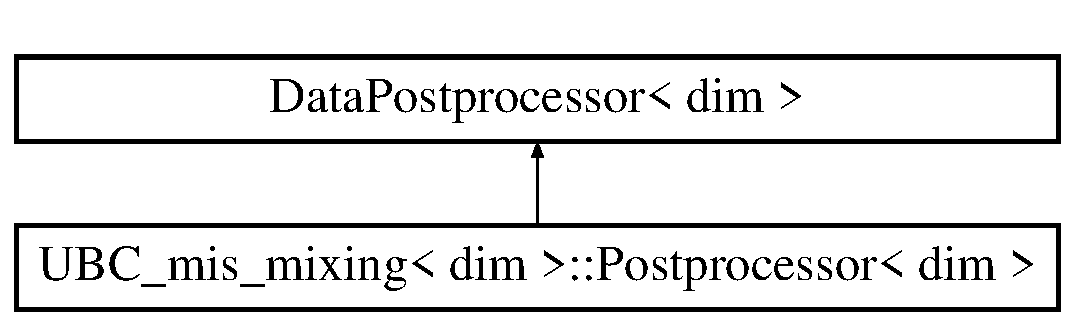
\includegraphics[height=2.000000cm]{class_u_b_c__mis__mixing_1_1_postprocessor}
\end{center}
\end{figure}
\subsubsection*{Public Member Functions}
\begin{DoxyCompactItemize}
\item 
\hyperlink{class_u_b_c__mis__mixing_1_1_postprocessor_ac74c98c423a4fe0dba8f9ef9279c0607}{Postprocessor} (const unsigned int partition)
\item 
virtual void \hyperlink{class_u_b_c__mis__mixing_1_1_postprocessor_ae5ca8f1ef4eb8c682f2c322e7d47b85c}{compute\+\_\+derived\+\_\+quantities\+\_\+vector} (const std\+::vector$<$ Vector$<$ double $>$ $>$ \&uh, const std\+::vector$<$ std\+::vector$<$ Tensor$<$ 1, dim $>$ $>$ $>$ \&duh, const std\+::vector$<$ std\+::vector$<$ Tensor$<$ 2, dim $>$ $>$ $>$ \&dduh, const std\+::vector$<$ Point$<$ dim $>$ $>$ \&normals, const std\+::vector$<$ Point$<$ dim $>$ $>$ \&evaluation\+\_\+points, std\+::vector$<$ Vector$<$ double $>$ $>$ \&computed\+\_\+quantities) const 
\item 
virtual std\+::vector$<$ std\+::string $>$ \hyperlink{class_u_b_c__mis__mixing_1_1_postprocessor_a05ee9a5d6d913c2fe41cb67f9f6f3893}{get\+\_\+names} () const 
\item 
virtual std\+::vector$<$ Data\+Component\+Interpretation\+::\+Data\+Component\+Interpretation $>$ \hyperlink{class_u_b_c__mis__mixing_1_1_postprocessor_a3038fa1744200de88fe27c335ded7a39}{get\+\_\+data\+\_\+component\+\_\+interpretation} () const 
\item 
virtual Update\+Flags \hyperlink{class_u_b_c__mis__mixing_1_1_postprocessor_a002ab5928ee9d405325b9804355ccb9c}{get\+\_\+needed\+\_\+update\+\_\+flags} () const 
\end{DoxyCompactItemize}


\subsubsection{Constructor \& Destructor Documentation}
\hypertarget{class_u_b_c__mis__mixing_1_1_postprocessor_ac74c98c423a4fe0dba8f9ef9279c0607}{}\index{U\+B\+C\+\_\+mis\+\_\+mixing\+::\+Postprocessor@{U\+B\+C\+\_\+mis\+\_\+mixing\+::\+Postprocessor}!Postprocessor@{Postprocessor}}
\index{Postprocessor@{Postprocessor}!U\+B\+C\+\_\+mis\+\_\+mixing\+::\+Postprocessor@{U\+B\+C\+\_\+mis\+\_\+mixing\+::\+Postprocessor}}
\paragraph[{Postprocessor(const unsigned int partition)}]{\setlength{\rightskip}{0pt plus 5cm}template$<$int dim$>$ template$<$int dim$>$ {\bf U\+B\+C\+\_\+mis\+\_\+mixing}$<$ dim $>$\+::{\bf Postprocessor}$<$ dim $>$\+::{\bf Postprocessor} (
\begin{DoxyParamCaption}
\item[{const unsigned int}]{partition}
\end{DoxyParamCaption}
)}\label{class_u_b_c__mis__mixing_1_1_postprocessor_ac74c98c423a4fe0dba8f9ef9279c0607}


\subsubsection{Member Function Documentation}
\hypertarget{class_u_b_c__mis__mixing_1_1_postprocessor_ae5ca8f1ef4eb8c682f2c322e7d47b85c}{}\index{U\+B\+C\+\_\+mis\+\_\+mixing\+::\+Postprocessor@{U\+B\+C\+\_\+mis\+\_\+mixing\+::\+Postprocessor}!compute\+\_\+derived\+\_\+quantities\+\_\+vector@{compute\+\_\+derived\+\_\+quantities\+\_\+vector}}
\index{compute\+\_\+derived\+\_\+quantities\+\_\+vector@{compute\+\_\+derived\+\_\+quantities\+\_\+vector}!U\+B\+C\+\_\+mis\+\_\+mixing\+::\+Postprocessor@{U\+B\+C\+\_\+mis\+\_\+mixing\+::\+Postprocessor}}
\paragraph[{compute\+\_\+derived\+\_\+quantities\+\_\+vector(const std\+::vector$<$ Vector$<$ double $>$ $>$ \&uh, const std\+::vector$<$ std\+::vector$<$ Tensor$<$ 1, dim $>$ $>$ $>$ \&duh, const std\+::vector$<$ std\+::vector$<$ Tensor$<$ 2, dim $>$ $>$ $>$ \&dduh, const std\+::vector$<$ Point$<$ dim $>$ $>$ \&normals, const std\+::vector$<$ Point$<$ dim $>$ $>$ \&evaluation\+\_\+points, std\+::vector$<$ Vector$<$ double $>$ $>$ \&computed\+\_\+quantities) const }]{\setlength{\rightskip}{0pt plus 5cm}template$<$int dim$>$ template$<$int dim$>$ void {\bf U\+B\+C\+\_\+mis\+\_\+mixing}$<$ dim $>$\+::{\bf Postprocessor}$<$ dim $>$\+::compute\+\_\+derived\+\_\+quantities\+\_\+vector (
\begin{DoxyParamCaption}
\item[{const std\+::vector$<$ Vector$<$ double $>$ $>$ \&}]{uh, }
\item[{const std\+::vector$<$ std\+::vector$<$ Tensor$<$ 1, dim $>$ $>$ $>$ \&}]{duh, }
\item[{const std\+::vector$<$ std\+::vector$<$ Tensor$<$ 2, dim $>$ $>$ $>$ \&}]{dduh, }
\item[{const std\+::vector$<$ Point$<$ dim $>$ $>$ \&}]{normals, }
\item[{const std\+::vector$<$ Point$<$ dim $>$ $>$ \&}]{evaluation\+\_\+points, }
\item[{std\+::vector$<$ Vector$<$ double $>$ $>$ \&}]{computed\+\_\+quantities}
\end{DoxyParamCaption}
) const\hspace{0.3cm}{\ttfamily [virtual]}}\label{class_u_b_c__mis__mixing_1_1_postprocessor_ae5ca8f1ef4eb8c682f2c322e7d47b85c}
\hypertarget{class_u_b_c__mis__mixing_1_1_postprocessor_a3038fa1744200de88fe27c335ded7a39}{}\index{U\+B\+C\+\_\+mis\+\_\+mixing\+::\+Postprocessor@{U\+B\+C\+\_\+mis\+\_\+mixing\+::\+Postprocessor}!get\+\_\+data\+\_\+component\+\_\+interpretation@{get\+\_\+data\+\_\+component\+\_\+interpretation}}
\index{get\+\_\+data\+\_\+component\+\_\+interpretation@{get\+\_\+data\+\_\+component\+\_\+interpretation}!U\+B\+C\+\_\+mis\+\_\+mixing\+::\+Postprocessor@{U\+B\+C\+\_\+mis\+\_\+mixing\+::\+Postprocessor}}
\paragraph[{get\+\_\+data\+\_\+component\+\_\+interpretation() const }]{\setlength{\rightskip}{0pt plus 5cm}template$<$int dim$>$ template$<$int dim$>$ std\+::vector$<$ Data\+Component\+Interpretation\+::\+Data\+Component\+Interpretation $>$ {\bf U\+B\+C\+\_\+mis\+\_\+mixing}$<$ dim $>$\+::{\bf Postprocessor}$<$ dim $>$\+::get\+\_\+data\+\_\+component\+\_\+interpretation (
\begin{DoxyParamCaption}
{}
\end{DoxyParamCaption}
) const\hspace{0.3cm}{\ttfamily [virtual]}}\label{class_u_b_c__mis__mixing_1_1_postprocessor_a3038fa1744200de88fe27c335ded7a39}
\hypertarget{class_u_b_c__mis__mixing_1_1_postprocessor_a05ee9a5d6d913c2fe41cb67f9f6f3893}{}\index{U\+B\+C\+\_\+mis\+\_\+mixing\+::\+Postprocessor@{U\+B\+C\+\_\+mis\+\_\+mixing\+::\+Postprocessor}!get\+\_\+names@{get\+\_\+names}}
\index{get\+\_\+names@{get\+\_\+names}!U\+B\+C\+\_\+mis\+\_\+mixing\+::\+Postprocessor@{U\+B\+C\+\_\+mis\+\_\+mixing\+::\+Postprocessor}}
\paragraph[{get\+\_\+names() const }]{\setlength{\rightskip}{0pt plus 5cm}template$<$int dim$>$ template$<$int dim$>$ std\+::vector$<$ std\+::string $>$ {\bf U\+B\+C\+\_\+mis\+\_\+mixing}$<$ dim $>$\+::{\bf Postprocessor}$<$ dim $>$\+::get\+\_\+names (
\begin{DoxyParamCaption}
{}
\end{DoxyParamCaption}
) const\hspace{0.3cm}{\ttfamily [virtual]}}\label{class_u_b_c__mis__mixing_1_1_postprocessor_a05ee9a5d6d913c2fe41cb67f9f6f3893}
\hypertarget{class_u_b_c__mis__mixing_1_1_postprocessor_a002ab5928ee9d405325b9804355ccb9c}{}\index{U\+B\+C\+\_\+mis\+\_\+mixing\+::\+Postprocessor@{U\+B\+C\+\_\+mis\+\_\+mixing\+::\+Postprocessor}!get\+\_\+needed\+\_\+update\+\_\+flags@{get\+\_\+needed\+\_\+update\+\_\+flags}}
\index{get\+\_\+needed\+\_\+update\+\_\+flags@{get\+\_\+needed\+\_\+update\+\_\+flags}!U\+B\+C\+\_\+mis\+\_\+mixing\+::\+Postprocessor@{U\+B\+C\+\_\+mis\+\_\+mixing\+::\+Postprocessor}}
\paragraph[{get\+\_\+needed\+\_\+update\+\_\+flags() const }]{\setlength{\rightskip}{0pt plus 5cm}template$<$int dim$>$ template$<$int dim$>$ Update\+Flags {\bf U\+B\+C\+\_\+mis\+\_\+mixing}$<$ dim $>$\+::{\bf Postprocessor}$<$ dim $>$\+::get\+\_\+needed\+\_\+update\+\_\+flags (
\begin{DoxyParamCaption}
{}
\end{DoxyParamCaption}
) const\hspace{0.3cm}{\ttfamily [virtual]}}\label{class_u_b_c__mis__mixing_1_1_postprocessor_a002ab5928ee9d405325b9804355ccb9c}


The documentation for this class was generated from the following file\+:\begin{DoxyCompactItemize}
\item 
/\+Users/miranus/work/\+Devs/miscible\+\_\+mixing\+\_\+series/miscible\+\_\+mixing/source/post\+\_\+process/\hyperlink{post__processing_8cc}{post\+\_\+processing.\+cc}\end{DoxyCompactItemize}

\hypertarget{struct_assembly_1_1_copy_data_1_1pressure__rot__step}{}\subsection{Assembly\+:\+:Copy\+Data\+:\+:pressure\+\_\+rot\+\_\+step$<$ dim $>$ Struct Template Reference}
\label{struct_assembly_1_1_copy_data_1_1pressure__rot__step}\index{Assembly\+::\+Copy\+Data\+::pressure\+\_\+rot\+\_\+step$<$ dim $>$@{Assembly\+::\+Copy\+Data\+::pressure\+\_\+rot\+\_\+step$<$ dim $>$}}


{\ttfamily \#include $<$assembly\+\_\+copydata.\+h$>$}

\subsubsection*{Public Member Functions}
\begin{DoxyCompactItemize}
\item 
\hyperlink{struct_assembly_1_1_copy_data_1_1pressure__rot__step_add5e474ef4a3a50803ac2e722ef7fc7a}{pressure\+\_\+rot\+\_\+step} (const Finite\+Element$<$ dim $>$ \&fe\+\_\+pressure)
\item 
\hyperlink{struct_assembly_1_1_copy_data_1_1pressure__rot__step_ab2fc649ebf1d5b280883f7e4f62cb4e3}{pressure\+\_\+rot\+\_\+step} (const \hyperlink{struct_assembly_1_1_copy_data_1_1pressure__rot__step}{pressure\+\_\+rot\+\_\+step} \&data)
\end{DoxyCompactItemize}
\subsubsection*{Public Attributes}
\begin{DoxyCompactItemize}
\item 
Full\+Matrix$<$ double $>$ \hyperlink{struct_assembly_1_1_copy_data_1_1pressure__rot__step_a316a4598a7bed63334bcb4699469f366}{local\+\_\+matrix}
\item 
Vector$<$ double $>$ \hyperlink{struct_assembly_1_1_copy_data_1_1pressure__rot__step_a43d09c97e5a67574fd254c7539b8d439}{local\+\_\+rhs}
\item 
std\+::vector$<$ types\+::global\+\_\+dof\+\_\+index $>$ \hyperlink{struct_assembly_1_1_copy_data_1_1pressure__rot__step_ade1a65d97b3092835d27a4cd6295482f}{local\+\_\+dof\+\_\+indices}
\end{DoxyCompactItemize}


\subsubsection{Constructor \& Destructor Documentation}
\hypertarget{struct_assembly_1_1_copy_data_1_1pressure__rot__step_add5e474ef4a3a50803ac2e722ef7fc7a}{}\index{Assembly\+::\+Copy\+Data\+::pressure\+\_\+rot\+\_\+step@{Assembly\+::\+Copy\+Data\+::pressure\+\_\+rot\+\_\+step}!pressure\+\_\+rot\+\_\+step@{pressure\+\_\+rot\+\_\+step}}
\index{pressure\+\_\+rot\+\_\+step@{pressure\+\_\+rot\+\_\+step}!Assembly\+::\+Copy\+Data\+::pressure\+\_\+rot\+\_\+step@{Assembly\+::\+Copy\+Data\+::pressure\+\_\+rot\+\_\+step}}
\paragraph[{pressure\+\_\+rot\+\_\+step(const Finite\+Element$<$ dim $>$ \&fe\+\_\+pressure)}]{\setlength{\rightskip}{0pt plus 5cm}template$<$int dim$>$ {\bf Assembly\+::\+Copy\+Data\+::pressure\+\_\+rot\+\_\+step}$<$ dim $>$\+::{\bf pressure\+\_\+rot\+\_\+step} (
\begin{DoxyParamCaption}
\item[{const Finite\+Element$<$ dim $>$ \&}]{fe\+\_\+pressure}
\end{DoxyParamCaption}
)}\label{struct_assembly_1_1_copy_data_1_1pressure__rot__step_add5e474ef4a3a50803ac2e722ef7fc7a}
\hypertarget{struct_assembly_1_1_copy_data_1_1pressure__rot__step_ab2fc649ebf1d5b280883f7e4f62cb4e3}{}\index{Assembly\+::\+Copy\+Data\+::pressure\+\_\+rot\+\_\+step@{Assembly\+::\+Copy\+Data\+::pressure\+\_\+rot\+\_\+step}!pressure\+\_\+rot\+\_\+step@{pressure\+\_\+rot\+\_\+step}}
\index{pressure\+\_\+rot\+\_\+step@{pressure\+\_\+rot\+\_\+step}!Assembly\+::\+Copy\+Data\+::pressure\+\_\+rot\+\_\+step@{Assembly\+::\+Copy\+Data\+::pressure\+\_\+rot\+\_\+step}}
\paragraph[{pressure\+\_\+rot\+\_\+step(const pressure\+\_\+rot\+\_\+step \&data)}]{\setlength{\rightskip}{0pt plus 5cm}template$<$int dim$>$ {\bf Assembly\+::\+Copy\+Data\+::pressure\+\_\+rot\+\_\+step}$<$ dim $>$\+::{\bf pressure\+\_\+rot\+\_\+step} (
\begin{DoxyParamCaption}
\item[{const {\bf pressure\+\_\+rot\+\_\+step}$<$ dim $>$ \&}]{data}
\end{DoxyParamCaption}
)}\label{struct_assembly_1_1_copy_data_1_1pressure__rot__step_ab2fc649ebf1d5b280883f7e4f62cb4e3}


\subsubsection{Member Data Documentation}
\hypertarget{struct_assembly_1_1_copy_data_1_1pressure__rot__step_ade1a65d97b3092835d27a4cd6295482f}{}\index{Assembly\+::\+Copy\+Data\+::pressure\+\_\+rot\+\_\+step@{Assembly\+::\+Copy\+Data\+::pressure\+\_\+rot\+\_\+step}!local\+\_\+dof\+\_\+indices@{local\+\_\+dof\+\_\+indices}}
\index{local\+\_\+dof\+\_\+indices@{local\+\_\+dof\+\_\+indices}!Assembly\+::\+Copy\+Data\+::pressure\+\_\+rot\+\_\+step@{Assembly\+::\+Copy\+Data\+::pressure\+\_\+rot\+\_\+step}}
\paragraph[{local\+\_\+dof\+\_\+indices}]{\setlength{\rightskip}{0pt plus 5cm}template$<$int dim$>$ std\+::vector$<$types\+::global\+\_\+dof\+\_\+index$>$ {\bf Assembly\+::\+Copy\+Data\+::pressure\+\_\+rot\+\_\+step}$<$ dim $>$\+::local\+\_\+dof\+\_\+indices}\label{struct_assembly_1_1_copy_data_1_1pressure__rot__step_ade1a65d97b3092835d27a4cd6295482f}
\hypertarget{struct_assembly_1_1_copy_data_1_1pressure__rot__step_a316a4598a7bed63334bcb4699469f366}{}\index{Assembly\+::\+Copy\+Data\+::pressure\+\_\+rot\+\_\+step@{Assembly\+::\+Copy\+Data\+::pressure\+\_\+rot\+\_\+step}!local\+\_\+matrix@{local\+\_\+matrix}}
\index{local\+\_\+matrix@{local\+\_\+matrix}!Assembly\+::\+Copy\+Data\+::pressure\+\_\+rot\+\_\+step@{Assembly\+::\+Copy\+Data\+::pressure\+\_\+rot\+\_\+step}}
\paragraph[{local\+\_\+matrix}]{\setlength{\rightskip}{0pt plus 5cm}template$<$int dim$>$ Full\+Matrix$<$double$>$ {\bf Assembly\+::\+Copy\+Data\+::pressure\+\_\+rot\+\_\+step}$<$ dim $>$\+::local\+\_\+matrix}\label{struct_assembly_1_1_copy_data_1_1pressure__rot__step_a316a4598a7bed63334bcb4699469f366}
\hypertarget{struct_assembly_1_1_copy_data_1_1pressure__rot__step_a43d09c97e5a67574fd254c7539b8d439}{}\index{Assembly\+::\+Copy\+Data\+::pressure\+\_\+rot\+\_\+step@{Assembly\+::\+Copy\+Data\+::pressure\+\_\+rot\+\_\+step}!local\+\_\+rhs@{local\+\_\+rhs}}
\index{local\+\_\+rhs@{local\+\_\+rhs}!Assembly\+::\+Copy\+Data\+::pressure\+\_\+rot\+\_\+step@{Assembly\+::\+Copy\+Data\+::pressure\+\_\+rot\+\_\+step}}
\paragraph[{local\+\_\+rhs}]{\setlength{\rightskip}{0pt plus 5cm}template$<$int dim$>$ Vector$<$double$>$ {\bf Assembly\+::\+Copy\+Data\+::pressure\+\_\+rot\+\_\+step}$<$ dim $>$\+::local\+\_\+rhs}\label{struct_assembly_1_1_copy_data_1_1pressure__rot__step_a43d09c97e5a67574fd254c7539b8d439}


The documentation for this struct was generated from the following file\+:\begin{DoxyCompactItemize}
\item 
/\+Users/miranus/work/\+Devs/miscible\+\_\+mixing\+\_\+series/miscible\+\_\+mixing/include/mismix/\hyperlink{assembly__copydata_8h}{assembly\+\_\+copydata.\+h}\end{DoxyCompactItemize}

\hypertarget{struct_assembly_1_1_scratch_1_1pressure__rot__step}{}\subsection{Assembly\+:\+:Scratch\+:\+:pressure\+\_\+rot\+\_\+step$<$ dim $>$ Struct Template Reference}
\label{struct_assembly_1_1_scratch_1_1pressure__rot__step}\index{Assembly\+::\+Scratch\+::pressure\+\_\+rot\+\_\+step$<$ dim $>$@{Assembly\+::\+Scratch\+::pressure\+\_\+rot\+\_\+step$<$ dim $>$}}


{\ttfamily \#include $<$assembly\+\_\+copydata.\+h$>$}

\subsubsection*{Public Member Functions}
\begin{DoxyCompactItemize}
\item 
\hyperlink{struct_assembly_1_1_scratch_1_1pressure__rot__step_a9a782a85d4cfb0b5f50a0fcd76924d23}{pressure\+\_\+rot\+\_\+step} (const Finite\+Element$<$ dim $>$ \&fe\+\_\+pressure, const Mapping$<$ dim $>$ \&pressure\+\_\+mapping, const Quadrature$<$ dim $>$ \&quadrature, const Update\+Flags pressure\+\_\+update\+\_\+flags, const Finite\+Element$<$ dim $>$ \&fe\+\_\+velocity, const Mapping$<$ dim $>$ \&velocity\+\_\+mapping, const Update\+Flags velocity\+\_\+update\+\_\+flags, const Finite\+Element$<$ dim $>$ \&concentr\+\_\+fe, const Mapping$<$ dim $>$ \&concentr\+\_\+mapping, const Update\+Flags concentr\+\_\+update\+\_\+flags)
\item 
\hyperlink{struct_assembly_1_1_scratch_1_1pressure__rot__step_ad8ce0533193a2013774b98c0e7b81581}{pressure\+\_\+rot\+\_\+step} (const \hyperlink{struct_assembly_1_1_scratch_1_1pressure__rot__step}{pressure\+\_\+rot\+\_\+step} \&data)
\end{DoxyCompactItemize}
\subsubsection*{Public Attributes}
\begin{DoxyCompactItemize}
\item 
F\+E\+Values$<$ dim $>$ \hyperlink{struct_assembly_1_1_scratch_1_1pressure__rot__step_ac41f7bf5aa82b80e01ba8453c31e5fdd}{fe\+\_\+pressure\+\_\+values}
\item 
F\+E\+Values$<$ dim $>$ \hyperlink{struct_assembly_1_1_scratch_1_1pressure__rot__step_af0e05e66de3967bf2736defbcee157d5}{fe\+\_\+velocity\+\_\+values}
\item 
F\+E\+Values$<$ dim $>$ \hyperlink{struct_assembly_1_1_scratch_1_1pressure__rot__step_a897061bf69830b1212f797ff3af9d250}{concentr\+\_\+fe\+\_\+values}
\item 
std\+::vector$<$ double $>$ \hyperlink{struct_assembly_1_1_scratch_1_1pressure__rot__step_aeaca955234a85e889b5c71e912240025}{phi\+\_\+p}
\item 
std\+::vector$<$ double $>$ \hyperlink{struct_assembly_1_1_scratch_1_1pressure__rot__step_abd85718af16840d6abc3a01abe1fb6e3}{aux\+\_\+sol\+\_\+values}
\item 
std\+::vector$<$ double $>$ \hyperlink{struct_assembly_1_1_scratch_1_1pressure__rot__step_a9de7969f5b98cb8dfc629301647b5c3e}{pre\+\_\+sol\+\_\+values}
\item 
std\+::vector$<$ Tensor$<$ 2, dim $>$ $>$ \hyperlink{struct_assembly_1_1_scratch_1_1pressure__rot__step_a8530984bbf6ea328b90cf347b748bdc6}{grad\+\_\+vel\+\_\+sol\+\_\+values}
\item 
std\+::vector$<$ double $>$ \hyperlink{struct_assembly_1_1_scratch_1_1pressure__rot__step_a80d0030ad6c786b9d1e7e5365497ac41}{concentr\+\_\+values}
\item 
std\+::vector$<$ Symmetric\+Tensor$<$ 2, dim $>$ $>$ \hyperlink{struct_assembly_1_1_scratch_1_1pressure__rot__step_a1bfe900ee774329a556f620ae765573b}{symm\+\_\+grads\+\_\+vel\+\_\+sol}
\end{DoxyCompactItemize}


\subsubsection{Constructor \& Destructor Documentation}
\hypertarget{struct_assembly_1_1_scratch_1_1pressure__rot__step_a9a782a85d4cfb0b5f50a0fcd76924d23}{}\index{Assembly\+::\+Scratch\+::pressure\+\_\+rot\+\_\+step@{Assembly\+::\+Scratch\+::pressure\+\_\+rot\+\_\+step}!pressure\+\_\+rot\+\_\+step@{pressure\+\_\+rot\+\_\+step}}
\index{pressure\+\_\+rot\+\_\+step@{pressure\+\_\+rot\+\_\+step}!Assembly\+::\+Scratch\+::pressure\+\_\+rot\+\_\+step@{Assembly\+::\+Scratch\+::pressure\+\_\+rot\+\_\+step}}
\paragraph[{pressure\+\_\+rot\+\_\+step(const Finite\+Element$<$ dim $>$ \&fe\+\_\+pressure, const Mapping$<$ dim $>$ \&pressure\+\_\+mapping, const Quadrature$<$ dim $>$ \&quadrature, const Update\+Flags pressure\+\_\+update\+\_\+flags, const Finite\+Element$<$ dim $>$ \&fe\+\_\+velocity, const Mapping$<$ dim $>$ \&velocity\+\_\+mapping, const Update\+Flags velocity\+\_\+update\+\_\+flags, const Finite\+Element$<$ dim $>$ \&concentr\+\_\+fe, const Mapping$<$ dim $>$ \&concentr\+\_\+mapping, const Update\+Flags concentr\+\_\+update\+\_\+flags)}]{\setlength{\rightskip}{0pt plus 5cm}template$<$int dim$>$ {\bf Assembly\+::\+Scratch\+::pressure\+\_\+rot\+\_\+step}$<$ dim $>$\+::{\bf pressure\+\_\+rot\+\_\+step} (
\begin{DoxyParamCaption}
\item[{const Finite\+Element$<$ dim $>$ \&}]{fe\+\_\+pressure, }
\item[{const Mapping$<$ dim $>$ \&}]{pressure\+\_\+mapping, }
\item[{const Quadrature$<$ dim $>$ \&}]{quadrature, }
\item[{const Update\+Flags}]{pressure\+\_\+update\+\_\+flags, }
\item[{const Finite\+Element$<$ dim $>$ \&}]{fe\+\_\+velocity, }
\item[{const Mapping$<$ dim $>$ \&}]{velocity\+\_\+mapping, }
\item[{const Update\+Flags}]{velocity\+\_\+update\+\_\+flags, }
\item[{const Finite\+Element$<$ dim $>$ \&}]{concentr\+\_\+fe, }
\item[{const Mapping$<$ dim $>$ \&}]{concentr\+\_\+mapping, }
\item[{const Update\+Flags}]{concentr\+\_\+update\+\_\+flags}
\end{DoxyParamCaption}
)}\label{struct_assembly_1_1_scratch_1_1pressure__rot__step_a9a782a85d4cfb0b5f50a0fcd76924d23}
\hypertarget{struct_assembly_1_1_scratch_1_1pressure__rot__step_ad8ce0533193a2013774b98c0e7b81581}{}\index{Assembly\+::\+Scratch\+::pressure\+\_\+rot\+\_\+step@{Assembly\+::\+Scratch\+::pressure\+\_\+rot\+\_\+step}!pressure\+\_\+rot\+\_\+step@{pressure\+\_\+rot\+\_\+step}}
\index{pressure\+\_\+rot\+\_\+step@{pressure\+\_\+rot\+\_\+step}!Assembly\+::\+Scratch\+::pressure\+\_\+rot\+\_\+step@{Assembly\+::\+Scratch\+::pressure\+\_\+rot\+\_\+step}}
\paragraph[{pressure\+\_\+rot\+\_\+step(const pressure\+\_\+rot\+\_\+step \&data)}]{\setlength{\rightskip}{0pt plus 5cm}template$<$int dim$>$ {\bf Assembly\+::\+Scratch\+::pressure\+\_\+rot\+\_\+step}$<$ dim $>$\+::{\bf pressure\+\_\+rot\+\_\+step} (
\begin{DoxyParamCaption}
\item[{const {\bf pressure\+\_\+rot\+\_\+step}$<$ dim $>$ \&}]{data}
\end{DoxyParamCaption}
)}\label{struct_assembly_1_1_scratch_1_1pressure__rot__step_ad8ce0533193a2013774b98c0e7b81581}


\subsubsection{Member Data Documentation}
\hypertarget{struct_assembly_1_1_scratch_1_1pressure__rot__step_abd85718af16840d6abc3a01abe1fb6e3}{}\index{Assembly\+::\+Scratch\+::pressure\+\_\+rot\+\_\+step@{Assembly\+::\+Scratch\+::pressure\+\_\+rot\+\_\+step}!aux\+\_\+sol\+\_\+values@{aux\+\_\+sol\+\_\+values}}
\index{aux\+\_\+sol\+\_\+values@{aux\+\_\+sol\+\_\+values}!Assembly\+::\+Scratch\+::pressure\+\_\+rot\+\_\+step@{Assembly\+::\+Scratch\+::pressure\+\_\+rot\+\_\+step}}
\paragraph[{aux\+\_\+sol\+\_\+values}]{\setlength{\rightskip}{0pt plus 5cm}template$<$int dim$>$ std\+::vector$<$double$>$ {\bf Assembly\+::\+Scratch\+::pressure\+\_\+rot\+\_\+step}$<$ dim $>$\+::aux\+\_\+sol\+\_\+values}\label{struct_assembly_1_1_scratch_1_1pressure__rot__step_abd85718af16840d6abc3a01abe1fb6e3}
\hypertarget{struct_assembly_1_1_scratch_1_1pressure__rot__step_a897061bf69830b1212f797ff3af9d250}{}\index{Assembly\+::\+Scratch\+::pressure\+\_\+rot\+\_\+step@{Assembly\+::\+Scratch\+::pressure\+\_\+rot\+\_\+step}!concentr\+\_\+fe\+\_\+values@{concentr\+\_\+fe\+\_\+values}}
\index{concentr\+\_\+fe\+\_\+values@{concentr\+\_\+fe\+\_\+values}!Assembly\+::\+Scratch\+::pressure\+\_\+rot\+\_\+step@{Assembly\+::\+Scratch\+::pressure\+\_\+rot\+\_\+step}}
\paragraph[{concentr\+\_\+fe\+\_\+values}]{\setlength{\rightskip}{0pt plus 5cm}template$<$int dim$>$ F\+E\+Values$<$dim$>$ {\bf Assembly\+::\+Scratch\+::pressure\+\_\+rot\+\_\+step}$<$ dim $>$\+::concentr\+\_\+fe\+\_\+values}\label{struct_assembly_1_1_scratch_1_1pressure__rot__step_a897061bf69830b1212f797ff3af9d250}
\hypertarget{struct_assembly_1_1_scratch_1_1pressure__rot__step_a80d0030ad6c786b9d1e7e5365497ac41}{}\index{Assembly\+::\+Scratch\+::pressure\+\_\+rot\+\_\+step@{Assembly\+::\+Scratch\+::pressure\+\_\+rot\+\_\+step}!concentr\+\_\+values@{concentr\+\_\+values}}
\index{concentr\+\_\+values@{concentr\+\_\+values}!Assembly\+::\+Scratch\+::pressure\+\_\+rot\+\_\+step@{Assembly\+::\+Scratch\+::pressure\+\_\+rot\+\_\+step}}
\paragraph[{concentr\+\_\+values}]{\setlength{\rightskip}{0pt plus 5cm}template$<$int dim$>$ std\+::vector$<$double$>$ {\bf Assembly\+::\+Scratch\+::pressure\+\_\+rot\+\_\+step}$<$ dim $>$\+::concentr\+\_\+values}\label{struct_assembly_1_1_scratch_1_1pressure__rot__step_a80d0030ad6c786b9d1e7e5365497ac41}
\hypertarget{struct_assembly_1_1_scratch_1_1pressure__rot__step_ac41f7bf5aa82b80e01ba8453c31e5fdd}{}\index{Assembly\+::\+Scratch\+::pressure\+\_\+rot\+\_\+step@{Assembly\+::\+Scratch\+::pressure\+\_\+rot\+\_\+step}!fe\+\_\+pressure\+\_\+values@{fe\+\_\+pressure\+\_\+values}}
\index{fe\+\_\+pressure\+\_\+values@{fe\+\_\+pressure\+\_\+values}!Assembly\+::\+Scratch\+::pressure\+\_\+rot\+\_\+step@{Assembly\+::\+Scratch\+::pressure\+\_\+rot\+\_\+step}}
\paragraph[{fe\+\_\+pressure\+\_\+values}]{\setlength{\rightskip}{0pt plus 5cm}template$<$int dim$>$ F\+E\+Values$<$dim$>$ {\bf Assembly\+::\+Scratch\+::pressure\+\_\+rot\+\_\+step}$<$ dim $>$\+::fe\+\_\+pressure\+\_\+values}\label{struct_assembly_1_1_scratch_1_1pressure__rot__step_ac41f7bf5aa82b80e01ba8453c31e5fdd}
\hypertarget{struct_assembly_1_1_scratch_1_1pressure__rot__step_af0e05e66de3967bf2736defbcee157d5}{}\index{Assembly\+::\+Scratch\+::pressure\+\_\+rot\+\_\+step@{Assembly\+::\+Scratch\+::pressure\+\_\+rot\+\_\+step}!fe\+\_\+velocity\+\_\+values@{fe\+\_\+velocity\+\_\+values}}
\index{fe\+\_\+velocity\+\_\+values@{fe\+\_\+velocity\+\_\+values}!Assembly\+::\+Scratch\+::pressure\+\_\+rot\+\_\+step@{Assembly\+::\+Scratch\+::pressure\+\_\+rot\+\_\+step}}
\paragraph[{fe\+\_\+velocity\+\_\+values}]{\setlength{\rightskip}{0pt plus 5cm}template$<$int dim$>$ F\+E\+Values$<$dim$>$ {\bf Assembly\+::\+Scratch\+::pressure\+\_\+rot\+\_\+step}$<$ dim $>$\+::fe\+\_\+velocity\+\_\+values}\label{struct_assembly_1_1_scratch_1_1pressure__rot__step_af0e05e66de3967bf2736defbcee157d5}
\hypertarget{struct_assembly_1_1_scratch_1_1pressure__rot__step_a8530984bbf6ea328b90cf347b748bdc6}{}\index{Assembly\+::\+Scratch\+::pressure\+\_\+rot\+\_\+step@{Assembly\+::\+Scratch\+::pressure\+\_\+rot\+\_\+step}!grad\+\_\+vel\+\_\+sol\+\_\+values@{grad\+\_\+vel\+\_\+sol\+\_\+values}}
\index{grad\+\_\+vel\+\_\+sol\+\_\+values@{grad\+\_\+vel\+\_\+sol\+\_\+values}!Assembly\+::\+Scratch\+::pressure\+\_\+rot\+\_\+step@{Assembly\+::\+Scratch\+::pressure\+\_\+rot\+\_\+step}}
\paragraph[{grad\+\_\+vel\+\_\+sol\+\_\+values}]{\setlength{\rightskip}{0pt plus 5cm}template$<$int dim$>$ std\+::vector$<$Tensor$<$2,dim$>$ $>$ {\bf Assembly\+::\+Scratch\+::pressure\+\_\+rot\+\_\+step}$<$ dim $>$\+::grad\+\_\+vel\+\_\+sol\+\_\+values}\label{struct_assembly_1_1_scratch_1_1pressure__rot__step_a8530984bbf6ea328b90cf347b748bdc6}
\hypertarget{struct_assembly_1_1_scratch_1_1pressure__rot__step_aeaca955234a85e889b5c71e912240025}{}\index{Assembly\+::\+Scratch\+::pressure\+\_\+rot\+\_\+step@{Assembly\+::\+Scratch\+::pressure\+\_\+rot\+\_\+step}!phi\+\_\+p@{phi\+\_\+p}}
\index{phi\+\_\+p@{phi\+\_\+p}!Assembly\+::\+Scratch\+::pressure\+\_\+rot\+\_\+step@{Assembly\+::\+Scratch\+::pressure\+\_\+rot\+\_\+step}}
\paragraph[{phi\+\_\+p}]{\setlength{\rightskip}{0pt plus 5cm}template$<$int dim$>$ std\+::vector$<$double$>$ {\bf Assembly\+::\+Scratch\+::pressure\+\_\+rot\+\_\+step}$<$ dim $>$\+::phi\+\_\+p}\label{struct_assembly_1_1_scratch_1_1pressure__rot__step_aeaca955234a85e889b5c71e912240025}
\hypertarget{struct_assembly_1_1_scratch_1_1pressure__rot__step_a9de7969f5b98cb8dfc629301647b5c3e}{}\index{Assembly\+::\+Scratch\+::pressure\+\_\+rot\+\_\+step@{Assembly\+::\+Scratch\+::pressure\+\_\+rot\+\_\+step}!pre\+\_\+sol\+\_\+values@{pre\+\_\+sol\+\_\+values}}
\index{pre\+\_\+sol\+\_\+values@{pre\+\_\+sol\+\_\+values}!Assembly\+::\+Scratch\+::pressure\+\_\+rot\+\_\+step@{Assembly\+::\+Scratch\+::pressure\+\_\+rot\+\_\+step}}
\paragraph[{pre\+\_\+sol\+\_\+values}]{\setlength{\rightskip}{0pt plus 5cm}template$<$int dim$>$ std\+::vector$<$double$>$ {\bf Assembly\+::\+Scratch\+::pressure\+\_\+rot\+\_\+step}$<$ dim $>$\+::pre\+\_\+sol\+\_\+values}\label{struct_assembly_1_1_scratch_1_1pressure__rot__step_a9de7969f5b98cb8dfc629301647b5c3e}
\hypertarget{struct_assembly_1_1_scratch_1_1pressure__rot__step_a1bfe900ee774329a556f620ae765573b}{}\index{Assembly\+::\+Scratch\+::pressure\+\_\+rot\+\_\+step@{Assembly\+::\+Scratch\+::pressure\+\_\+rot\+\_\+step}!symm\+\_\+grads\+\_\+vel\+\_\+sol@{symm\+\_\+grads\+\_\+vel\+\_\+sol}}
\index{symm\+\_\+grads\+\_\+vel\+\_\+sol@{symm\+\_\+grads\+\_\+vel\+\_\+sol}!Assembly\+::\+Scratch\+::pressure\+\_\+rot\+\_\+step@{Assembly\+::\+Scratch\+::pressure\+\_\+rot\+\_\+step}}
\paragraph[{symm\+\_\+grads\+\_\+vel\+\_\+sol}]{\setlength{\rightskip}{0pt plus 5cm}template$<$int dim$>$ std\+::vector$<$Symmetric\+Tensor$<$2,dim$>$ $>$ {\bf Assembly\+::\+Scratch\+::pressure\+\_\+rot\+\_\+step}$<$ dim $>$\+::symm\+\_\+grads\+\_\+vel\+\_\+sol}\label{struct_assembly_1_1_scratch_1_1pressure__rot__step_a1bfe900ee774329a556f620ae765573b}


The documentation for this struct was generated from the following file\+:\begin{DoxyCompactItemize}
\item 
/\+Users/miranus/work/\+Devs/miscible\+\_\+mixing\+\_\+series/miscible\+\_\+mixing/include/mismix/\hyperlink{assembly__copydata_8h}{assembly\+\_\+copydata.\+h}\end{DoxyCompactItemize}

\hypertarget{struct_assembly_1_1_scratch_1_1projection__step}{}\subsection{Assembly\+:\+:Scratch\+:\+:projection\+\_\+step$<$ dim $>$ Struct Template Reference}
\label{struct_assembly_1_1_scratch_1_1projection__step}\index{Assembly\+::\+Scratch\+::projection\+\_\+step$<$ dim $>$@{Assembly\+::\+Scratch\+::projection\+\_\+step$<$ dim $>$}}


{\ttfamily \#include $<$assembly\+\_\+copydata.\+h$>$}

\subsubsection*{Public Member Functions}
\begin{DoxyCompactItemize}
\item 
\hyperlink{struct_assembly_1_1_scratch_1_1projection__step_ab68aa92ddfce17896f9bb3088cd707fc}{projection\+\_\+step} (const Finite\+Element$<$ dim $>$ \&fe\+\_\+auxilary, const Mapping$<$ dim $>$ \&auxilary\+\_\+mapping, const Quadrature$<$ dim $>$ \&quadrature, const Update\+Flags auxilary\+\_\+update\+\_\+flags, const Finite\+Element$<$ dim $>$ \&fe\+\_\+velocity, const Mapping$<$ dim $>$ \&velocity\+\_\+mapping, const Update\+Flags velocity\+\_\+update\+\_\+flags, const Finite\+Element$<$ dim $>$ \&concentr\+\_\+fe, const Mapping$<$ dim $>$ \&concentr\+\_\+mapping, const Update\+Flags concentr\+\_\+update\+\_\+flags)
\item 
\hyperlink{struct_assembly_1_1_scratch_1_1projection__step_aadd897036cbaca7f3a37e3c0b0289bbc}{projection\+\_\+step} (const \hyperlink{struct_assembly_1_1_scratch_1_1projection__step}{projection\+\_\+step} \&data)
\end{DoxyCompactItemize}
\subsubsection*{Public Attributes}
\begin{DoxyCompactItemize}
\item 
F\+E\+Values$<$ dim $>$ \hyperlink{struct_assembly_1_1_scratch_1_1projection__step_a3b5a0afe1eaf675d173af8ffd7663e29}{fe\+\_\+auxilary\+\_\+values}
\item 
F\+E\+Values$<$ dim $>$ \hyperlink{struct_assembly_1_1_scratch_1_1projection__step_af91b8e433a9a308d66f5cbdbc2dd5a7b}{fe\+\_\+velocity\+\_\+values}
\item 
F\+E\+Values$<$ dim $>$ \hyperlink{struct_assembly_1_1_scratch_1_1projection__step_afeebd89eb59befac5386d69841c490b0}{concentr\+\_\+fe\+\_\+values}
\item 
std\+::vector$<$ Tensor$<$ 1, dim $>$ $>$ \hyperlink{struct_assembly_1_1_scratch_1_1projection__step_a75ecf1c6d8aa564824cc3b3376ca08f9}{grads\+\_\+phi\+\_\+p}
\item 
std\+::vector$<$ double $>$ \hyperlink{struct_assembly_1_1_scratch_1_1projection__step_a766727128326d33ecd414c713f186540}{phi\+\_\+p}
\item 
std\+::vector$<$ Tensor$<$ 2, dim $>$ $>$ \hyperlink{struct_assembly_1_1_scratch_1_1projection__step_abc3d9d363dff0cc1bbf8631afc2c777a}{grad\+\_\+vel\+\_\+n\+\_\+plus\+\_\+1\+\_\+values}
\item 
std\+::vector$<$ double $>$ \hyperlink{struct_assembly_1_1_scratch_1_1projection__step_a7907e0ef2eddf65f20a86cc8afff9b66}{concentr\+\_\+values}
\item 
std\+::vector$<$ double $>$ \hyperlink{struct_assembly_1_1_scratch_1_1projection__step_a65701cc9156422035628e7a65783587f}{div\+\_\+vel\+\_\+values}
\end{DoxyCompactItemize}


\subsubsection{Constructor \& Destructor Documentation}
\hypertarget{struct_assembly_1_1_scratch_1_1projection__step_ab68aa92ddfce17896f9bb3088cd707fc}{}\index{Assembly\+::\+Scratch\+::projection\+\_\+step@{Assembly\+::\+Scratch\+::projection\+\_\+step}!projection\+\_\+step@{projection\+\_\+step}}
\index{projection\+\_\+step@{projection\+\_\+step}!Assembly\+::\+Scratch\+::projection\+\_\+step@{Assembly\+::\+Scratch\+::projection\+\_\+step}}
\paragraph[{projection\+\_\+step(const Finite\+Element$<$ dim $>$ \&fe\+\_\+auxilary, const Mapping$<$ dim $>$ \&auxilary\+\_\+mapping, const Quadrature$<$ dim $>$ \&quadrature, const Update\+Flags auxilary\+\_\+update\+\_\+flags, const Finite\+Element$<$ dim $>$ \&fe\+\_\+velocity, const Mapping$<$ dim $>$ \&velocity\+\_\+mapping, const Update\+Flags velocity\+\_\+update\+\_\+flags, const Finite\+Element$<$ dim $>$ \&concentr\+\_\+fe, const Mapping$<$ dim $>$ \&concentr\+\_\+mapping, const Update\+Flags concentr\+\_\+update\+\_\+flags)}]{\setlength{\rightskip}{0pt plus 5cm}template$<$int dim$>$ {\bf Assembly\+::\+Scratch\+::projection\+\_\+step}$<$ dim $>$\+::{\bf projection\+\_\+step} (
\begin{DoxyParamCaption}
\item[{const Finite\+Element$<$ dim $>$ \&}]{fe\+\_\+auxilary, }
\item[{const Mapping$<$ dim $>$ \&}]{auxilary\+\_\+mapping, }
\item[{const Quadrature$<$ dim $>$ \&}]{quadrature, }
\item[{const Update\+Flags}]{auxilary\+\_\+update\+\_\+flags, }
\item[{const Finite\+Element$<$ dim $>$ \&}]{fe\+\_\+velocity, }
\item[{const Mapping$<$ dim $>$ \&}]{velocity\+\_\+mapping, }
\item[{const Update\+Flags}]{velocity\+\_\+update\+\_\+flags, }
\item[{const Finite\+Element$<$ dim $>$ \&}]{concentr\+\_\+fe, }
\item[{const Mapping$<$ dim $>$ \&}]{concentr\+\_\+mapping, }
\item[{const Update\+Flags}]{concentr\+\_\+update\+\_\+flags}
\end{DoxyParamCaption}
)}\label{struct_assembly_1_1_scratch_1_1projection__step_ab68aa92ddfce17896f9bb3088cd707fc}
\hypertarget{struct_assembly_1_1_scratch_1_1projection__step_aadd897036cbaca7f3a37e3c0b0289bbc}{}\index{Assembly\+::\+Scratch\+::projection\+\_\+step@{Assembly\+::\+Scratch\+::projection\+\_\+step}!projection\+\_\+step@{projection\+\_\+step}}
\index{projection\+\_\+step@{projection\+\_\+step}!Assembly\+::\+Scratch\+::projection\+\_\+step@{Assembly\+::\+Scratch\+::projection\+\_\+step}}
\paragraph[{projection\+\_\+step(const projection\+\_\+step \&data)}]{\setlength{\rightskip}{0pt plus 5cm}template$<$int dim$>$ {\bf Assembly\+::\+Scratch\+::projection\+\_\+step}$<$ dim $>$\+::{\bf projection\+\_\+step} (
\begin{DoxyParamCaption}
\item[{const {\bf projection\+\_\+step}$<$ dim $>$ \&}]{data}
\end{DoxyParamCaption}
)}\label{struct_assembly_1_1_scratch_1_1projection__step_aadd897036cbaca7f3a37e3c0b0289bbc}


\subsubsection{Member Data Documentation}
\hypertarget{struct_assembly_1_1_scratch_1_1projection__step_afeebd89eb59befac5386d69841c490b0}{}\index{Assembly\+::\+Scratch\+::projection\+\_\+step@{Assembly\+::\+Scratch\+::projection\+\_\+step}!concentr\+\_\+fe\+\_\+values@{concentr\+\_\+fe\+\_\+values}}
\index{concentr\+\_\+fe\+\_\+values@{concentr\+\_\+fe\+\_\+values}!Assembly\+::\+Scratch\+::projection\+\_\+step@{Assembly\+::\+Scratch\+::projection\+\_\+step}}
\paragraph[{concentr\+\_\+fe\+\_\+values}]{\setlength{\rightskip}{0pt plus 5cm}template$<$int dim$>$ F\+E\+Values$<$dim$>$ {\bf Assembly\+::\+Scratch\+::projection\+\_\+step}$<$ dim $>$\+::concentr\+\_\+fe\+\_\+values}\label{struct_assembly_1_1_scratch_1_1projection__step_afeebd89eb59befac5386d69841c490b0}
\hypertarget{struct_assembly_1_1_scratch_1_1projection__step_a7907e0ef2eddf65f20a86cc8afff9b66}{}\index{Assembly\+::\+Scratch\+::projection\+\_\+step@{Assembly\+::\+Scratch\+::projection\+\_\+step}!concentr\+\_\+values@{concentr\+\_\+values}}
\index{concentr\+\_\+values@{concentr\+\_\+values}!Assembly\+::\+Scratch\+::projection\+\_\+step@{Assembly\+::\+Scratch\+::projection\+\_\+step}}
\paragraph[{concentr\+\_\+values}]{\setlength{\rightskip}{0pt plus 5cm}template$<$int dim$>$ std\+::vector$<$double$>$ {\bf Assembly\+::\+Scratch\+::projection\+\_\+step}$<$ dim $>$\+::concentr\+\_\+values}\label{struct_assembly_1_1_scratch_1_1projection__step_a7907e0ef2eddf65f20a86cc8afff9b66}
\hypertarget{struct_assembly_1_1_scratch_1_1projection__step_a65701cc9156422035628e7a65783587f}{}\index{Assembly\+::\+Scratch\+::projection\+\_\+step@{Assembly\+::\+Scratch\+::projection\+\_\+step}!div\+\_\+vel\+\_\+values@{div\+\_\+vel\+\_\+values}}
\index{div\+\_\+vel\+\_\+values@{div\+\_\+vel\+\_\+values}!Assembly\+::\+Scratch\+::projection\+\_\+step@{Assembly\+::\+Scratch\+::projection\+\_\+step}}
\paragraph[{div\+\_\+vel\+\_\+values}]{\setlength{\rightskip}{0pt plus 5cm}template$<$int dim$>$ std\+::vector$<$double$>$ {\bf Assembly\+::\+Scratch\+::projection\+\_\+step}$<$ dim $>$\+::div\+\_\+vel\+\_\+values}\label{struct_assembly_1_1_scratch_1_1projection__step_a65701cc9156422035628e7a65783587f}
\hypertarget{struct_assembly_1_1_scratch_1_1projection__step_a3b5a0afe1eaf675d173af8ffd7663e29}{}\index{Assembly\+::\+Scratch\+::projection\+\_\+step@{Assembly\+::\+Scratch\+::projection\+\_\+step}!fe\+\_\+auxilary\+\_\+values@{fe\+\_\+auxilary\+\_\+values}}
\index{fe\+\_\+auxilary\+\_\+values@{fe\+\_\+auxilary\+\_\+values}!Assembly\+::\+Scratch\+::projection\+\_\+step@{Assembly\+::\+Scratch\+::projection\+\_\+step}}
\paragraph[{fe\+\_\+auxilary\+\_\+values}]{\setlength{\rightskip}{0pt plus 5cm}template$<$int dim$>$ F\+E\+Values$<$dim$>$ {\bf Assembly\+::\+Scratch\+::projection\+\_\+step}$<$ dim $>$\+::fe\+\_\+auxilary\+\_\+values}\label{struct_assembly_1_1_scratch_1_1projection__step_a3b5a0afe1eaf675d173af8ffd7663e29}
\hypertarget{struct_assembly_1_1_scratch_1_1projection__step_af91b8e433a9a308d66f5cbdbc2dd5a7b}{}\index{Assembly\+::\+Scratch\+::projection\+\_\+step@{Assembly\+::\+Scratch\+::projection\+\_\+step}!fe\+\_\+velocity\+\_\+values@{fe\+\_\+velocity\+\_\+values}}
\index{fe\+\_\+velocity\+\_\+values@{fe\+\_\+velocity\+\_\+values}!Assembly\+::\+Scratch\+::projection\+\_\+step@{Assembly\+::\+Scratch\+::projection\+\_\+step}}
\paragraph[{fe\+\_\+velocity\+\_\+values}]{\setlength{\rightskip}{0pt plus 5cm}template$<$int dim$>$ F\+E\+Values$<$dim$>$ {\bf Assembly\+::\+Scratch\+::projection\+\_\+step}$<$ dim $>$\+::fe\+\_\+velocity\+\_\+values}\label{struct_assembly_1_1_scratch_1_1projection__step_af91b8e433a9a308d66f5cbdbc2dd5a7b}
\hypertarget{struct_assembly_1_1_scratch_1_1projection__step_abc3d9d363dff0cc1bbf8631afc2c777a}{}\index{Assembly\+::\+Scratch\+::projection\+\_\+step@{Assembly\+::\+Scratch\+::projection\+\_\+step}!grad\+\_\+vel\+\_\+n\+\_\+plus\+\_\+1\+\_\+values@{grad\+\_\+vel\+\_\+n\+\_\+plus\+\_\+1\+\_\+values}}
\index{grad\+\_\+vel\+\_\+n\+\_\+plus\+\_\+1\+\_\+values@{grad\+\_\+vel\+\_\+n\+\_\+plus\+\_\+1\+\_\+values}!Assembly\+::\+Scratch\+::projection\+\_\+step@{Assembly\+::\+Scratch\+::projection\+\_\+step}}
\paragraph[{grad\+\_\+vel\+\_\+n\+\_\+plus\+\_\+1\+\_\+values}]{\setlength{\rightskip}{0pt plus 5cm}template$<$int dim$>$ std\+::vector$<$Tensor$<$2,dim$>$ $>$ {\bf Assembly\+::\+Scratch\+::projection\+\_\+step}$<$ dim $>$\+::grad\+\_\+vel\+\_\+n\+\_\+plus\+\_\+1\+\_\+values}\label{struct_assembly_1_1_scratch_1_1projection__step_abc3d9d363dff0cc1bbf8631afc2c777a}
\hypertarget{struct_assembly_1_1_scratch_1_1projection__step_a75ecf1c6d8aa564824cc3b3376ca08f9}{}\index{Assembly\+::\+Scratch\+::projection\+\_\+step@{Assembly\+::\+Scratch\+::projection\+\_\+step}!grads\+\_\+phi\+\_\+p@{grads\+\_\+phi\+\_\+p}}
\index{grads\+\_\+phi\+\_\+p@{grads\+\_\+phi\+\_\+p}!Assembly\+::\+Scratch\+::projection\+\_\+step@{Assembly\+::\+Scratch\+::projection\+\_\+step}}
\paragraph[{grads\+\_\+phi\+\_\+p}]{\setlength{\rightskip}{0pt plus 5cm}template$<$int dim$>$ std\+::vector$<$Tensor$<$1,dim$>$ $>$ {\bf Assembly\+::\+Scratch\+::projection\+\_\+step}$<$ dim $>$\+::grads\+\_\+phi\+\_\+p}\label{struct_assembly_1_1_scratch_1_1projection__step_a75ecf1c6d8aa564824cc3b3376ca08f9}
\hypertarget{struct_assembly_1_1_scratch_1_1projection__step_a766727128326d33ecd414c713f186540}{}\index{Assembly\+::\+Scratch\+::projection\+\_\+step@{Assembly\+::\+Scratch\+::projection\+\_\+step}!phi\+\_\+p@{phi\+\_\+p}}
\index{phi\+\_\+p@{phi\+\_\+p}!Assembly\+::\+Scratch\+::projection\+\_\+step@{Assembly\+::\+Scratch\+::projection\+\_\+step}}
\paragraph[{phi\+\_\+p}]{\setlength{\rightskip}{0pt plus 5cm}template$<$int dim$>$ std\+::vector$<$double$>$ {\bf Assembly\+::\+Scratch\+::projection\+\_\+step}$<$ dim $>$\+::phi\+\_\+p}\label{struct_assembly_1_1_scratch_1_1projection__step_a766727128326d33ecd414c713f186540}


The documentation for this struct was generated from the following file\+:\begin{DoxyCompactItemize}
\item 
/\+Users/miranus/work/\+Devs/miscible\+\_\+mixing\+\_\+series/miscible\+\_\+mixing/include/mismix/\hyperlink{assembly__copydata_8h}{assembly\+\_\+copydata.\+h}\end{DoxyCompactItemize}

\hypertarget{struct_assembly_1_1_copy_data_1_1projection__step}{}\section{Assembly\+:\+:Copy\+Data\+:\+:projection\+\_\+step$<$ dim $>$ Struct Template Reference}
\label{struct_assembly_1_1_copy_data_1_1projection__step}\index{Assembly\+::\+Copy\+Data\+::projection\+\_\+step$<$ dim $>$@{Assembly\+::\+Copy\+Data\+::projection\+\_\+step$<$ dim $>$}}


{\ttfamily \#include $<$assembly\+\_\+copydata.\+h$>$}

\subsection*{Public Member Functions}
\begin{DoxyCompactItemize}
\item 
\hyperlink{struct_assembly_1_1_copy_data_1_1projection__step_ae9dbb67f437af3436e16fa0f1b4939a4}{projection\+\_\+step} (const Finite\+Element$<$ dim $>$ \&fe\+\_\+auxilary)
\item 
\hyperlink{struct_assembly_1_1_copy_data_1_1projection__step_a3ee7e60d299b6a599cb7a3e87258ed69}{projection\+\_\+step} (const \hyperlink{struct_assembly_1_1_copy_data_1_1projection__step}{projection\+\_\+step} \&data)
\end{DoxyCompactItemize}
\subsection*{Public Attributes}
\begin{DoxyCompactItemize}
\item 
Full\+Matrix$<$ double $>$ \hyperlink{struct_assembly_1_1_copy_data_1_1projection__step_afd29a90013688a947f0100bd4541e1d1}{local\+\_\+matrix}
\item 
Vector$<$ double $>$ \hyperlink{struct_assembly_1_1_copy_data_1_1projection__step_afe718ce6054f5dc781f60bdc2b1bdc82}{local\+\_\+rhs}
\item 
std\+::vector$<$ types\+::global\+\_\+dof\+\_\+index $>$ \hyperlink{struct_assembly_1_1_copy_data_1_1projection__step_a96eade218526cf002d141d536572b75d}{local\+\_\+dof\+\_\+indices}
\end{DoxyCompactItemize}


\subsection{Constructor \& Destructor Documentation}
\hypertarget{struct_assembly_1_1_copy_data_1_1projection__step_ae9dbb67f437af3436e16fa0f1b4939a4}{}\index{Assembly\+::\+Copy\+Data\+::projection\+\_\+step@{Assembly\+::\+Copy\+Data\+::projection\+\_\+step}!projection\+\_\+step@{projection\+\_\+step}}
\index{projection\+\_\+step@{projection\+\_\+step}!Assembly\+::\+Copy\+Data\+::projection\+\_\+step@{Assembly\+::\+Copy\+Data\+::projection\+\_\+step}}
\subsubsection[{projection\+\_\+step(const Finite\+Element$<$ dim $>$ \&fe\+\_\+auxilary)}]{\setlength{\rightskip}{0pt plus 5cm}template$<$int dim$>$ {\bf Assembly\+::\+Copy\+Data\+::projection\+\_\+step}$<$ dim $>$\+::{\bf projection\+\_\+step} (
\begin{DoxyParamCaption}
\item[{const Finite\+Element$<$ dim $>$ \&}]{fe\+\_\+auxilary}
\end{DoxyParamCaption}
)}\label{struct_assembly_1_1_copy_data_1_1projection__step_ae9dbb67f437af3436e16fa0f1b4939a4}
\hypertarget{struct_assembly_1_1_copy_data_1_1projection__step_a3ee7e60d299b6a599cb7a3e87258ed69}{}\index{Assembly\+::\+Copy\+Data\+::projection\+\_\+step@{Assembly\+::\+Copy\+Data\+::projection\+\_\+step}!projection\+\_\+step@{projection\+\_\+step}}
\index{projection\+\_\+step@{projection\+\_\+step}!Assembly\+::\+Copy\+Data\+::projection\+\_\+step@{Assembly\+::\+Copy\+Data\+::projection\+\_\+step}}
\subsubsection[{projection\+\_\+step(const projection\+\_\+step \&data)}]{\setlength{\rightskip}{0pt plus 5cm}template$<$int dim$>$ {\bf Assembly\+::\+Copy\+Data\+::projection\+\_\+step}$<$ dim $>$\+::{\bf projection\+\_\+step} (
\begin{DoxyParamCaption}
\item[{const {\bf projection\+\_\+step}$<$ dim $>$ \&}]{data}
\end{DoxyParamCaption}
)}\label{struct_assembly_1_1_copy_data_1_1projection__step_a3ee7e60d299b6a599cb7a3e87258ed69}


\subsection{Member Data Documentation}
\hypertarget{struct_assembly_1_1_copy_data_1_1projection__step_a96eade218526cf002d141d536572b75d}{}\index{Assembly\+::\+Copy\+Data\+::projection\+\_\+step@{Assembly\+::\+Copy\+Data\+::projection\+\_\+step}!local\+\_\+dof\+\_\+indices@{local\+\_\+dof\+\_\+indices}}
\index{local\+\_\+dof\+\_\+indices@{local\+\_\+dof\+\_\+indices}!Assembly\+::\+Copy\+Data\+::projection\+\_\+step@{Assembly\+::\+Copy\+Data\+::projection\+\_\+step}}
\subsubsection[{local\+\_\+dof\+\_\+indices}]{\setlength{\rightskip}{0pt plus 5cm}template$<$int dim$>$ std\+::vector$<$types\+::global\+\_\+dof\+\_\+index$>$ {\bf Assembly\+::\+Copy\+Data\+::projection\+\_\+step}$<$ dim $>$\+::local\+\_\+dof\+\_\+indices}\label{struct_assembly_1_1_copy_data_1_1projection__step_a96eade218526cf002d141d536572b75d}
\hypertarget{struct_assembly_1_1_copy_data_1_1projection__step_afd29a90013688a947f0100bd4541e1d1}{}\index{Assembly\+::\+Copy\+Data\+::projection\+\_\+step@{Assembly\+::\+Copy\+Data\+::projection\+\_\+step}!local\+\_\+matrix@{local\+\_\+matrix}}
\index{local\+\_\+matrix@{local\+\_\+matrix}!Assembly\+::\+Copy\+Data\+::projection\+\_\+step@{Assembly\+::\+Copy\+Data\+::projection\+\_\+step}}
\subsubsection[{local\+\_\+matrix}]{\setlength{\rightskip}{0pt plus 5cm}template$<$int dim$>$ Full\+Matrix$<$double$>$ {\bf Assembly\+::\+Copy\+Data\+::projection\+\_\+step}$<$ dim $>$\+::local\+\_\+matrix}\label{struct_assembly_1_1_copy_data_1_1projection__step_afd29a90013688a947f0100bd4541e1d1}
\hypertarget{struct_assembly_1_1_copy_data_1_1projection__step_afe718ce6054f5dc781f60bdc2b1bdc82}{}\index{Assembly\+::\+Copy\+Data\+::projection\+\_\+step@{Assembly\+::\+Copy\+Data\+::projection\+\_\+step}!local\+\_\+rhs@{local\+\_\+rhs}}
\index{local\+\_\+rhs@{local\+\_\+rhs}!Assembly\+::\+Copy\+Data\+::projection\+\_\+step@{Assembly\+::\+Copy\+Data\+::projection\+\_\+step}}
\subsubsection[{local\+\_\+rhs}]{\setlength{\rightskip}{0pt plus 5cm}template$<$int dim$>$ Vector$<$double$>$ {\bf Assembly\+::\+Copy\+Data\+::projection\+\_\+step}$<$ dim $>$\+::local\+\_\+rhs}\label{struct_assembly_1_1_copy_data_1_1projection__step_afe718ce6054f5dc781f60bdc2b1bdc82}


The documentation for this struct was generated from the following file\+:\begin{DoxyCompactItemize}
\item 
/\+Users/miranus/work/\+Devs/miscible\+\_\+mixing\+\_\+series/miscible\+\_\+mixing/include/mismix/\hyperlink{assembly__copydata_8h}{assembly\+\_\+copydata.\+h}\end{DoxyCompactItemize}

\hypertarget{struct_assembly_1_1_scratch_1_1relaxation__div__velocity__step}{}\section{Assembly\+:\+:Scratch\+:\+:relaxation\+\_\+div\+\_\+velocity\+\_\+step$<$ dim $>$ Struct Template Reference}
\label{struct_assembly_1_1_scratch_1_1relaxation__div__velocity__step}\index{Assembly\+::\+Scratch\+::relaxation\+\_\+div\+\_\+velocity\+\_\+step$<$ dim $>$@{Assembly\+::\+Scratch\+::relaxation\+\_\+div\+\_\+velocity\+\_\+step$<$ dim $>$}}


{\ttfamily \#include $<$assembly\+\_\+copydata.\+h$>$}

\subsection*{Public Member Functions}
\begin{DoxyCompactItemize}
\item 
\hyperlink{struct_assembly_1_1_scratch_1_1relaxation__div__velocity__step_ac3a5853ca83d9a9c1b5f9a14792369eb}{relaxation\+\_\+div\+\_\+velocity\+\_\+step} (const Finite\+Element$<$ dim $>$ \&fe\+\_\+auxilary, const Mapping$<$ dim $>$ \&auxilary\+\_\+mapping, const Quadrature$<$ dim $>$ \&quadrature, const Update\+Flags auxilary\+\_\+update\+\_\+flags, const Finite\+Element$<$ dim $>$ \&fe\+\_\+velocity, const Mapping$<$ dim $>$ \&velocity\+\_\+mapping, const Update\+Flags velocity\+\_\+update\+\_\+flags, const Finite\+Element$<$ dim $>$ \&concentr\+\_\+fe, const Mapping$<$ dim $>$ \&concentr\+\_\+mapping, const Update\+Flags concentr\+\_\+update\+\_\+flags)
\item 
\hyperlink{struct_assembly_1_1_scratch_1_1relaxation__div__velocity__step_a5386826f18101deb13e7651062637a85}{relaxation\+\_\+div\+\_\+velocity\+\_\+step} (const \hyperlink{struct_assembly_1_1_scratch_1_1relaxation__div__velocity__step}{relaxation\+\_\+div\+\_\+velocity\+\_\+step} \&data)
\end{DoxyCompactItemize}
\subsection*{Public Attributes}
\begin{DoxyCompactItemize}
\item 
F\+E\+Values$<$ dim $>$ \hyperlink{struct_assembly_1_1_scratch_1_1relaxation__div__velocity__step_a3ee5d28e551b9672965d42c6a6f7e8ac}{fe\+\_\+auxilary\+\_\+values}
\item 
F\+E\+Values$<$ dim $>$ \hyperlink{struct_assembly_1_1_scratch_1_1relaxation__div__velocity__step_aff257091b62794122cf0a9f5ac2faafe}{fe\+\_\+velocity\+\_\+values}
\item 
F\+E\+Values$<$ dim $>$ \hyperlink{struct_assembly_1_1_scratch_1_1relaxation__div__velocity__step_a8c8792bcf1173a82f73e22ef1ef0dc02}{concentr\+\_\+fe\+\_\+values}
\item 
std\+::vector$<$ Tensor$<$ 1, dim $>$ $>$ \hyperlink{struct_assembly_1_1_scratch_1_1relaxation__div__velocity__step_a9fae0fc0a91b6c248c1f19bc7907a8cd}{grads\+\_\+phi\+\_\+p}
\item 
std\+::vector$<$ double $>$ \hyperlink{struct_assembly_1_1_scratch_1_1relaxation__div__velocity__step_a62319566acffdbef4ff0b505bae37b01}{phi\+\_\+p}
\item 
std\+::vector$<$ Tensor$<$ 2, dim $>$ $>$ \hyperlink{struct_assembly_1_1_scratch_1_1relaxation__div__velocity__step_a8eb65ba7135f100ceadb24a86d5d32ae}{grad\+\_\+vel\+\_\+n\+\_\+plus\+\_\+1\+\_\+values}
\item 
std\+::vector$<$ double $>$ \hyperlink{struct_assembly_1_1_scratch_1_1relaxation__div__velocity__step_ae1f4407f45f1f05b5d69062f74f95425}{concentr\+\_\+values}
\end{DoxyCompactItemize}


\subsection{Constructor \& Destructor Documentation}
\hypertarget{struct_assembly_1_1_scratch_1_1relaxation__div__velocity__step_ac3a5853ca83d9a9c1b5f9a14792369eb}{}\index{Assembly\+::\+Scratch\+::relaxation\+\_\+div\+\_\+velocity\+\_\+step@{Assembly\+::\+Scratch\+::relaxation\+\_\+div\+\_\+velocity\+\_\+step}!relaxation\+\_\+div\+\_\+velocity\+\_\+step@{relaxation\+\_\+div\+\_\+velocity\+\_\+step}}
\index{relaxation\+\_\+div\+\_\+velocity\+\_\+step@{relaxation\+\_\+div\+\_\+velocity\+\_\+step}!Assembly\+::\+Scratch\+::relaxation\+\_\+div\+\_\+velocity\+\_\+step@{Assembly\+::\+Scratch\+::relaxation\+\_\+div\+\_\+velocity\+\_\+step}}
\subsubsection[{relaxation\+\_\+div\+\_\+velocity\+\_\+step(const Finite\+Element$<$ dim $>$ \&fe\+\_\+auxilary, const Mapping$<$ dim $>$ \&auxilary\+\_\+mapping, const Quadrature$<$ dim $>$ \&quadrature, const Update\+Flags auxilary\+\_\+update\+\_\+flags, const Finite\+Element$<$ dim $>$ \&fe\+\_\+velocity, const Mapping$<$ dim $>$ \&velocity\+\_\+mapping, const Update\+Flags velocity\+\_\+update\+\_\+flags, const Finite\+Element$<$ dim $>$ \&concentr\+\_\+fe, const Mapping$<$ dim $>$ \&concentr\+\_\+mapping, const Update\+Flags concentr\+\_\+update\+\_\+flags)}]{\setlength{\rightskip}{0pt plus 5cm}template$<$int dim$>$ {\bf Assembly\+::\+Scratch\+::relaxation\+\_\+div\+\_\+velocity\+\_\+step}$<$ dim $>$\+::{\bf relaxation\+\_\+div\+\_\+velocity\+\_\+step} (
\begin{DoxyParamCaption}
\item[{const Finite\+Element$<$ dim $>$ \&}]{fe\+\_\+auxilary, }
\item[{const Mapping$<$ dim $>$ \&}]{auxilary\+\_\+mapping, }
\item[{const Quadrature$<$ dim $>$ \&}]{quadrature, }
\item[{const Update\+Flags}]{auxilary\+\_\+update\+\_\+flags, }
\item[{const Finite\+Element$<$ dim $>$ \&}]{fe\+\_\+velocity, }
\item[{const Mapping$<$ dim $>$ \&}]{velocity\+\_\+mapping, }
\item[{const Update\+Flags}]{velocity\+\_\+update\+\_\+flags, }
\item[{const Finite\+Element$<$ dim $>$ \&}]{concentr\+\_\+fe, }
\item[{const Mapping$<$ dim $>$ \&}]{concentr\+\_\+mapping, }
\item[{const Update\+Flags}]{concentr\+\_\+update\+\_\+flags}
\end{DoxyParamCaption}
)}\label{struct_assembly_1_1_scratch_1_1relaxation__div__velocity__step_ac3a5853ca83d9a9c1b5f9a14792369eb}
\hypertarget{struct_assembly_1_1_scratch_1_1relaxation__div__velocity__step_a5386826f18101deb13e7651062637a85}{}\index{Assembly\+::\+Scratch\+::relaxation\+\_\+div\+\_\+velocity\+\_\+step@{Assembly\+::\+Scratch\+::relaxation\+\_\+div\+\_\+velocity\+\_\+step}!relaxation\+\_\+div\+\_\+velocity\+\_\+step@{relaxation\+\_\+div\+\_\+velocity\+\_\+step}}
\index{relaxation\+\_\+div\+\_\+velocity\+\_\+step@{relaxation\+\_\+div\+\_\+velocity\+\_\+step}!Assembly\+::\+Scratch\+::relaxation\+\_\+div\+\_\+velocity\+\_\+step@{Assembly\+::\+Scratch\+::relaxation\+\_\+div\+\_\+velocity\+\_\+step}}
\subsubsection[{relaxation\+\_\+div\+\_\+velocity\+\_\+step(const relaxation\+\_\+div\+\_\+velocity\+\_\+step \&data)}]{\setlength{\rightskip}{0pt plus 5cm}template$<$int dim$>$ {\bf Assembly\+::\+Scratch\+::relaxation\+\_\+div\+\_\+velocity\+\_\+step}$<$ dim $>$\+::{\bf relaxation\+\_\+div\+\_\+velocity\+\_\+step} (
\begin{DoxyParamCaption}
\item[{const {\bf relaxation\+\_\+div\+\_\+velocity\+\_\+step}$<$ dim $>$ \&}]{data}
\end{DoxyParamCaption}
)}\label{struct_assembly_1_1_scratch_1_1relaxation__div__velocity__step_a5386826f18101deb13e7651062637a85}


\subsection{Member Data Documentation}
\hypertarget{struct_assembly_1_1_scratch_1_1relaxation__div__velocity__step_a8c8792bcf1173a82f73e22ef1ef0dc02}{}\index{Assembly\+::\+Scratch\+::relaxation\+\_\+div\+\_\+velocity\+\_\+step@{Assembly\+::\+Scratch\+::relaxation\+\_\+div\+\_\+velocity\+\_\+step}!concentr\+\_\+fe\+\_\+values@{concentr\+\_\+fe\+\_\+values}}
\index{concentr\+\_\+fe\+\_\+values@{concentr\+\_\+fe\+\_\+values}!Assembly\+::\+Scratch\+::relaxation\+\_\+div\+\_\+velocity\+\_\+step@{Assembly\+::\+Scratch\+::relaxation\+\_\+div\+\_\+velocity\+\_\+step}}
\subsubsection[{concentr\+\_\+fe\+\_\+values}]{\setlength{\rightskip}{0pt plus 5cm}template$<$int dim$>$ F\+E\+Values$<$dim$>$ {\bf Assembly\+::\+Scratch\+::relaxation\+\_\+div\+\_\+velocity\+\_\+step}$<$ dim $>$\+::concentr\+\_\+fe\+\_\+values}\label{struct_assembly_1_1_scratch_1_1relaxation__div__velocity__step_a8c8792bcf1173a82f73e22ef1ef0dc02}
\hypertarget{struct_assembly_1_1_scratch_1_1relaxation__div__velocity__step_ae1f4407f45f1f05b5d69062f74f95425}{}\index{Assembly\+::\+Scratch\+::relaxation\+\_\+div\+\_\+velocity\+\_\+step@{Assembly\+::\+Scratch\+::relaxation\+\_\+div\+\_\+velocity\+\_\+step}!concentr\+\_\+values@{concentr\+\_\+values}}
\index{concentr\+\_\+values@{concentr\+\_\+values}!Assembly\+::\+Scratch\+::relaxation\+\_\+div\+\_\+velocity\+\_\+step@{Assembly\+::\+Scratch\+::relaxation\+\_\+div\+\_\+velocity\+\_\+step}}
\subsubsection[{concentr\+\_\+values}]{\setlength{\rightskip}{0pt plus 5cm}template$<$int dim$>$ std\+::vector$<$double$>$ {\bf Assembly\+::\+Scratch\+::relaxation\+\_\+div\+\_\+velocity\+\_\+step}$<$ dim $>$\+::concentr\+\_\+values}\label{struct_assembly_1_1_scratch_1_1relaxation__div__velocity__step_ae1f4407f45f1f05b5d69062f74f95425}
\hypertarget{struct_assembly_1_1_scratch_1_1relaxation__div__velocity__step_a3ee5d28e551b9672965d42c6a6f7e8ac}{}\index{Assembly\+::\+Scratch\+::relaxation\+\_\+div\+\_\+velocity\+\_\+step@{Assembly\+::\+Scratch\+::relaxation\+\_\+div\+\_\+velocity\+\_\+step}!fe\+\_\+auxilary\+\_\+values@{fe\+\_\+auxilary\+\_\+values}}
\index{fe\+\_\+auxilary\+\_\+values@{fe\+\_\+auxilary\+\_\+values}!Assembly\+::\+Scratch\+::relaxation\+\_\+div\+\_\+velocity\+\_\+step@{Assembly\+::\+Scratch\+::relaxation\+\_\+div\+\_\+velocity\+\_\+step}}
\subsubsection[{fe\+\_\+auxilary\+\_\+values}]{\setlength{\rightskip}{0pt plus 5cm}template$<$int dim$>$ F\+E\+Values$<$dim$>$ {\bf Assembly\+::\+Scratch\+::relaxation\+\_\+div\+\_\+velocity\+\_\+step}$<$ dim $>$\+::fe\+\_\+auxilary\+\_\+values}\label{struct_assembly_1_1_scratch_1_1relaxation__div__velocity__step_a3ee5d28e551b9672965d42c6a6f7e8ac}
\hypertarget{struct_assembly_1_1_scratch_1_1relaxation__div__velocity__step_aff257091b62794122cf0a9f5ac2faafe}{}\index{Assembly\+::\+Scratch\+::relaxation\+\_\+div\+\_\+velocity\+\_\+step@{Assembly\+::\+Scratch\+::relaxation\+\_\+div\+\_\+velocity\+\_\+step}!fe\+\_\+velocity\+\_\+values@{fe\+\_\+velocity\+\_\+values}}
\index{fe\+\_\+velocity\+\_\+values@{fe\+\_\+velocity\+\_\+values}!Assembly\+::\+Scratch\+::relaxation\+\_\+div\+\_\+velocity\+\_\+step@{Assembly\+::\+Scratch\+::relaxation\+\_\+div\+\_\+velocity\+\_\+step}}
\subsubsection[{fe\+\_\+velocity\+\_\+values}]{\setlength{\rightskip}{0pt plus 5cm}template$<$int dim$>$ F\+E\+Values$<$dim$>$ {\bf Assembly\+::\+Scratch\+::relaxation\+\_\+div\+\_\+velocity\+\_\+step}$<$ dim $>$\+::fe\+\_\+velocity\+\_\+values}\label{struct_assembly_1_1_scratch_1_1relaxation__div__velocity__step_aff257091b62794122cf0a9f5ac2faafe}
\hypertarget{struct_assembly_1_1_scratch_1_1relaxation__div__velocity__step_a8eb65ba7135f100ceadb24a86d5d32ae}{}\index{Assembly\+::\+Scratch\+::relaxation\+\_\+div\+\_\+velocity\+\_\+step@{Assembly\+::\+Scratch\+::relaxation\+\_\+div\+\_\+velocity\+\_\+step}!grad\+\_\+vel\+\_\+n\+\_\+plus\+\_\+1\+\_\+values@{grad\+\_\+vel\+\_\+n\+\_\+plus\+\_\+1\+\_\+values}}
\index{grad\+\_\+vel\+\_\+n\+\_\+plus\+\_\+1\+\_\+values@{grad\+\_\+vel\+\_\+n\+\_\+plus\+\_\+1\+\_\+values}!Assembly\+::\+Scratch\+::relaxation\+\_\+div\+\_\+velocity\+\_\+step@{Assembly\+::\+Scratch\+::relaxation\+\_\+div\+\_\+velocity\+\_\+step}}
\subsubsection[{grad\+\_\+vel\+\_\+n\+\_\+plus\+\_\+1\+\_\+values}]{\setlength{\rightskip}{0pt plus 5cm}template$<$int dim$>$ std\+::vector$<$Tensor$<$2,dim$>$ $>$ {\bf Assembly\+::\+Scratch\+::relaxation\+\_\+div\+\_\+velocity\+\_\+step}$<$ dim $>$\+::grad\+\_\+vel\+\_\+n\+\_\+plus\+\_\+1\+\_\+values}\label{struct_assembly_1_1_scratch_1_1relaxation__div__velocity__step_a8eb65ba7135f100ceadb24a86d5d32ae}
\hypertarget{struct_assembly_1_1_scratch_1_1relaxation__div__velocity__step_a9fae0fc0a91b6c248c1f19bc7907a8cd}{}\index{Assembly\+::\+Scratch\+::relaxation\+\_\+div\+\_\+velocity\+\_\+step@{Assembly\+::\+Scratch\+::relaxation\+\_\+div\+\_\+velocity\+\_\+step}!grads\+\_\+phi\+\_\+p@{grads\+\_\+phi\+\_\+p}}
\index{grads\+\_\+phi\+\_\+p@{grads\+\_\+phi\+\_\+p}!Assembly\+::\+Scratch\+::relaxation\+\_\+div\+\_\+velocity\+\_\+step@{Assembly\+::\+Scratch\+::relaxation\+\_\+div\+\_\+velocity\+\_\+step}}
\subsubsection[{grads\+\_\+phi\+\_\+p}]{\setlength{\rightskip}{0pt plus 5cm}template$<$int dim$>$ std\+::vector$<$Tensor$<$1,dim$>$ $>$ {\bf Assembly\+::\+Scratch\+::relaxation\+\_\+div\+\_\+velocity\+\_\+step}$<$ dim $>$\+::grads\+\_\+phi\+\_\+p}\label{struct_assembly_1_1_scratch_1_1relaxation__div__velocity__step_a9fae0fc0a91b6c248c1f19bc7907a8cd}
\hypertarget{struct_assembly_1_1_scratch_1_1relaxation__div__velocity__step_a62319566acffdbef4ff0b505bae37b01}{}\index{Assembly\+::\+Scratch\+::relaxation\+\_\+div\+\_\+velocity\+\_\+step@{Assembly\+::\+Scratch\+::relaxation\+\_\+div\+\_\+velocity\+\_\+step}!phi\+\_\+p@{phi\+\_\+p}}
\index{phi\+\_\+p@{phi\+\_\+p}!Assembly\+::\+Scratch\+::relaxation\+\_\+div\+\_\+velocity\+\_\+step@{Assembly\+::\+Scratch\+::relaxation\+\_\+div\+\_\+velocity\+\_\+step}}
\subsubsection[{phi\+\_\+p}]{\setlength{\rightskip}{0pt plus 5cm}template$<$int dim$>$ std\+::vector$<$double$>$ {\bf Assembly\+::\+Scratch\+::relaxation\+\_\+div\+\_\+velocity\+\_\+step}$<$ dim $>$\+::phi\+\_\+p}\label{struct_assembly_1_1_scratch_1_1relaxation__div__velocity__step_a62319566acffdbef4ff0b505bae37b01}


The documentation for this struct was generated from the following file\+:\begin{DoxyCompactItemize}
\item 
/\+Users/miranus/work/\+Devs/miscible\+\_\+mixing\+\_\+series/miscible\+\_\+mixing/include/mismix/\hyperlink{assembly__copydata_8h}{assembly\+\_\+copydata.\+h}\end{DoxyCompactItemize}

\hypertarget{struct_assembly_1_1_copy_data_1_1relaxation__div__velocity__step}{}\section{Assembly\+:\+:Copy\+Data\+:\+:relaxation\+\_\+div\+\_\+velocity\+\_\+step$<$ dim $>$ Struct Template Reference}
\label{struct_assembly_1_1_copy_data_1_1relaxation__div__velocity__step}\index{Assembly\+::\+Copy\+Data\+::relaxation\+\_\+div\+\_\+velocity\+\_\+step$<$ dim $>$@{Assembly\+::\+Copy\+Data\+::relaxation\+\_\+div\+\_\+velocity\+\_\+step$<$ dim $>$}}


{\ttfamily \#include $<$assembly\+\_\+copydata.\+h$>$}

\subsection*{Public Member Functions}
\begin{DoxyCompactItemize}
\item 
\hyperlink{struct_assembly_1_1_copy_data_1_1relaxation__div__velocity__step_ad66012c9981c8465b2a1b6d0a0a128ae}{relaxation\+\_\+div\+\_\+velocity\+\_\+step} (const Finite\+Element$<$ dim $>$ \&fe\+\_\+auxilary)
\item 
\hyperlink{struct_assembly_1_1_copy_data_1_1relaxation__div__velocity__step_aec15ab5c3506b52ca6fcb5d9e4774956}{relaxation\+\_\+div\+\_\+velocity\+\_\+step} (const \hyperlink{struct_assembly_1_1_copy_data_1_1relaxation__div__velocity__step}{relaxation\+\_\+div\+\_\+velocity\+\_\+step} \&data)
\end{DoxyCompactItemize}
\subsection*{Public Attributes}
\begin{DoxyCompactItemize}
\item 
Full\+Matrix$<$ double $>$ \hyperlink{struct_assembly_1_1_copy_data_1_1relaxation__div__velocity__step_a9f5b06272cf3ec40da8ad321fefa123f}{local\+\_\+matrix}
\item 
Vector$<$ double $>$ \hyperlink{struct_assembly_1_1_copy_data_1_1relaxation__div__velocity__step_ae75901aacdb5388ace8358c26786fe9c}{local\+\_\+rhs}
\item 
std\+::vector$<$ types\+::global\+\_\+dof\+\_\+index $>$ \hyperlink{struct_assembly_1_1_copy_data_1_1relaxation__div__velocity__step_aa47ca83a0b3c99d4fb949bccbdd2e1cc}{local\+\_\+dof\+\_\+indices}
\end{DoxyCompactItemize}


\subsection{Constructor \& Destructor Documentation}
\hypertarget{struct_assembly_1_1_copy_data_1_1relaxation__div__velocity__step_ad66012c9981c8465b2a1b6d0a0a128ae}{}\index{Assembly\+::\+Copy\+Data\+::relaxation\+\_\+div\+\_\+velocity\+\_\+step@{Assembly\+::\+Copy\+Data\+::relaxation\+\_\+div\+\_\+velocity\+\_\+step}!relaxation\+\_\+div\+\_\+velocity\+\_\+step@{relaxation\+\_\+div\+\_\+velocity\+\_\+step}}
\index{relaxation\+\_\+div\+\_\+velocity\+\_\+step@{relaxation\+\_\+div\+\_\+velocity\+\_\+step}!Assembly\+::\+Copy\+Data\+::relaxation\+\_\+div\+\_\+velocity\+\_\+step@{Assembly\+::\+Copy\+Data\+::relaxation\+\_\+div\+\_\+velocity\+\_\+step}}
\subsubsection[{relaxation\+\_\+div\+\_\+velocity\+\_\+step(const Finite\+Element$<$ dim $>$ \&fe\+\_\+auxilary)}]{\setlength{\rightskip}{0pt plus 5cm}template$<$int dim$>$ {\bf Assembly\+::\+Copy\+Data\+::relaxation\+\_\+div\+\_\+velocity\+\_\+step}$<$ dim $>$\+::{\bf relaxation\+\_\+div\+\_\+velocity\+\_\+step} (
\begin{DoxyParamCaption}
\item[{const Finite\+Element$<$ dim $>$ \&}]{fe\+\_\+auxilary}
\end{DoxyParamCaption}
)}\label{struct_assembly_1_1_copy_data_1_1relaxation__div__velocity__step_ad66012c9981c8465b2a1b6d0a0a128ae}
\hypertarget{struct_assembly_1_1_copy_data_1_1relaxation__div__velocity__step_aec15ab5c3506b52ca6fcb5d9e4774956}{}\index{Assembly\+::\+Copy\+Data\+::relaxation\+\_\+div\+\_\+velocity\+\_\+step@{Assembly\+::\+Copy\+Data\+::relaxation\+\_\+div\+\_\+velocity\+\_\+step}!relaxation\+\_\+div\+\_\+velocity\+\_\+step@{relaxation\+\_\+div\+\_\+velocity\+\_\+step}}
\index{relaxation\+\_\+div\+\_\+velocity\+\_\+step@{relaxation\+\_\+div\+\_\+velocity\+\_\+step}!Assembly\+::\+Copy\+Data\+::relaxation\+\_\+div\+\_\+velocity\+\_\+step@{Assembly\+::\+Copy\+Data\+::relaxation\+\_\+div\+\_\+velocity\+\_\+step}}
\subsubsection[{relaxation\+\_\+div\+\_\+velocity\+\_\+step(const relaxation\+\_\+div\+\_\+velocity\+\_\+step \&data)}]{\setlength{\rightskip}{0pt plus 5cm}template$<$int dim$>$ {\bf Assembly\+::\+Copy\+Data\+::relaxation\+\_\+div\+\_\+velocity\+\_\+step}$<$ dim $>$\+::{\bf relaxation\+\_\+div\+\_\+velocity\+\_\+step} (
\begin{DoxyParamCaption}
\item[{const {\bf relaxation\+\_\+div\+\_\+velocity\+\_\+step}$<$ dim $>$ \&}]{data}
\end{DoxyParamCaption}
)}\label{struct_assembly_1_1_copy_data_1_1relaxation__div__velocity__step_aec15ab5c3506b52ca6fcb5d9e4774956}


\subsection{Member Data Documentation}
\hypertarget{struct_assembly_1_1_copy_data_1_1relaxation__div__velocity__step_aa47ca83a0b3c99d4fb949bccbdd2e1cc}{}\index{Assembly\+::\+Copy\+Data\+::relaxation\+\_\+div\+\_\+velocity\+\_\+step@{Assembly\+::\+Copy\+Data\+::relaxation\+\_\+div\+\_\+velocity\+\_\+step}!local\+\_\+dof\+\_\+indices@{local\+\_\+dof\+\_\+indices}}
\index{local\+\_\+dof\+\_\+indices@{local\+\_\+dof\+\_\+indices}!Assembly\+::\+Copy\+Data\+::relaxation\+\_\+div\+\_\+velocity\+\_\+step@{Assembly\+::\+Copy\+Data\+::relaxation\+\_\+div\+\_\+velocity\+\_\+step}}
\subsubsection[{local\+\_\+dof\+\_\+indices}]{\setlength{\rightskip}{0pt plus 5cm}template$<$int dim$>$ std\+::vector$<$types\+::global\+\_\+dof\+\_\+index$>$ {\bf Assembly\+::\+Copy\+Data\+::relaxation\+\_\+div\+\_\+velocity\+\_\+step}$<$ dim $>$\+::local\+\_\+dof\+\_\+indices}\label{struct_assembly_1_1_copy_data_1_1relaxation__div__velocity__step_aa47ca83a0b3c99d4fb949bccbdd2e1cc}
\hypertarget{struct_assembly_1_1_copy_data_1_1relaxation__div__velocity__step_a9f5b06272cf3ec40da8ad321fefa123f}{}\index{Assembly\+::\+Copy\+Data\+::relaxation\+\_\+div\+\_\+velocity\+\_\+step@{Assembly\+::\+Copy\+Data\+::relaxation\+\_\+div\+\_\+velocity\+\_\+step}!local\+\_\+matrix@{local\+\_\+matrix}}
\index{local\+\_\+matrix@{local\+\_\+matrix}!Assembly\+::\+Copy\+Data\+::relaxation\+\_\+div\+\_\+velocity\+\_\+step@{Assembly\+::\+Copy\+Data\+::relaxation\+\_\+div\+\_\+velocity\+\_\+step}}
\subsubsection[{local\+\_\+matrix}]{\setlength{\rightskip}{0pt plus 5cm}template$<$int dim$>$ Full\+Matrix$<$double$>$ {\bf Assembly\+::\+Copy\+Data\+::relaxation\+\_\+div\+\_\+velocity\+\_\+step}$<$ dim $>$\+::local\+\_\+matrix}\label{struct_assembly_1_1_copy_data_1_1relaxation__div__velocity__step_a9f5b06272cf3ec40da8ad321fefa123f}
\hypertarget{struct_assembly_1_1_copy_data_1_1relaxation__div__velocity__step_ae75901aacdb5388ace8358c26786fe9c}{}\index{Assembly\+::\+Copy\+Data\+::relaxation\+\_\+div\+\_\+velocity\+\_\+step@{Assembly\+::\+Copy\+Data\+::relaxation\+\_\+div\+\_\+velocity\+\_\+step}!local\+\_\+rhs@{local\+\_\+rhs}}
\index{local\+\_\+rhs@{local\+\_\+rhs}!Assembly\+::\+Copy\+Data\+::relaxation\+\_\+div\+\_\+velocity\+\_\+step@{Assembly\+::\+Copy\+Data\+::relaxation\+\_\+div\+\_\+velocity\+\_\+step}}
\subsubsection[{local\+\_\+rhs}]{\setlength{\rightskip}{0pt plus 5cm}template$<$int dim$>$ Vector$<$double$>$ {\bf Assembly\+::\+Copy\+Data\+::relaxation\+\_\+div\+\_\+velocity\+\_\+step}$<$ dim $>$\+::local\+\_\+rhs}\label{struct_assembly_1_1_copy_data_1_1relaxation__div__velocity__step_ae75901aacdb5388ace8358c26786fe9c}


The documentation for this struct was generated from the following file\+:\begin{DoxyCompactItemize}
\item 
/\+Users/miranus/work/\+Devs/miscible\+\_\+mixing\+\_\+series/miscible\+\_\+mixing/include/mismix/\hyperlink{assembly__copydata_8h}{assembly\+\_\+copydata.\+h}\end{DoxyCompactItemize}

\hypertarget{class_u_b_c__mis__mixing}{}\subsection{U\+B\+C\+\_\+mis\+\_\+mixing$<$ dim $>$ Class Template Reference}
\label{class_u_b_c__mis__mixing}\index{U\+B\+C\+\_\+mis\+\_\+mixing$<$ dim $>$@{U\+B\+C\+\_\+mis\+\_\+mixing$<$ dim $>$}}


{\ttfamily \#include $<$class.\+h$>$}

\subsubsection*{Classes}
\begin{DoxyCompactItemize}
\item 
struct \hyperlink{struct_u_b_c__mis__mixing_1_1_parameters}{Parameters}
\item 
class \hyperlink{class_u_b_c__mis__mixing_1_1_postprocessor}{Postprocessor}
\end{DoxyCompactItemize}
\subsubsection*{Public Member Functions}
\begin{DoxyCompactItemize}
\item 
\hyperlink{class_u_b_c__mis__mixing_afa6c307e072aa39b67789ebf0d12f1ea}{U\+B\+C\+\_\+mis\+\_\+mixing} (\hyperlink{struct_u_b_c__mis__mixing_1_1_parameters}{Parameters} \&parameters)
\item 
void \hyperlink{class_u_b_c__mis__mixing_ae79c1b323d4871dce321243fafd0e368}{run} ()
\end{DoxyCompactItemize}


\subsubsection{Constructor \& Destructor Documentation}
\hypertarget{class_u_b_c__mis__mixing_afa6c307e072aa39b67789ebf0d12f1ea}{}\index{U\+B\+C\+\_\+mis\+\_\+mixing@{U\+B\+C\+\_\+mis\+\_\+mixing}!U\+B\+C\+\_\+mis\+\_\+mixing@{U\+B\+C\+\_\+mis\+\_\+mixing}}
\index{U\+B\+C\+\_\+mis\+\_\+mixing@{U\+B\+C\+\_\+mis\+\_\+mixing}!U\+B\+C\+\_\+mis\+\_\+mixing@{U\+B\+C\+\_\+mis\+\_\+mixing}}
\paragraph[{U\+B\+C\+\_\+mis\+\_\+mixing(\+Parameters \&parameters)}]{\setlength{\rightskip}{0pt plus 5cm}template$<$int dim$>$ {\bf U\+B\+C\+\_\+mis\+\_\+mixing}$<$ dim $>$\+::{\bf U\+B\+C\+\_\+mis\+\_\+mixing} (
\begin{DoxyParamCaption}
\item[{{\bf Parameters} \&}]{parameters}
\end{DoxyParamCaption}
)}\label{class_u_b_c__mis__mixing_afa6c307e072aa39b67789ebf0d12f1ea}


\subsubsection{Member Function Documentation}
\hypertarget{class_u_b_c__mis__mixing_ae79c1b323d4871dce321243fafd0e368}{}\index{U\+B\+C\+\_\+mis\+\_\+mixing@{U\+B\+C\+\_\+mis\+\_\+mixing}!run@{run}}
\index{run@{run}!U\+B\+C\+\_\+mis\+\_\+mixing@{U\+B\+C\+\_\+mis\+\_\+mixing}}
\paragraph[{run()}]{\setlength{\rightskip}{0pt plus 5cm}template$<$int dim$>$ void {\bf U\+B\+C\+\_\+mis\+\_\+mixing}$<$ dim $>$\+::run (
\begin{DoxyParamCaption}
{}
\end{DoxyParamCaption}
)}\label{class_u_b_c__mis__mixing_ae79c1b323d4871dce321243fafd0e368}


The documentation for this class was generated from the following files\+:\begin{DoxyCompactItemize}
\item 
/\+Users/miranus/work/\+Devs/miscible\+\_\+mixing\+\_\+series/miscible\+\_\+mixing/include/mismix/\hyperlink{class_8h}{class.\+h}\item 
/\+Users/miranus/work/\+Devs/miscible\+\_\+mixing\+\_\+series/miscible\+\_\+mixing/source/amr/\hyperlink{amr_8cc}{amr.\+cc}\item 
/\+Users/miranus/work/\+Devs/miscible\+\_\+mixing\+\_\+series/miscible\+\_\+mixing/source/constitutive\+\_\+model/\hyperlink{consti__model_8cc}{consti\+\_\+model.\+cc}\item 
/\+Users/miranus/work/\+Devs/miscible\+\_\+mixing\+\_\+series/miscible\+\_\+mixing/source/main/\hyperlink{run_8cc}{run.\+cc}\item 
/\+Users/miranus/work/\+Devs/miscible\+\_\+mixing\+\_\+series/miscible\+\_\+mixing/source/post\+\_\+process/\hyperlink{extract__data_8cc}{extract\+\_\+data.\+cc}\item 
/\+Users/miranus/work/\+Devs/miscible\+\_\+mixing\+\_\+series/miscible\+\_\+mixing/source/post\+\_\+process/\hyperlink{post__processing_8cc}{post\+\_\+processing.\+cc}\item 
/\+Users/miranus/work/\+Devs/miscible\+\_\+mixing\+\_\+series/miscible\+\_\+mixing/source/pre\+\_\+process/\hyperlink{constructor_8cc}{constructor.\+cc}\item 
/\+Users/miranus/work/\+Devs/miscible\+\_\+mixing\+\_\+series/miscible\+\_\+mixing/source/pre\+\_\+process/\hyperlink{mesh__in_8cc}{mesh\+\_\+in.\+cc}\item 
/\+Users/miranus/work/\+Devs/miscible\+\_\+mixing\+\_\+series/miscible\+\_\+mixing/source/pre\+\_\+process/\hyperlink{read__and__write_8cc}{read\+\_\+and\+\_\+write.\+cc}\item 
/\+Users/miranus/work/\+Devs/miscible\+\_\+mixing\+\_\+series/miscible\+\_\+mixing/source/pre\+\_\+process/\hyperlink{setup__dofs_8cc}{setup\+\_\+dofs.\+cc}\item 
/\+Users/miranus/work/\+Devs/miscible\+\_\+mixing\+\_\+series/miscible\+\_\+mixing/source/solver/navier\+\_\+stokes/\hyperlink{control_8cc}{control.\+cc}\item 
/\+Users/miranus/work/\+Devs/miscible\+\_\+mixing\+\_\+series/miscible\+\_\+mixing/source/solver/navier\+\_\+stokes/\hyperlink{projection__for__div__velocity_8cc}{projection\+\_\+for\+\_\+div\+\_\+velocity.\+cc}\item 
/\+Users/miranus/work/\+Devs/miscible\+\_\+mixing\+\_\+series/miscible\+\_\+mixing/source/solver/navier\+\_\+stokes/\hyperlink{solve__ns__equation_8cc}{solve\+\_\+ns\+\_\+equation.\+cc}\item 
/\+Users/miranus/work/\+Devs/miscible\+\_\+mixing\+\_\+series/miscible\+\_\+mixing/source/solver/phase/\hyperlink{solve__hyperbolic__equation_8cc}{solve\+\_\+hyperbolic\+\_\+equation.\+cc}\item 
/\+Users/miranus/work/\+Devs/miscible\+\_\+mixing\+\_\+series/miscible\+\_\+mixing/source/support/\hyperlink{utilities_8cc}{utilities.\+cc}\end{DoxyCompactItemize}

\chapter{File Documentation}
\hypertarget{assembly__copydata_8h}{}\subsection{/\+Users/miranus/work/\+Devs/miscible\+\_\+mixing\+\_\+series/miscible\+\_\+mixing/include/mismix/assembly\+\_\+copydata.h File Reference}
\label{assembly__copydata_8h}\index{/\+Users/miranus/work/\+Devs/miscible\+\_\+mixing\+\_\+series/miscible\+\_\+mixing/include/mismix/assembly\+\_\+copydata.\+h@{/\+Users/miranus/work/\+Devs/miscible\+\_\+mixing\+\_\+series/miscible\+\_\+mixing/include/mismix/assembly\+\_\+copydata.\+h}}
{\ttfamily \#include \char`\"{}include.\+h\char`\"{}}\\*
\subsubsection*{Classes}
\begin{DoxyCompactItemize}
\item 
struct \hyperlink{struct_assembly_1_1_scratch_1_1diffusion__step}{Assembly\+::\+Scratch\+::diffusion\+\_\+step$<$ dim $>$}
\item 
struct \hyperlink{struct_assembly_1_1_scratch_1_1relaxation__div__velocity__step}{Assembly\+::\+Scratch\+::relaxation\+\_\+div\+\_\+velocity\+\_\+step$<$ dim $>$}
\item 
struct \hyperlink{struct_assembly_1_1_scratch_1_1projection__step}{Assembly\+::\+Scratch\+::projection\+\_\+step$<$ dim $>$}
\item 
struct \hyperlink{struct_assembly_1_1_scratch_1_1pressure__rot__step}{Assembly\+::\+Scratch\+::pressure\+\_\+rot\+\_\+step$<$ dim $>$}
\item 
struct \hyperlink{struct_assembly_1_1_scratch_1_1concentr_matrix}{Assembly\+::\+Scratch\+::concentr\+Matrix$<$ dim $>$}
\item 
struct \hyperlink{struct_assembly_1_1_scratch_1_1concentr_r_h_s}{Assembly\+::\+Scratch\+::concentr\+R\+H\+S$<$ dim $>$}
\item 
struct \hyperlink{struct_assembly_1_1_copy_data_1_1diffusion__step}{Assembly\+::\+Copy\+Data\+::diffusion\+\_\+step$<$ dim $>$}
\item 
struct \hyperlink{struct_assembly_1_1_copy_data_1_1relaxation__div__velocity__step}{Assembly\+::\+Copy\+Data\+::relaxation\+\_\+div\+\_\+velocity\+\_\+step$<$ dim $>$}
\item 
struct \hyperlink{struct_assembly_1_1_copy_data_1_1projection__step}{Assembly\+::\+Copy\+Data\+::projection\+\_\+step$<$ dim $>$}
\item 
struct \hyperlink{struct_assembly_1_1_copy_data_1_1pressure__rot__step}{Assembly\+::\+Copy\+Data\+::pressure\+\_\+rot\+\_\+step$<$ dim $>$}
\item 
struct \hyperlink{struct_assembly_1_1_copy_data_1_1concentr_matrix}{Assembly\+::\+Copy\+Data\+::concentr\+Matrix$<$ dim $>$}
\item 
struct \hyperlink{struct_assembly_1_1_copy_data_1_1concentr_r_h_s}{Assembly\+::\+Copy\+Data\+::concentr\+R\+H\+S$<$ dim $>$}
\end{DoxyCompactItemize}
\subsubsection*{Namespaces}
\begin{DoxyCompactItemize}
\item 
 \hyperlink{namespace_assembly}{Assembly}
\item 
 \hyperlink{namespace_assembly_1_1_scratch}{Assembly\+::\+Scratch}
\item 
 \hyperlink{namespace_assembly_1_1_copy_data}{Assembly\+::\+Copy\+Data}
\end{DoxyCompactItemize}

\hypertarget{class_8h}{}\subsection{/\+Users/miranus/work/\+Devs/miscible\+\_\+mixing\+\_\+series/miscible\+\_\+mixing/include/mismix/class.h File Reference}
\label{class_8h}\index{/\+Users/miranus/work/\+Devs/miscible\+\_\+mixing\+\_\+series/miscible\+\_\+mixing/include/mismix/class.\+h@{/\+Users/miranus/work/\+Devs/miscible\+\_\+mixing\+\_\+series/miscible\+\_\+mixing/include/mismix/class.\+h}}
{\ttfamily \#include $<$fstream$>$}\\*
{\ttfamily \#include $<$iostream$>$}\\*
{\ttfamily \#include $<$sstream$>$}\\*
{\ttfamily \#include $<$string$>$}\\*
{\ttfamily \#include $<$limits$>$}\\*
{\ttfamily \#include $<$locale$>$}\\*
{\ttfamily \#include \char`\"{}include.\+h\char`\"{}}\\*
{\ttfamily \#include \char`\"{}equation\+\_\+data.\+h\char`\"{}}\\*
\subsubsection*{Classes}
\begin{DoxyCompactItemize}
\item 
class \hyperlink{class_u_b_c__mis__mixing}{U\+B\+C\+\_\+mis\+\_\+mixing$<$ dim $>$}
\item 
struct \hyperlink{struct_u_b_c__mis__mixing_1_1_parameters}{U\+B\+C\+\_\+mis\+\_\+mixing$<$ dim $>$\+::\+Parameters}
\end{DoxyCompactItemize}

\hypertarget{equation__data_8h}{}\subsection{/\+Users/miranus/work/\+Devs/miscible\+\_\+mixing\+\_\+series/miscible\+\_\+mixing/include/mismix/equation\+\_\+data.h File Reference}
\label{equation__data_8h}\index{/\+Users/miranus/work/\+Devs/miscible\+\_\+mixing\+\_\+series/miscible\+\_\+mixing/include/mismix/equation\+\_\+data.\+h@{/\+Users/miranus/work/\+Devs/miscible\+\_\+mixing\+\_\+series/miscible\+\_\+mixing/include/mismix/equation\+\_\+data.\+h}}
{\ttfamily \#include $<$deal.\+I\+I/base/function.\+h$>$}\\*
\subsubsection*{Classes}
\begin{DoxyCompactItemize}
\item 
class \hyperlink{class_equation_data_1_1_inflow___velocity}{Equation\+Data\+::\+Inflow\+\_\+\+Velocity$<$ dim $>$}
\item 
class \hyperlink{class_equation_data_1_1_outflow___pressure}{Equation\+Data\+::\+Outflow\+\_\+\+Pressure$<$ dim $>$}
\item 
class \hyperlink{class_equation_data_1_1concentr_inlet_values}{Equation\+Data\+::concentr\+Inlet\+Values$<$ dim $>$}
\item 
class \hyperlink{class_equation_data_1_1concentr_initial_values}{Equation\+Data\+::concentr\+Initial\+Values$<$ dim $>$}
\end{DoxyCompactItemize}
\subsubsection*{Namespaces}
\begin{DoxyCompactItemize}
\item 
 \hyperlink{namespace_equation_data}{Equation\+Data}
\end{DoxyCompactItemize}
\subsubsection*{Variables}
\begin{DoxyCompactItemize}
\item 
const double \hyperlink{namespace_equation_data_a8a2de541b8b542073fd84d608d36994a}{Equation\+Data\+::pipe\+\_\+diameter} = 19.\+05
\item 
const double \hyperlink{namespace_equation_data_aaa67c6160039911ad0a48e345082d6c7}{Equation\+Data\+::gravitiy\+\_\+accelation} = 9800
\item 
const double \hyperlink{namespace_equation_data_a104382ed0befd669cf5ec81dfa13425e}{Equation\+Data\+::upstream\+\_\+concentr} = 0.\+0
\item 
const double \hyperlink{namespace_equation_data_a4ae0be08a5d532f2c298df33760cb50e}{Equation\+Data\+::downstream\+\_\+concentr} = 1.\+0
\item 
const double \hyperlink{namespace_equation_data_a87e6c1ce019dcf40290b9149bf65065b}{Equation\+Data\+::kinematic\+\_\+viscosity} = 1.\+0
\end{DoxyCompactItemize}

\hypertarget{include_8h}{}\subsection{/\+Users/miranus/work/\+Devs/miscible\+\_\+mixing\+\_\+series/miscible\+\_\+mixing/include/mismix/include.h File Reference}
\label{include_8h}\index{/\+Users/miranus/work/\+Devs/miscible\+\_\+mixing\+\_\+series/miscible\+\_\+mixing/include/mismix/include.\+h@{/\+Users/miranus/work/\+Devs/miscible\+\_\+mixing\+\_\+series/miscible\+\_\+mixing/include/mismix/include.\+h}}
{\ttfamily \#include $<$deal.\+I\+I/base/quadrature\+\_\+lib.\+h$>$}\\*
{\ttfamily \#include $<$deal.\+I\+I/base/logstream.\+h$>$}\\*
{\ttfamily \#include $<$deal.\+I\+I/base/function.\+h$>$}\\*
{\ttfamily \#include $<$deal.\+I\+I/base/utilities.\+h$>$}\\*
{\ttfamily \#include $<$deal.\+I\+I/base/conditional\+\_\+ostream.\+h$>$}\\*
{\ttfamily \#include $<$deal.\+I\+I/base/work\+\_\+stream.\+h$>$}\\*
{\ttfamily \#include $<$deal.\+I\+I/base/timer.\+h$>$}\\*
{\ttfamily \#include $<$deal.\+I\+I/base/parameter\+\_\+handler.\+h$>$}\\*
{\ttfamily \#include $<$deal.\+I\+I/lac/full\+\_\+matrix.\+h$>$}\\*
{\ttfamily \#include $<$deal.\+I\+I/lac/solver\+\_\+gmres.\+h$>$}\\*
{\ttfamily \#include $<$deal.\+I\+I/lac/solver\+\_\+bicgstab.\+h$>$}\\*
{\ttfamily \#include $<$deal.\+I\+I/lac/solver\+\_\+cg.\+h$>$}\\*
{\ttfamily \#include $<$deal.\+I\+I/lac/constraint\+\_\+matrix.\+h$>$}\\*
{\ttfamily \#include $<$deal.\+I\+I/lac/block\+\_\+sparsity\+\_\+pattern.\+h$>$}\\*
{\ttfamily \#include $<$deal.\+I\+I/lac/trilinos\+\_\+block\+\_\+vector.\+h$>$}\\*
{\ttfamily \#include $<$deal.\+I\+I/lac/trilinos\+\_\+sparse\+\_\+matrix.\+h$>$}\\*
{\ttfamily \#include $<$deal.\+I\+I/lac/trilinos\+\_\+block\+\_\+sparse\+\_\+matrix.\+h$>$}\\*
{\ttfamily \#include $<$deal.\+I\+I/lac/trilinos\+\_\+precondition.\+h$>$}\\*
{\ttfamily \#include $<$deal.\+I\+I/lac/trilinos\+\_\+vector\+\_\+base.\+h$>$}\\*
{\ttfamily \#include $<$deal.\+I\+I/lac/trilinos\+\_\+vector.\+h$>$}\\*
{\ttfamily \#include $<$deal.\+I\+I/lac/trilinos\+\_\+solver.\+h$>$}\\*
{\ttfamily \#include $<$deal.\+I\+I/grid/tria.\+h$>$}\\*
{\ttfamily \#include $<$deal.\+I\+I/grid/grid\+\_\+in.\+h$>$}\\*
{\ttfamily \#include $<$deal.\+I\+I/grid/grid\+\_\+out.\+h$>$}\\*
{\ttfamily \#include $<$deal.\+I\+I/grid/grid\+\_\+generator.\+h$>$}\\*
{\ttfamily \#include $<$deal.\+I\+I/grid/tria\+\_\+accessor.\+h$>$}\\*
{\ttfamily \#include $<$deal.\+I\+I/grid/tria\+\_\+iterator.\+h$>$}\\*
{\ttfamily \#include $<$deal.\+I\+I/grid/tria\+\_\+boundary\+\_\+lib.\+h$>$}\\*
{\ttfamily \#include $<$deal.\+I\+I/grid/grid\+\_\+tools.\+h$>$}\\*
{\ttfamily \#include $<$deal.\+I\+I/grid/grid\+\_\+refinement.\+h$>$}\\*
{\ttfamily \#include $<$deal.\+I\+I/grid/filtered\+\_\+iterator.\+h$>$}\\*
{\ttfamily \#include $<$deal.\+I\+I/dofs/dof\+\_\+handler.\+h$>$}\\*
{\ttfamily \#include $<$deal.\+I\+I/dofs/dof\+\_\+renumbering.\+h$>$}\\*
{\ttfamily \#include $<$deal.\+I\+I/dofs/dof\+\_\+accessor.\+h$>$}\\*
{\ttfamily \#include $<$deal.\+I\+I/dofs/dof\+\_\+tools.\+h$>$}\\*
{\ttfamily \#include $<$deal.\+I\+I/fe/fe\+\_\+q.\+h$>$}\\*
{\ttfamily \#include $<$deal.\+I\+I/fe/fe\+\_\+dgq.\+h$>$}\\*
{\ttfamily \#include $<$deal.\+I\+I/fe/fe\+\_\+dgp.\+h$>$}\\*
{\ttfamily \#include $<$deal.\+I\+I/fe/fe\+\_\+system.\+h$>$}\\*
{\ttfamily \#include $<$deal.\+I\+I/fe/fe\+\_\+values.\+h$>$}\\*
{\ttfamily \#include $<$deal.\+I\+I/fe/mapping\+\_\+q.\+h$>$}\\*
{\ttfamily \#include $<$deal.\+I\+I/numerics/vector\+\_\+tools.\+h$>$}\\*
{\ttfamily \#include $<$deal.\+I\+I/numerics/matrix\+\_\+tools.\+h$>$}\\*
{\ttfamily \#include $<$deal.\+I\+I/numerics/data\+\_\+out.\+h$>$}\\*
{\ttfamily \#include $<$deal.\+I\+I/numerics/error\+\_\+estimator.\+h$>$}\\*
{\ttfamily \#include $<$deal.\+I\+I/numerics/solution\+\_\+transfer.\+h$>$}\\*
{\ttfamily \#include $<$fstream$>$}\\*
{\ttfamily \#include $<$iostream$>$}\\*
{\ttfamily \#include $<$sstream$>$}\\*
{\ttfamily \#include $<$string$>$}\\*
{\ttfamily \#include $<$limits$>$}\\*
{\ttfamily \#include $<$locale$>$}\\*
{\ttfamily \#include $<$deal.\+I\+I/distributed/solution\+\_\+transfer.\+h$>$}\\*
{\ttfamily \#include $<$deal.\+I\+I/base/index\+\_\+set.\+h$>$}\\*
{\ttfamily \#include $<$deal.\+I\+I/distributed/tria.\+h$>$}\\*
{\ttfamily \#include $<$deal.\+I\+I/distributed/grid\+\_\+refinement.\+h$>$}\\*

\hypertarget{parameter_8h}{}\subsection{/\+Users/miranus/work/\+Devs/miscible\+\_\+mixing\+\_\+series/miscible\+\_\+mixing/include/mismix/parameter.h File Reference}
\label{parameter_8h}\index{/\+Users/miranus/work/\+Devs/miscible\+\_\+mixing\+\_\+series/miscible\+\_\+mixing/include/mismix/parameter.\+h@{/\+Users/miranus/work/\+Devs/miscible\+\_\+mixing\+\_\+series/miscible\+\_\+mixing/include/mismix/parameter.\+h}}
{\ttfamily \#include $<$fstream$>$}\\*
{\ttfamily \#include $<$iostream$>$}\\*
{\ttfamily \#include $<$sstream$>$}\\*
{\ttfamily \#include $<$string$>$}\\*
{\ttfamily \#include $<$limits$>$}\\*
{\ttfamily \#include $<$locale$>$}\\*
{\ttfamily \#include \char`\"{}include.\+h\char`\"{}}\\*
{\ttfamily \#include \char`\"{}equation\+\_\+data.\+h\char`\"{}}\\*
{\ttfamily \#include \char`\"{}class.\+h\char`\"{}}\\*

\hypertarget{amr_8cc}{}\subsection{/\+Users/miranus/work/\+Devs/miscible\+\_\+mixing\+\_\+series/miscible\+\_\+mixing/source/amr/amr.cc File Reference}
\label{amr_8cc}\index{/\+Users/miranus/work/\+Devs/miscible\+\_\+mixing\+\_\+series/miscible\+\_\+mixing/source/amr/amr.\+cc@{/\+Users/miranus/work/\+Devs/miscible\+\_\+mixing\+\_\+series/miscible\+\_\+mixing/source/amr/amr.\+cc}}
{\ttfamily \#include $<$mismix/include.\+h$>$}\\*
{\ttfamily \#include $<$mismix/equation\+\_\+data.\+h$>$}\\*
{\ttfamily \#include $<$mismix/assembly\+\_\+copydata.\+h$>$}\\*
{\ttfamily \#include $<$mismix/class.\+h$>$}\\*
{\ttfamily \#include $<$mismix/parameter.\+h$>$}\\*

\hypertarget{main_8cc}{}\section{/\+Users/miranus/work/\+Devs/miscible\+\_\+mixing\+\_\+series/miscible\+\_\+mixing/source/\+Main/main.cc File Reference}
\label{main_8cc}\index{/\+Users/miranus/work/\+Devs/miscible\+\_\+mixing\+\_\+series/miscible\+\_\+mixing/source/\+Main/main.\+cc@{/\+Users/miranus/work/\+Devs/miscible\+\_\+mixing\+\_\+series/miscible\+\_\+mixing/source/\+Main/main.\+cc}}
{\ttfamily \#include $<$mismix/include.\+h$>$}\\*
{\ttfamily \#include $<$mismix/equation\+\_\+data.\+h$>$}\\*
{\ttfamily \#include $<$mismix/assembly\+\_\+copydata.\+h$>$}\\*
{\ttfamily \#include $<$mismix/class.\+h$>$}\\*
{\ttfamily \#include $<$mismix/parameter.\+h$>$}\\*
\subsection*{Functions}
\begin{DoxyCompactItemize}
\item 
int \hyperlink{main_8cc_a0ddf1224851353fc92bfbff6f499fa97}{main} (int argc, char $\ast$argv\mbox{[}$\,$\mbox{]})
\end{DoxyCompactItemize}


\subsection{Function Documentation}
\hypertarget{main_8cc_a0ddf1224851353fc92bfbff6f499fa97}{}\index{main.\+cc@{main.\+cc}!main@{main}}
\index{main@{main}!main.\+cc@{main.\+cc}}
\subsubsection[{main(int argc, char $\ast$argv[])}]{\setlength{\rightskip}{0pt plus 5cm}int main (
\begin{DoxyParamCaption}
\item[{int}]{argc, }
\item[{char $\ast$}]{argv\mbox{[}$\,$\mbox{]}}
\end{DoxyParamCaption}
)}\label{main_8cc_a0ddf1224851353fc92bfbff6f499fa97}

\hypertarget{run_8cc}{}\section{/\+Users/miranus/work/\+Devs/miscible\+\_\+mixing\+\_\+series/miscible\+\_\+mixing/source/\+Main/run.cc File Reference}
\label{run_8cc}\index{/\+Users/miranus/work/\+Devs/miscible\+\_\+mixing\+\_\+series/miscible\+\_\+mixing/source/\+Main/run.\+cc@{/\+Users/miranus/work/\+Devs/miscible\+\_\+mixing\+\_\+series/miscible\+\_\+mixing/source/\+Main/run.\+cc}}
{\ttfamily \#include $<$mismix/include.\+h$>$}\\*
{\ttfamily \#include $<$mismix/equation\+\_\+data.\+h$>$}\\*
{\ttfamily \#include $<$mismix/assembly\+\_\+copydata.\+h$>$}\\*
{\ttfamily \#include $<$mismix/class.\+h$>$}\\*
{\ttfamily \#include $<$mismix/parameter.\+h$>$}\\*

\hypertarget{extract__data_8cc}{}\subsection{/\+Users/miranus/work/\+Devs/miscible\+\_\+mixing\+\_\+series/miscible\+\_\+mixing/source/post\+\_\+process/extract\+\_\+data.cc File Reference}
\label{extract__data_8cc}\index{/\+Users/miranus/work/\+Devs/miscible\+\_\+mixing\+\_\+series/miscible\+\_\+mixing/source/post\+\_\+process/extract\+\_\+data.\+cc@{/\+Users/miranus/work/\+Devs/miscible\+\_\+mixing\+\_\+series/miscible\+\_\+mixing/source/post\+\_\+process/extract\+\_\+data.\+cc}}
{\ttfamily \#include $<$mismix/include.\+h$>$}\\*
{\ttfamily \#include $<$mismix/equation\+\_\+data.\+h$>$}\\*
{\ttfamily \#include $<$mismix/assembly\+\_\+copydata.\+h$>$}\\*
{\ttfamily \#include $<$mismix/class.\+h$>$}\\*
{\ttfamily \#include $<$mismix/parameter.\+h$>$}\\*

\hypertarget{post__processing_8cc}{}\section{/\+Users/miranus/work/\+Devs/miscible\+\_\+mixing\+\_\+series/miscible\+\_\+mixing/source/\+Post\+\_\+\+Processing/post\+\_\+processing.cc File Reference}
\label{post__processing_8cc}\index{/\+Users/miranus/work/\+Devs/miscible\+\_\+mixing\+\_\+series/miscible\+\_\+mixing/source/\+Post\+\_\+\+Processing/post\+\_\+processing.\+cc@{/\+Users/miranus/work/\+Devs/miscible\+\_\+mixing\+\_\+series/miscible\+\_\+mixing/source/\+Post\+\_\+\+Processing/post\+\_\+processing.\+cc}}
{\ttfamily \#include $<$mismix/include.\+h$>$}\\*
{\ttfamily \#include $<$mismix/equation\+\_\+data.\+h$>$}\\*
{\ttfamily \#include $<$mismix/assembly\+\_\+copydata.\+h$>$}\\*
{\ttfamily \#include $<$mismix/class.\+h$>$}\\*
{\ttfamily \#include $<$mismix/parameter.\+h$>$}\\*
\subsection*{Classes}
\begin{DoxyCompactItemize}
\item 
class \hyperlink{class_u_b_c__mis__mixing_1_1_postprocessor}{U\+B\+C\+\_\+mis\+\_\+mixing$<$ dim $>$\+::\+Postprocessor$<$ dim $>$}
\end{DoxyCompactItemize}

\hypertarget{mesh__in_8cc}{}\subsection{/\+Users/miranus/work/\+Devs/miscible\+\_\+mixing\+\_\+series/miscible\+\_\+mixing/source/pre\+\_\+process/mesh\+\_\+in.cc File Reference}
\label{mesh__in_8cc}\index{/\+Users/miranus/work/\+Devs/miscible\+\_\+mixing\+\_\+series/miscible\+\_\+mixing/source/pre\+\_\+process/mesh\+\_\+in.\+cc@{/\+Users/miranus/work/\+Devs/miscible\+\_\+mixing\+\_\+series/miscible\+\_\+mixing/source/pre\+\_\+process/mesh\+\_\+in.\+cc}}
{\ttfamily \#include $<$mismix/include.\+h$>$}\\*
{\ttfamily \#include $<$mismix/equation\+\_\+data.\+h$>$}\\*
{\ttfamily \#include $<$mismix/assembly\+\_\+copydata.\+h$>$}\\*
{\ttfamily \#include $<$mismix/class.\+h$>$}\\*
{\ttfamily \#include $<$mismix/parameter.\+h$>$}\\*

\hypertarget{read__and__write_8cc}{}\subsection{/\+Users/miranus/work/\+Devs/miscible\+\_\+mixing\+\_\+series/miscible\+\_\+mixing/source/pre\+\_\+process/read\+\_\+and\+\_\+write.cc File Reference}
\label{read__and__write_8cc}\index{/\+Users/miranus/work/\+Devs/miscible\+\_\+mixing\+\_\+series/miscible\+\_\+mixing/source/pre\+\_\+process/read\+\_\+and\+\_\+write.\+cc@{/\+Users/miranus/work/\+Devs/miscible\+\_\+mixing\+\_\+series/miscible\+\_\+mixing/source/pre\+\_\+process/read\+\_\+and\+\_\+write.\+cc}}
{\ttfamily \#include $<$mismix/include.\+h$>$}\\*
{\ttfamily \#include $<$mismix/equation\+\_\+data.\+h$>$}\\*
{\ttfamily \#include $<$mismix/assembly\+\_\+copydata.\+h$>$}\\*
{\ttfamily \#include $<$mismix/class.\+h$>$}\\*
{\ttfamily \#include $<$mismix/parameter.\+h$>$}\\*
{\ttfamily \#include $<$boost/iostreams/tee.\+hpp$>$}\\*
{\ttfamily \#include $<$boost/iostreams/stream.\+hpp$>$}\\*
{\ttfamily \#include $<$boost/archive/binary\+\_\+oarchive.\+hpp$>$}\\*
{\ttfamily \#include $<$boost/archive/binary\+\_\+iarchive.\+hpp$>$}\\*

\hypertarget{constructor_8cc}{}\subsection{/\+Users/miranus/work/\+Devs/miscible\+\_\+mixing\+\_\+series/miscible\+\_\+mixing/source/pre\+\_\+process/constructor.cc File Reference}
\label{constructor_8cc}\index{/\+Users/miranus/work/\+Devs/miscible\+\_\+mixing\+\_\+series/miscible\+\_\+mixing/source/pre\+\_\+process/constructor.\+cc@{/\+Users/miranus/work/\+Devs/miscible\+\_\+mixing\+\_\+series/miscible\+\_\+mixing/source/pre\+\_\+process/constructor.\+cc}}
{\ttfamily \#include $<$mismix/include.\+h$>$}\\*
{\ttfamily \#include $<$mismix/equation\+\_\+data.\+h$>$}\\*
{\ttfamily \#include $<$mismix/assembly\+\_\+copydata.\+h$>$}\\*
{\ttfamily \#include $<$mismix/class.\+h$>$}\\*
{\ttfamily \#include $<$mismix/parameter.\+h$>$}\\*

\hypertarget{projection__for__div__velocity_8cc}{}\section{/\+Users/miranus/work/\+Devs/miscible\+\_\+mixing\+\_\+series/miscible\+\_\+mixing/source/\+Solver/projection\+\_\+for\+\_\+div\+\_\+velocity.cc File Reference}
\label{projection__for__div__velocity_8cc}\index{/\+Users/miranus/work/\+Devs/miscible\+\_\+mixing\+\_\+series/miscible\+\_\+mixing/source/\+Solver/projection\+\_\+for\+\_\+div\+\_\+velocity.\+cc@{/\+Users/miranus/work/\+Devs/miscible\+\_\+mixing\+\_\+series/miscible\+\_\+mixing/source/\+Solver/projection\+\_\+for\+\_\+div\+\_\+velocity.\+cc}}
{\ttfamily \#include $<$mismix/include.\+h$>$}\\*
{\ttfamily \#include $<$mismix/equation\+\_\+data.\+h$>$}\\*
{\ttfamily \#include $<$mismix/assembly\+\_\+copydata.\+h$>$}\\*
{\ttfamily \#include $<$mismix/class.\+h$>$}\\*
{\ttfamily \#include $<$mismix/parameter.\+h$>$}\\*

\hypertarget{setup__dofs_8cc}{}\subsection{/\+Users/miranus/work/\+Devs/miscible\+\_\+mixing\+\_\+series/miscible\+\_\+mixing/source/pre\+\_\+process/setup\+\_\+dofs.cc File Reference}
\label{setup__dofs_8cc}\index{/\+Users/miranus/work/\+Devs/miscible\+\_\+mixing\+\_\+series/miscible\+\_\+mixing/source/pre\+\_\+process/setup\+\_\+dofs.\+cc@{/\+Users/miranus/work/\+Devs/miscible\+\_\+mixing\+\_\+series/miscible\+\_\+mixing/source/pre\+\_\+process/setup\+\_\+dofs.\+cc}}
{\ttfamily \#include $<$mismix/include.\+h$>$}\\*
{\ttfamily \#include $<$mismix/equation\+\_\+data.\+h$>$}\\*
{\ttfamily \#include $<$mismix/assembly\+\_\+copydata.\+h$>$}\\*
{\ttfamily \#include $<$mismix/class.\+h$>$}\\*
{\ttfamily \#include $<$mismix/parameter.\+h$>$}\\*
{\ttfamily \#include $<$deal.\+I\+I/base/types.\+h$>$}\\*

\hypertarget{solve__hyperbolic__equation_8cc}{}\subsection{/\+Users/miranus/work/\+Devs/miscible\+\_\+mixing\+\_\+series/miscible\+\_\+mixing/source/solver/phase/solve\+\_\+hyperbolic\+\_\+equation.cc File Reference}
\label{solve__hyperbolic__equation_8cc}\index{/\+Users/miranus/work/\+Devs/miscible\+\_\+mixing\+\_\+series/miscible\+\_\+mixing/source/solver/phase/solve\+\_\+hyperbolic\+\_\+equation.\+cc@{/\+Users/miranus/work/\+Devs/miscible\+\_\+mixing\+\_\+series/miscible\+\_\+mixing/source/solver/phase/solve\+\_\+hyperbolic\+\_\+equation.\+cc}}
{\ttfamily \#include $<$mismix/include.\+h$>$}\\*
{\ttfamily \#include $<$mismix/equation\+\_\+data.\+h$>$}\\*
{\ttfamily \#include $<$mismix/assembly\+\_\+copydata.\+h$>$}\\*
{\ttfamily \#include $<$mismix/class.\+h$>$}\\*
{\ttfamily \#include $<$mismix/parameter.\+h$>$}\\*

\hypertarget{solve__ns__equation_8cc}{}\section{/\+Users/miranus/work/\+Devs/miscible\+\_\+mixing\+\_\+series/miscible\+\_\+mixing/source/\+Solver/solve\+\_\+ns\+\_\+equation.cc File Reference}
\label{solve__ns__equation_8cc}\index{/\+Users/miranus/work/\+Devs/miscible\+\_\+mixing\+\_\+series/miscible\+\_\+mixing/source/\+Solver/solve\+\_\+ns\+\_\+equation.\+cc@{/\+Users/miranus/work/\+Devs/miscible\+\_\+mixing\+\_\+series/miscible\+\_\+mixing/source/\+Solver/solve\+\_\+ns\+\_\+equation.\+cc}}
{\ttfamily \#include $<$mismix/include.\+h$>$}\\*
{\ttfamily \#include $<$mismix/equation\+\_\+data.\+h$>$}\\*
{\ttfamily \#include $<$mismix/assembly\+\_\+copydata.\+h$>$}\\*
{\ttfamily \#include $<$mismix/class.\+h$>$}\\*
{\ttfamily \#include $<$mismix/parameter.\+h$>$}\\*

\hypertarget{utilities_8cc}{}\subsection{/\+Users/miranus/work/\+Devs/miscible\+\_\+mixing\+\_\+series/miscible\+\_\+mixing/source/support/utilities.cc File Reference}
\label{utilities_8cc}\index{/\+Users/miranus/work/\+Devs/miscible\+\_\+mixing\+\_\+series/miscible\+\_\+mixing/source/support/utilities.\+cc@{/\+Users/miranus/work/\+Devs/miscible\+\_\+mixing\+\_\+series/miscible\+\_\+mixing/source/support/utilities.\+cc}}
{\ttfamily \#include $<$mismix/include.\+h$>$}\\*
{\ttfamily \#include $<$mismix/equation\+\_\+data.\+h$>$}\\*
{\ttfamily \#include $<$mismix/assembly\+\_\+copydata.\+h$>$}\\*
{\ttfamily \#include $<$mismix/class.\+h$>$}\\*
{\ttfamily \#include $<$mismix/parameter.\+h$>$}\\*

%--- End generated contents ---

% Index
\backmatter
\newpage
\phantomsection
\clearemptydoublepage
\addcontentsline{toc}{chapter}{Index}
\printindex

\end{document}
